\documentclass[a4paper,11pt,twoside]{ThesisStyle}


\usepackage{amsmath,amssymb}             % AMS Math
\usepackage{lipsum}
\usepackage{setspace}


% \usepackage[french]{babel}
%\usepackage[latin1]{inputenc}
% \usepackage[T1]{fontenc}
% \usepackage{times}
\usepackage[left=1.4in,right=1.3in,top=1.1in,bottom=1.1in,includefoot,includehead,headheight=13.6pt]{geometry}
%\renewcommand{\baselinestretch}{1.05}

% Table of contents for each chapter

\usepackage[nottoc, notlof, notlot]{tocbibind}
\usepackage{minitoc}
\setcounter{minitocdepth}{2}
\mtcindent=15pt
% Use \minitoc where tos put a table of contents

\usepackage{aecompl}

% Glossary / list of abbreviations

\usepackage[intoc]{nomencl}
\renewcommand{\nomname}{List of Abbreviations}
\makenomenclature

% My pdf code

\usepackage{ifpdf}

\ifpdf
  \usepackage[pdftex]{graphicx}
  \DeclareGraphicsExtensions{.jpg}
  \usepackage[a4paper,pagebackref,hyperindex=true]{hyperref}
\else
  \usepackage{graphicx}
  \DeclareGraphicsExtensions{.ps,.eps}
  \usepackage[a4paper,dvipdfm,pagebackref,hyperindex=true]{hyperref}
\fi

\graphicspath{{.}{images/}}

% Links in pdf
\usepackage{color}
\definecolor{linkcol}{rgb}{0,0,0.4} 
\definecolor{citecol}{rgb}{0.5,0,0} 

% Change this to change the informations included in the pdf file

% See hyperref documentation for information on those parameters

\hypersetup
{
bookmarksopen=true,
pdftitle="First class futures",
pdfauthor="Muhammad Uzair KHAN", 
pdfsubject="update strategies for first class futures", %subject of the document
%pdftoolbar=false, % toolbar hidden
pdfmenubar=true, %menubar shown
pdfhighlight=/O, %effect of clicking on a link
colorlinks=true, %couleurs sur les liens hypertextes
pdfpagemode=None, %aucun mode de page
pdfpagelayout=SinglePage, %ouverture en simple page
pdffitwindow=true, %pages ouvertes entierement dans toute la fenetre
linkcolor=linkcol, %couleur des liens hypertextes internes
citecolor=citecol, %couleur des liens pour les citations
urlcolor=linkcol %couleur des liens pour les url
}

% definitions.
% -------------------

\setcounter{secnumdepth}{3}
\setcounter{tocdepth}{2}

% Some useful commands and shortcut for maths:  partial derivative and stuff

\usepackage [table]{xcolor}


\newcommand{\pd}[2]{\frac{\partial #1}{\partial #2}}
\def\abs{\operatorname{abs}}
\def\argmax{\operatornamewithlimits{arg\,max}}
\def\argmin{\operatornamewithlimits{arg\,min}}
\def\diag{\operatorname{Diag}}
\newcommand{\eqRef}[1]{(\ref{#1})}

\usepackage{rotating}                    % Sideways of figures & tables
%\usepackage{bibunits}
%\usepackage[sectionbib]{chapterbib}          % Cross-reference package (Natural BiB)
%\usepackage{natbib}                  % Put References at the end of each chapter
                                         % Do not put 'sectionbib' option here.
                                         % Sectionbib option in 'natbib' will do.
\usepackage{fancyhdr}                    % Fancy Header and Footer

% \usepackage{txfonts}                     % Public Times New Roman text & math font
  
%%% Fancy Header %%%%%%%%%%%%%%%%%%%%%%%%%%%%%%%%%%%%%%%%%%%%%%%%%%%%%%%%%%%%%%%%%%
% Fancy Header Style Options

\pagestyle{fancy}                       % Sets fancy header and footer
\fancyfoot{}                            % Delete current footer settings

%\renewcommand{\chaptermark}[1]{         % Lower Case Chapter marker style
%  \markboth{\chaptername\ \thechapter.\ #1}}{}} %

%\renewcommand{\sectionmark}[1]{         % Lower case Section marker style
%  \markright{\thesection.\ #1}}         %

\fancyhead[LE,RO]{\bfseries\thepage}    % Page number (boldface) in left on even
% pages and right on odd pages
\fancyhead[RE]{\small\bfseries\nouppercase{\leftmark}}      % Chapter in the right on even pages
\fancyhead[LO]{\small\bfseries\nouppercase{\rightmark}}     % Section in the left on odd pages

\let\headruleORIG\headrule
\renewcommand{\headrule}{\color{black} \headruleORIG}
\renewcommand{\headrulewidth}{1.0pt}
\usepackage{colortbl}
\arrayrulecolor{black}

\fancypagestyle{plain}{
  \fancyhead{}
  \fancyfoot{}
  \renewcommand{\headrulewidth}{0pt}
}

\usepackage{algorithm}
% \usepackage{algpseudocode}
\usepackage{algorithmic}
% \usepackage[ruled,vlined]{algorithm2e}
%%% Clear Header %%%%%%%%%%%%%%%%%%%%%%%%%%%%%%%%%%%%%%%%%%%%%%%%%%%%%%%%%%%%%%%%%%
% Clear Header Style on the Last Empty Odd pages
\makeatletter

\def\cleardoublepage{\clearpage\if@twoside \ifodd\c@page\else%
  \hbox{}%
  \thispagestyle{empty}%              % Empty header styles
  \newpage%
  \if@twocolumn\hbox{}\newpage\fi\fi\fi}

\makeatother
 
%%%%%%%%%%%%%%%%%%%%%%%%%%%%%%%%%%%%%%%%%%%%%%%%%%%%%%%%%%%%%%%%%%%%%%%%%%%%%%% 
% Prints your review date and 'Draft Version' (From Josullvn, CS, CMU)
\newcommand{\reviewtimetoday}[2]{\special{!userdict begin
    /bop-hook{gsave 20 710 translate 45 rotate 0.8 setgray
      /Times-Roman findfont 12 scalefont setfont 0 0   moveto (#1) show
      0 -12 moveto (#2) show grestore}def end}}
% You can turn on or off this option.
% \reviewtimetoday{\today}{Draft Version}
%%%%%%%%%%%%%%%%%%%%%%%%%%%%%%%%%%%%%%%%%%%%%%%%%%%%%%%%%%%%%%%%%%%%%%%%%%%%%%% 

\newenvironment{maxime}[1]
{
\vspace*{0cm}
\hfill
\begin{minipage}{0.5\textwidth}%
%\rule[0.5ex]{\textwidth}{0.1mm}\\%
\hrulefill $\:$ {\bf #1}\\
%\vspace*{-0.25cm}
\it 
}%
{%

\hrulefill
\vspace*{0.5cm}%
\end{minipage}
}

\let\minitocORIG\minitoc
\renewcommand{\minitoc}{\minitocORIG \vspace{1.5em}}

\usepackage{multirow}
%\usepackage{slashbox}

\newenvironment{bulletList}%
{ \begin{list}%
	{$\bullet$}%
	{\setlength{\labelwidth}{25pt}%
	 \setlength{\leftmargin}{30pt}%
	 \setlength{\itemsep}{\parsep}}}%
{ \end{list} }

\newtheorem{definition}{D?finition}
\renewcommand{\epsilon}{\varepsilon}

% centered page environment

\newenvironment{vcenterpage}
{\newpage\vspace*{\fill}\thispagestyle{empty}\renewcommand{\headrulewidth}{0pt}}
{\vspace*{\fill}}
\usepackage{verbatim}
%\usepackage{minitoc}
%\usepackage{wrapfig}
\usepackage{listings}
\usepackage{hyperref}
\hypersetup{
    bookmarks=true,         % show bookmarks bar?
    unicode=false,          % non-Latin characters in Acrobat?s bookmarks
    pdftoolbar=true,        % show Acrobat?s toolbar?
    pdfmenubar=true,        % show Acrobat?s menu?
    pdffitwindow=false,     % window fit to page when opened
    pdfstartview={FitH},    % fits the width of the page to the window
    pdftitle={My title},    % title
    pdfauthor={Author},     % author
    pdfsubject={Subject},   % subject of the document
    pdfcreator={Creator},   % creator of the document
    pdfproducer={Producer}, % producer of the document
    pdfkeywords={keyword1} {key2} {key3}, % list of keywords
    pdfnewwindow=true,      % links in new window
    colorlinks=true,       % false: boxed links; true: colored links
    linkcolor=black,          % color of internal links
    citecolor=red,        % color of links to bibliography
    filecolor=magenta,      % color of file links
    urlcolor=blue           % color of external links
}

\newcommand{\todo}[1]{\textcolor{red}{%
\raisebox{-0.2em}[0pt][0pt]{\makebox[0pt]{\rule{1pt}{1.1em}}\makebox[0pt][l]{\raisebox{1em}{\rule{5ex}{1pt}}}}
\textbf{TODO:} \textit{#1}
\raisebox{-0.2em}[0pt][0pt]{\makebox[0pt][r]{\rule{5ex}{1pt}}\makebox[0pt]{\rule{1pt}{1em}}}%
}}

\newcommand{\comments}[1]{\textcolor{blue}{%
\raisebox{-0.2em}[0pt][0pt]{\makebox[0pt]{\rule{1pt}{1.1em}}\makebox[0pt][l]{\raisebox{1em}{\rule{5ex}{1pt}}}}
\textbf{COMMENTS:} \textit{#1}
\raisebox{-0.2em}[0pt][0pt]{\makebox[0pt][r]{\rule{5ex}{1pt}}\makebox[0pt]{\rule{1pt}{1em}}}%
}}

%\usepackage[dvips]{graphicx, color}
%\usepackage[bookmarks=true, bookmarksnumbered=true,hypertexnames=false, breaklinks=true]{hyperref}
%\DeclareGraphicsExtensions{.eps,.ps}

\newlength{\plarg}
\setlength{\plarg}{16cm}
\newlength{\glarg}
\setlength{\glarg}{17cm}
%\lstset{
%         basicstyle=\scriptsize\ttfamily, % Standardschrift
%         numbers=left,               % Ort der Zeilennummern
%         numberstyle=\tiny,          % Stil der Zeilennummern
%         frame=single,
%         %stepnumber=2,               % Abstand zwischen den Zeilennummern
%         numbersep=5pt,              % Abstand der Nummern zum Text
%         tabsize=2,                  % Groesse von Tabs
%         extendedchars=true,         %
%         breaklines=true,            % Zeilen werden Umgebrochen
%         keywordstyle=\color{red},
%                frame=b,         
%  %       keywordstyle=[1]\textbf,    ]{\index{keywords, BEGIN}}% Stil der Keywords
%  %       keywordstyle=[2]\textbf,    %
%  %      keywordstyle=[3]\textbf,    %
% %        keywordstyle=[4]\textbf,   \sqrt{\sqrt{}} %
%         stringstyle=\color{blue}\ttfamily, % Farbe der String
%         showspaces=false,           % Leerzeichen anzeigen ?
%         showtabs=false,             % Tabs anzeigen ?
%         xleftmargin=17pt,
%         framexleftmargin=17pt,
%         framexrightmargin=5pt,
%         framexbottommargin=4pt,
%       	% backgroundcolor=\color{gray},
%         showstringspaces=false,   
%         language= C++, 
%         captionpos=b, 
%         caption=Platform Integrity Aspect, % Leerzeichen in Strings anzeigen ?        
% }

\colorlet{punct}{red!60!black}
\definecolor{background}{gray}{0.97}
\definecolor{delim}{RGB}{20,105,176}

\lstdefinelanguage{json}{
    basicstyle=\small\ttfamily,
    showstringspaces=false,
    breaklines=true,
    frame=lines,
    captionpos=b, 
    backgroundcolor=\color{background},
    literate=
     *{:}{{{\color{punct}{:}}}}{1}
      {,}{{{\color{punct}{,}}}}{1}
      {\{}{{{\color{delim}{\{}}}}{1}
      {\}}{{{\color{delim}{\}}}}}{1}
      {[}{{{\color{delim}{[}}}}{1}
      {]}{{{\color{delim}{]}}}}{1},
}

\listfiles
  
%\setlength{\parindent}{0pt}

\newcommand\CyrGuillemot{%
  \def\selectguillfont{\fontencoding{OT2}\fontfamily{wncyr}\selectfont}
  \def\guillemotleft{\selectguillfont\symbol{60}}
  \def\guillemotright{\selectguillfont\symbol{62}}
}

\newcommand\PlGuillemot{%
  \def\selectguillfont{\fontencoding{OT4}\fontfamily{cmr}\selectfont}
  \def\guillemotleft{\selectguillfont\symbol{174}}
  \def\guillemotright{\selectguillfont\symbol{175}}
}

\newcommand\LaGuillemot{%
  \def\selectguillfont{\fontencoding{U}\fontfamily{lasy}%
    \fontseries{m}\fontshape{n}\selectfont}
  \def\guillemotleft{\selectguillfont\hbox{\symbol{40}%
    \kern-0.20em\symbol{40}}}
  \def\guillemotright{\selectguillfont\hbox{\symbol{41}%
    \kern-0.20em\symbol{41}}}
}

\newcommand\ECGuillemot{%
  \def\selectguillfont{\fontencoding{T1}\fontfamily{cmr}\selectfont}
  \def\guillemotleft{\selectguillfont\symbol{19}}
  \def\guillemotright{\selectguillfont\symbol{20}}
}

\newcommand\LMGuillemot{%
  \def\selectguillfont{\fontencoding{T1}\fontfamily{lmr}\selectfont}
  \def\guillemotleft{\selectguillfont\symbol{19}}
  \def\guillemotright{\selectguillfont\symbol{20}}
}

\newcommand\CyrGLeft{\CyrGuillemot\guillemotleft}
\newcommand\CyrGRight{\CyrGuillemot\guillemotright}
\newcommand\PlGLeft{\PlGuillemot\guillemotleft}
\newcommand\PlGRight{\PlGuillemot\guillemotright}
\newcommand\LaGLeft{\LaGuillemot\guillemotleft}
\newcommand\LaGRight{\LaGuillemot\guillemotright}
\newcommand\ECGLeft{\ECGuillemot\guillemotleft}
\newcommand\ECGRight{\ECGuillemot\guillemotright}
\newcommand\LMGLeft{\LMGuillemot\guillemotleft}
\newcommand\LMGRight{\LMGuillemot\guillemotright}



%\newcommand{\algorithmicrequire}{\textbf{Require:}}
%\newcommand{\algorithmicensure}{\textbf{Ensure:}}

\usepackage{fancyhdr}

\usepackage[left=1.4in,right=1.3in,top=1.1in,bottom=1.1in,includefoot,includehead,headheight=13.6pt]{geometry}

% Table of contents for each chapter
\usepackage[nottoc, notlof, notlot]{tocbibind}
\usepackage{minitoc}
\setcounter{minitocdepth}{2}
\mtcindent=15pt

% Glossary / list of abbreviations
\usepackage[intoc]{nomencl}
\renewcommand{\nomname}{List of Abbreviations}
\makenomenclature

%%%%%%%%%%%%%%%%%%%%%%%%%%%%%%%%%%%%%%%%%%%%%%%%%%%%%%%%%%%%%%%%%%
% ToDo Code
%%%%%%%%%%%%%%%%%%%%%%%%%%%%%%%%%%%%%%%%%%%%%%%%%%%%%%%%%%%%%%%%%%
\usepackage{xargs}
\newcommandx{\unsure}[2][1=]{\todo[linecolor=red,backgroundcolor=red!25,bordercolor=red,#1]{#2}}
\newcommandx{\change}[2][1=]{\todo[linecolor=blue,backgroundcolor=blue!25,bordercolor=blue,#1]{#2}}
\newcommandx{\info}[2][1=]{\todo[linecolor=green,backgroundcolor=green!25,bordercolor=green,#1]{#2}}
\newcommandx{\improvement}[2][1=]{\todo[linecolor=magenta,backgroundcolor=magenta!25,bordercolor=magenta,#1]{#2}}
\newcommandx{\fix}[2][1=]{\todo[linecolor=red,backgroundcolor=red!25,bordercolor=red,#1]{#2}}

%%%%%%%%%%%%%%%%%%%%%%%%%%%%%%%%%%%%%%%%%%%%%%%%%%%%%%%%%%%%%%%%%%
% PDF Code
%%%%%%%%%%%%%%%%%%%%%%%%%%%%%%%%%%%%%%%%%%%%%%%%%%%%%%%%%%%%%%%%%%

\usepackage{ifpdf}

\ifpdf
  \usepackage[pdftex]{graphicx}
  \DeclareGraphicsExtensions{.jpg}
  \usepackage[hyperindex=true]{hyperref}
\else
  \usepackage{graphicx}
  \DeclareGraphicsExtensions{.ps,.eps}
  \usepackage[dvipdfm,hyperindex=true]{hyperref}
\fi

\graphicspath{{.}{images/}}

% definitions.

\setcounter{secnumdepth}{3}
\setcounter{tocdepth}{2}

% Some useful commands and shortcut for maths:  partial derivative and stuff

\usepackage [table]{xcolor}

\newcommand{\pd}[2]{\frac{\partial #1}{\partial #2}}
\def\abs{\operatorname{abs}}
\def\argmax{\operatornamewithlimits{arg\,max}}
\def\argmin{\operatornamewithlimits{arg\,min}}
\def\diag{\operatorname{Diag}}
\newcommand{\eqRef}[1]{(\ref{#1})}

%%%%%%%%%%%%%%%%%%%%%%%%%%%%%%%%%%%%%%%%%%%%%%%%%%%%%%%%%%%%%%%%%%
% Fancy Header Style Options
%%%%%%%%%%%%%%%%%%%%%%%%%%%%%%%%%%%%%%%%%%%%%%%%%%%%%%%%%%%%%%%%%%

% Sets fancy header and footer
\pagestyle{fancy}
% Delete current footer settings
\fancyfoot{}
% Page number (boldface) in left on even
\fancyhead[LE,RO]{\bfseries\thepage}
% pages and right on odd pages
\fancyhead[RE]{\small\bfseries\nouppercase{\leftmark}}      % Chapter in the right on even pages
\fancyhead[LO]{\small\bfseries\nouppercase{\rightmark}}     % Section in the left on odd pages
\let\headruleORIG\headrule
\renewcommand{\headrule}{\color{black} \headruleORIG}
\renewcommand{\headrulewidth}{1.0pt}
\arrayrulecolor{black}

\fancypagestyle{plain}{
  \fancyhead{}
  \fancyfoot{}
  \renewcommand{\headrulewidth}{0pt}
}

% Clear Header Style on the Last Empty Odd pages
\makeatletter

\def\cleardoublepage{\clearpage\if@twoside \ifodd\c@page\else%
  \hbox{}%
  \thispagestyle{empty}%              % Empty header styles
  \newpage%
  \if@twocolumn\hbox{}\newpage\fi\fi\fi}

\makeatother

%%%%%%%%%%%%%%%%%%%%%%%%%%%%%%%%%%%%%%%%%%%%%%%%%%%%%%%%%%%%%%%%%%%%%%%%%%%%%%%
% Prints your review date and 'Draft Version' (From Josullvn, CS, CMU)
%%%%%%%%%%%%%%%%%%%%%%%%%%%%%%%%%%%%%%%%%%%%%%%%%%%%%%%%%%%%%%%%%%%%%%%%%%%%%%%
\newcommand{\reviewtimetoday}[2]{\special{!userdict begin
    /bop-hook{gsave 20 710 translate 45 rotate 0.8 setgray
      /Times-Roman findfont 12 scalefont setfont 0 0   moveto (#1) show
      0 -12 moveto (#2) show grestore}def end}}

\newenvironment{maxime}[1]
{
\vspace*{0cm}
\hfill
\begin{minipage}{0.5\textwidth}
\hrulefill $\:$ {\bf #1}\\
\it
}
{

\hrulefill
\vspace*{0.5cm}%
\end{minipage}
}

\let\minitocORIG\minitoc
\renewcommand{\minitoc}{\minitocORIG \vspace{1.5em}}

\newenvironment{bulletList}%
{ \begin{list}%
  {$\bullet$}%
  {\setlength{\labelwidth}{25pt}%
   \setlength{\leftmargin}{30pt}%
   \setlength{\itemsep}{\parsep}}}%
{ \end{list} }

\newtheorem{definition}{D?finition}
\renewcommand{\epsilon}{\varepsilon}

%%%%%%%%%%%%%%%%%%%%%%%%%%%%%%%%%%%%%%%%%%%%%%%%%%%%%%%%%%%%%%%%%%
% Centered page environment
%%%%%%%%%%%%%%%%%%%%%%%%%%%%%%%%%%%%%%%%%%%%%%%%%%%%%%%%%%%%%%%%%%

\newcommand{\Author}{Ahmad A Assaf}
\newcommand{\Subject}{Enabling Self Service Data Provisioning Through Semantic Enrichment of Data}

\newenvironment{vcenterpage}
{\newpage\vspace*{\fill}\thispagestyle{empty}\renewcommand{\headrulewidth}{0pt}}
{\vspace*{\fill}}
\usepackage{listings}
\hypersetup{
    unicode=false,                        % non-Latin characters in Acrobat?s bookmarks
    pdftoolbar=true,                      % show Acrobat?s toolbar?
    pdfmenubar=true,                      % show Acrobat?s menu?
    pdffitwindow=false,                   % window fit to page when opened
    pdfstartview={FitH},                  % fits the width of the page to the window
    pdftitle={My title},                  % title
    pdfauthor={Author},                   % author
    pdfsubject={Subject},                 % subject of the document
    pdfcreator={Author},                  % creator of the document
    pdfnewwindow=true,                    % links in new window
    colorlinks=true,                      % false: boxed links; true: colored links
    linkcolor=cyan,                       % color of internal links
    citecolor=red,                        % color of links to bibliography
    filecolor=magenta,                    % color of file links
    urlcolor=blue                         % color of external links
}

\newlength{\plarg}
\setlength{\plarg}{16cm}
\newlength{\glarg}
\setlength{\glarg}{17cm}

%%%%%%%%%%%%%%%%%%%%%%%%%%%%%%%%%%%%%%%%%%%%%%%%%%%%%%%%%%%%%%%%%%
% Listings Definitions
%%%%%%%%%%%%%%%%%%%%%%%%%%%%%%%%%%%%%%%%%%%%%%%%%%%%%%%%%%%%%%%%%%
\colorlet{punct}{red!60!black}
\definecolor{background}{gray}{0.97}
\definecolor{delim}{RGB}{20,105,176}

\lstdefinelanguage{json}{
    basicstyle=\small\ttfamily,
    showstringspaces=false,
    breaklines=true,
    frame=lines,
    captionpos=b,
    aboveskip=3mm,
    belowskip=3mm,
    backgroundcolor=\color{white},
    literate=
      {:}{{{\color{punct}{:}}}}{1}
      {,}{{{\color{punct}{,}}}}{1}
      {[}{{{\color{delim}{[}}}}{1}
      {]}{{{\color{delim}{]}}}}{1},
}

\renewcommand{\ttdefault}{pcr}
\lstdefinelanguage{owl} {
  language=xml,
  basicstyle={\footnotesize\ttfamily},
  numbers=none,
  backgroundcolor=\color{white},
  aboveskip=3mm,
  belowskip=3mm,
  showstringspaces=false,
  columns=flexible,
  keywordstyle={\bfseries\color{blue}},
  commentstyle={\color{red}\textit},
  stringstyle=\color{magenta},
  frame=lines,
  breaklines=true,
  breakatwhitespace=true,
  tabsize=4,
  morekeywords={rdf,rdfs,owl},
  moredelim=*[s][\ttfamily]{:}{:} %Newly added line
}

\listfiles

\newcommand\CyrGuillemot{%
  \def\selectguillfont{\fontencoding{OT2}\fontfamily{wncyr}\selectfont}
  \def\guillemotleft{\selectguillfont\symbol{60}}
  \def\guillemotright{\selectguillfont\symbol{62}}
}

\newcommand\PlGuillemot{%
  \def\selectguillfont{\fontencoding{OT4}\fontfamily{cmr}\selectfont}
  \def\guillemotleft{\selectguillfont\symbol{174}}
  \def\guillemotright{\selectguillfont\symbol{175}}
}

\newcommand\LaGuillemot{%
  \def\selectguillfont{\fontencoding{U}\fontfamily{lasy}%
    \fontseries{m}\fontshape{n}\selectfont}
  \def\guillemotleft{\selectguillfont\hbox{\symbol{40}%
    \kern-0.20em\symbol{40}}}
  \def\guillemotright{\selectguillfont\hbox{\symbol{41}%
    \kern-0.20em\symbol{41}}}
}

\newcommand\ECGuillemot{%
  \def\selectguillfont{\fontencoding{T1}\fontfamily{cmr}\selectfont}
  \def\guillemotleft{\selectguillfont\symbol{19}}
  \def\guillemotright{\selectguillfont\symbol{20}}
}

\newcommand\LMGuillemot{%
  \def\selectguillfont{\fontencoding{T1}\fontfamily{lmr}\selectfont}
  \def\guillemotleft{\selectguillfont\symbol{19}}
  \def\guillemotright{\selectguillfont\symbol{20}}
}

\newcommand\CyrGLeft{\CyrGuillemot\guillemotleft}
\newcommand\CyrGRight{\CyrGuillemot\guillemotright}
\newcommand\PlGLeft{\PlGuillemot\guillemotleft}
\newcommand\PlGRight{\PlGuillemot\guillemotright}
\newcommand\LaGLeft{\LaGuillemot\guillemotleft}
\newcommand\LaGRight{\LaGuillemot\guillemotright}
\newcommand\ECGLeft{\ECGuillemot\guillemotleft}
\newcommand\ECGRight{\ECGuillemot\guillemotright}
\newcommand\LMGLeft{\LMGuillemot\guillemotleft}
\newcommand\LMGRight{\LMGuillemot\guillemotright}

\newcolumntype{L}{>{\arraybackslash}m{13cm}}

\newcommand{\algorithmicrequire}{\textbf{Require:}}
\newcommand{\algorithmicensure}{\textbf{Ensure:}}


\makeatletter
\g@addto@macro{\UrlBreaks}{\UrlOrds}
\makeatother

\newcommand{\myparagraph}[1]{\paragraph{#1}\mbox{} \vspace{2mm}\\}
\usepackage{footnote}
\newcommand{\nofootnote}[1]{~(#1)}
\newcommand{\norm}[1]{\left\lVert#1\right\rVert}
\usepackage{fancyvrb}
\usepackage[ampersand]{easylist}
\usepackage{pifont}
\usepackage{multirow}
\usepackage{color}
\usepackage{caption}
\usepackage{longtable}
\usepackage{newverbs,xcolor}
\definecolor{cverbbg}{gray}{0.97}
\newenvironment{cverbatim}
 {\SaveVerbatim{cverb}}
 {\endSaveVerbatim
  \flushleft\fboxrule=0pt\fboxsep=.5em
  \colorbox{cverbbg}{\BUseVerbatim{cverb}}%
  \endflushleft
}

\def\checkmark{\tikz\fill[scale=0.4](0,.35) -- (.25,0) -- (1,.7) -- (.25,.15) -- cycle;}

\newcolumntype{L}{>{\arraybackslash}m{13cm}}

\newcommand\Hash{\footnotesize{\#}\normalsize}
\renewcommand\And{\textbf{and}}

\newcommand{\keywords}[1]{\par\addvspace\baselineskip
\noindent\keywordname\enspace\ignorespaces#1}

\colorlet{punct}{red!60!black}
\definecolor{background}{HTML}{FFFFFF}
\definecolor{delim}{RGB}{20,105,176}

% Language Definitions for JSON
\lstdefinelanguage{json}{
    basicstyle=\tiny,
    numbersep=4pt,
    showstringspaces=false,
    breaklines=true,
    frame=lines,
    literate=
      {:}{{{\color{punct}{:}}}}{1}
      {,}{{{\color{punct}{,}}}}{1}
      {[}{{{\color{delim}{[}}}}{1}
      {]}{{{\color{delim}{]}}}}{1},
}

\setstretch{1.11}
\setlength{\parindent}{0.2in}

\begin{document}

\pagenumbering{roman}

{

\begin{titlepage}

  \vspace{10mm}
  \noindent

	\begin{center}
	
\includegraphics[width=48mm]{util/figures/logo_ParisTech.pdf}
	\end{center}

  \vspace{5mm}


\center


\begin{bfseries}
  \noindent{\LARGE Enabling Self-Service Data Provisioning
  \vspace{6mm}
  \\Through Semantic Enrichment of Data}
  \vspace{15mm}

  \noindent{\Large Ahmad Assaf}
  \vspace{10mm}
\end{bfseries}


\noindent{A doctoral dissertation submitted to:}

\vspace{2mm}

\noindent{TELECOM ParisTech}

\vspace{2mm}

\noindent{in partial fulfillment of the requirements for the degree of:}

\vspace{2mm}

\noindent{\textbf{Doctor of Philosophy}}

\vspace{2mm}

\noindent{Specialty : \textsc{Computer Science and Multimedia}}

\vspace{2mm}



	%\noindent{Approved by the following examining committee:}


  %\vspace{2mm}

\begin{center}
\noindent \large
\begin{tabular}{llcl}
%       \textit{\textbf{Jury:}} &     & & \\\\
%      \textit{Reviewers:} & & & \\
%    \multicolumn{2}{l}{~~Prof.\  Geert-Jan \textsc{Houben}}    & - &  Delft University of Technology, Netherlands\\
%     \multicolumn{2}{l}{~~Dr.\  Catherine \textsc{Faron-Zucker}}   & - &  University of Nice Sophia Antipolis, France \\

% %  %    \textit{Advisor :}  &  \textsc{}    & - & \\
% % %     \textit{President :}&     & & \\
% \\
%       \textit{Examiners:}&    & & \\
%  \multicolumn{2}{l}{~~Prof.\ John  \textsc{Domingue}}           & - & Open University, United Kingdom   \\
% \multicolumn{2}{l}{~~Prof.\ Talel \textsc{Abdessalem}}           & - &  Telecom ParisTech, France \\
% \multicolumn{2}{l}{~~Dr.\ Tommaso \textsc{Di Noia}}           & - &   Polytechnic University of Bari, Italy \\

\textit{Supervisor:}&     & & \\
\multicolumn{2}{l}{~~Dr.\ Rapha\"el \textsc{Troncy}} & - & EURECOM, France \\
\multicolumn{2}{l}{~~Dr.\ Aline \textsc{S�nart}}     & - & SAP, France \\

\end{tabular}
\end{center}

\end{titlepage}

}

\vspace{3cm}

\cleardoublepage


% Acknowledgements
\addcontentsline{toc}{section}{Acknowledgements}
\markboth{Acknowledgements}{Acknowledgements}
\chapter*{Acknowledgments}

Working as a PhD student in Eurecom was a great experience that would not be achieved without the help and support of many people, who I would like to acknowledge here.    
\\
\\
First and foremost, I would like to thank my supervisor Dr. Rapha\"el Troncy for his invaluable support and great guidance throughout my study. I would like to express my gratitude to him for provided me with a lot of freedom to pursue my research. This work would not have been possible without his scientific knowledge and constructive advice.
\\
\\
I would like to extend my sincere thanks to my committee members, the reviewers Prof. Geert-Jan Houben and Dr. Catherine Faron-Zucker, and the examiners Prof. Talel Abdessalem, Prof. John Domingue and Dr. Tommaso Di Noia for their precious time and shared insights.
\\
\\
I am particularly indebted to my colleagues who more or less directly contributed to my Ph.D. Precisely, I would like to acknowledge the support of my friends: Vuk, Ghislain, Jos\'e Luis and Giuseppe for their inspiring collaboration and fruitful discussions. It was a pleasure to work and exchange with them. Also, I thank all those working at EURECOM, they made my stay very pleasant.
\\
\\
I owe my deepest gratitude to my parents, Nejiba and Abdessalem, my sisters Sonia and Hela and my brother Ahmed for their unwavering encouragement, devotion and love.  Last but not least, special thanks go to my friends for their constant friendship, moral and infinite support.


%% Abstract
\addcontentsline{toc}{section}{Abstract}
\markboth{Abstract}{Abstract}
Enterprises use a wide range of heterogeneous information systems in their business activities such as Enterprise Resource Planning (ERP), Customer Relationships Management (CRM) and Supply Chain Management (SCM) systems. In addition to the heterogeneous internal data sources, external data is an important resource that can be leveraged to enhance the decision making process.

Classic Business Intelligence (BI) and even the newer Agile Visualization tools focus much of their selling features on attractive and unique visualizations, but preparing data for those visualizations still remains the far more challenging task in most BI projects large and small. self-service data provisioning aims at tackling this problem by providing intuitive datasets discovery, acquisition and integration techniques intuitively to the end user.

The goal of this thesis is to provide a framework that enables self-service data provisioning in the enterprise. The main goal is to empower users to search, inspect and reuse data through semantically enriched datasets profiles.

The increasing diversity of the datasets makes it difficult to annotate them with a fixed number of pre-defined tags. Moreover, manually entered tags are subjective and may not capture the essence and breadth of the dataset. We propose a mechanism to bootstrap the process of attaching meta information to data objects by leveraging knowledge bases like DBpedia and Freebase.

In many knowledge bases, entities are described with numerous properties. However, not all properties have the same importance. Some properties are considered as keys for performing instance matching tasks while other properties are generally chosen for quickly providing a summary of the key facts attached to an entity. We propose a method to select what properties should be used when depicting the summary of an entity, for example when augmenting extra columns into an existing dataset or when annotating instances with semantic tags.

Linked Open Data (LOD) has emerged as one of the largest collections of interlinked datasets on the web. In order to benefit from this mine of data, one needs to access to descriptive information about each dataset (or metadata). This metadata enables dataset discovery, understanding, integration and maintenance. Data portals, which are considered to be datasets' access points, offer metadata represented in different and heterogeneous models. We first propose a harmonized dataset model based on a systematic literature survey. Second, we discovered that rich metadata information is currently very limited to a few data portals where they are usually provided manually, thus being often incomplete and inconsistent in terms of quality. We propose a scalable automatic approach for extracting, validating, correcting and generating descriptive linked dataset profiles. This approach applies several techniques in order to check the validity of the metadata provided and to generate descriptive and statistical information for a particular dataset or for an entire data portal.

Traditional data quality is a thoroughly researched field with several benchmarks and frameworks to grasp its dimensions. Ensuring data quality in Linked Open Data is much more complex. It consists of structured information supported by models, ontologies and vocabularies and contains queryable endpoints and links. We propose an objective assessment framework for Linked Data quality based on quality metrics that can be automatically measured. We further present an extensible quality measurement tool that helps on one hand data owners to rate the quality of their datasets and get some hints on possible improvements, and on the other hand data consumers to choose their data sources from a ranked set.

Finally, the Internet has created a paradigm shift in how we consume and disseminate information. Data nowadays is spread over heterogeneous silos of archived and live data. People willingly share data on social media by posting news, views, presentations, pictures and videos. We propose a service that combines services available on the web to aggregate social news. It brings live and archived information to the user that is directly related to his active page. The key advantage is an instantaneous access to complementary information without the need to search for it. Information appears when it is relevant enabling the user to focus on what is really important.


\addcontentsline{toc}{section}{Contents}
\markboth{Contents}{Contents}

\tableofcontents


%% List of Figures
\addcontentsline{toc}{section}{List of Figures}
\listoffigures
\cleardoublepage

%% List of Tables
\addcontentsline{toc}{section}{List of Tables}
\listoftables
\cleardoublepage

%% Acronyms
\addcontentsline{toc}{section}{Acronyms}
\markboth{Acronyms}{Acronyms}
\chapter*{Glossary}

Here are the main acronyms used in this document. The meaning of an acronym is usually indicated once, when it first appears in the text.

\begin{longtable}{lp{9cm}}
 &\\
 AIS & Active Information Store \\
 AMC & Auto Mapping Core \\
 API  & Application Programming Interface \\
 BI & Business Intelligence\\
 CCMS & Common Core Metadata Schema \\
 CRM & Customer Relationships Management\\
 CSV & Comma Separated Values\\
 DI & Data Integration \\
 DMS & Data Management Systems\\
 DW & Data Warehousing \\
 EDW & Enterprise Data Warehouse \\
 ERP &  Enterprise Resource Planning\\
 ETL & Extract-Transform-Load \\
 FOAF & Friend Of A Friend \\
 GA & Genetic Algorithm \\
 HTML &   Hyper Text Markup Language\\
 HTTP & Hypertext Transfer Protocol \\
 IR & Information Retrieval \\
 JSON & JavaScript Object Notation \\
 KB & Knowledge Base \\
 LD & Linked Data\\
 LDA & Latent Dirichlet Allocation \\
 LOD & Linked Open Data \\
 ML & Machine Learning \\
 NE & Named Entity \\
 NER & Named Entity Recognition\\
 NERD & Named Entity Recognition and Disambiguation \\
 NLP & Natural Language Processing \\
 OBD & Open Business Data\\
 OD & Open Data\\
 OGD & Open Government Data\\
 OLAP & Online Analytical Processing \\
 OLTP & Online Transaction Processing \\
 OWL &  Web Ontology Language \\
 POD & Project Open Data \\
 PPMCC & Pearson Product-Moment Correlation Coefficient \\
 RDF  & Resource Description Framework\\
 RDFS & Resource Description Framework Schema \\
 REST & Representational State Transfer\\
 SaaS & Software-as-a-Service \\
 SAP HANA & SAP High Performance Analytic Appliance \\
 SCM & Supply Chain Management\\
 SKOS &  Simple Knowledge Organization System \\
 SOA & Service-Oriented Architecture\\
 SPARQL & Protocol and RDF Query Language \\
 URI & Universal Resource Identifier \\
 URL & Universal Resource Locator \\
 W3C & World Wide Web Consortium \\
 XML & Extensible Markup Language
\end{longtable}


\mainmatter

%% Introduction
\chapter{Introduction}  \label{ch:intro}
Services such as event directories, social networks and media platforms host an ever increasing amount of event-centric data. Recently, they have attracted people to organize and distribute their personal data according to occurring events, to share related media and to create new social connections. Still, this data needs to be structured and integrated in order to enhance different tasks such as content presentation, recommendation and social analysis. 

\section{Context and Motivation}      \label{sec:motivation}
Roughly speaking, ``\emph{event}'' is a phenomena that has happened or scheduled to happen at a specific place and time. According to recent studies in neuroscience~\cite{Zacks:01}, event is also considered as past experience with which humans remember their real life. A common practice for humans is to naturally organize their personal data according to occurring events: wedding, conference, concert, party, etc. They would like to plan activities according to future events or to record what happened during past events.

Along with the emergence of Web 2.0, people become more involved in online activities sharing rich content to describe events and engaging in social interactions. This is reflected in many social services where a large amount of data exists in multiple modalities such as event attributes (e.g. time, location) and explicit RSVP (i.e. expressing the user intent to join social events) in event directories (e.g. Eventful, Last.fm, Lanyrd, Facebook), photos and videos captured during events and shared on media platforms (e.g. Flickr, YouTube), digital chatter generated by reactions to events in social network sites (e.g. Twitter, Facebook). Yet, this knowledge forms a huge space of disconnected data fragments providing limited event coverage~\cite{Fialho:EVENTS10}. For instance, while Last.fm sustains a broad coverage on event attendance, other valuable details are often missing such as description, price and media. Users tend to use other channels to complement the event overview. Moreover, most of event directories provide limited browsing options (e.g. lack of location map) and unreliable event recommendation (e.g. no consideration of like-minded users). These limitations have been notably highlighted in an exploratory user centered study conducted to assess the perceived benefits and drawbacks of event websites~\cite{Troncy:COLD10}. Having in mind the findings of this study, we focus on two major tasks which are data reconciliation and personalization.

\subsection{Data Reconciliation}

A large amount of event-centric data is spread across multiple services, however, often incomplete and always locked into the sites.
How to leverage the wealth of this information is a serious challenge towards providing a broad coverage of events. As a solution, integrating data is a prominent way to deliver more complete and accurate information. In particular, the recent use of Semantic Web technologies proves to be effective to ensure a large-scale and flexible data integration. With ontologies, developers can structure large amounts of heterogeneous data independently of particular applications, while explicitly representing enriched semantics. In order to deliver enriched event views and higher information coverage, two ways can be explored in data reconciliation with a focus on Semantic Web technologies. 

The Semantic Web is predicated on the availability of large amounts of structured data as RDF, not in isolated islands, but as a Web of interlinked datasets. Linked Data\footnote{\url{http://linkeddata.org/}} is an ongoing project pursuing this avenue and connecting related data through RDF triples\cite{Bizer:HB09}. It interlinks RDF datasets on a large scale and follows the principles\footnote{\url{http://www.w3.org/DesignIssues/LinkedData.html}} outlined by Tim Berners-Lee in 2006. A fundamental concern in the Semantic Web is the comparison and matching of structured data to achieve the vision of the Linked Data. However, data sources often do not share commonly accepted identifiers (i.e. ISBN codes) and make use of different vocabularies. In particular, data reconciliation has recently gained importance in the Semantic Web community and it comprises two main sub-tasks: the former is the ontology matching which refers to the process of determining correspondences between ontological concepts; the latter is the instance matching which refers to the process of determining correspondences between individuals. In this thesis, we focus on the instance matching task to discover identical individuals referring to the same real-world entity. Indeed, the availability of events provided by disparate Web services increases not only the amount of data, but also the variety of representations of a single event-centric entity (e.g. location, participant, artists, etc.). It has been shown that the reconciled data are more advantageous to enhance data quality by improving both completeness and accuracy~\cite{Naumann:2010}. For example, one data source may contain events with few details about involved artists. Another data source may complement the description by providing the biography with complete discography of those artists.

The second solution is to associate events with user-contributed social media. In fact, real-world events often trigger a tremendous activity on numerous social media platforms. Participants share captured photos and videos during events, tweet status messages and engage in discussions with comments. To mine the intrinsic relationships between events and media, most of existing studies focus on event detection from user-generated content that describes breaking news or social events~\cite{Liu:2011,Becker:WebDB09,Sakaki:WWW10}. Automatic event detection is essentially a clustering problem aiming to group together media documents discussing the same event. Other existing works study this problem within the field of data reconciliation~\cite{Rowe:SWJ12,Xin:SIGMOD05}. The idea behind is to compare instances of different ontological classes (e.g. event class and media class) using their related features such as named entities and contextual information. In this thesis, we exploit this idea and we bridge the gap between structured events and unstructured media data. 

Reconciling event-centric entities or aligning events with media have in common some challenges that originate from the use of online, heterogeneous and distributed sources. First, the same real-world entity is often represented in different ways across the disparate data sources. Some of these entities may be related with short descriptions and featuring noisy information. Moreover, the user-generated content exists typically at large scale and evolves dynamically providing daily a significant amount of events, locations, media, etc. These challenges demand a scalable, real-time and efficient techniques to integrate data.

\subsection{Personalization}

Personalization in online social services have gained momentum over the recent past years. Providing assistance to make decision and select reliable products become part of primary concerns in the e-service area. More specifically, integrating personalization techniques in event-based services is a key advantage to attract people to attend relevant events. Such techniques recently start to draw attention as has been attested by the VP (Vice President) Operations of Eventful reporting that ``\textit{When we really got serious about personalization, we started talking about it a few years ago and we really got busy a couple of years ago}''\footnote{Paul Ramirez, MarketingSherpa Email Summit 2014.}.

One personalization technique is to build a recommender system that decodes the user interests and optimizes accordingly the information perceived. To help such system predict items of interest, various clues are available ranging from the user profile, explicit ratings, to past activities and social interactions. Different from a classic item, event occurs at a specific place and during a period of time to become worthless for recommendation. While the classic items continuously receive useful feedback, the user preferences related to events are very sparse. This problem is mainly due to the transient nature of events leading to the fact that most of users are associated with very limited number of events. Given this high sparsity level, traditional recommender systems fail to handle event recommendation where both content and social information need to be considered~\cite{Cornelis:IICAI05}.  

Another innovative technique is to position the user within one or more communities, instead of an isolated individual~\cite{Paliouras:2012}. In order to enable community-driven personalization, the system needs to analyze networked data and reveal the underlying communities. This demands an efficient method to detect meaningful communities which in turn can benefit various tasks such as customer segmentation, recommendation and influence analysis. In research, several studies has been devoted to solve this problem, but mostly focused on the linkage structure of the network. They assume that the proximity of users is solely reflected by their interactions strength. However, such methods do not consider the topical dimension and often group users having different interests. This problem becomes important when a user interacts with different social objects (e.g. events) inducing highly diverse topics in his/her profile. Consequently, there is a need to incorporate the semantic information along with the linkage structure for detecting meaningful and overlapping communities~\cite{Juan:cason11,Zhongying:12}. 

In this thesis, we tackle the problems related to event recommendation and to community detection in event-based social network. The challenge is to deal with the complex nature of events where social and content information are both important.

\section{Thesis Contributions}      \label{sec:contributions}
As a multidimensional, ephemeral and social entity, the notion of ``\emph{event}'' poses new challenges for research community. In this thesis, we propose approaches related to data reconciliation and personalization in event domain. In summary, the main contributions of this work are as follows:

\begin{itemize}
  \item We created a framework in order to aggregate in real-time event-centric data retrieved from heterogeneous sources. Our strategy is to build an architecture flexible enough to accommodate ongoing growth. Such flexibility is ensured by the ease to add new sources and the use of Semantic Web technologies. The data, continuously collected in real-time, is converted to RDF using existing vocabularies and then stored in a triple store. The entire dataset is called EventMedia.

  \item We propose heuristics to mine the intrinsic connections of event-centric data derived from event directories, media platforms and Linked Data. Given the dynamics of social services, our approach ensures a real-time reconciliation maintaining a dynamic content enhancement. First, we propose a domain-independent reconciliation approach that identifies identical entities residing at heterogeneous sources. Then, we tackle the problem of aligning structured events with unstructured media items based on Natural Language Processing (NLP) techniques.
  
  \item  We consumed Linked Data in order to develop friendly Web applications that meet the user needs: relive experiences based on background knowledge and help create events with consistent details. Then, we highlight the benefits of Linked Data to steer the behavioral analysis and to improve the user profiling.
  
  \item We propose a hybrid system to recommend events based on content features and collaborative participation. This system enriches an event profile with Linked Data and exploits the ontology-enabled feature extraction. It is also enhanced by an approach that detects the effective user interests within a topically diverse user profile. 
      
  \item We introduce a novel approach that detects topical communities within event-based social networks. We distinguish between online and offline networks constructed based on the collaborative participation in events.  Our approach exploits the hierarchical clustering with the combination of both the content features and the the linkage structure. Then, a link-based function is defined to determine the effective user attachment to each community.
    
\end{itemize}

\section{Thesis Outline}      \label{sec:structure}
The work presented in this thesis first describes how to integrate event-centric data into a Semantic Web dataset. Then, it focuses on consuming Linked Data in event domain for the development of Web applications and personalization methods. 
\\
\\
\noindent \textbf{Chapter~\ref{ch:background}} is dedicated to overview the background of our work including the research in event domain and some paradigms related to Semantic Web. We first introduce the important aspects related to events and the basic concepts in the Semantic Web. Then, we describe the evaluation criterion used throughout this work. The rest of this manuscript is composed of two major parts:

\begin{enumerate}
\item In the first part, we focus on the building task that retrieves event-centric data from distributed sources and integrates them into one semantic knowledge base. Such task includes crawling, structuring and linking data, which needs to be ensured with the flexibility afforded by the Semantic Web technologies. The contributions of this part have been published in~\cite{Khrouf:OM11,Khrouf:SWJ12,Khrouf:JWS2013,Khrouf:RAMSS12}.

\begin{itemize}
\item \textbf{Chapter~\ref{ch:data-aggregation}} describes how data is extracted, structured and published following the best practices of the Semantic Web. In particular, we pay attention to create a flexible framework that performs those tasks, and eases the addition of event and media Web services.

\item \textbf{Chapter~\ref{ch:data-reconciliation}} studies the problem of data reconciliation in a heterogeneous environment. We present our approach to detect identical entities in event-centric data by the use of instance matching techniques. Then, we propose a NER-based approach to align events with microposts, thus bridging the gap between structured and unstructured content.

\end{itemize}

\item In the second part, we exploit the constructed knowledge base for various applications. The goal is to highlight the benefits of linked data to improve the event presentation and to explore solutions for personalization in event-based services. The contributions of this part have been published in~\cite{Khrouf:ISWC11,Khrouf:ISWC12,Khrouf:ESWC12,Khrouf:RecSys2013}.

\begin{itemize}

\item \textbf{Chapter~\ref{ch:web-app}} presents three Web applications in charge to support better visualization and to help users search, browse and create events. Besides, it underlines the benefits of our knowledge base, as part of Linked Data, to understand some facts about the user behavior and to improve the user profiling.

\item \textbf{Chapter~\ref{ch:recommendation}} presents our approach built on top of Semantic Web to recommend social events. The idea is to leverage structured and expressive representation of events to predict what a user likes. Our approach is then augmented by the recommendation based on collaborative filtering.

\item \textbf{Chapter~\ref{ch:community-detection}} exploits event-centric users activities in order to construct event-based social networks in online and offline worlds. Then, we propose an approach to detect meaningful communities taking into account the event topics and the linkage structure of the network.
\end{itemize}

\end{enumerate}

\textbf{Chapter~\ref{ch:conclusion}} concludes the presented work and outlines new research directions.

\clearpage

%% Background
\chapter{Background} \label{chapter:part1-background}
\graphicspath{{Part1/Background/figures/}}

\section{Semantic Web} \label{section:sematic-web}

The web can be seen as a worldwide, distributed system of interconnected documents that humans can read, exchange and discuss. The original model behind the web can be roughly summarized as a way to publish documents represented in a standard way (e.g. HTML), containing links to other documents accessible through standard protocols (e.g. HTTP).

The great advantage of the web is that it abstracts the physical storage and network layers involved in the information exchange between machines. This enables documents to appear directly connected to one another. However, in this paradigm machines are not able to achieve tasks based on automated data processing such as search and query answering. To overcome this limitation, research fields such as Information Retrieval (IR), Machine Learning (ML), and Natural Language Processing (NLP) produced complex systems trying to automatically extract meaning from unstructured data. A typical example would be search engines such as Yahoo\footnote{\url{http://www.yahoo.com}} and Google\footnote{\url{http://www.google.com}}. Despite their success, there is still a semantic gap between what the machine understands and how the user perceives the data~\cite{Mika:book:07}. This is where Semantic Web intervenes trying to fill the knowledge gap. In the same way that original Web abstracted away the network and physical layers, the Semantic Web abstracts away the document and application layers involved in the exchange of information. The Semantic Web connects facts, so that rather than linking to a specific document or application, you can instead refer to a specific piece of information contained in that document or application. Berners-Lee et al.~\cite{BernersLee:ScientificAmerican:01} provide the following definition for the Semantic Web:

\begin{quote}
	\emph{The Semantic Web is not a separate Web but an extension of the current one, in which information is given well-defined meaning, better enabling computers and people to work in cooperation.}
\end{quote}

The word semantic itself implies meaning or understanding. The fundamental differences between Semantic Web and other data-related technologies is that the Semantic Web is concerned with the meaning and not the structure of data. This fundamental difference engenders a completely different outlook on how storing, querying, and displaying information might be approached.  Some applications, such as those that refer to a large amount of data from many different sources, benefit enormously from this feature.

What is meant by ``semantic'' in the Semantic Web is not that computers are going to understand the meaning of anything, but that the logical pieces of meaning can be mechanically manipulated by a machine to useful ends. For example, if a website publishes a database about a product line, with products and descriptions, while another publishes a database of product reviews. A third site for a retailer publishes a database of products in stock. The Semantic Web standards make it easier to write an application to mesh distributed databases together, so that a computer could use the three data sources together to help an end-user make better purchasing decisions.

Standards facilitate building applications, especially in decentralized systems. To realize the Semantic Web vision, a series of technologies and standards have been proposed. We describe some of these standards in the following:

\subsection{Resource Description Framework (RDF)}
Resource Description Framework (RDF)~\cite{Lassila:RDF:99} is a recommendation of the World Wide Web Consortium (W3C) that describes the Web resources. It can be seen as the data modeling language for the Semantic Web.

Semantic Web resources can be anything that has an identity, they can be a person, document, image, location, etc. Each resource is assigned a Universal Resource Identifier (URI)~\cite{Berners:RFC:05} which is a Unicode string to identify an abstract or physical resource. The most common type of URI is the Universal Resource Locator (URL) which is used to identify Web resources. A special case of a resource is a blank node for which no URI or literal is given. Blank nodes denote the existence of resources with specific attributes but without providing any information about their identity or reference.

Resources can have atomic values named literal. They are simple Strings that describe data values that do not have a separate existence. They can be plain (simple string combined with an optional language tag (e.g. "thesis"@en)) or typed (string combined with a datatype URI and an optional language tag e.g. "0.99"\char`\^\char`\^datatypeURI). RDF reuses the  XML Schema (W3C) datatypes\footnote{\url{http://www.w3.org/TR/xmlschema-2}} which can be string, integer, float, double or date, as defined by the XML Schema Datatype specification.

RDF provides an intuitive knowledge representation using directed graphs, where the subjects and objects (resources) are the nodes and the predicates (properties) are the edges of that graph, this is referred to as an RDF Triple. Note that a property is a specific aspect, characteristic, attribute, or relation used to describe a resource~\cite{Lassila:RDF:99}. Resources can be described and linked by other set of statements forming a larger graph or a semantic network. An atomic RDF statement is a triple which is usually denoted as $<s,p,o>$ and composed of:

\begin{itemize}
	\item \textbf{Subject:} the URI of a resource or a blank node which the statement refers to.
	\item \textbf{Predicate:} describes a property of the subject and expresses the relationship between the subject and the object.
	\item \textbf{Object:} specifies the value of the property. It can be a URI of a resource, blank node or a literal.
\end{itemize}

Figure~\ref{fig:rdfGraph} depicts an example of RDF graph-based representation for an address. An address is a structure that consists of different values such as a street, a city, a state and a zip-code.

\begin{figure}[htbp]
\centering
	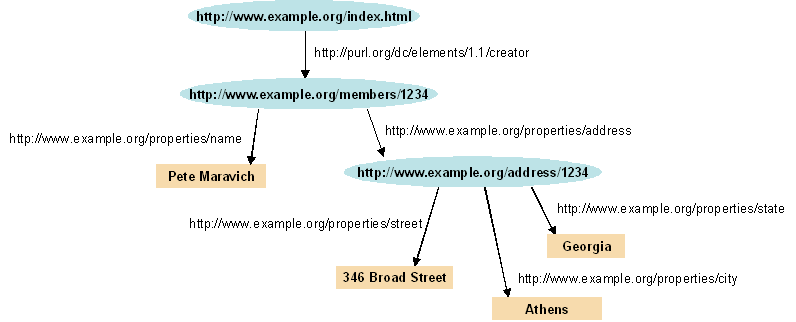
\includegraphics[width=\linewidth]{rdf.png}
	\caption{Example of RDF representation of an address}
	\label{fig:rdfGraph}
\end{figure}

Several methods exist for serializing the RDF data model. The most common format is RDF/XML. There exist other text-based formats introduced by W3C such as Turtle\footnote{\url{http://www.w3.org/TeamSubmission/turtle}} and N-Triples\footnote{\url{http://www.w3.org/TR/n-triples}} which are easier to read than RDF/XML.

RDF also contains data structures (containers and collections) that allow aggregating nodes or facts together. They are basically a syntactic sugar that will ease the process of writing code with no semantic expressiveness whatsoever.

\subsection{RDF Schema}

\begin{flushright}
	\textit{``It's impossible to get everyone everywhere to agree on a single label for every specific thing that ever was, is, or shall be''}\\
	Cambridge Semantics~\cite{Cambridge:RDF-101:13}
\end{flushright}

RDF is a simple and flexible data model that describes resources using properties and values. Predicates in RDF are what describe and give meaning to statements. They act as a vocabulary or an ontology. An Ontology is an explicit specification of a conceptualization~\cite{Gruber:KA:93}. It is a formal way to organize knowledge and terms and reflect common understanding of a domain. Ontologies are typically represented as graphical relationships or networks as opposed to taxonomies which are usually presented hierarchically. Some core elements of an ontology are:

\begin{itemize}
	\item Class: defines a concept, type or collection within a specific domain. It encapsulates objects sharing some properties. For instance, in a geographical domain, the class Country is more specialized than the class Place.
	\item Individual: also known as instance or object and is a member of a class. For instance, \emph{France} is an instance of the class Country.
	\item Property: is a binary relation describing how classes and individuals relate to each other. A datatype property connects instances with RDF literals while object property connects instances of two classes. For example, \emph{hasCity} is an object property that can relate two instances of the class City.
\end{itemize}

In order for Semantic Web applications to be able to share data, they must agree on common vocabulary. RDF doesn't provide ways to define those vocabularies and to specify domain specific classes and properties. To overcome this limitation, an extension of RDF called RDF Schema (RDFS)~\cite{Brickley:RDFS:14} provides a basic vocabulary to interpret RDF statements, describes taxonomies of classes and properties and defines very basic restrictions.

RDFS as a modeling language allows for: 1) definition of classes and their instantiation, 2) definition of properties and restrictions and 3) definition of hierarchies for classes and properties. In summary:

\begin{itemize}
	\item Resources are instances of one or more class (\emph{rdfs:class}). Classes are organized in a hierarchy using~\emph{rdfs:subClassOf} property.
	\item Properties have are assigned the class \emph{rdf:Property} and are organized in a hierarchy using~\emph{rdfs:subPropertyOf}.
	\item Restrictions on properties can be specified. For example,~\emph{rdfs:domain} to define the class of the subject and \emph{rdfs:range} to define the class of the object.
\end{itemize}

\subsection{Web Ontology Language}

RDFS provides basic hierarchies associated with simple restrictions. This limited expressivity triggered the need to define an explicit formal description of concepts in complex domains. As a result, the Web Ontology Language (OWL)~\cite{W3C:OWL:12} which adds more vocabulary for describing properties and classes on top of RDF is the current markup language endorsed by W3C. It provides more relations between classes (e.g. \emph{disjointWith}), logical properties (e.g. \emph{intersectionOf}, \emph{sameAs}) and enumerations (e.g. \emph{oneOf}, \emph{allValuesFrom}), among others.

\subsection{SPARQL Query Language}

Relational databases can be efficient for semantic databases. However, in practice, they are designed for a different type of workload. The fundamental operation of semantic databases is join, which is naturally expensive in relational databases. Given that we have our data modeled as RDF regardless of the underlying database choice, it is now possible to query and ask questions about our data in a very powerful way. Protocol and RDF Query Language (SPARQL)~\cite{Prud:SPARQL:08} is the standardized query language for RDF.

A SPARQL query consists of a set of triples where each part (subject, predicate and/or object) can consist of variables alongside a set of conjunctions (e.g. logical ``and'') or disjunctions (e.g. logical ``or''). It works by matching the triples in the query with the existing RDF triples and find solutions to the variables.

\subsection{Linked Data}

The traditional approach of sharing data through independent silos is diminishing with the various advances in the Web. The Semantic Web envisages the availability of large amount of interlinked RDF data. Linked Data (LD) is a major milestone towards achieving this vision. Formally, Linked Data has been defined as about ``data published on the Web in such a way that it is machine readable, its meaning is explicitly defined, it is linked to other external datasets, and can in turn be linked to from external datasets''~\cite{Bizer:IJSWIS:09}.

\begin{figure}[ht!]
	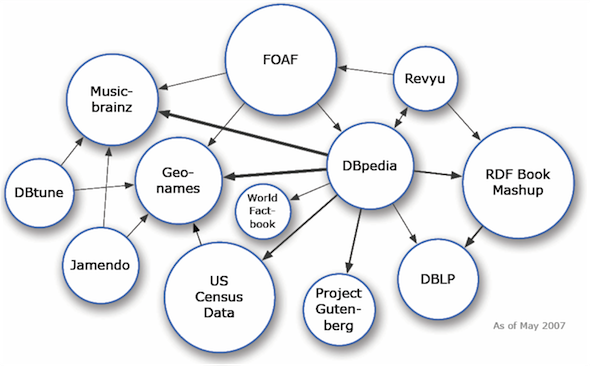
\includegraphics[width=0.9\textwidth]{lod-cloud2007.png}
	\caption{The LOD cloud as of May, 2007}
	\label{fig:lodcloud2007}
\end{figure}

Linked Data follows four main principles outlined by Tim Berners-Lee~\cite{Berners-Lee:W3C:06} to publish information on the Web, which are:

\begin{enumerate}
	\item Use URIs as names for things
	\item Use HTTP URIs so that people can look up those names.
	\item When someone looks up a URI, provide useful information, using the standards (RDF, SPARQL)
	\item Include links to other URIs. so that they can discover more things.
\end{enumerate}

Linked Data is continuously evolving, started in 2007 with a dozen of datasets (see Figure~\ref{fig:lodcloud2007}) to reach today thousands of datasets covering knowledge from various domains such as encyclopedic, government, geographic, entertainment, publications and so on. The datasets have tripled in size from 2011 to 2014, with a significant growth of nearly $271\%$~\cite{Schmachtenberg:ISWC:14}. The latest version published in April 2014 contains 1014 linked datasets connected by 2909 linksets (see Figure~\ref{fig:lodcloud2014}\footnote{A more Web friendly version can be accessed at~\url{http://data.dws.informatik.uni-mannheim.de/lodcloud/2014/}}).

One of the most widely used datasets is DBpedia\footnote{http://dbpedia.org}. It is a structured knowledge extracted from multilingual versions of Wikipedia~\cite{Bizer:WebSemJorunal:09}. At the time of writing, the English version of DBpedia consists of 470 millions RDF triples that describe 4.0 million things covering a wide range of topics, and contains 45 million RDF links to several hundred external datasets.

In order to achieve the Linked Data vision, datasets should contain outbound links to other datasets. Significant efforts try to automatically or semi-automatically generate these link to facilitate data discovery and to attach additional information.

\section{Open Data}\label{section:openData}

Open Data (OD) is the data that can be easily discovered, accessed, reused and redistributed by anyone~\cite{Davies:Report:15}. Open data should have both legal and technical dimensions. It should be placed in the public domain under liberal terms of use with minimal restrictions and should be available in electronic formats that are non-proprietary and machine readable. Similarly, Linked Open Data (LOD) refers to the semantically linked, machine-readable open data.

Businesses, citizens and governments are encouraged to publish, share and reuse data. Figure~\ref{fig:opendata_ecosystem} shows the Open Data ecosystem described by~\cite{Deloitte:Report:12}. Each party in this ecosystem supplies different types of data (e.g. Open Business Data (OBD), Open Government Data (OGD)) to different types of stakeholders.

\begin{figure}[ht!]
	\centering{
	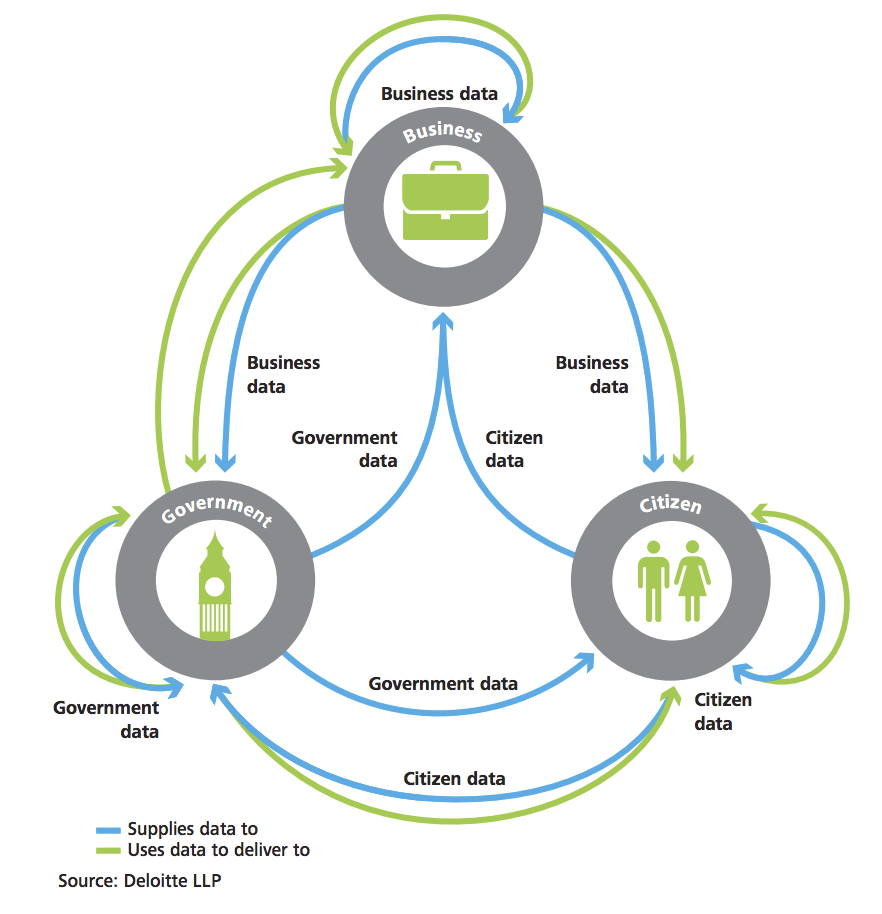
\includegraphics[width=0.7\textwidth]{opendata_ecosystem.png}
	\caption{Open Data ecosystem}
	\label{fig:opendata_ecosystem}
	}
\end{figure}

Similarly to the Linked Data principles, Tim Berners-Lee~\cite{Berners-Lee:W3C:06} outlined a 5 starts scheme to evaluate the availability of Linked Data as Linked Open Data:

\begin{enumerate}
	\item Data available on the web in any format, even using PDF or image scan, but with an Open license.
	\item Data delivered as machine-readable structured data, e.g. excel instead of image scan of a table.
	\item Data available in a non-proprietary format, e.g. CSV instead of excel.
	\item All the above plus, data using open standards from W3C, e.g. RDF and SPARQL, to identify things and properties, so that people can point at other data.
	\item All the above, plus, to link data to other people's data to provide context.
\end{enumerate}

Open Data has major benefits for citizens, businesses, societies and governments. It increases transparency and enables self-empowerment by improving the visibility of previously inaccessible information; allows citizens to be better informed about policies, public spending and activities in the law making processes~\cite{Deloitte:Report:12, Manyika:Report:13}.

Open Data is considered a gold mine for organizations which are trying to leverage external data sources in order to produce more informed business decisions~\cite{Boyd:Article:11}. Despite the legal issues surrounding Open Data licenses~\cite{Prateek:Misc:13}, McKinsey~\cite{Manyika:Report:13} estimates that Open Data in the health sector alone adds up over \$300 billion to the economy every year.

These huge benefits led to a world-wide adoption of Open Data. Figure~\ref{fig:god_adoption} shows the existence and support for open data initiatives, engagement with open data from outside government, legislative frameworks that support open data and the existence of training and support for data use and innovation~\cite{Davies:Report:15}.
Moreover, there are several reports and initiatives like Open Data Barometer\footnote{\url{http://barometer.opendataresearch.org/}}, Open Data Monitor\footnote{\url{http://opendatamonitor.eu}} and Global Open Data Index\footnote{\url{http://index.okfn.org/}}that aim at analyzing and monitoring the adoption of Open Data across the world.

Going back to our scenario in~\ref{section:scenario}, Open Data will help our analyst \textbf{Bob} in:

\begin{itemize}
	\item Have a transparent view on the data available by Ministry of Transport in France. This helps in preventing the possibility of wasting time and funds recollecting data that has been already collected by a different department.
	\item Discover complementary datasets from other sources. The benefits of data transparency amplifies when it is widely adopted in all other departments and agencies.The additional data enrich reports and enable better-informed, data-driven decisions. For example, by providing extra details on traffic information at the time when accidents occurred, \textbf{Bob} could draw more accurate conclusions on the root cause of some of these accidents.
\end{itemize}

\begin{figure}[ht!]
	\centering{
	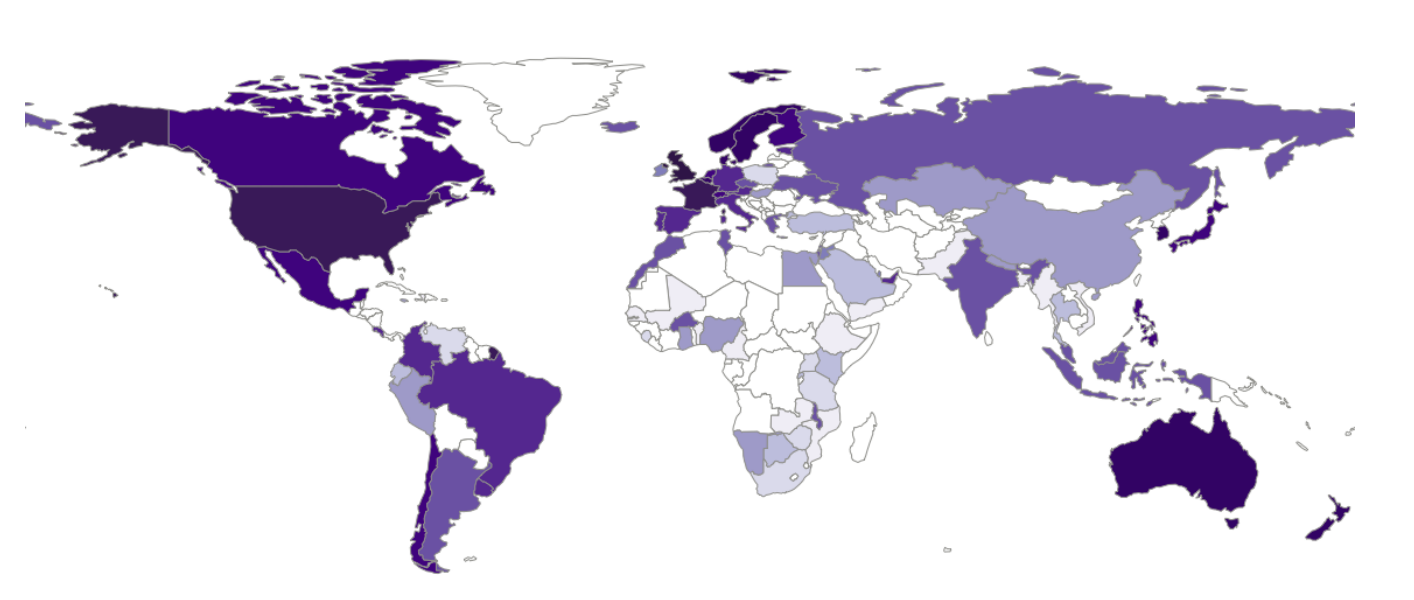
\includegraphics[width=0.9\textwidth]{god_adoption.png}
	\caption{Heat map of Open Government Data adoption according to the Open Data Barometer 2015}
	\label{fig:god_adoption}
	}
\end{figure}

\subsection{Open Licenses}

Project Open Data~\footnote{https://project-open-data.cio.gov} emphasizes the importance of datasets reusability as one of the main principles for Open Data. Open data should be made available under an open license. This is of high importance specially for organizations looking to integrate data for commercial use.

The Open Definition~\footnote{http://opendefinition.org/} defines a license as the legal conditions under which an item or piece of knowledge (also referred to as ``work'') is made available. Domain dedications like \emph{Creative Commons Zero} satisfy this definition although not technically a ``license''.

The Open Definition defines the following conditions for open licenses:

\begin{itemize}
	\item Allow free use of the work without any fee arrangement or compensation.
	\item Allow redistribution (on its own or as part of a collection) of the work.
	\item Allow distribution of modified work under the same license of the original.
	\item Allow any part of the work to be freely used, distributed or modified separately.
	\item Allow distribution of the work alongside other distinct works without placing restrictions on the additional ones.
	\item Doesn't discriminate against any person or group.
	\item Allow use, redistribution, modification, and compilation for any purpose.
	\item Allow rights propagation to all to whom the work id distributed.
\end{itemize}

\begin{figure}[ht!]
	\centering{
	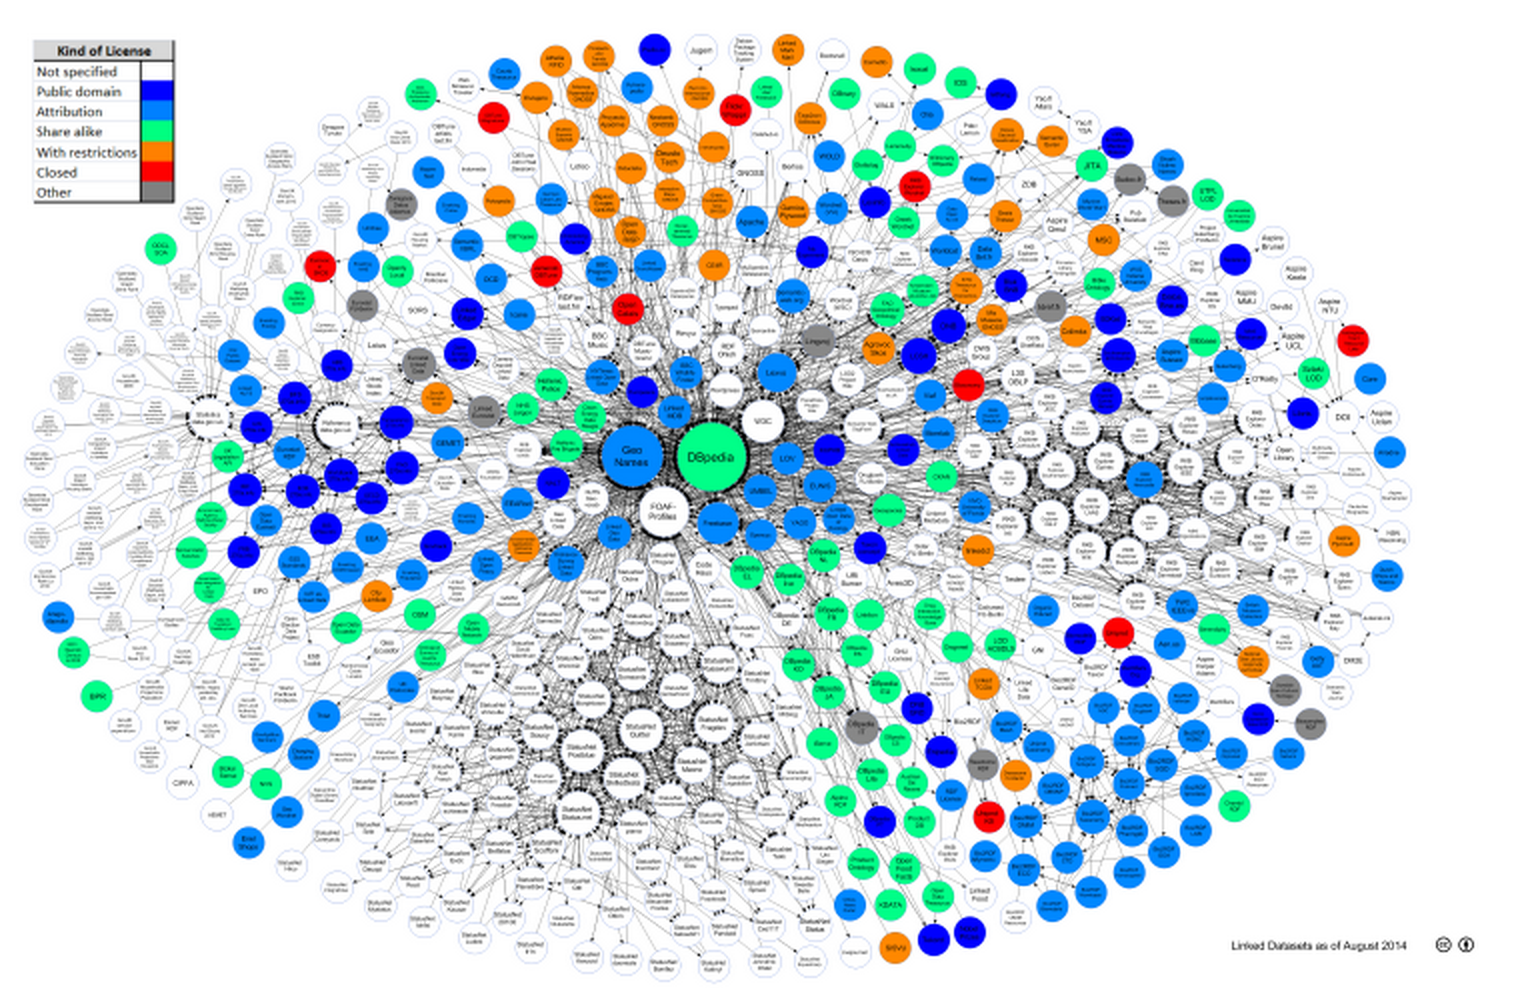
\includegraphics[width=0.9\textwidth]{lod14_licenses.png}
	\caption{Linking Open Data cloud diagram 2014, by Max Schmachtenberg, Christian Bizer, Anja Jentzsch and Richard Cyganiak colored by licensing types. \url{http://www.cosasbuenas.es/blog/how-o-is-lod-2015}}
	\label{fig:lodcloud2014}
	}
\end{figure}

\section{Data Profiling}\label{section:dataProfiling}

The huge amount of published data makes it difficult to discover relevant datasets through traditional inspection of the raw data. \textit{Data profiling} is the process of creating descriptive information and collect statistics about that data. It is a cardinal activity when facing an unfamiliar dataset~\cite{Li:WISM:12, Kimball:DWL:98}.

Data profiling is a vital task to monitor the quality of internal data in the enterprise. Halo BI report~\cite{Halo:TechReport:13} states that nearly 40\% of company's data is found to be inaccurate. 25\% of which is considered critical data.

Data profiles reflect the importance of datasets without the need for detailed inspection of the raw data.  It also helps in assessing the importance of the dataset, improving users' ability to search and reuse part of the dataset and in detecting irregularities to improve its quality. Data profiling includes typically several tasks:
\begin{itemize}
  \item \textbf{Metadata profiling}: Provides general information on the dataset (dataset description, release and update dates), legal information (license information, openness), practical information (access points, data dumps), etc.
  \item \textbf{Statistical profiling}: Provides statistical information about data types and patterns in the dataset (e.g. properties distribution, number of entities and RDF triples).
  \item \textbf{Topical profiling}: Provides descriptive knowledge on the dataset content and structure. This can be in form of tags and categories used to facilitate search and reuse.
  \item \textbf{Quality profiling}: Discovers inconsistencies and anomalies in the data. Data is considered of high quality if is appropriate for use and if it correctly represents the world constructs to which it refers~\cite{Juran:McGraw:99}.
\end{itemize}

Dataset profiles are collections of data describing the internal structure of the dataset. They are presented as a set of metadata in different formats such as JSON, XML and RDF. The Linked Data publishing best practices~\cite{Bizer:DB:11} specifies that datasets should contain metadata needed to effectively understand and use them. \textit{Metadata} is structured information that describes, explains, locates, or otherwise makes it easier to retrieve, use, or manage an information resource~\cite{NISO:TechReport:04}. Having rich metadata helps in enabling:
\begin{itemize}
  \item \textbf{Data discovery, exploration and reuse}: In~\cite{Graham:TechReport:11}, it was found that users are facing difficulties finding and reusing publicly available datasets. Metadata provides an overview of datasets making them more searchable and accessible. High quality metadata can be at times more important than the actual raw data especially when the costs of publishing and maintaining such data is high.
  \item \textbf{Organization and identification}: The increasing number of datasets being published makes it hard to track, organize and present them to users efficiently. Attached metadata helps in bringing similar resources together and distinguish useful links.
  \item \textbf{Archiving and preservation}: There is a growing concern that digital resources will not survive in usable forms to the future~\cite{NISO:TechReport:04}. Metadata can ensure resources survival and continuous accessibility by providing clear provenance information to track the lineage of digital resources and detail their physical characteristics.
\end{itemize}

\section{Data Portals}\label{section:dataPortals}

Data portals (or data catalogs) are the entry points to discover published datasets. They are a curated collections of datasets metadata that provide a set of complementary discovery and integrations services.

Data portals can be public like \texttt{Datahub.io} and \texttt{publicdata.eu} or private ones like \texttt{quandl.com} and \texttt{enigma.io}. Private portals harness manually curated data from various sources and expose them to users either freely or through paid plans. Similarly, in some public data portals, administrators manually review datasets information, validate, correct and attach suitable metadata information. This information is mainly in the form of predefined tags such as \textit{media, geography, life sciences} for organization and clustering purposes.

There are several Data Management Systems (DMS) that power public data portals. CKAN\footnote{\url{http://ckan.org}} is the world's leading open-source data portal platform powering web sites like DataHub, Europe's Public Data and the U.S Government's open data. Modeled on CKAN, DKAN\footnote{\url{http://nucivic.com/dkan/}} is a standalone Drupal distribution that is used in various public data portals as well. Socrata\footnote{\url{http://www.socrata.com}} helps public sector organizations improve data-driven decision making by providing a set of solutions including an open data portal. In addition to these tradition data portals, there is a set of tools that allow exposing data directly as RESTful APIs like \texttt{thedatatank.com}.
\clearpage

%% Part 1
\part{Structuring and Linking Event-centric Data on the Web} \label{pa:part1}
\chapter*{Overview of Part \ref{pa:part1}}

In Part~\ref{pa:part1}, we focus on the development of a framework that retrieves and links event-centric information derived from event directories, media platforms and social networks. We capitalize on Semantic Web technologies to ensure a flexible and large-scale integration of disparate data sources, some of which overlap in their coverage. The goal is to provide a support for exploring and selecting events associated with media, and for discovering meaningful connections between them. 
\\
\\
In Chapter~\ref{ch:data-aggregation}, we present the different steps in building a large dataset called EventMedia which is composed of event descriptions associated with media. These steps include data aggregation and structuring into a unified knowledge model using ontologies. One fundamental requirement is to set a flexible architecture, so that it can easily support the addition of event and media Web services.
\\
\\
In Chapter~\ref{ch:data-reconciliation}, we focus on the fourth element of the Linked Data principles which is to link data together. The goal is to explore the implicit overlap of the disparate data sources trying to overcome some well-known types of data heterogeneity. We mainly investigate the following questions: what heuristics are suitable to reconcile event-centric information in Linked Data? How to align structured events with unstructured media content? 
\chapter{Consuming Linked Data in Event Domain}  \label{ch:web-app}
\graphicspath{{Part2/Chapter1/figures/}}

\section{Introduction}
\label{sec:introduction}
From 12 datasets cataloged in 2007, the Linked Open Data cloud has grown to nearly 1000 datasets containing more than 82 billion triples\footnote{http://datahub.io/dataset?tags=lod}~\cite{BizerHeath2009}. Data is being published by both the public and private sectors and covers a diverse set of domains from life sciences to media or government data. The Linked Open Data cloud is potentially a gold mine for organizations and individuals who are trying to leverage external data sources in order to produce more informed business decisions~\cite{Boyd2011}. This success lies in the cooperation between data publishers and consumers. Consumers are empowered to find, share and combine information in their applications easily. However, the heterogeneous nature of data sources reflects directly on the data quality as these sources often contain inconsistent as well as misinterpreted and incomplete metadata information. Considering the significant variation in size, the languages used and the freshness of the data, one realizes that finding useful datasets without prior knowledge is increasingly complicated. This can be clearly noticed in the LOD Cloud where few datasets such as DBPedia~\cite{Bizer:2009:DCP:1640541.1640848}, Freebase~\cite{Bollacker:2008:FCC:1376616.1376746} and YAGO~\cite{Suchanek:2007:YCS:1242572.1242667} are favored over less popular datasets that may include domain specific knowledge more suitable for the tasks at hand. For example, for the task of building context-aware recommender systems in an academic digital library over LOD cloud, popular datasets like Semantic Web Dog Food, DBLP or Yovisto can be favored over lesser known but more specific datasets like VIAF\footnote{http://datahub.io/dataset/viaf} which links authority files of 20 national libraries, list of subject headings for public libraries in Spain\footnote{http://datahub.io/dataset/lista-encabezamientos-materia} or the French dissertation search engine\footnote{http://datahub.io/dataset/thesesfr}.

The main entry point for discovering and identifying datasets is either through public data portals such as DataHub\footnote{http://datahub.io} and Europe's Public Data\footnote{http://publicdata.eu} or private search engines such as Quandl\footnote{https://quandl.com/} and Engima\footnote{http://enigma.io/}. Private portals harness manually curated data from various sources and expose them to users either freely or through paid plans. The data available is of higher quality but lesser quantity compared to what is available in public portals. Similarly, in some public data portals, administrators manually review datasets information, validate, correct and attach suitable metadata information. This information is mainly in the form of predefined tags such as \textit{media, geography, life sciences} for organization and clustering purposes. However, the diversity of those datasets makes it harder to classify them in a fixed number of predefined tags that can be subjectively assigned without capturing the essence and breadth of the dataset~\cite{6690016}. Furthermore, the increasing number of datasets available makes the metadata review and curation process unsustainable even when outsourced to communities.

\textit{Data profiling} is the process of creating descriptive information and collect statistics about that data. It is a cardinal activity when facing an unfamiliar dataset~\cite{semwebprofiling}. It helps in assessing the importance of the dataset, in improving users' ability to search and reuse part of the dataset and in detecting irregularities to improve its quality. Data profiling includes typically several tasks:
\begin{itemize}
  \item \textbf{Metadata profiling}: Provides general information on the dataset (dataset description, release and update dates), legal information (license information, openness), practical information (access points, data dumps), etc.
  \item \textbf{Statistical profiling}: Provides statistical information about data types and patterns in the dataset, i.e. properties distribution, number of entities and RDF triples, etc.
  \item \textbf{Topical profiling}: Provides descriptive knowledge on the dataset content and structure. This can be in form of tags and categories used to facilitate search and reuse.
\end{itemize}

In this work, we address the challenges of automatic validation and generation of descriptive datasets profiles. This paper proposes an extensible framework consisting of a processing pipeline that combines techniques for data portals identification, datasets crawling and a set of pluggable modules combining several profiling tasks. The framework validates the provided dataset metadata against an aggregated standard set of information. Metadata fields are automatically corrected when possible, e.g. adding a missing license URL reference. Moreover, a report describing all the issues highlighting those that cannot be automatically fixed is created to be sent by email to the dataset's maintainer. There exist various statistical and topical profiling tools for both relational and Linked Data. The architecture of the framework allows to easily add them as additional profiling tasks. However, in this paper, we focus on the task of dataset metadata profiling and present our findings by running our framework on the LOD cloud. The results demonstrate that the general state of LOD cloud needs more attention as most of the datasets suffer from bad quality metadata lacking some informative metrics needed to facilitate dataset search. The noisiest metadata are the access information such as licensing information, resource descriptions as well as resource availability problems.

The remainder of the paper is structured as follows. In Section~\ref{sec:related-work}, we review relevant related work. In Section~\ref{sec:framework}, we describe our proposed framework's architecture and components that validate and generate dataset profiles. In Section~\ref{sec:experiment}, we present the results when running this tool on the LOD cloud and we summarize the main issues found. Finally, we conclude and outline some future work in Section~\ref{sec:conclusion}.

%%%%%%%%%%%%%%%%%%%%%%%%%
%%%  2. Related Work  %%%
%%%%%%%%%%%%%%%%%%%%%%%%%

\section{Related Work}
\label{sec:related-work}
There exists a considerable amount of tools that tackle specific profiling tasks. For example, \cite{6816740}\cite{makela-aether-2014} focus on generating statistical dataset information where in \cite{6690016}\cite{scalableApproach} authors use various techniques to attach additional topical information. However, to the best of our knowledge, this is the first effort towards extensible automatic validation and generation of descriptive dataset profiles. For this paper, we will focus on Linked Data metadata profiling tasks. However, one of the advantages of this framework is the ability to easily configure additional profiling tasks e.g. statistical or topical and accommodate different data types e.g. relational.\\

Data Catalog Vocabulary (DCAT) \cite{Erickson:14:DCV} and the Vocabulary of Interlinked Datasets (VoID) \cite{Cyganiak:11:DLD} are concerned with metadata about RDF datasets. There exist several tools aiming at exposing dataset metadata using these vocabularies. In \cite{BoHm:2011:CVD:2030805.2031001} authors generate VoID descriptions limited to a subset of properties that can be automatically deduced from resources within the dataset. However, it still provides data consumers with interesting insights. Quality Assessment of Data Sources (Flemming's Data Quality Assessment Tool)\footnote{http://linkeddata.informatik.hu-berlin.de/LDSrcAss/datenquelle.php} provides basic metadata assessment as it calculates data quality scores based on manual user input. The user assigns weights to the predefined quality metrics and answer a series of questions regarding the dataset. These include, for example, the use of obsolete classes and properties by defining the number of described entities that are assigned disjoint classes, the usage of stable URIs and whether the publisher provides a mailing list for the dataset. The ODI certificate\footnote {https://certificates.theodi.org/} on the other hand provides a description of the published data quality in plain English. It aspires to act as a mark of approval that helps publishers understand how to publish good open data and users how to use it. It gives publishers the ability to provide assurance and support on their data while encouraging further improvements through an ascending scale. ODI comes as an online and free questionnaire for data publishers focusing on certain characteristics about their data. Although these approaches try to perform metadata profiling, they are either incomplete or manual. In our framework, we propose a more automatized and complete approach.\\
The Project Open Data Dashboard\footnote{http://labs.data.gov/dashboard/} tracks and measures how US government websites implement the Open Data principles to understand the progress and current status of their public data listings. A validator analyzes machine readable files e.g. JSON files for automated metrics like the resolved URLs, HTTP status and content-type. However, deep schema information about the metadata is missing like description, license information or tags. Similarly on the LOD cloud, the Data Hub LOD Validator\footnote{http://validator.lod-cloud.net/} gives an overview of Linked Data sources cataloged on the Data Hub. It offers a step-by-step validator guidance to check a dataset completeness level for inclusion in the LOD cloud. The results are divided into four different compliance levels from basic to reviewed and included in the LOD cloud. Although it is an excellent tool to monitor LOD compliance, it still lacks the ability to give detailed insights about the completeness of the metadata and overview on the state of the whole LOD cloud group and is very specific to the LOD cloud group rules and regulations.\\
Although the above mentioned tools are able to provide various information about a dataset, there exist no approach that is extensible to combine further information coming from various profiling tools.

\textbf{Statistical profiling}: Calculating statistical information on datasets is vital to applications dealing with query optimization and answering, data cleansing, schema induction and data mining \cite{profilingWebOfData} \cite{datafinland2} \cite{6690016}. Semantic sitemaps \cite{Cyganiak:2008:SSE:1789394.1789457} and RDFStats \cite{Langegger:2009:RER:1674635.1674691} where one of the first to deal with RDF data statistics and summaries. ExpLOD \cite{Khatchadourian:2010:ESE:2155278.2155300} creates statistics on the interlinking between datasets based on \texttt{owl:sameAs} links. In \cite{semwebprofiling} the author introduces a tool that induces the actual schema of the data and gather corresponding statistics accordingly. LODStats  \cite{Auer:2012:LEF:2413941.2413982} is a stream-based approach that calculates more general dataset statistics. ProLOD++ \cite{6816740} is a Web-based tool that allows LOD analysis via automatically computed hierarchical clustering \cite{5452762}. Aether \cite{makela-aether-2014} generates VoID statistical descriptions of RDF datasets. It also provides a Web interface to view and compare VoID descriptions. LODOP \cite{forchhammer_profiles_2014} is a MapReduce framework to compute, optimize and benchmark dataset profiles. The main target for this framework is to optimize the runtime costs for Linked Data profiling. In \cite{DyLDO} authors calculate certain statistical information for the purpose of observing the dynamic changes in datasets.\\

\textbf{Topical Profiling}: Topical and categorical information facilitates dataset search and reuse. Topical profiling focuses on content-wise analysis at the instances and ontological levels. GERBIL \cite{gerbil} is a general entity annotation framework that provides machine processable output allowing efficient querying. In addition, there exist several entity annotation tools and frameworks \cite{Cornolti:2013:FBE:2488388.2488411} but none of those systems are designed specifically for dataset annotation. In \cite{datafinalnd}, authors created a semantic portal to manually annotate and publish metadata about both LOD and non-RDF datasets. In \cite{6690016}, authors automatically assigned Freebase domains to extracted instance labels of some of the LOD Cloud datasets. The goal was to provide automatic domain identification, thus enabling improving datasets clustering and categorization. In \cite{Bohm:2012:LTG:2396761.2398718}, authors extracted dataset topics by exploiting the graph structure and ontological information, thus removing the dependency on textual labels. In  \cite{scalableApproach} authors generate VoID and VoL descriptions via a processing pipeline that extracts dataset topic models ranked on graphical models of selected DBpedia categories.\\

Dataset search can be done without relying on attached metadata (tags and categories). For example, there exist several approaches to create LOD indexes. In \cite{Alexander:LDOW09}, authors used VoID descriptions to optimize query processing by determining relevant query-able datasets. In \cite{Harth:2010:DSO:1772690.1772733}, authors created an approximate index structure (QTree) and an algorithm for answering conjunctive queries over Linked Data. SchemEX \cite{Konrath:2012:SEC:2399444.2399563} is a stream-based approach leveraging type and property information of RDF instances to create schema-level indexes.\\
Semantic search engines like Sindice \cite{Delbru2010a}, Swoogle \cite{Ding2004} and Watson \cite{d'Aquin:2011:WMS:2019470.2019476} help in entities lookup but are not designed specifically for dataset search. In \cite{whatShouldILinkTo}, authors utilized the sig.ma index \cite{sig.ma} to identify appropriate data sources for interlinking. However, the current main source for dataset search and discovery is via data portals. CKAN and DKAN powered data portals rely on attached metadata to provide dataset search features as they run a Solr index on the metadata schemas. Having missing or inconsistent information will affect the search results quality.

%%%%%%%%%%%%%%%%%%%%%%%%%%%%%%%%%%%
%%%  3. Profiling data portals  %%%
%%%%%%%%%%%%%%%%%%%%%%%%%%%%%%%%%%%

\section{Profiling Data Portals}
\label{sec:framework}

In this section, we provide an overview of the processing steps for validating and generating dataset profiles. Figure \ref{fig:1} shows the main steps which are the following: (i) Data portal identification; (ii) metadata extraction; (iii) instance and resource extraction; (iv) profile validation (v) profile and report generation.

Our framework is built as a Command Line Interface (CLI) application using Node.js. Instructions on installing and running the framework are available on its public Github repository\footnote{https://github.com/ahmadassaf/opendata-checker}. Related functions are encapsulated into modules that can be easily plugged in/out the processing pipeline. The various steps are explained in details below.

\begin{figure}[!ht]
  \centering
    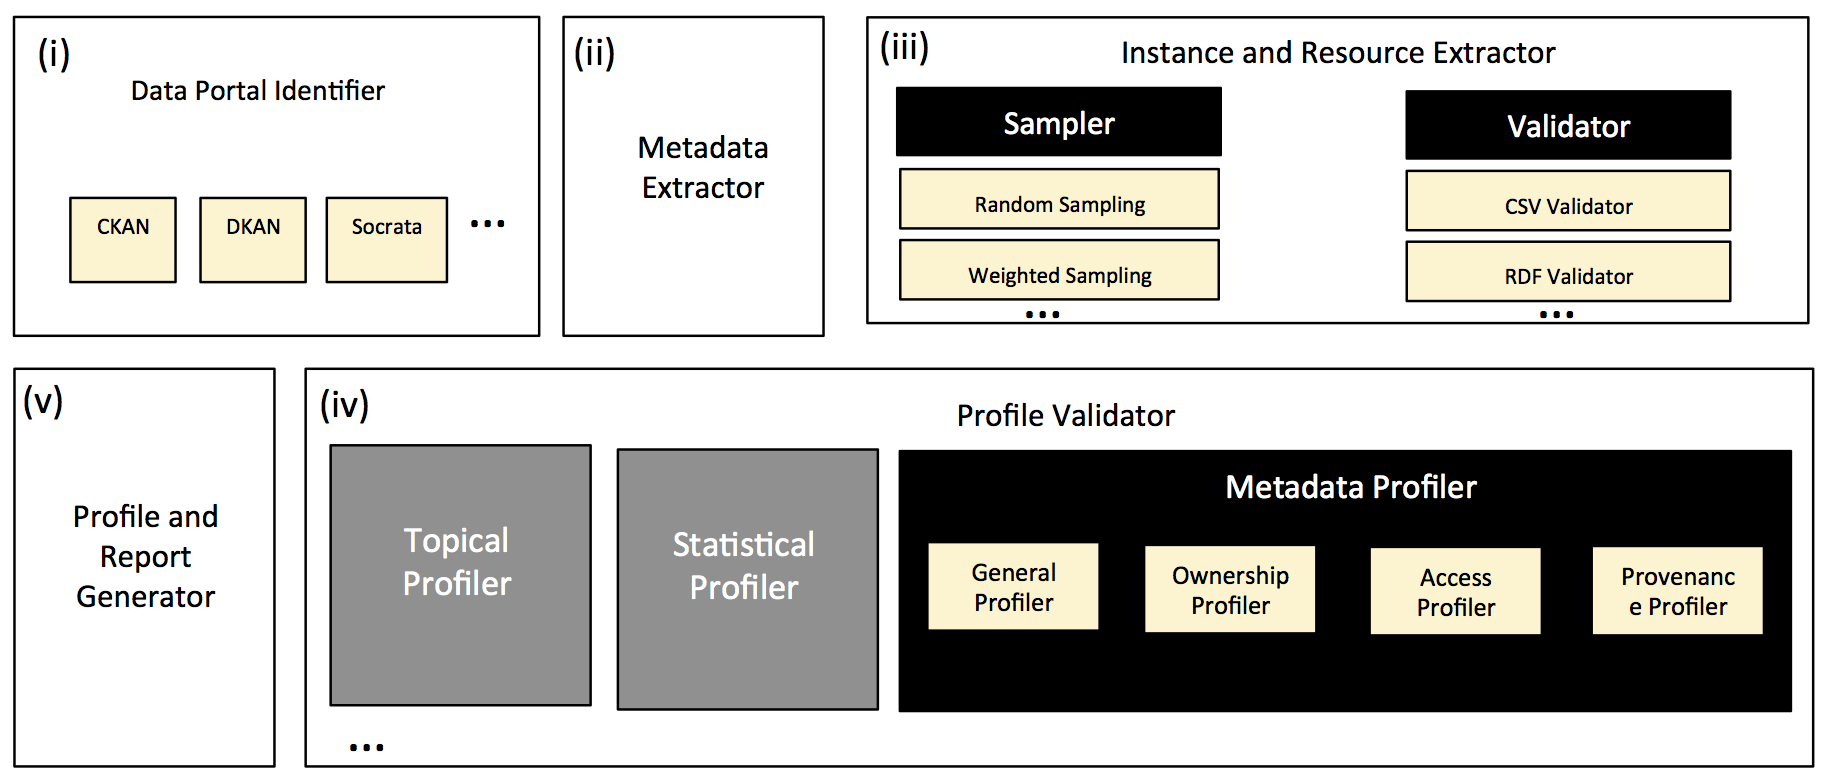
\includegraphics[scale=0.4]{figure-1_architecture.png}
  \caption{Processing pipeline for validating and generating dataset profiles}
  \label{fig:1}
\end{figure}

\subsection{Data Portal Identification}

Data portals can be considered as data access points providing tools to facilitate data publishing, sharing, searching and visualization. CKAN\footnote{http://ckan.org} is the world's leading open-source data portal platform powering websites like the DataHub, Europe's Public Data and the U.S Government's open data. Modeled on CKAN, DKAN\footnote{http://drupal.org/project/dkan} is a standalone Drupal distribution that is used in various public data portals as well. Socrata\footnote{http://www.socrata.com} helps public sector organizations improve data-driven decision making by providing a set of solutions including an open data portal. In addition to these tradition data portals, there is a set of tools that allow exposing data directly as RESTful APIs like Datatank\footnote{http://thedatatank.com} and Database-to-API\footnote{https://github.com/project-open-data/db-to-api}.

Identifying the software powering data portals is a vital first step to understand the API calls structure. Web scraping is a technique for extracting data from Web pages. We rely on several scraping techniques in the identification process which includes a combination of the following:

\begin{itemize}
  \item \textbf{URL inspection}: Check the existence of certain URL patterns. Various CKAN based portals are hosted on subdomains of the \texttt{http://ckan.net}. For example, CKAN Brazil (\texttt{http://br.ckan.net}).
  \item \textbf{Meta tags inspection}: The \texttt{<meta>} tag provides metadata about the HTML document. They are used to specify page description, keywords, author, etc. Inspecting the \texttt{content} attribute can indicate the type of the data portal. We use CSS selectors to check the existence of these meta tags. An example of a query selector is \texttt{meta[content*="ckan]} (all meta tags with the attribute content containing the string $CKAN$). This selector can identify CKAN portals whereas the \texttt{meta[content*="Drupal"]} can identify DKAN portals.
  \item \textbf{Document Object Model (DOM) inspection}: Similar to the meta tags inspection, we check the existence of certain DOM elements or properties. For example, CKAN powered portals will have DOM elements with class names like \texttt{ckan-icon} or \texttt{ckan-footer-logo}. A CSS selector like \texttt{.ckan-icon} will be able to check if a DOM element with the class name \texttt{ckan-icon} exists.\\
  The list of elements and properties to inspect is stored in a separate configurable object for each portal. This allows the addition and removal of elements as deemed necessary.
\end{itemize}

The identification process for each portal can be easily customized by overriding the default function. Moreover, adding or removing steps from the identification process can be easily configured.\\
After those preliminary checks, we query one of the portal's API endpoints. For example, DataHub is identified as CKAN, so we will query the API endpoint on \texttt{http://datahub.io/api/action/package\_list}. A successful request will list the names of the site's datasets, whereas a failing request will signal a possible failure of the identification process.

\subsection{Metadata Extraction}

Data portals expose a set of information about each dataset as metadata. The model used varies across portals. However, a standard model should contain information about the dataset's title, description, maintainer email, update and creation date, etc. We divided the metadata information into the following:

\textbf{General information}: General information about the dataset. e.g. title, description, ID, etc. This general information is manually filled by the dataset owner. In addition to that, tags and group information is required for classification and enhancing dataset discoverability. This information can be entered manually or inferred modules plugged into the topical profiler.

\textbf{Access information}: Information about accessing and using the dataset. This includes the dataset URL, license information i.e. license title and URL and information about the dataset's resources. Each resource has as well a set of attached metadata e.g. resource name, URL, format, size, etc.

\textbf{Ownership information}: Information about the ownership of the dataset. e.g. organization details, maintainer details, author, etc. The existence of this information is important to identify the authority on which the generated report and the newly corrected profile will be sent to.

\textbf{Provenance information}: Temporal and historical information on the dataset and its resources. For example, creation and update dates, version information, version, etc. Most of this information can be automatically filled and tracked.

Building a standard metadata model is not the scope of this paper, and since we focus on CKAN-based portals, we validate the extracted metadata against the CKAN standard model\footnote{http://demo.ckan.org/api/3/action/package\_show?id=adur\_district\_spending}.\\
After identifying the underlying portal software, we perform iterative queries to the API in order to fetch datasets metadata and persist them in a file-based cache system.
Depending on the portal software we can issue specific extraction jobs. For example, in CKAN based portals, we are able to crawl and extract the metadata of a specific dataset, all the datasets in a specific group e.g. LOD Cloud or all the datasets in the portal.

\subsection{Instance and Resource Extraction}

From the extracted metadata we are able to identify all the resources associated with that dataset. They can have various types like a SPARQL endpoint, API, file, visualization ,etc. However, before extracting the resource instance(s) we perform the following steps:

\begin{itemize}
  \item \textbf{Resource metadata validation and enrichment}: Check the resource attached metadata values. Similar to the dataset metadata, each resource should include information about its mimetype, name, description, format, valid de-referenceable URL, size, type and provenance. The validation process issue an HTTP request to the resource and automatically fills up various missing information when possible, like the mimetype and size by extracting them from the HTTP response header. However, missing fields like name and description that needs manual input are marked as missing and will appear in the generated summary report.
  \item \textbf{Format validation}: Validate specific resource formats against a linter or a validator. For example, node-csv\footnote{https://github.com/wdavidw/node-csv} for CSV files and n3\footnote{https://github.com/RubenVerborgh/N3.js} to validate N3 and Turtle RDF serializations.
\end{itemize}

Considering that certain dataset contains large amounts of resources and the limited computation power of some machines on which the framework might run on, a sampler module is introduced to execute various sample-based strategies detailed in \cite{scalableApproach} where they were found to generate accurate results even with comparably small sample size of 10\%.

\begin{itemize}
  \item \textbf{Random Sampling}: Randomly selects resources instances.
  \item \textbf{Weighted Sampling}: Weighs each resources as the ratio of the number of datatype properties used to define a resource over the maximum number of datatype properties over all the datasets resources.
  \item \textbf{Resource Centrality Sampling}: Weighs each resource as the ration of the number of resource types used to describe a particular resource divided by the total number of resource types in the dataset. This is specific and important to RDF datasets where important concepts tend to be more structured and linked to other concepts.
\end{itemize}

However, the sampler is not restricted only to these strategies. Strategies like those introduced in \cite{Leskovec:2006:SLG:1150402.1150479} can be configured and applied in the processing pipeline.

\subsection{Profile Validation}

A dataset profile should include descriptive information about the data examined. In our framework, we have identified three main profiling information. However, the extensibility of our framework allows for additional profiling techniques to be plugged in easily i.e. a quality profiling module reflecting the dataset quality. In this paper, we focus on the task of metadata profiling.\\

Metadata validation process identifies missing information and the ability to automatically correct them. Each set of metadata (general, access, ownership and provenance) is validated and corrected automatically when possible. Each profiler task has a set of metadata fields to check against. The validation process check if each field is defined and if the value assigned is valid.

There exist a bunch of special validation steps for various fields. For example, for ownership information where the maintainer email has to be defined, the validator checks if the email field is an actual valid email address. A similar process is done to URLs whenever found. However, we also issue an HTTP \texttt{HEAD} request in order to check if that URL is reachable or not. For the dataset resources, we use the \texttt{content-header} information when the request is successfull in order to extract, compare and correct further metadata values like mimetype and content size.

Despite the legal issues surrounding Linked Data licenses \cite{nomoneyLOD}, it is still considered a gold mine for organizations who are trying to leverage external data sources in order to produce more informed business decisions \cite{Boyd2011}. In \cite{mckinseyreport} the authors see the potential economic effect unfolding in education, transportation, consumer products, electricity, oil and gas, health care and consumer finance. They estimate the potential annual value enabled by Open Data in these domains to be 3 trillion US Dollars across seven domains. As a result, validating license related information is vital. However, from our experiments, we found out that datasets' license information is noisy. The license names if found are not standardized. For example, Creative Commons CCZero can be also CC0 or CCZero. Moreover,the license URI if found and if de-referenceable can point to different reference knowledge bases e.g. \texttt{http://opendefinition.org}. To overcome this issue, we have manually created a mapping file standardizing the set of possible license names and the reference knowledge base\footnote{https://github.com/ahmadassaf/opendata-checker/blob/master/util/licenseMappings.json}. In addition, we have also used the open source and knowledge license information\footnote{https://github.com/okfn/licenses} to normalize the license information and add extra metadata like the domain, maintainer and open data conformance.

\lstset{frame=single, caption={License mapping file sample}, label=json, captionpos=b}
\begin{lstlisting}[language=json]
{
  "license_id" : ["ODC-PDDL-1.0"],
  "disambiguations" : ["Open Data Commons Public Domain Dedication and License (PDDL)"]
},
{
  "license_id" : ["CC-BY-SA-4.0", "CC-BY-SA-3.0"],
  "disambiguations" : ["cc-by-sa", "CC BY-SA","Creative Commons Attribution Share-Alike"]
}
\end{lstlisting}


\textbf{Statistical profiling}\\

There exist a set of tools designed specifically to provide statistical information about a dataset (see section 2). Providing comprehensive statistical information about a dataset isn't in the scope of this paper. However, to show the extensibility of our framework we provide a simple RDF statistical profiler module that can be easily extended and configured. The information provided for each class is the number: triples, distinct objects, distinct literals, distinct IRI reference objects, distinct blank nodes objects, distinct subjects, distinct IRI reference subjects and distinct blank nodes subjects.\\

\textbf{Topical profiling}\\

Similar to the statistical profiler, a detailed survey of the existing tools can be found in the related work section. However, we implement a very basic topical profiler by applying Named Entity Disambiguation (NED) on the textual description and title of a dataset using DBpedia Spotlight \cite{Mendes:2011:DSS:2063518.2063519}.

\subsection{Profile and Report Generation}

The validation process highlights the missing information and presents them in a human readable report. The report can be automatically sent to the dataset maintainer email if exists in the metadata.

In addition to the generated report, the enhanced profiles are represented in JSON using the CKAN data model and are publicly available\footnote{https://github.com/ahmadassaf/opendata-checker/tree/master/results}.

Data portal administrators need an overall knowledge of the portal datasets and their properties. Our framework has the ability to generate numerous reports of all the datasets by passing formated queries. There are two main set of aggregation tasks that can be run:
\begin{itemize}
  \item \textbf{Aggregating meta-field values}: Passing a string that corresponds to a valid field in the metadata. The field can be flat like \texttt{license\_title} (aggregates all the license titles used in the portal or in a specific group) or nested like \texttt{resource>resource\_type} (aggregates all the resources types for all the datasets). Such reports are important to have an overview of the possible values used for each metadata field.
  \item \textbf{Aggregating key:object meta-field values}: Passing two meta-field values separated by a colon \texttt{:} e.g. \texttt{resources>resource\_type:resources>name}. These reports are important as you can aggregate the information needed when also having the set of values associated to it printed.
\end{itemize}

For example, the meta-field value query \texttt{resource>resource\_type} run against the LODCloud group will result in an array containing $[file,api,documentation ...]$ values. These are all the resource types used to describe all the datasets of the group. However, to be able to know also what are the datasets containing resources corresponding to each type, we issue a key:object meta-field query \texttt{resource>resource\_type:name}. The result will be a JSON object having the \texttt{resource\_type} as the key and an array of corresponding datasets titles that has a resource of that type.

\lstset{basicstyle=\scriptsize, backgroundcolor=\color{white}, breaklines=true, frame=single, caption={Excerpt of the DBpedia validation report}, label=report, captionpos=b}
\begin{lstlisting}
=======================================================================
                      Metadata Report
=======================================================================
group information is missing. Check organization information as they can be mixed sometimes
organization_image_url field exists but there is no value defined
=======================================================================
                      Tag Statistics
=======================================================================
There is a total of: 21 [undefined] vocabulary_id fields  100.00%
=======================================================================
                      License Report
=======================================================================
License information has been normalized !
=======================================================================
                      Resource Statistics
=======================================================================
There is a total of: 10 [missing] url-type fields  100.00%
There is a total of: 9 [missing] created fields  90.00%
There is a total of: 10 [undefined] cache_last_updated fields  100.00%
There is a total of: 10 [undefined] webstore_last_updated fields  100.00%
There is a total of: 10 [undefined] size fields  100.00%
There is a total of: 10 [undefined] hash fields  100.00%
There is a total of: 10 [undefined] mimetype_inner fields  100.00%
There is a total of: 7 [undefined] mimetype fields  70.00%
There is a total of: 10 [undefined] cache_url fields  100.00%
There is a total of: 6 [undefined] name fields  60.00%
There is a total of: 9 [undefined] webstore_url fields  90.00%
There is a total of: 9 [undefined] last_modified fields  90.00%
There is one [undefined] format field  10.00%
=======================================================================
                      Resource Connectivity Issues
=======================================================================
There are 2 connectivity issues with the following URLs:
   - http://dbpedia.org/void/Dataset
=======================================================================
                      Un-Reachable URLs Types
=======================================================================
There are: 1 unreachable URLs of type [file]
\end{lstlisting}

%%%%%%%%%%%%%%%%%%%%%%%%%%%%%%%%%%%%%%%
%%%  4. Experiments and Evaluation  %%%
%%%%%%%%%%%%%%%%%%%%%%%%%%%%%%%%%%%%%%%

\section{Experiments and Evaluation}
\label{sec:experiment}

In this section, we provide the experiments and evaluation of the proposed framework. All the experiments are reproducible by our tool and their results are available on the its Github repository.\\
We have run the framework on the LOD cloud containing 259 datasets at the time of writing this paper. We ran the instance and resource extractor in order to cache the metadata files for these datasets locally and ran the validation process which took around one and a half hour on a 2.6 Ghz Intel Core i7 processor with 16GB of DDR3 memory machine.\\
A CKAN dataset metadata describes three main sections in addition to the core dataset's properties. Those are the groups, tags and resources. Each section contains a set of metadata corresponding to one or more metadata type. For example, a dataset resource will have general information such as the resource name, access information such as the resource url and provenance information such as creation date. The framework generates a report aggregating all the problems in all these sections, fixing field values when possible. Errors can be the result of missing metadata fields, undefined field values or field value errors e.g. unreachable URL or incorrect email address.

Figures \ref{fig:2} and \ref{fig:3} show the percentage of errors found in metadata fields by section and by information type respectively. We found out that the most erroneous information for the dataset core information were ownership related as 41\% were missing or undefined. Datasets resources have the poorest metadata. 64\% of the general metadata, all the access information and 80\% of the provenance information contained missing or undefined values. Table \ref{tab:main} shows the top metadata fields errors in each metadata information type.

\begin{center}
\begin{tabular}{|c|c|c|c|c|c|}

\hline
\multicolumn{2}{|c|}{Metadata Field} & Error \% & Section & Error Type & Auto Fix\tabularnewline
\hline
\hline
\multirow{6}{*}{General } & group & 100\% & Dataset & Missing & -\tabularnewline
\cline{2-6}
 & vocabulary\_id & 100\% & Tag & Undefined & -\tabularnewline
\cline{2-6}
 & url-type & 96.82\% & Resource & Missing & -\tabularnewline
\cline{2-6}
 & mimetype\_inner & 95.88\% & Resource & Undefined & Yes\tabularnewline
\cline{2-6}
 & hash & 95.51\% & Resource & Undefined & Yes\tabularnewline
\cline{2-6}
 & size & 81.55\% & Resource & Undefined & Yes\tabularnewline
\hline
\multirow{5}{*}{Access } & cahce\_url & 96.9\% & Resource & Undefined & -\tabularnewline
\cline{2-6}
 & webstore\_url & 91.29\% & Resource & Undefined & -\tabularnewline
\cline{2-6}
 & license\_url & 54.44\% & Dataset & Missing & Yes\tabularnewline
\cline{2-6}
 & url & 30.89\% & Resource & Unreachable & -\tabularnewline
\cline{2-6}
 & license\_title & 16.6\% & Dataset & Undefined & Yes\tabularnewline
\hline
\multirow{5}{*}{Provenance } & cache\_last\_updated & 96.91\% & Resource & Undefined & Yes\tabularnewline
\cline{2-6}
 & webstore\_last\_updated & 95.88\% & Resource & Undefined & Yes\tabularnewline
\cline{2-6}
 & created & 86.8\% & Resource & Missing & Yes\tabularnewline
\cline{2-6}
 & last\_modified & 79.87\% & Resource & Undefined & Yes\tabularnewline
\cline{2-6}
 & version & 60.23\% & Dataset & Undefined & -\tabularnewline
\hline
\multirow{5}{*}{Ownership } & maintainer\_email & 55.21\% & Dataset & Undefined & -\tabularnewline
\cline{2-6}
 & maintainer & 51.35\% & Dataset & Undefined & -\tabularnewline
\cline{2-6}
 & author\_email & 15.06\% & Dataset & Undefined & -\tabularnewline
\cline{2-6}
 & organization\_image\_url & 10.81\% & Dataset & Undefined & -\tabularnewline
\cline{2-6}
 & author & 2.32\% & Dataset & Undefined & -\tabularnewline
\hline
\end{tabular}
\captionof{table}{Top metadata fields error \% by type} \label{tab:main}
\end{center}

\begin{figure}

\parbox{7cm}{\hspace*{-.2in}
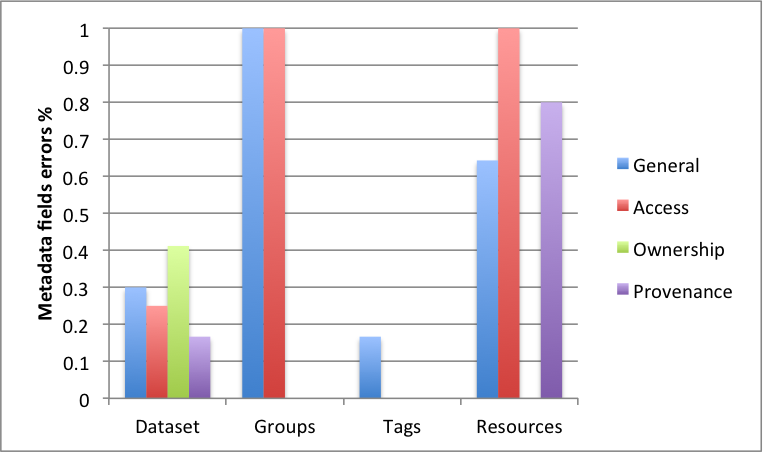
\includegraphics[width=.95\linewidth]{metadata_noise_by_section.png}
\captionsetup{textfont=small,singlelinecheck=off,justification=centering}
\caption{Error \% by section}
\label{fig:2}}
\qquad
\begin{minipage}{7cm}\hspace*{-.6in}
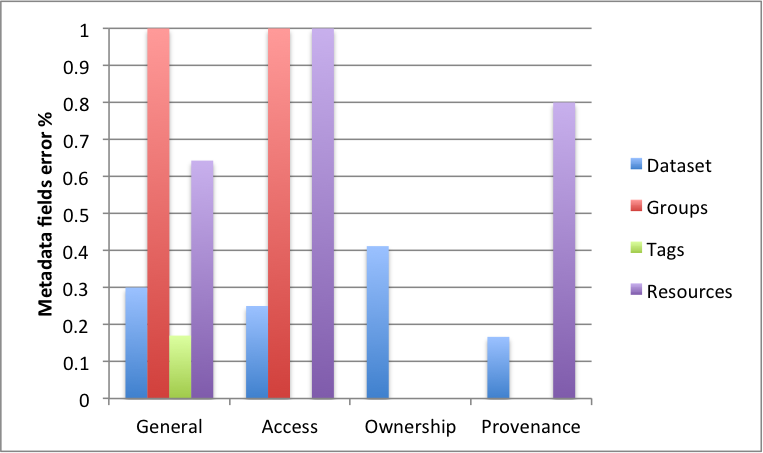
\includegraphics[width=.95\linewidth]{metadata_noise_by_metadata_type.png}
\captionsetup{textfont=small,singlelinecheck=off,justification=raggedright}
\caption{Error \% by information type}
\label{fig:3}
\end{minipage}

\end{figure}

We notice that 42.85\% of the top metadata problems can be fixed automatically. 44.44\% of these problems can be fixed by our tool while the others need tools that are plugged into the data portal. We further present and discuss the results grouped by metadata information type below.

\subsection{General information} 34 datasets (13.13\%) did not have valid \texttt{notes} values. \texttt{tags} information for the datasets were complete except for the \texttt{vocabulary\_id} as it was missing from all the datasets' metadata. All the datasets \texttt{groups} information were missing \texttt{display\_name, description, title, image\_display\_url, id, name}. After manual examination, we noticed a clear overlap between group and organization information. Many datasets like \texttt{event-media} used the organization field to show group related information (being in LOD Cloud) instead of the publishers details.\\

\subsection{Access information} 25\% of the datasets access information (being the dataset URL and any URL defined in its groups) has issues related to them (missing or unreachable URLs).
Three datasets (1.15\%) did not have a URL defined (tip, uniprot\-databases, uniprot\-citations) while 45 datasets (17.3\%) defined URLs were not accessible at the time writing this paper. One dataset did not have resources information (bio2rdf\-chebi) while the other datasets had a total of 1068 defined resources.\\
On the datasets resources level, we noticed wrong or inconsistent values in the \texttt{size} and \texttt{mimetype} fields. 20 (1.87\%) resources had incorrect \texttt{mimetype} defined, while 52 (4.82\%) had incorrect \texttt{size} values. These values have been automatically fixed based on the values defined in the HTTP response header. However, 44 datasets have valid \texttt{size} field values and 54 have valid \texttt{mimetype} field values where they were not reachable, thus providing incorrect information.\\
15 (68\%) fields of all the other access metadata are missing or have undefined values. Looking closely, we noticed that most of these problems can be easily fixed automatically by tools that can be plugged to the data portal. For example, the top six missing fields are the \texttt{cache\_last\_updated}, \texttt{cache\_url}, \texttt{url\-type}, \texttt{webstore\_last\_updated}, \texttt{mimetype\-\_inner} and \texttt{hash} which can be computed and filled automatically. However, the most important missing information which require manual entry are the dataset's \texttt{name} and \texttt{description} were missing from 817 (76.49\%) and 98 (9.17\%) resources respectively.
A total of 334 resources (31.27\%) URLs were not reachable, thus affecting highly the availability of these datasets. CKAN resources can be of various predefined types $(file, file.upload, api, visualization, code and documentation)$. The frameowork also breaks down these unreachable resources according to their types. 211 (63.17\%) resources did not have valid \texttt{resource\_type}, 112 (33.53\%) were files, 8 (2.39\%) and one (0.029\%) metadata, example and documentation types.

To have more details about the resources URL types, we created a $key:object meta-field values$ group level report on LOD cloud with \texttt{resources>format:title}. This will aggregate the resources format information for each dataset. We found out that only 161 (62.16\%) of the datasets valid URLs have SPARQL endpoints defined by \texttt{api/sparql} resource format. 92.27\% provided RDF example links and 56.3\% provided direct links to RDF down-loadable dumps.

The noisiest part of the access metadata was license information. A total of 43 datasets (16.6\%) did not have a defined \texttt{license\_title} and \texttt{license\_id} fields, where 141 (54.44\%) had missing \texttt{license\_url} field. However, we managed to normalize 123 (47.49\%) of the datasets' license information using the manual mapping file.

\subsection{Ownership information} Ownership information is divided into direct ownership (author and maintainer) and organization information. Four fields (66.66\%) of the direct ownership information were missing or undefined. The breakdown for the missing information is: 55.21\% \texttt{maintainer\_email}, 51.35\% \texttt{maintainer}, 15.06\% \texttt{author\_email}, 2.32\% \texttt{author}. Moreover, our framework performs checks to validate existing email values. 11 (0.05\%) and 6 (0.05\%) of the defined \texttt{author\_email} and \texttt{maintainer\_email} fields were not valid email addresses respectively.\\
For the organization information, two field values (16.6\%) were missing or undefined. 1.16\% of the \texttt{organization\_description} and 10.81\% of the \texttt{organization\-\_image\_url} information with two out of these URLs were unreachable.

\subsection{Provenance information} 80\% of the resources provenance information were missing or undefined. However, most of the provenance information e.g. \texttt{metadata\_created, metadata\_modified)} can be computed automatically by tools plugged into the data portal. The only field requiring manual entry is the \texttt{version} field which was found to be missing from 60.23\% of the datasets.

%%%%%%%%%%%%%%%%%%%%%%%%%%%%%%%%%%%%%%%
%%%  5. Conclusion and Future Work  %%%
%%%%%%%%%%%%%%%%%%%%%%%%%%%%%%%%%%%%%%%
\section{Conclusion and Future Work}
\label{sec:conclusion}

In this paper, we proposed a scalable automatic approach for extracting, validating, correcting and generating descriptive linked dataset profiles. This approach applies several techniques in order to check the validity of the metadata provided and to generate descriptive and statistical information for a particular dataset or for an entire data portal. Based on our experiments running the tool on the LOD cloud, we discovered that the general state of the datasets needs attention as most of them lack informative access information and their resources suffer low availability. These two metrics are of high importance for enterprises looking to integrate and use external linked data.\\
It has been noticed that the issues surrounding metadata quality affect directly dataset search as data portals rely on such information to power their search index. We noted the need for tools that are able to identify various issues in this metadata and correct them automatically. We found out that 32.25\% of all the metadata information can be automatically fixed, on which 50\%of them can be directly fixed by our framework. The rest are mainly provenance information that requires special treatment.\\
As part of our future work, we plan to introduce workflows that will be able to correct the rest of the metadata either automatically or through intuitive manually-driven interfaces. We also plan to integrate statistical and topical profilers to be able to generate full comprehensive profiles. We also intend to suggest a ranked standard metadata model that will help generate more accurate and scored metadata quality profiles. We also plan to run this tool on various CKAN based data portals, schedule periodic reports to monitor the evolvement of datasets metadata. Finally, at some stage, we plan to extend this tool for other data portal types like DKAN and Socrata.

\chapter{Hybrid Event Recommendation}    \label{ch:recommendation}
\graphicspath{{Part2/Chapter2/figures/}}

Recommendation in online services has gained momentum during the recent past years as a key factor to deliver personalized content. Reducing the information overload and assisting customers to make decision become part of primary concerns in the e-service area. To this aim, recommender systems attempt to provide efficient filters that decode the user interests, and optimize accordingly the information perceived. To help these systems predict items of interest, various clues are available ranging from a user profile, explicit ratings, to past activities and social interactions. For more details, Appendix~\ref{app:recommendation} describes two popular recommendation techniques, namely the content-based recommendation and the collaborative filtering.

Integrating a recommender system in event-based services is a key advantage to attract people attending events and to promote face-to-face social interactions. Indeed, the event recommendation can draw on different features such as the user preferences (ratings, likes, etc.), the attended events (visited places, involved artists), or even the social co-participation. Broadly speaking, the decision making upon attending events depends on some restrictions such as time, location, category, popularity and which friend will attend. However, the existing techniques (e.g. collaborative filtering and content-based methods) cannot cope at all with the complex inherent nature of such decision. In addition, a recommender system is often application-specific, that is, to be tuned according to the item context (e.g. type, reasons to select an item, etc.). Another challenge in our work is that events often involve different topics (e.g. different genres in one musical concert). As a result, the user profile constructed based on the attended events may contain a wide variety of topics. This leads to topically diverse profile that may conceal the effective user interests. 

To tackle these issues, we propose a hybrid recommender system based on Semantic Web technologies~\cite{Khrouf:RecSys2013}. Our belief is that a structured representation presents one solution to cope with the complexity of event-specific characteristics. This modeling will ensure a more straightforward way to explore and reason over the data. It makes possible to ask complex queries, for example, to retrieve events involving the same artist within a specific geographical area. In addition, the semantic model empowers the enrichment of event descriptions with additional information from Linked Data. Such enrichment can provide valuable inputs for the content-based recommender system~\cite{DiNoia:SEMANTICS12}.

In the second step of our approach, we propose to quantify the user interests based on topic modeling technique. The objective is to detect the user propensity towards specific topics. It will be integrated in the recommender system in order to control the impact caused by the diversity of a user profile. Finally, we exploit the collaborative participation assuming that the social information about ``which friend will attend an event'' plays an important role in decision making. In this work, we mainly investigate the extent to which the data enrichment, the social information and the user interests modeling can improve the system performance.


\section{Content-based Recommendation using Linked Data}
\label{sec:linkeddata-recommendation}
The principle of content-based (CB) recommendation is to suggest new items similar to those a user liked in the past. The similarity between items is computed based on the descriptive features of the item using a distance measure such as Cosine similarity, Pearson correlation and Latent Semantic Analysis~\cite{Landauer:1998}. The most common representation of the item is the keyword-based model, in which attributes are represented by weighted vectors of keywords usually computed by TF-IDF scheme (term frequency/inverse frequency). To build such a profile from unstructured data, feature extraction techniques are needed to shift the item description from the original representation to a structured form suitable for next processing (e.g. keyword vectors). This task becomes straightforward by the use of Semantic Web technologies. CB recommender systems can greatly benefit from the ease of ontology-enabled feature extraction, and the availability of Linked Data covering different domains to enrich the item profile. In the following, we explain how to compute the items similarity in Linked Data.

\subsection{Items Similarity in Linked Data}
In order to compute the similarity between items in Linked Data, we resolved to apply the approach proposed by Di Noia et al~\cite{DiNoia:SEMANTICS12}. The key idea is that semantically similar items from RDF graph are the subject of two RDF triples having the same property and the same object (where a triple=$<$subject,property,object$>$). The intuition behind is that: \textit{if two subjects are in the same relation to the same object, this is evidence that they may be similar subjects}. Technically, the approach is based on an adaptation of the classic Vector Space Model (VSM)~\cite{Salton:CACM75}, a well-known technique in Information Retrieval (IR). In this model, similarity between documents and queries is computed using their representative t-dimensional weighted vectors of discriminating terms. The application of VSM in RDF graph projects the Linked Data to 3-dimensional tensor where each slice represents an adjacency matrix corresponding to one property in the ontology. Indeed, the Linked Data network can be defined as a graph $G=(V,E)$ where $V$ is a set of resources and $E$ is the set of properties between resources in $V$. For each property $p$ in the set $E$, the related adjacency matrix presents the linkage between the subjects (on the rows) and the objects (on the columns) from $V$ via $p$. Then, a non null weight is assigned to each entry $X_{i,j,p}$ in the tensor for each existing triple $<i^{th}$ subject, $p^{th}$ property, $i^{th}$ object$>$. Figure~\ref{fig:tensor-slices} shows an example of tensor slices related to some properties, namely: \texttt{lode:atPlace}, \texttt{lode:involvedAgent} and \texttt{dc:subject}.

\begin{figure}
  \centering
  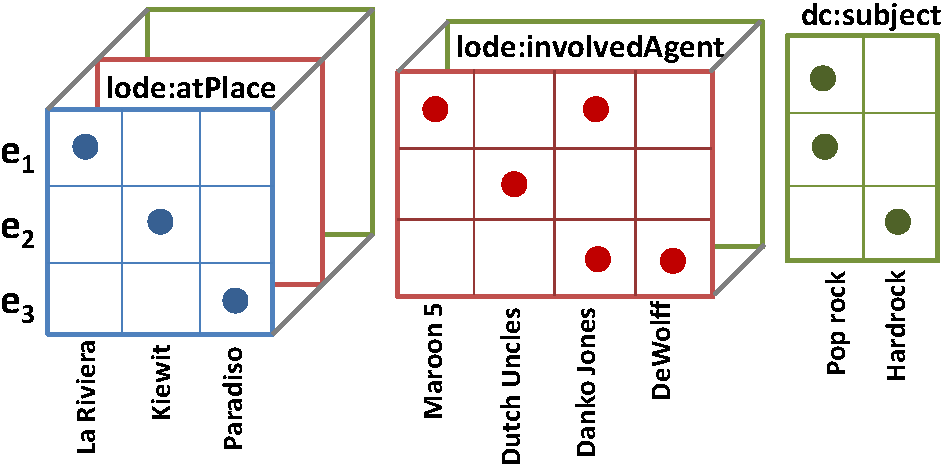
\includegraphics[scale=0.67]{tensor-slices.pdf}
  \caption{Tensor slices of some event properties (place, agent and subject)}
  \label{fig:tensor-slices}
\end{figure}

Assuming that the properties are semantically independent, we would be able to compute the similarity between events according to each property separately. The representation of an event $e_{i}$ according to the property $p$ is a t-dimensional vector indexing the terms/objects related to $e_{i}$ via $p$. The TF-IDF weight of each object $o$ is:

\begin{equation} \label{eq:weight}
w_{o,i,p}=f_{o,i,p} \ \cdot \ log \ \left(\frac {N}{m_{o,p}}\right)
\end{equation}
where $f_{o,i,p} = 1$ if a link exists between the node $e_{i}$ and the object $o$ via the property $p$, otherwise $f_{o,i,p}=0$. $N$ is the total number of events in the dataset, $m_{o,p}$ is the number of events linked to the object $o$ via the property $p$. Then, the similarity between two events $e_{i}$ and $e_{j}$ according to the property $p$ is computed using Cosine distance between their representative vectors as following:

\begin{equation}
sim^{p}(e_{i},e_{j})=\frac {\sum_{r=1}^{t} w_{r,i,p} \cdot w_{r,j,p}} {\sqrt{\sum_{r=1}^{t} w^{2}_{r,i,p}} \cdot \sqrt{\sum_{r=1}^{t} w^{2}_{r,j,p}}}
\end{equation}
This approach can be applied to detect similarity between subjects or objects of RDF triples. It has been successfully used to recommend movies and to improve the quality of content-based system~\cite{DiNoia:SEMANTICS12}. However, it is still limited when the adjacency matrix is very sparse such as the case of matrices associated with \texttt{lode:atPlace} and \texttt{lode:involvedAgent} properties. In fact, such predicates are characterized by the diversity of their object values, thus considered as discriminant properties. For instance, the t-dimensional vector related to \texttt{lode:atPlace} property has only one non-zero weight since an event is typically held at only one venue.


\subsection{Similarity-based Interpolation}

In order to mitigate the sparsity of the adjacency matrix, we propose to interpolate fictitious values based on the similarity between objects. Thus, we initially introduce a discriminability metric (i.e. discriminant power) to gain insight into the properties associated with highly sparse matrices. The metric is defined as following:

\begin{equation}
 Discriminability(p) = \frac{\mid{\{o\mid t=<s,p,o>\ \in G\}}\mid}{\mid{\ t=<s,p,o>\ \in G \mid}}
\end{equation}
where $G$ is the RDF graph, $t$ is the triple representing the link between the subject $s$ and the object $o$ via the property $p$. This formula quantifies the discriminability by the number of different object values on the target property. For instance, from a set of 1700 events (related to 10,323 agents, 627 places and 5,758 subjects), we found a discriminability score of 0.64 for the \texttt{lode:involvedAgent} and 0.45 for the \texttt{lode:atPlace}, while it is only equal to 0.10 for the \texttt{dc:subject} predicate. Furthermore, similar events are not necessary occurred at the same location or featuring the same performers. In order to reduce the discriminability impact, we interpolate fictitious weights in the adjacency matrix based on the similarity between objects as depicted in Figure~\ref{fig:interpolation}. 

\begin{figure}[htb]
  \centering
  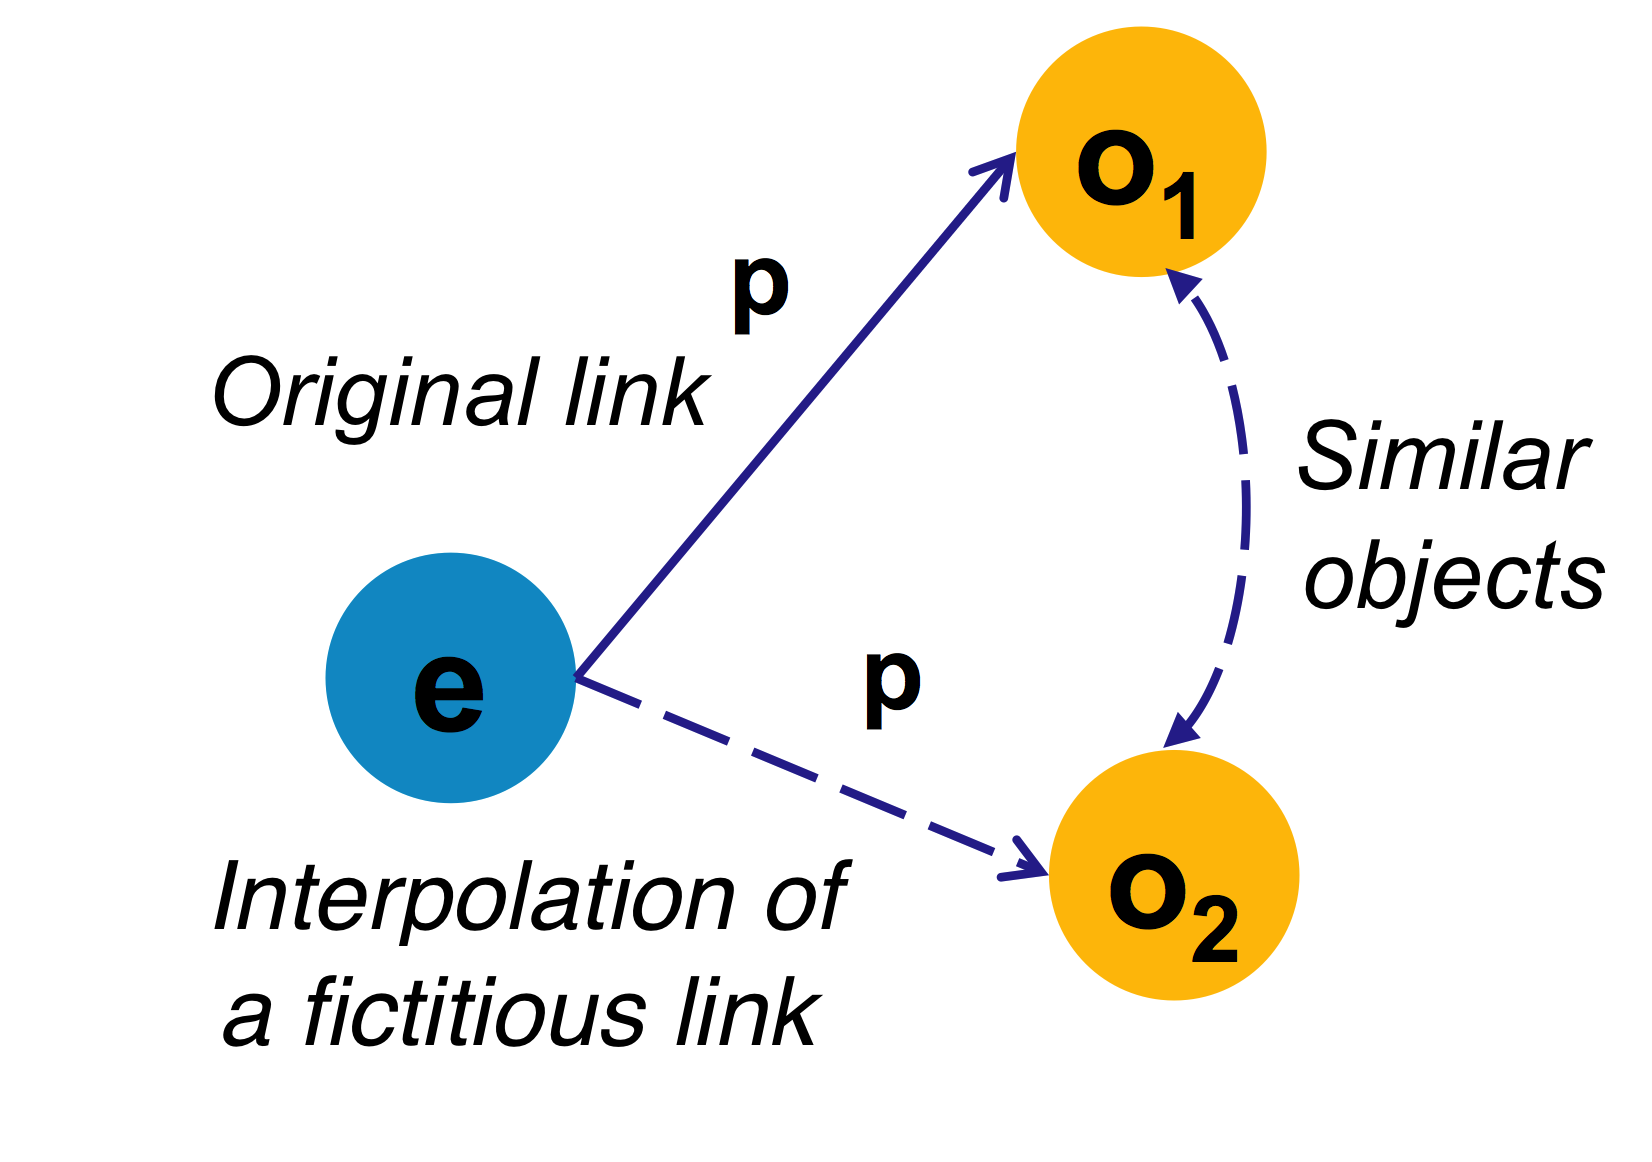
\includegraphics[scale=0.1]{sim-interpolation.png}
  \caption{Similarity-based Interpolation}
  \label{fig:interpolation}
\end{figure}

More precisely, if an object $o_{k}$ is similar to another object $o_{h}$, and if both $f_{o_{h},i,p} = 1$ and $f_{o_{k},i,p} = 0$, then $f_{o_{k},i,p} = sim(o_{k},o_{h})$. Note that $f_{o_{k},i,p}$ reflects the strength of the fictitious link which associates the event $e_{i}$ with the object $o_{k}$ via the property $p$. If the object $o_{k}$ is similar to more than one object originally linked to the event $e_{i}$, the weight $f_{o_{k},i,p}$ will be equal to the highest similarity score. Thus, for each object $o_{k}$, the equation~\ref{eq:weight} becomes:

\begin{equation}
w_{o_{k},i,p}= \max_{o_{h} \in H}sim(o_{k},o_{h}) \ \cdot \ log \ \left(\frac {N}{m_{o_{k},p}}\right)
\end{equation}
where $H$ is the set of objects originally linked to the event $e_{i}$. The intuition behind this formula is that: \textit{if two subjects are in same relations to similar objects, this is evidence that they may be similar subjects}. We do not pay attention to how similarity between objects is computed. In fact, this measure depends on the nature of the object itself and there exist several existing techniques that can be used. In our case, we exploit the similarity scores between agents (i.e. artists) provided by third party services such as Last.fm, and we compute the normalized geographical distance between venues.


%%%%%%%%%%%%%%%%%%%%%%%%%%
%%%  3. Event Recommendation %%%
%%%%%%%%%%%%%%%%%%%%%%%%%%

\section{Event Recommendation }
\label{sec:event-recommendation}
Different from a classic item, events occur at a specific place and during a period of time to become worthless for recommendation. Moreover, while a classic item (e.g. movie, book) continuously receives useful feedback, an event has few rating due to its transiency. In our dataset, these ratings are represented by the binary user-event attendance matrix which has a sparsity rate equal to 98\% (i.e. a set of users attend a very limited number of events). As a solution, one can address event recommendation using CB recommender system that exploits the matching of event attributes with the user profile. This perfectly complies with the constraints considered when it comes to decide whether or not to attend an event. Metadata such as distance, time, topics and artists are important and influential factors in such decision. Still, the CB recommendation might suggest items with a limited diversity and overlook the social information regarding the question ``which friend is going?''. To reduce this gap, we propose to enhance its performance by enriching the content using Linked Data, and by improving the detection of the user interests. Then, we incorporate the social information using Collaborative Filtering (CF) method, thus producing a hybrid recommendation.

%%%%%%%%%%%%%%%%%%%%%%%%%%%%%%%%%%%%%%%%%
%%%  3.1 Content-based Recommendation %%%
%%%%%%%%%%%%%%%%%%%%%%%%%%%%%%%%%%%%%%%%%

\subsection{Content-based Recommendation}
The CB recommender system suggests future events similar to those a user has attended in the past. We assume that there is a sufficient number of past attended events in the user profile to avoid the \textit{cold-start} problem\footnote{The problem to produce good recommendations for new users where nothing is known about their preferences}, which is out of the scope of the present work. In order to predict the participation of the user $u$ to the event $e_{i}$, we combine the similarity values between events as following: 

\begin{equation}\label{eq:rankcb}
rank_{cb}(u,e_{i})= \frac{\sum_{e_{j} \in E_{u}} \sum_{p\in P} \ \alpha_{p}\ sim^p(e_{i},e_{j})}{\mid P \mid\  \cdot \mid E_{u}\mid}
\end{equation}
where $E_{u}$ is the set of past events attended by the user $u$, $P$ is the set of properties shared between two events $e_{i}$ and $e_{j}$, and $\alpha_{p}$ is the weight that reflects the contribution of the property $p$ in the recommendation.

The properties selected to compute the similarity between events are those which are related to the location, subjects (tags) and involved agents (artists). In contrast, the temporal information is not considered in this work and left for future study. Our belief is that temporality could be harnessed to index the recent events in the user profile, thus reducing the computation. Still, there is a need to deeply investigate the impact that the reduction of the user profile has on the system performance. 

\myparagraph{Geographic Closeness}
In recent research study, it has been shown that users generally tend to attend nearby entertainment events~\cite{Quercia:ICDM10}. This fact makes the location a valuable feature in event recommendation. In our approach, we need to measure the similarity between events according to the \texttt{lode:atPlace} property. Thus, we normalize the distance between two locations using a specific threshold $\theta$ which needs to be determined. As the user home is missing in our data, we measure the distance between attended events for each user as depicted in Figure~\ref{fig:attendance-distance}. Note that the attendance rate becomes extremely low from $\theta=80$ Km. We consider that this value is the normalization threshold from which the similarity between events is equal to zero according to the \texttt{lode:atPlace} property.

\begin{figure}[H]
  \centering
  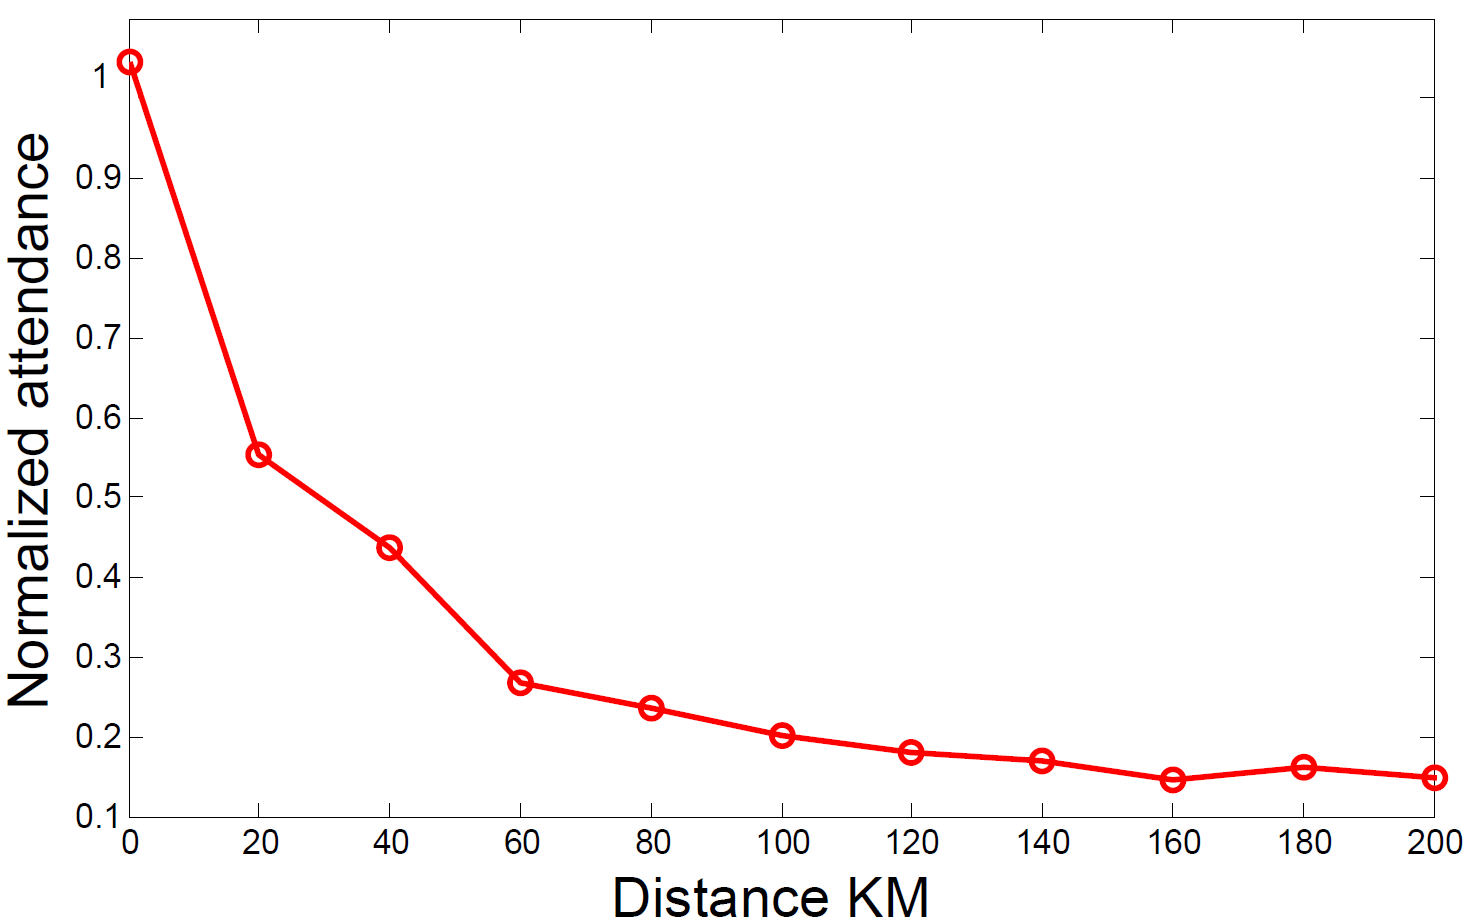
\includegraphics[scale=0.22]{attendance-distance.png}
  \caption{Normalized average attendance per distance}
  \label{fig:attendance-distance}
\end{figure}

\myparagraph{Enrichment with Linked Data} One method to enrich the item profile from Linked Data is to consume background information from DBpedia. The key advantage of DBpedia is the availability of semantically rich data in various domains. Using the mapping between EventMedia and DBpedia, we enrich the topics of an event using the DBpedia topics (e.g. genres) related to the involved artists. More precisely, we retrieve the categories associated with the property \texttt{dcterms:subject} of artists by simply querying the DBpedia SPARQL endpoint\footnote{\url{http://dbpedia.org/sparql}}. The reason behind our interest in DBpedia is that topics are accurately labeled and classified.

\subsection{User Interests Modeling}
One fundamental goal in the recommender system is to suggest new items that best fit the user interests. In our case, this is particularly difficult to achieve due to the presence of topically diverse events. In fact, the real-world social events can be classified into large set of categories ranging from large festivals and conferences to small concerts and social gatherings. When attending an event, the user might be interested in a specific show or artist or might have broad interests. In consequence, relying on event similarity according to the \texttt{dc:subject} property can be influenced by the topical diversity of tags related to events in the user profile. To alleviate this impact, we leverage the Latent Dirichlet Allocation (LDA)~\cite{Blei:MLR03} for detecting the relevant user interests as previously described in Section~\ref{sec:user-interest}.

\begin{figure}[htb]
  \centering
  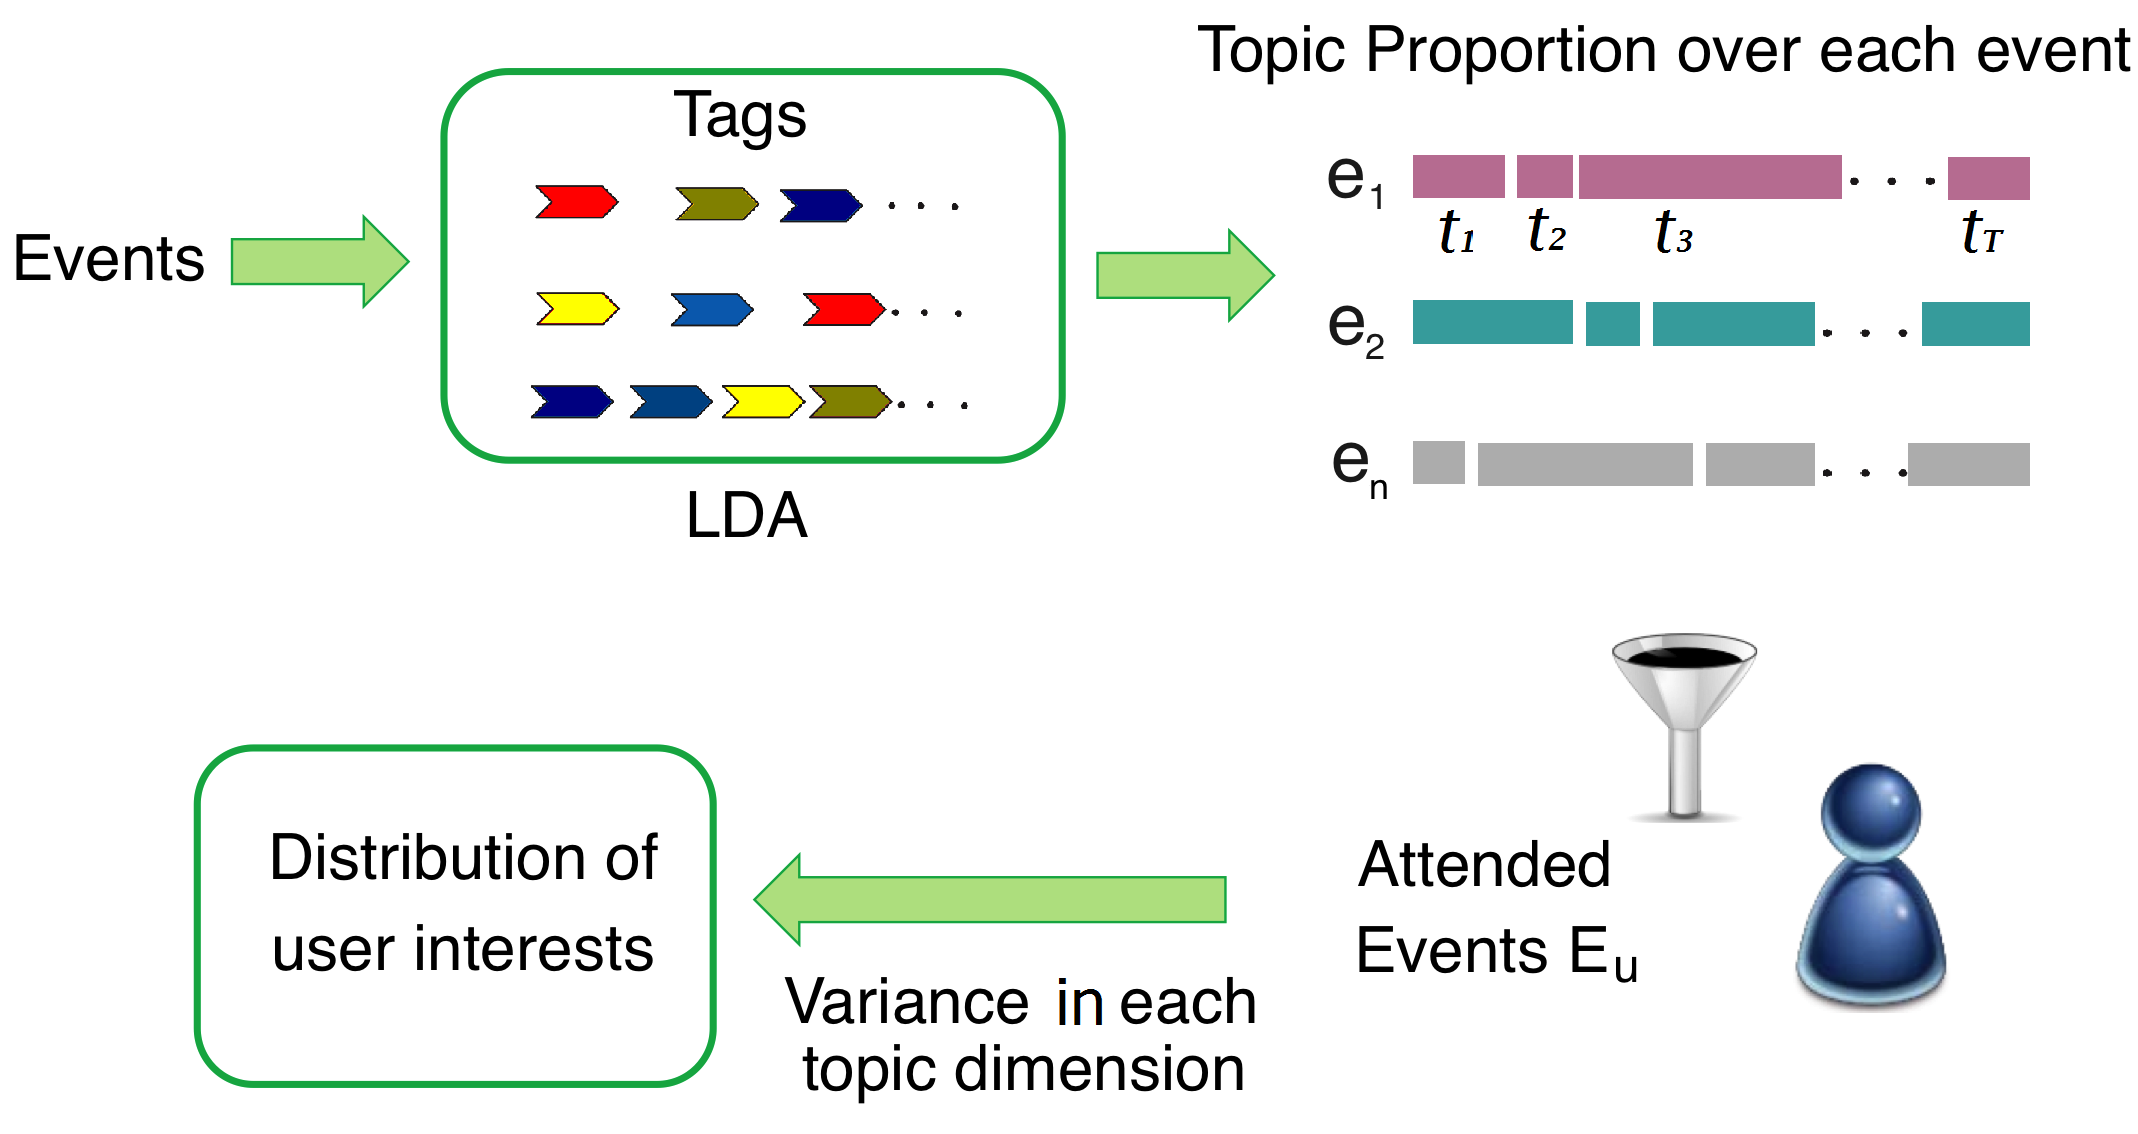
\includegraphics[scale=0.2]{user-div.png}
  \caption{The pipeline of user Interests modeling}
  \label{fig:div-approach}
\end{figure}

Figure~\ref{fig:div-approach} illustrates the pipeline of the user interests modeling. For each event $e_{i}$ having a set of tags, LDA generates a $T$-dimensional vector of topic proportions $\Theta_{i} = [\theta^{1}_{i},\theta^{2}_{i},...\theta^{T}_{i}]$, where $T$ is the number of topics and $\Theta_{i}$ reflects the semantic categories of the event. Then, we compute the variance in each topic dimension $t$ over all the events $E$ attended by a user $\Theta^{t} = [\theta^{t}_{1},\theta^{t}_{2},...\theta^{t}_{E}]$. The diversity score of each corresponding user is the mean of the variances of all the topics dimensions (mean of $\Theta^{1},\Theta^{2}...\Theta^{T})$. 

This approach as introduced by Wu et al.~\cite{Hao:AHJ12} has been originally designed to study the diverseness of individual tastes. But, we think that it is also helpful to detect user's propensity from a topically diverse profile. Indeed, events can be divided into two classes: those related to very few topics or those related to many topics. We consider that events in the first class are those which really exhibit the user interests. Using the variance, we are able to detect high proportions within topic dimension given that this dimension is likely to also contain low proportions (i.e. events are not regularly distributed over the topics).

As an example, Figure~\ref{fig:diversity-scores} shows the normalized diversity scores obtained from a sample of 1,000 Last.fm users. In Figure~\ref{fig:diversity_a}, it is shown that most of diversity scores range from $0.3$ to $0.5$ indicating that users have relatively high interests in specific topics. The diversity scores near to 1 represent users having strong interests in very few topics such as the case of the user plotted in Figure~\ref{fig:diversity_b}. This user has a strong bias specifically towards the topic $9$. Finally, the diversity scores close to zero generally represent the users associated with few attended events (i.e. the cold-start problem).

\begin{figure}[htb]
\centering
\subfigure[]{\label{fig:diversity_a}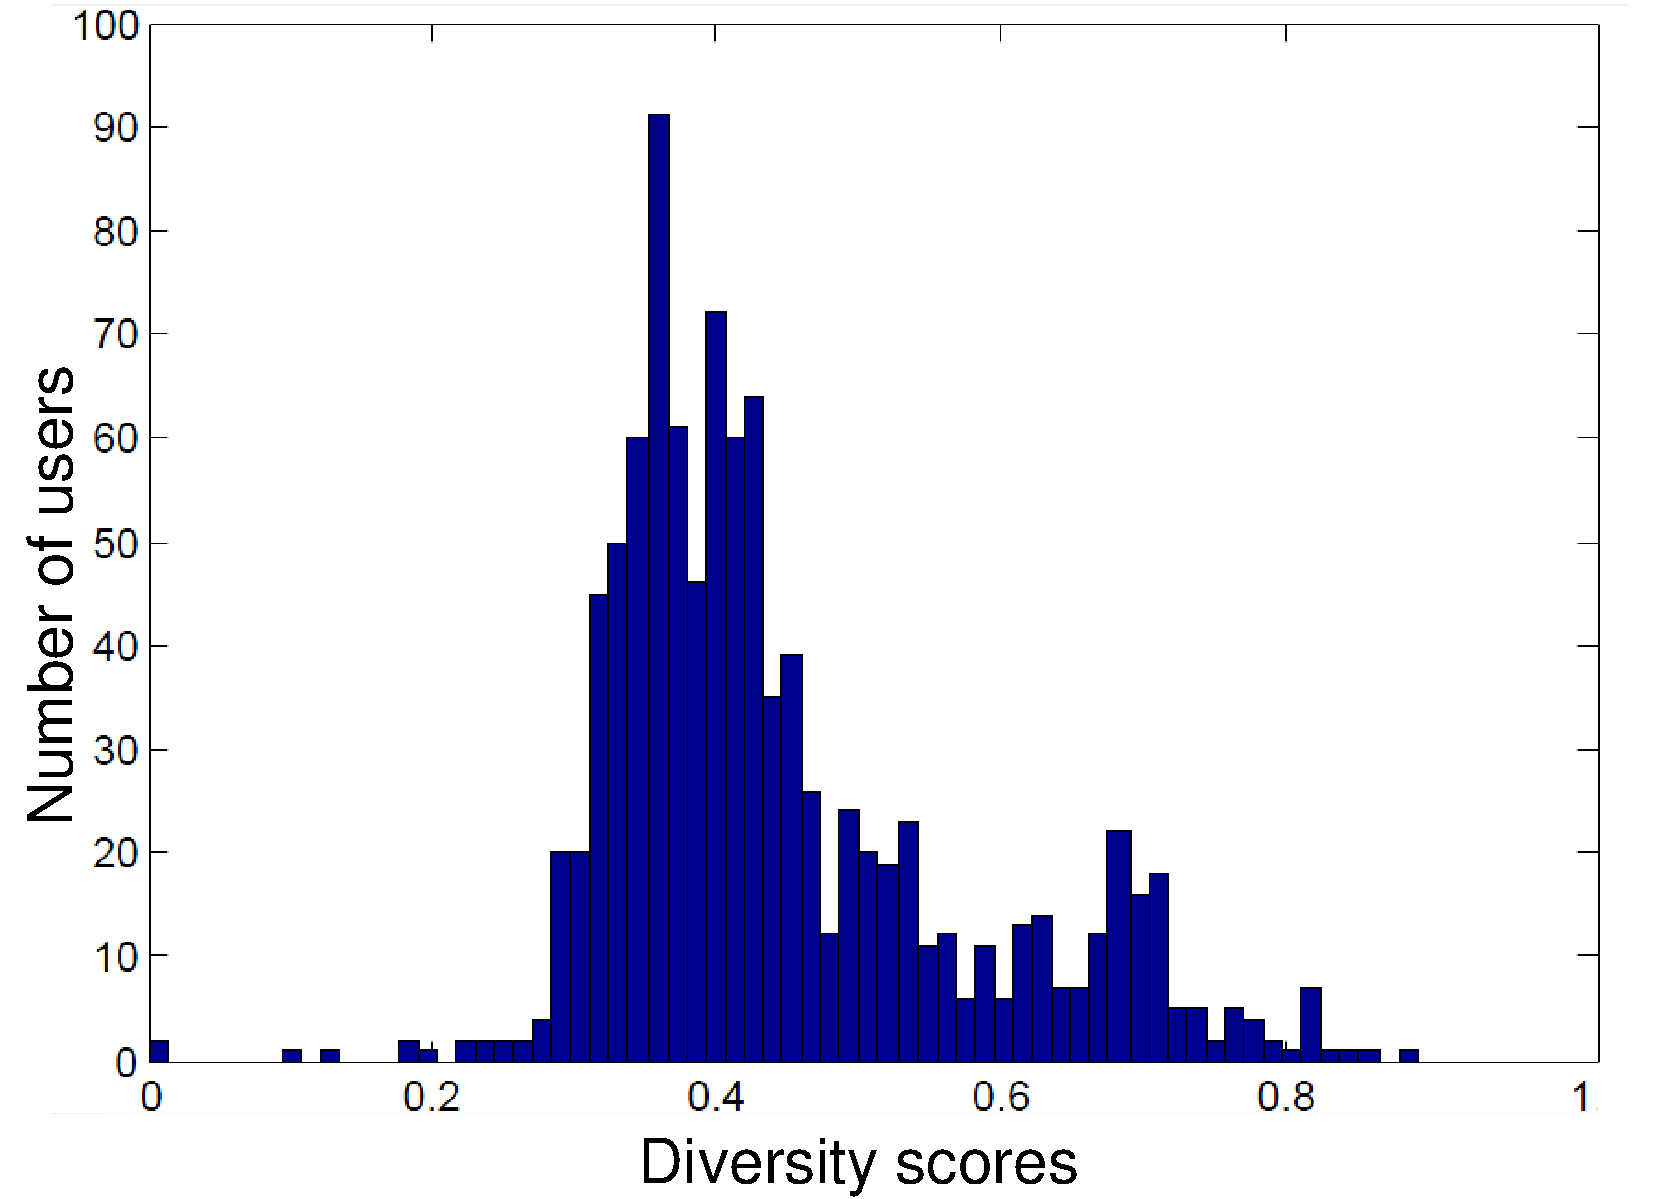
\includegraphics[height=50mm,width=.48\linewidth]{users-diversity.pdf}}
\subfigure[]{\label{fig:diversity_b}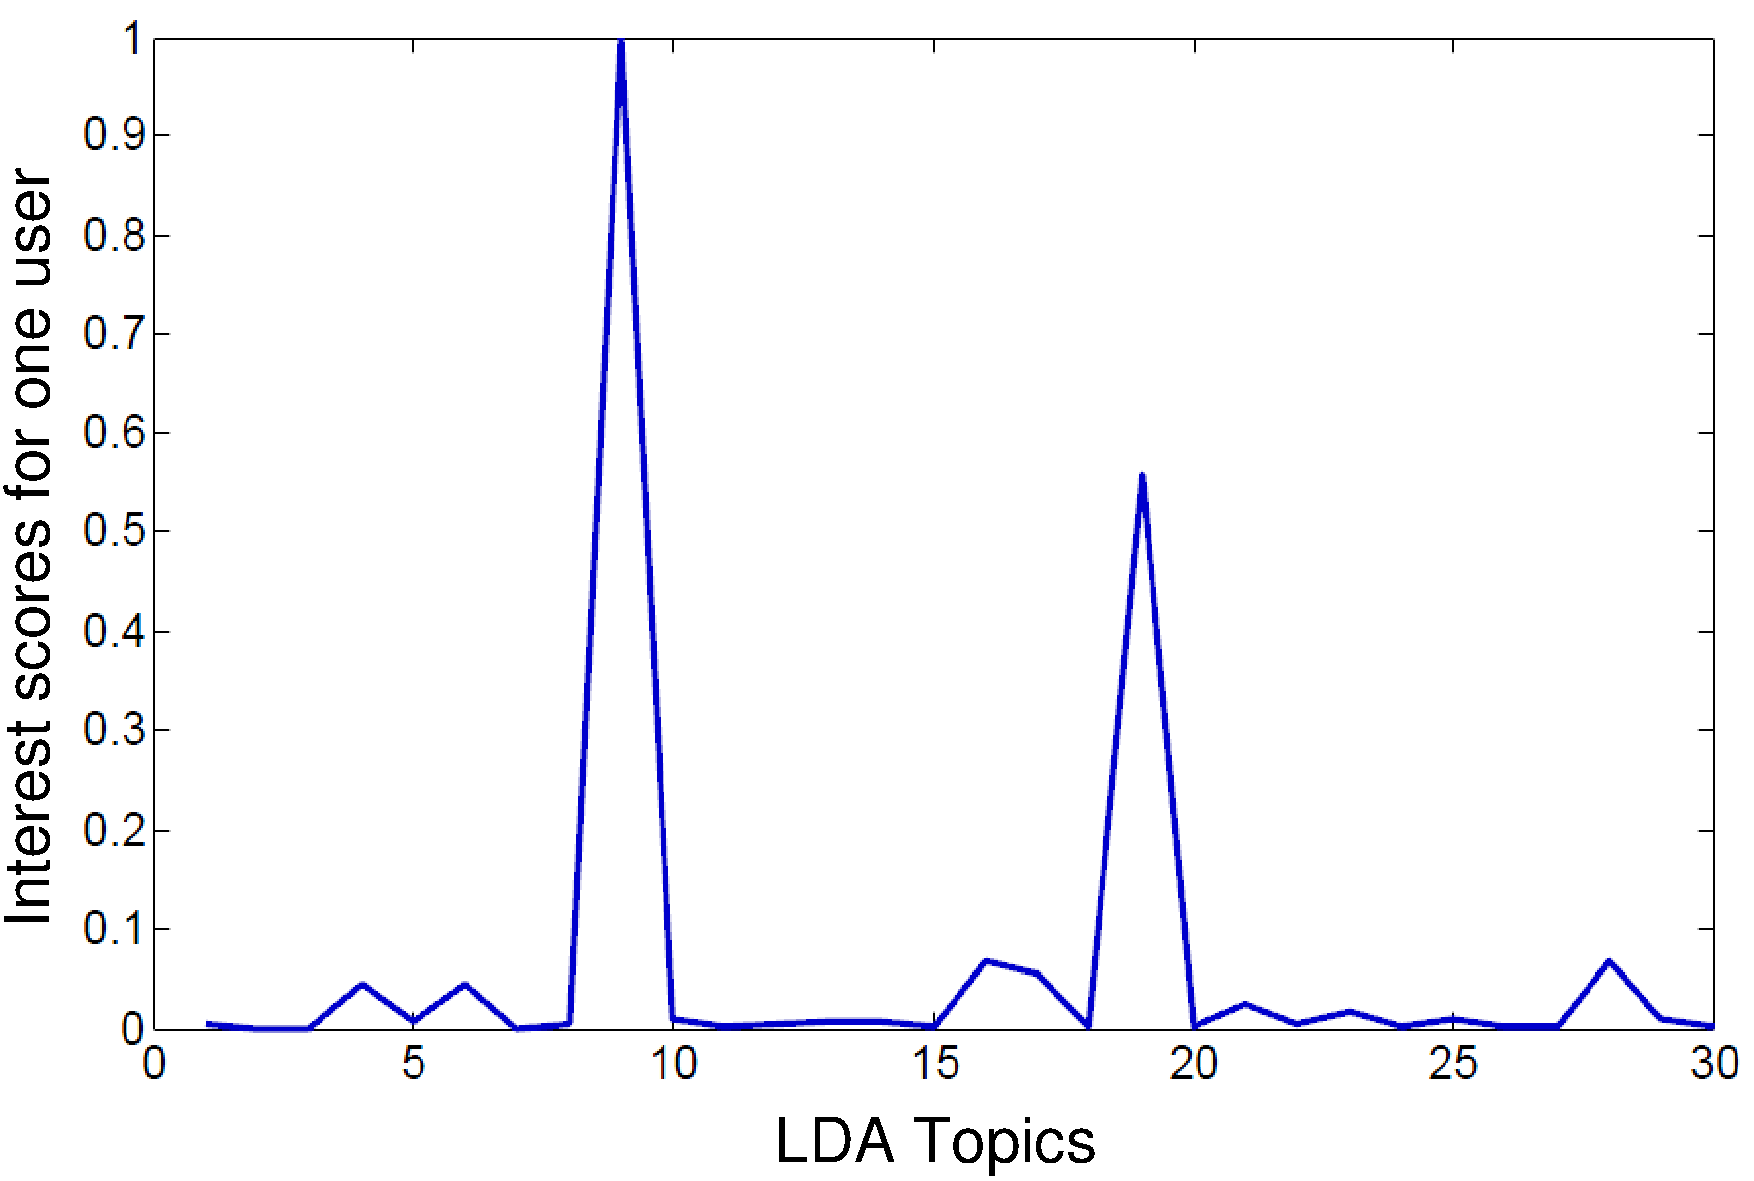
\includegraphics[height=50mm,width=.48\linewidth]{one-user-diversity.pdf}}
\caption{Distribution of topical diversity scores with T = 30: (a) for all the users; (b) for one specific user.}
\label{fig:diversity-scores}
\end{figure}

To take into account the effective user interests in a recommender system, we give emphasis to the events which are more likely to correspond to the user interests. We assign different weights $\beta$ to the events included in the peaks of interest, and to those which are out of these peaks. These weights are then estimated using training methods. The content-based recommendation is extended as following:

\begin{equation}\label{eq:rankcb++}
rank_{cb++}(u,e_{i})= \frac{\sum_{e_{j} \in E_{u}} \sum_{p\in P} \ \alpha_{p}\ \beta_{p} \  sim^p(e_{i},e_{j})}{\mid P \mid\  \cdot \mid E_{u}\mid}
\end{equation}
where $\beta_{p} = 1$ if the property $p$ is different from \texttt{dc:subject}, otherwise the $\beta_{subject}$ is an estimated value depending on whether the event $e_{j}$ corresponds to the user interests or not.


%%%%%%%%%%%%%%%%%%%%%%%%%%%%%%%%%%%%
%%%  3.3 Collaborative filtering %%%
%%%%%%%%%%%%%%%%%%%%%%%%%%%%%%%%%%%%

\subsection{Collaborative Filtering}
A form of social interactions is the collaborative participation such as co-authoring a paper or co-attending an event. In~\cite{Liu:KDD12}, Liu et al. highlight the existence of an offline social network built from the co-attendance of social events. Accordingly, we consider that two users involved in the same event can potentially have a stronger tie than other users. Our assumption is that the more events in which users involve, the stronger is their tie. Thus, the co-attendance can be a clue to provide information at first glance about which ``friends'' will attend an event. Moreover, our dataset contains the users' RSVP that express their intent to join social events, which can be exploited to predict unknown intents. However, unlike the traditional user-based collaborative filtering (CF), we decide to not only consider the similarity between users, but also the contribution of a group of friends. We define the following formula as the prediction that a user $u_{i}$ will attend an event $e$ based on the RSVP of his/her co-attendees (i.e. users who have attended past events with the user $u_{i}$):


\begin{equation}\label{eq:rankcf}
rank_{cf}(u_{i},e)= \frac{\sum_{j \in C } \ a_{i,j}}{\mid C \mid } \ \cdot \  \frac{\mid E_{i} \cap ( \cup_{j \in C } E_{j}) \mid}{\mid E_{i} \mid}
\end{equation}
where $C$ is the set of co-attendees who will attend the event $e$, $E_{i}$ is the set of attended events by the user $u_{i}$, and $a_{i,j}$ is the fraction of common events between the users $u_{i}$ and $u_{j}$ by the cardinality of $E_{j}$. Note that the weight $a_{i,j}$ reflects whether the most of events which are attended by the user $u_{j}$ are also attended by the user $u_{i}$. The rationale behind this formula is two-fold: (1) in the first part, we consider the contribution of each co-attendee individually; (2) in the second part, we consider the co-attendees as a group of friends, and we assume that the more events they attended together with the user $u_{i}$, the more strongly is their relationship.

%%%%%%%%%%%%%%%%%%%%%%%%%%%%%%%%%%
%%%  3.4 Hybrid Recommendation %%%
%%%%%%%%%%%%%%%%%%%%%%%%%%%%%%%%%%

\subsection{Hybrid Recommendation}
To combine the predictions of both CB and CF recommender systems, we propose a weighted hybridization using a linear combination of predicted rank. Taking into account the user diversity and combining the equations (\ref{eq:rankcb++}) and (\ref{eq:rankcf}), we proposed the following function:

\begin{equation}\label{eq:hybrid}
rank(u,e)= rank_{cb++}(u,e) + \ \alpha_{cf}\ rank_{cf}(u,e)
\end{equation}
where $\alpha_{cf}$ is the weight of CF method estimated in conjunction with the weights of CB features using optimization functions for training the system.


%%%%%%%%%%%%%%%%%%%%%%
%%%  5. Evaluation %%%
%%%%%%%%%%%%%%%%%%%%%%

\section{Evaluation}
\label{sec:evaluation}
In this section, we carry out a set of experiments measuring the precision and recall metrics to assess the contribution of each step in our approach, and to evaluate the performance of our system compared with existing approaches.

%%%%%%%%%%%%%%%%%%%%%%%%%%%%%%%
%%%  5.1 Real World Dataset %%%
%%%%%%%%%%%%%%%%%%%%%%%%%%%%%%%

\subsection{Real-world Dataset}
We use the EventMedia dataset and particularly the Last.fm directory which contains a large number of active users. Using SPARQL, we collected 2,436 events, 481 active users whose the attendance rates are within [15,50], generating 12,729 distinct consumption (i.e. user-event pairs). This set of events are related to 14,748 distinct artists, 897 locations and 4265 tags (music domain). For the evaluation, we use a test set containing the most recent 30\% of the consumption and a training test with the remaining 70\% consumption. Then, we measure two metrics used in top-N recommendation task: Precision is the ratio of correctly recommended items and the length of the recommendation $N$; Recall is the ratio of correctly recommended items and the total number of future consumption. Precision and Recall are computed at different $N$ values.

%%%%%%%%%%%%%%%%%%%%%%%%%%%%%%%%%
%%%  4. Learning Rank Weights %%%
%%%%%%%%%%%%%%%%%%%%%%%%%%%%%%%%%

\subsection{Learning Rank Weights}
\label{sec:learning}
To learn the weights of our prediction function, we first test the linear regression with gradient descent that minimizes the least-squares cost function. Then, we use two evolutionary computation methods, namely the Genetic Algorithm (GA) and the Particle Swarm Optimization (PSO) motivated by their success in a wide range of tasks (details in Appendix~\ref{app:optimization}).

%%% Genetic Algorithm %%%

To apply GA in our approach, a chromosome is represented by a vector of the coefficients that need to be estimated. Each chromosome is then evaluated using a fitness function. This function aims to minimize the prediction error and thus maximize the precision of results. Table~\ref{tab:ga-param} shows the GA setting parameters.

\begin{table}[H]
\centering{
\begin{tabular*}{11cm}{c @{\extracolsep{\fill}} ccc}
\hline
Population size & Iterations & crossover & mutation  \\
\hline
30 & 80 & 0.9 & 0.01  \\
\hline
\end{tabular*}
\caption{Setting of GA parameters for event recommendation}
\label{tab:ga-param}
}
\end{table}


%%% Particle Swarm Optimization %%%

As for PSO, a particle is represented by a vector of weights and the fitness function aims at maximizing the precision. Table~\ref{tab:pso-param-2} shows the PSO setting parameters.

\begin{table}[H]
\centering{
\begin{tabular*}{11cm}{c @{\extracolsep{\fill}} cccc}
\hline
Population size & Iterations & $c_{1}$ &  $c_{2}$ & inertia   \\
\hline
30 & 80 & 1.494 & 1.494 & 0.729\\
\hline
\end{tabular*}
\caption{Setting of PSO parameters for event recommendation}
\label{tab:pso-param-2}
}
\end{table}


\subsection{Experiments}
First, we show in Table~\ref{tab:sparsity-tab} the sparsity rates of similarity matrices according to each property. We can see the efficiency of our method to discover latent similarity between events especially for discriminant properties. This highlight the importance of the similarity-based interpolation and the enrichment using Linked Data. Unlike the keyword-based recommender systems, the interpolation is straightforward in our system thanks to the ontology-based data representation.

\begin{table}[H]
\centering{
\begin{tabular*}{8cm}{c @{\extracolsep{\fill}} ccccc}
\hline
Task & location & agent & subject \\
\hline
   (1) & 0.9942 & 0.9174 & 0.3175 \\
\hline
   (2) & 0.6854 & 0.7392 & 0.2843 \\
\hline
\end{tabular*}
\caption{Sparsity rates of the similarity matrices before (1) and after (2) the similarity-based interpolation (for location and agent) and data enrichment with DBpedia (for subject)}
\label{tab:sparsity-tab}
}
\end{table}

Second, we assess the performance of the training methods to learn the coefficients $\alpha$ in the hybrid recommendation algorithm. Note that for this experiment, we do not include the user interests model and we set the $\beta_{subject}$ equal to 1. This experiment aims to rather compare the performance of optimization methods. 

\begin{figure}[htb]
  \centering
  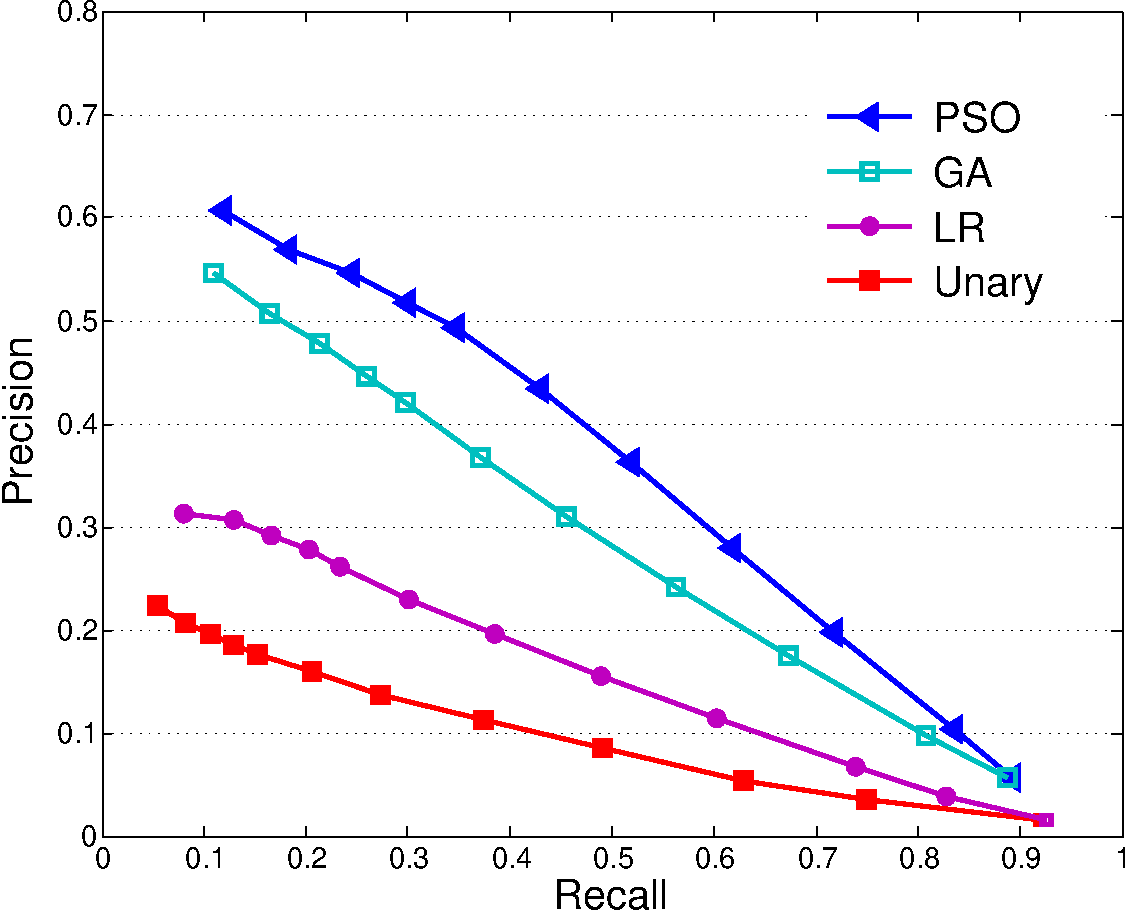
\includegraphics[height=62mm,width=80mm]{training-comparison.pdf}
  \caption{Recall and Precision using different approaches to estimate the vector $\alpha$}
  \label{fig:training-comparison}
\end{figure}

Figure~\ref{fig:training-comparison} shows the Precision and Recall curves. It is obvious that setting all the coefficients equal to 1 achieves the worst performance because there is no adaptive optimization. It is also shown that precision optimization methods (GA and PSO) yield considerably better results compared with error (RMSE) minimization method based in linear regression. This has been also proved in recent work~\cite{Cremonesi:RecSys10} showing that methodologies based on error metrics do not necessarily improve the accuracy of top-N recommendation task. One given explanation is that the RMSE-oriented methods rely only on known ratings to train the system and do not consider the unrated items. Finally, Figure~\ref{fig:training-comparison} highlights the better performance of PSO compared with GA algorithm. We observed a faster convergence to the optimal solution in PSO compared with GA which needs more iterations. This is due to the inherent behavior of PSO where the evolution is only guided by the best particle. In contrast, the GA evolution is guided by a group of solutions in which even weak candidates continue to survive after some iterations. In the following, we use the PSO algorithm to train the system.

To gain insight into the influence of the different steps in our approach, we examine the evolution of the system performance by incorporating in each experiment (by order) the enrichment with DBpedia, the user interests model and the collaborative filtering. Results are illustrated in Figure~\ref{fig:case-comparison}. We can observe that enriching data with DBpedia slightly improves both precision and recall. Indeed, introducing more coherent and qualitative data is one solution to reduce the noise that can be found in the collective knowledge of crowd tagging (e.g. Last.fm tags). Then, the user interests modeling also enhances the system performance. For this experiment, we fix the coefficients $\alpha$ obtained with PSO. Then, we train the system to compute the coefficient $\beta_{subject}$ which depends on the peaks of the user interests. As a result, we obtain $\beta_{subject}$ equal to 0.4 when the event is not included in an interest peak, and $\beta_{subject}$ equal to 1.6 (4 times more) otherwise. This proves the importance to clearly discern the user interests when the user profile contains diverse topics. Finally, combining these results with the collaborative filtering notably increases the recommendation accuracy. Our belief is such improvement is perfectly tangible with the use of a real-world dataset. According to the user centered study presented by Fialho et al.~\cite{Fialho:EVENTS10}, social information such as people and friends who are attending an event has strong priority and influence on decision making.

\begin{figure}[H]
  \centering
  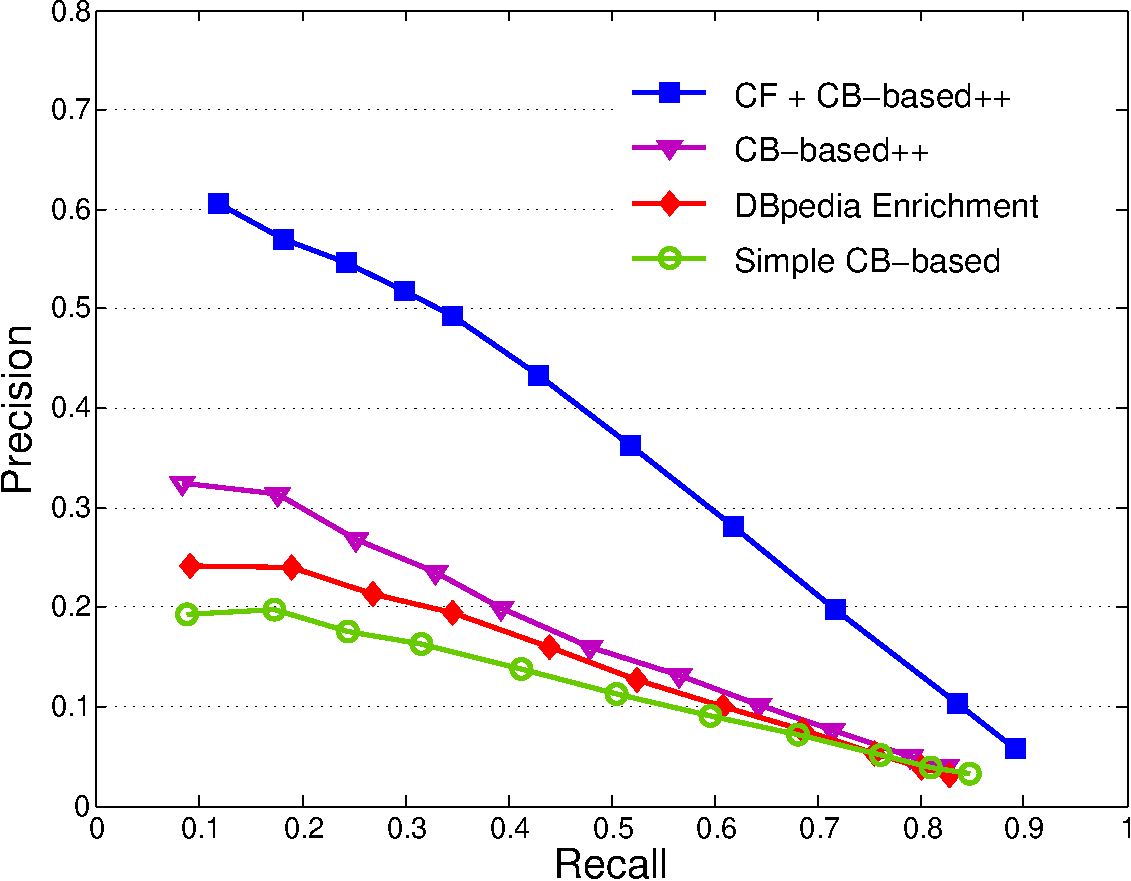
\includegraphics[height=62mm,width=80mm]{case-comparison.pdf}
  \caption{Evolution of the recommendation accuracy by incorporating the DBpedia enrichment, user diversity (CB-based++) and collaborative filtering (CF) }
  \label{fig:case-comparison}
\end{figure}

Lastly, we assess the extent to which a hybrid event recommendation outperforms the existing collaborative filtering based on matrix factorization to detect latent factors from the user-item matrix. We compare our system with the traditional user-based CF and the Probability based Extended Profile Filtering (UBExtended) proposed by Pessemier et al.~\cite{Pessemier:MTA12} to recommend events. This method employs a cascade of two user-based CF systems aiming to recommend the most consumed (i.e. popular) events. The rationale behind is that the probability to consume an event is proportional to the current popularity of the event (i.e. has attracted many users). The comparison results are depicted in Figure~\ref{fig:approaches-comparison}. It is shown that the UBExtended method outperforms the user-based CF algorithm. Still, the hybrid recommendation exhibits the best results in terms of precision and recall. This is due to the benefits of hybridization as has been highlighted in other research studies~\cite{Rojsattarat:2003}.

\begin{figure}[H]
  \centering
  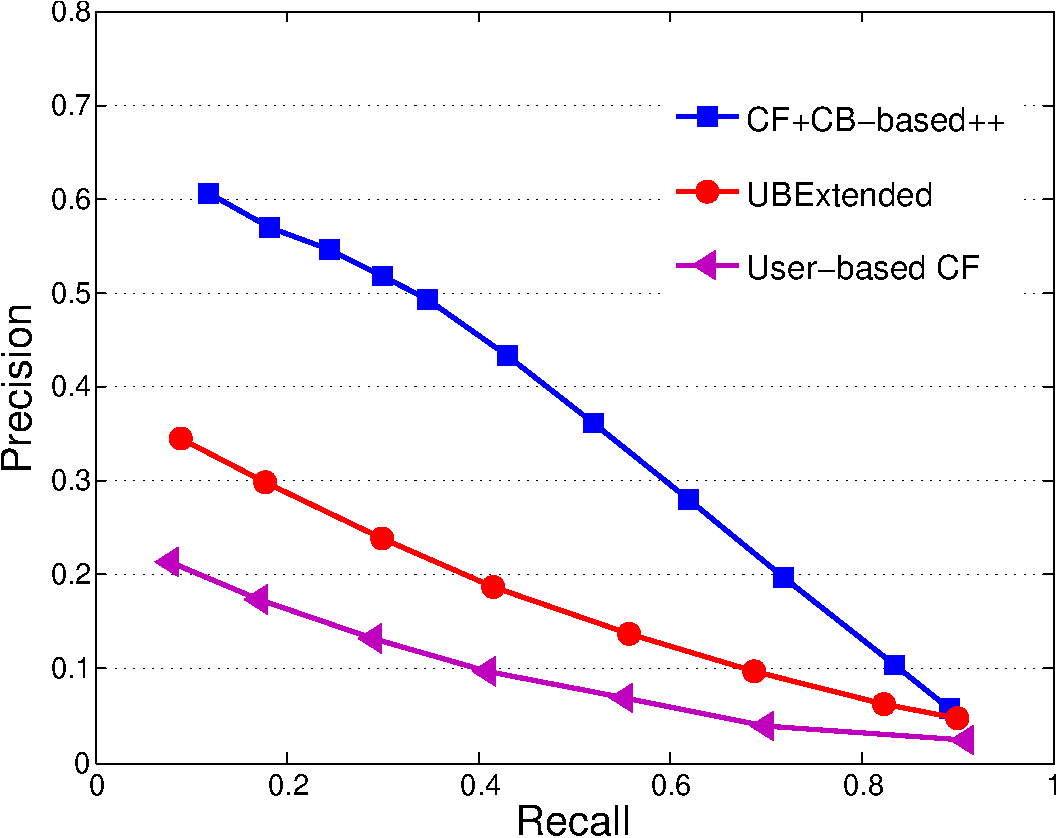
\includegraphics[height=62mm,width=80mm]{approaches-comparison.pdf}
  \caption{Comparison of hybrid event recommendation with pure CF algorithms}
  \label{fig:approaches-comparison}
\end{figure}

\section{Related Work}
\label{sec:related-work}
In the research area of recommender systems, many approaches have been proposed to recommend movies, but few are the studies that deal with event recommendation. Events are particularly hard to recommend due to their short life time and the system often suffers from high sparsity of rating data. Some works have been proposed to overcome these issues and improve the recommendation accuracy. Cornelis et al.~\cite{Cornelis:IICAI05} built a hybrid approach within a fuzzy relational framework that reflects the uncertain information in the domain. The rationale behind is to recommend future events similar to those like-minded users have liked in the past. However, this framework was not evaluated and there is no clear insight about its performance. Minkov et al.~\cite{Minkov:CIKM10} followed the same rationale and proposed a low rank collaborative method to predict the rating of future events. They highlight the performance of the collaborative filtering over the content-based system. Still, their approach was more tailored to recommend scientific talks in the same building and there is no consideration of the geographical constraint. Some other systems have been developed such as ``Pittcult''~\cite{Lee:RecSys08} and ``Eventer''~\cite{Kayaalp:ASONAM09} that position the user within a social network and leverage the trustworthiness between users. Such feature is valuable for recommendation, but it is not available in many systems. Finally, a user centered evaluation~\cite{Dooms:RecSys11} showed that the straightforward combination of CF and CB recommendations outperforms both individual algorithms on almost qualitative metrics such as accuracy, novelty, diversity, satisfaction and trust. Another interesting related works are the recent studies that harness the power of Linked Data in recommender systems. In~\cite{DiNoia:SEMANTICS12}, Di Noia et al. use the Linked Data as the only background knowledge to recommend movies. They highlight the performance of the system that exploits ontology-based data representation compared with the keyword-based representation. Still, there is no deep exploitation of the latent similarity that may exist between movie attributes (e.g. two similar actors).

\section{Conclusion}   \label{sec:conclusion}
In this chapter, we presented an approach for event recommendation combining both CB and CF advantages, and using Linked Data to enrich the event profile. In addition, we proposed an approach to model the user interests and to overcome the topical diversity in the user profile. The evaluation particularly highlights the importance of social information and the user diversity model to enhance the system performance. In the future, we plan to take into account other significant features such as event popularity and temporal indexing of recent consumption.

\chapter*{Conclusion of Part~\ref{pa:part1}}

In this part, we presented the different steps required to build an event-based environment, harnessing the wealth of information provided by different Web services. We used the Semantic Web technologies for connecting the sparse event and media descriptions, so that they become more discoverable and reusable. Overall, we described how the event-centric data has been extracted, converted, interlinked and published following the Linked Data principles.
\\
\\
First, we developed a framework that offers a simple-to-use and flexible tool to scrap events and related media using some popular Web services. Data is continuously feeding EventMedia, a RDF dataset published in the Linked Data cloud. 
\\
\\
Second, we detailed the challenges faced to reconcile data retrieved from heterogeneous sources. Evaluations results show how the event matching is sensitive to the temporal distance, and how an efficient string similarity improves the accuracy. Finally, we tackled the problem of linking microposts with fine-grained events, which represents a tremendous challenge given the extreme noise in media content. An important characteristic has driven the design of our approaches which is the real-time nature of events.




% Part 2
\part{Exploring the Event Landscape: Applications, Recommendation and Community Detection} \label{pa:part2}
\chapter*{Overview of Part \ref{pa:part2}}

As the Web of Data contains millions of RDF triples, consuming this knowledge can benefit various tasks such as enrichment, personalization and social analysis.
\\
\\
In Part~\ref{pa:part2}, we consume the Linked Data in event domain in order to create Semantic Web applications and to provide valuable solutions for personalization.
\\
\\
In Chapter~\ref{ch:web-app}, we present some Semantic Web applications that either support a friendly event browser interface or help create an event with consistent details. We highlight the limitations of existing technologies designed to access and use DF data by common Web developers.
\\
\\
In Chapter~\ref{ch:recommendation}, we propose a hybrid recommender system built on top of Semantic Web to make personalized suggestions of events. Such system faces a number of challenges due to the inherent complex nature of events.
\\
\\
In Chapter~\ref{ch:community-detection}, we propose an approach to detect meaningful communities in event-based social network (EBSN). We leverage the event-media links to construct networks based on event-centric users' activities in media platforms.

\chapter{Consuming Linked Data in Event Domain}  \label{ch:web-app}
\graphicspath{{Part2/Chapter1/figures/}}

\section{Introduction}
\label{sec:introduction}
From 12 datasets cataloged in 2007, the Linked Open Data cloud has grown to nearly 1000 datasets containing more than 82 billion triples\footnote{http://datahub.io/dataset?tags=lod}~\cite{BizerHeath2009}. Data is being published by both the public and private sectors and covers a diverse set of domains from life sciences to media or government data. The Linked Open Data cloud is potentially a gold mine for organizations and individuals who are trying to leverage external data sources in order to produce more informed business decisions~\cite{Boyd2011}. This success lies in the cooperation between data publishers and consumers. Consumers are empowered to find, share and combine information in their applications easily. However, the heterogeneous nature of data sources reflects directly on the data quality as these sources often contain inconsistent as well as misinterpreted and incomplete metadata information. Considering the significant variation in size, the languages used and the freshness of the data, one realizes that finding useful datasets without prior knowledge is increasingly complicated. This can be clearly noticed in the LOD Cloud where few datasets such as DBPedia~\cite{Bizer:2009:DCP:1640541.1640848}, Freebase~\cite{Bollacker:2008:FCC:1376616.1376746} and YAGO~\cite{Suchanek:2007:YCS:1242572.1242667} are favored over less popular datasets that may include domain specific knowledge more suitable for the tasks at hand. For example, for the task of building context-aware recommender systems in an academic digital library over LOD cloud, popular datasets like Semantic Web Dog Food, DBLP or Yovisto can be favored over lesser known but more specific datasets like VIAF\footnote{http://datahub.io/dataset/viaf} which links authority files of 20 national libraries, list of subject headings for public libraries in Spain\footnote{http://datahub.io/dataset/lista-encabezamientos-materia} or the French dissertation search engine\footnote{http://datahub.io/dataset/thesesfr}.

The main entry point for discovering and identifying datasets is either through public data portals such as DataHub\footnote{http://datahub.io} and Europe's Public Data\footnote{http://publicdata.eu} or private search engines such as Quandl\footnote{https://quandl.com/} and Engima\footnote{http://enigma.io/}. Private portals harness manually curated data from various sources and expose them to users either freely or through paid plans. The data available is of higher quality but lesser quantity compared to what is available in public portals. Similarly, in some public data portals, administrators manually review datasets information, validate, correct and attach suitable metadata information. This information is mainly in the form of predefined tags such as \textit{media, geography, life sciences} for organization and clustering purposes. However, the diversity of those datasets makes it harder to classify them in a fixed number of predefined tags that can be subjectively assigned without capturing the essence and breadth of the dataset~\cite{6690016}. Furthermore, the increasing number of datasets available makes the metadata review and curation process unsustainable even when outsourced to communities.

\textit{Data profiling} is the process of creating descriptive information and collect statistics about that data. It is a cardinal activity when facing an unfamiliar dataset~\cite{semwebprofiling}. It helps in assessing the importance of the dataset, in improving users' ability to search and reuse part of the dataset and in detecting irregularities to improve its quality. Data profiling includes typically several tasks:
\begin{itemize}
  \item \textbf{Metadata profiling}: Provides general information on the dataset (dataset description, release and update dates), legal information (license information, openness), practical information (access points, data dumps), etc.
  \item \textbf{Statistical profiling}: Provides statistical information about data types and patterns in the dataset, i.e. properties distribution, number of entities and RDF triples, etc.
  \item \textbf{Topical profiling}: Provides descriptive knowledge on the dataset content and structure. This can be in form of tags and categories used to facilitate search and reuse.
\end{itemize}

In this work, we address the challenges of automatic validation and generation of descriptive datasets profiles. This paper proposes an extensible framework consisting of a processing pipeline that combines techniques for data portals identification, datasets crawling and a set of pluggable modules combining several profiling tasks. The framework validates the provided dataset metadata against an aggregated standard set of information. Metadata fields are automatically corrected when possible, e.g. adding a missing license URL reference. Moreover, a report describing all the issues highlighting those that cannot be automatically fixed is created to be sent by email to the dataset's maintainer. There exist various statistical and topical profiling tools for both relational and Linked Data. The architecture of the framework allows to easily add them as additional profiling tasks. However, in this paper, we focus on the task of dataset metadata profiling and present our findings by running our framework on the LOD cloud. The results demonstrate that the general state of LOD cloud needs more attention as most of the datasets suffer from bad quality metadata lacking some informative metrics needed to facilitate dataset search. The noisiest metadata are the access information such as licensing information, resource descriptions as well as resource availability problems.

The remainder of the paper is structured as follows. In Section~\ref{sec:related-work}, we review relevant related work. In Section~\ref{sec:framework}, we describe our proposed framework's architecture and components that validate and generate dataset profiles. In Section~\ref{sec:experiment}, we present the results when running this tool on the LOD cloud and we summarize the main issues found. Finally, we conclude and outline some future work in Section~\ref{sec:conclusion}.

%%%%%%%%%%%%%%%%%%%%%%%%%
%%%  2. Related Work  %%%
%%%%%%%%%%%%%%%%%%%%%%%%%

\section{Related Work}
\label{sec:related-work}
There exists a considerable amount of tools that tackle specific profiling tasks. For example, \cite{6816740}\cite{makela-aether-2014} focus on generating statistical dataset information where in \cite{6690016}\cite{scalableApproach} authors use various techniques to attach additional topical information. However, to the best of our knowledge, this is the first effort towards extensible automatic validation and generation of descriptive dataset profiles. For this paper, we will focus on Linked Data metadata profiling tasks. However, one of the advantages of this framework is the ability to easily configure additional profiling tasks e.g. statistical or topical and accommodate different data types e.g. relational.\\

Data Catalog Vocabulary (DCAT) \cite{Erickson:14:DCV} and the Vocabulary of Interlinked Datasets (VoID) \cite{Cyganiak:11:DLD} are concerned with metadata about RDF datasets. There exist several tools aiming at exposing dataset metadata using these vocabularies. In \cite{BoHm:2011:CVD:2030805.2031001} authors generate VoID descriptions limited to a subset of properties that can be automatically deduced from resources within the dataset. However, it still provides data consumers with interesting insights. Quality Assessment of Data Sources (Flemming's Data Quality Assessment Tool)\footnote{http://linkeddata.informatik.hu-berlin.de/LDSrcAss/datenquelle.php} provides basic metadata assessment as it calculates data quality scores based on manual user input. The user assigns weights to the predefined quality metrics and answer a series of questions regarding the dataset. These include, for example, the use of obsolete classes and properties by defining the number of described entities that are assigned disjoint classes, the usage of stable URIs and whether the publisher provides a mailing list for the dataset. The ODI certificate\footnote {https://certificates.theodi.org/} on the other hand provides a description of the published data quality in plain English. It aspires to act as a mark of approval that helps publishers understand how to publish good open data and users how to use it. It gives publishers the ability to provide assurance and support on their data while encouraging further improvements through an ascending scale. ODI comes as an online and free questionnaire for data publishers focusing on certain characteristics about their data. Although these approaches try to perform metadata profiling, they are either incomplete or manual. In our framework, we propose a more automatized and complete approach.\\
The Project Open Data Dashboard\footnote{http://labs.data.gov/dashboard/} tracks and measures how US government websites implement the Open Data principles to understand the progress and current status of their public data listings. A validator analyzes machine readable files e.g. JSON files for automated metrics like the resolved URLs, HTTP status and content-type. However, deep schema information about the metadata is missing like description, license information or tags. Similarly on the LOD cloud, the Data Hub LOD Validator\footnote{http://validator.lod-cloud.net/} gives an overview of Linked Data sources cataloged on the Data Hub. It offers a step-by-step validator guidance to check a dataset completeness level for inclusion in the LOD cloud. The results are divided into four different compliance levels from basic to reviewed and included in the LOD cloud. Although it is an excellent tool to monitor LOD compliance, it still lacks the ability to give detailed insights about the completeness of the metadata and overview on the state of the whole LOD cloud group and is very specific to the LOD cloud group rules and regulations.\\
Although the above mentioned tools are able to provide various information about a dataset, there exist no approach that is extensible to combine further information coming from various profiling tools.

\textbf{Statistical profiling}: Calculating statistical information on datasets is vital to applications dealing with query optimization and answering, data cleansing, schema induction and data mining \cite{profilingWebOfData} \cite{datafinland2} \cite{6690016}. Semantic sitemaps \cite{Cyganiak:2008:SSE:1789394.1789457} and RDFStats \cite{Langegger:2009:RER:1674635.1674691} where one of the first to deal with RDF data statistics and summaries. ExpLOD \cite{Khatchadourian:2010:ESE:2155278.2155300} creates statistics on the interlinking between datasets based on \texttt{owl:sameAs} links. In \cite{semwebprofiling} the author introduces a tool that induces the actual schema of the data and gather corresponding statistics accordingly. LODStats  \cite{Auer:2012:LEF:2413941.2413982} is a stream-based approach that calculates more general dataset statistics. ProLOD++ \cite{6816740} is a Web-based tool that allows LOD analysis via automatically computed hierarchical clustering \cite{5452762}. Aether \cite{makela-aether-2014} generates VoID statistical descriptions of RDF datasets. It also provides a Web interface to view and compare VoID descriptions. LODOP \cite{forchhammer_profiles_2014} is a MapReduce framework to compute, optimize and benchmark dataset profiles. The main target for this framework is to optimize the runtime costs for Linked Data profiling. In \cite{DyLDO} authors calculate certain statistical information for the purpose of observing the dynamic changes in datasets.\\

\textbf{Topical Profiling}: Topical and categorical information facilitates dataset search and reuse. Topical profiling focuses on content-wise analysis at the instances and ontological levels. GERBIL \cite{gerbil} is a general entity annotation framework that provides machine processable output allowing efficient querying. In addition, there exist several entity annotation tools and frameworks \cite{Cornolti:2013:FBE:2488388.2488411} but none of those systems are designed specifically for dataset annotation. In \cite{datafinalnd}, authors created a semantic portal to manually annotate and publish metadata about both LOD and non-RDF datasets. In \cite{6690016}, authors automatically assigned Freebase domains to extracted instance labels of some of the LOD Cloud datasets. The goal was to provide automatic domain identification, thus enabling improving datasets clustering and categorization. In \cite{Bohm:2012:LTG:2396761.2398718}, authors extracted dataset topics by exploiting the graph structure and ontological information, thus removing the dependency on textual labels. In  \cite{scalableApproach} authors generate VoID and VoL descriptions via a processing pipeline that extracts dataset topic models ranked on graphical models of selected DBpedia categories.\\

Dataset search can be done without relying on attached metadata (tags and categories). For example, there exist several approaches to create LOD indexes. In \cite{Alexander:LDOW09}, authors used VoID descriptions to optimize query processing by determining relevant query-able datasets. In \cite{Harth:2010:DSO:1772690.1772733}, authors created an approximate index structure (QTree) and an algorithm for answering conjunctive queries over Linked Data. SchemEX \cite{Konrath:2012:SEC:2399444.2399563} is a stream-based approach leveraging type and property information of RDF instances to create schema-level indexes.\\
Semantic search engines like Sindice \cite{Delbru2010a}, Swoogle \cite{Ding2004} and Watson \cite{d'Aquin:2011:WMS:2019470.2019476} help in entities lookup but are not designed specifically for dataset search. In \cite{whatShouldILinkTo}, authors utilized the sig.ma index \cite{sig.ma} to identify appropriate data sources for interlinking. However, the current main source for dataset search and discovery is via data portals. CKAN and DKAN powered data portals rely on attached metadata to provide dataset search features as they run a Solr index on the metadata schemas. Having missing or inconsistent information will affect the search results quality.

%%%%%%%%%%%%%%%%%%%%%%%%%%%%%%%%%%%
%%%  3. Profiling data portals  %%%
%%%%%%%%%%%%%%%%%%%%%%%%%%%%%%%%%%%

\section{Profiling Data Portals}
\label{sec:framework}

In this section, we provide an overview of the processing steps for validating and generating dataset profiles. Figure \ref{fig:1} shows the main steps which are the following: (i) Data portal identification; (ii) metadata extraction; (iii) instance and resource extraction; (iv) profile validation (v) profile and report generation.

Our framework is built as a Command Line Interface (CLI) application using Node.js. Instructions on installing and running the framework are available on its public Github repository\footnote{https://github.com/ahmadassaf/opendata-checker}. Related functions are encapsulated into modules that can be easily plugged in/out the processing pipeline. The various steps are explained in details below.

\begin{figure}[!ht]
  \centering
    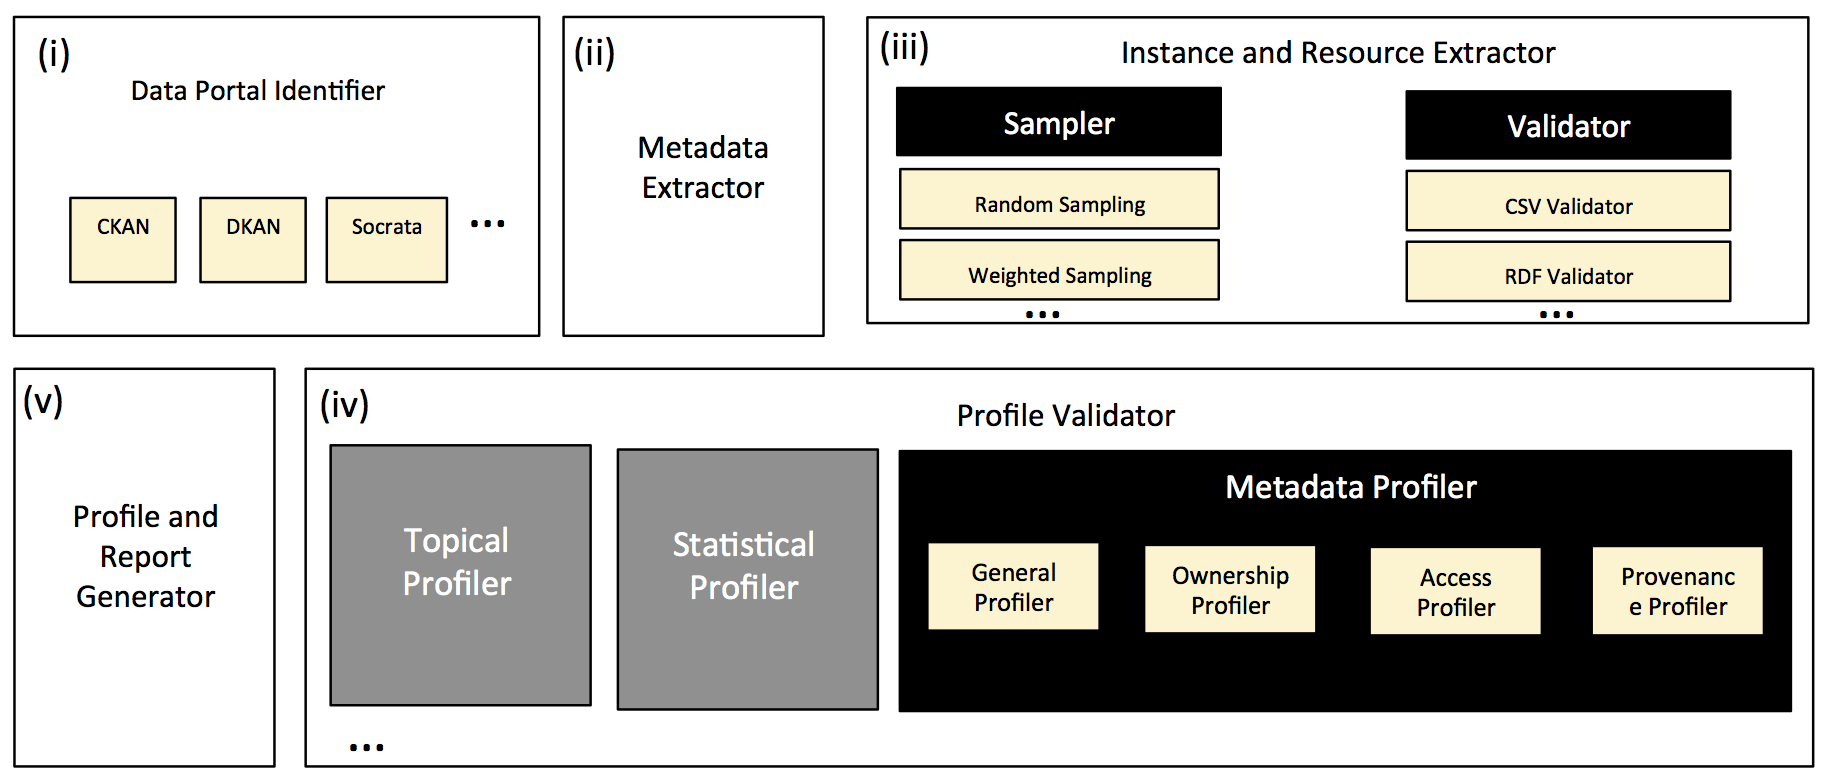
\includegraphics[scale=0.4]{figure-1_architecture.png}
  \caption{Processing pipeline for validating and generating dataset profiles}
  \label{fig:1}
\end{figure}

\subsection{Data Portal Identification}

Data portals can be considered as data access points providing tools to facilitate data publishing, sharing, searching and visualization. CKAN\footnote{http://ckan.org} is the world's leading open-source data portal platform powering websites like the DataHub, Europe's Public Data and the U.S Government's open data. Modeled on CKAN, DKAN\footnote{http://drupal.org/project/dkan} is a standalone Drupal distribution that is used in various public data portals as well. Socrata\footnote{http://www.socrata.com} helps public sector organizations improve data-driven decision making by providing a set of solutions including an open data portal. In addition to these tradition data portals, there is a set of tools that allow exposing data directly as RESTful APIs like Datatank\footnote{http://thedatatank.com} and Database-to-API\footnote{https://github.com/project-open-data/db-to-api}.

Identifying the software powering data portals is a vital first step to understand the API calls structure. Web scraping is a technique for extracting data from Web pages. We rely on several scraping techniques in the identification process which includes a combination of the following:

\begin{itemize}
  \item \textbf{URL inspection}: Check the existence of certain URL patterns. Various CKAN based portals are hosted on subdomains of the \texttt{http://ckan.net}. For example, CKAN Brazil (\texttt{http://br.ckan.net}).
  \item \textbf{Meta tags inspection}: The \texttt{<meta>} tag provides metadata about the HTML document. They are used to specify page description, keywords, author, etc. Inspecting the \texttt{content} attribute can indicate the type of the data portal. We use CSS selectors to check the existence of these meta tags. An example of a query selector is \texttt{meta[content*="ckan]} (all meta tags with the attribute content containing the string $CKAN$). This selector can identify CKAN portals whereas the \texttt{meta[content*="Drupal"]} can identify DKAN portals.
  \item \textbf{Document Object Model (DOM) inspection}: Similar to the meta tags inspection, we check the existence of certain DOM elements or properties. For example, CKAN powered portals will have DOM elements with class names like \texttt{ckan-icon} or \texttt{ckan-footer-logo}. A CSS selector like \texttt{.ckan-icon} will be able to check if a DOM element with the class name \texttt{ckan-icon} exists.\\
  The list of elements and properties to inspect is stored in a separate configurable object for each portal. This allows the addition and removal of elements as deemed necessary.
\end{itemize}

The identification process for each portal can be easily customized by overriding the default function. Moreover, adding or removing steps from the identification process can be easily configured.\\
After those preliminary checks, we query one of the portal's API endpoints. For example, DataHub is identified as CKAN, so we will query the API endpoint on \texttt{http://datahub.io/api/action/package\_list}. A successful request will list the names of the site's datasets, whereas a failing request will signal a possible failure of the identification process.

\subsection{Metadata Extraction}

Data portals expose a set of information about each dataset as metadata. The model used varies across portals. However, a standard model should contain information about the dataset's title, description, maintainer email, update and creation date, etc. We divided the metadata information into the following:

\textbf{General information}: General information about the dataset. e.g. title, description, ID, etc. This general information is manually filled by the dataset owner. In addition to that, tags and group information is required for classification and enhancing dataset discoverability. This information can be entered manually or inferred modules plugged into the topical profiler.

\textbf{Access information}: Information about accessing and using the dataset. This includes the dataset URL, license information i.e. license title and URL and information about the dataset's resources. Each resource has as well a set of attached metadata e.g. resource name, URL, format, size, etc.

\textbf{Ownership information}: Information about the ownership of the dataset. e.g. organization details, maintainer details, author, etc. The existence of this information is important to identify the authority on which the generated report and the newly corrected profile will be sent to.

\textbf{Provenance information}: Temporal and historical information on the dataset and its resources. For example, creation and update dates, version information, version, etc. Most of this information can be automatically filled and tracked.

Building a standard metadata model is not the scope of this paper, and since we focus on CKAN-based portals, we validate the extracted metadata against the CKAN standard model\footnote{http://demo.ckan.org/api/3/action/package\_show?id=adur\_district\_spending}.\\
After identifying the underlying portal software, we perform iterative queries to the API in order to fetch datasets metadata and persist them in a file-based cache system.
Depending on the portal software we can issue specific extraction jobs. For example, in CKAN based portals, we are able to crawl and extract the metadata of a specific dataset, all the datasets in a specific group e.g. LOD Cloud or all the datasets in the portal.

\subsection{Instance and Resource Extraction}

From the extracted metadata we are able to identify all the resources associated with that dataset. They can have various types like a SPARQL endpoint, API, file, visualization ,etc. However, before extracting the resource instance(s) we perform the following steps:

\begin{itemize}
  \item \textbf{Resource metadata validation and enrichment}: Check the resource attached metadata values. Similar to the dataset metadata, each resource should include information about its mimetype, name, description, format, valid de-referenceable URL, size, type and provenance. The validation process issue an HTTP request to the resource and automatically fills up various missing information when possible, like the mimetype and size by extracting them from the HTTP response header. However, missing fields like name and description that needs manual input are marked as missing and will appear in the generated summary report.
  \item \textbf{Format validation}: Validate specific resource formats against a linter or a validator. For example, node-csv\footnote{https://github.com/wdavidw/node-csv} for CSV files and n3\footnote{https://github.com/RubenVerborgh/N3.js} to validate N3 and Turtle RDF serializations.
\end{itemize}

Considering that certain dataset contains large amounts of resources and the limited computation power of some machines on which the framework might run on, a sampler module is introduced to execute various sample-based strategies detailed in \cite{scalableApproach} where they were found to generate accurate results even with comparably small sample size of 10\%.

\begin{itemize}
  \item \textbf{Random Sampling}: Randomly selects resources instances.
  \item \textbf{Weighted Sampling}: Weighs each resources as the ratio of the number of datatype properties used to define a resource over the maximum number of datatype properties over all the datasets resources.
  \item \textbf{Resource Centrality Sampling}: Weighs each resource as the ration of the number of resource types used to describe a particular resource divided by the total number of resource types in the dataset. This is specific and important to RDF datasets where important concepts tend to be more structured and linked to other concepts.
\end{itemize}

However, the sampler is not restricted only to these strategies. Strategies like those introduced in \cite{Leskovec:2006:SLG:1150402.1150479} can be configured and applied in the processing pipeline.

\subsection{Profile Validation}

A dataset profile should include descriptive information about the data examined. In our framework, we have identified three main profiling information. However, the extensibility of our framework allows for additional profiling techniques to be plugged in easily i.e. a quality profiling module reflecting the dataset quality. In this paper, we focus on the task of metadata profiling.\\

Metadata validation process identifies missing information and the ability to automatically correct them. Each set of metadata (general, access, ownership and provenance) is validated and corrected automatically when possible. Each profiler task has a set of metadata fields to check against. The validation process check if each field is defined and if the value assigned is valid.

There exist a bunch of special validation steps for various fields. For example, for ownership information where the maintainer email has to be defined, the validator checks if the email field is an actual valid email address. A similar process is done to URLs whenever found. However, we also issue an HTTP \texttt{HEAD} request in order to check if that URL is reachable or not. For the dataset resources, we use the \texttt{content-header} information when the request is successfull in order to extract, compare and correct further metadata values like mimetype and content size.

Despite the legal issues surrounding Linked Data licenses \cite{nomoneyLOD}, it is still considered a gold mine for organizations who are trying to leverage external data sources in order to produce more informed business decisions \cite{Boyd2011}. In \cite{mckinseyreport} the authors see the potential economic effect unfolding in education, transportation, consumer products, electricity, oil and gas, health care and consumer finance. They estimate the potential annual value enabled by Open Data in these domains to be 3 trillion US Dollars across seven domains. As a result, validating license related information is vital. However, from our experiments, we found out that datasets' license information is noisy. The license names if found are not standardized. For example, Creative Commons CCZero can be also CC0 or CCZero. Moreover,the license URI if found and if de-referenceable can point to different reference knowledge bases e.g. \texttt{http://opendefinition.org}. To overcome this issue, we have manually created a mapping file standardizing the set of possible license names and the reference knowledge base\footnote{https://github.com/ahmadassaf/opendata-checker/blob/master/util/licenseMappings.json}. In addition, we have also used the open source and knowledge license information\footnote{https://github.com/okfn/licenses} to normalize the license information and add extra metadata like the domain, maintainer and open data conformance.

\lstset{frame=single, caption={License mapping file sample}, label=json, captionpos=b}
\begin{lstlisting}[language=json]
{
  "license_id" : ["ODC-PDDL-1.0"],
  "disambiguations" : ["Open Data Commons Public Domain Dedication and License (PDDL)"]
},
{
  "license_id" : ["CC-BY-SA-4.0", "CC-BY-SA-3.0"],
  "disambiguations" : ["cc-by-sa", "CC BY-SA","Creative Commons Attribution Share-Alike"]
}
\end{lstlisting}


\textbf{Statistical profiling}\\

There exist a set of tools designed specifically to provide statistical information about a dataset (see section 2). Providing comprehensive statistical information about a dataset isn't in the scope of this paper. However, to show the extensibility of our framework we provide a simple RDF statistical profiler module that can be easily extended and configured. The information provided for each class is the number: triples, distinct objects, distinct literals, distinct IRI reference objects, distinct blank nodes objects, distinct subjects, distinct IRI reference subjects and distinct blank nodes subjects.\\

\textbf{Topical profiling}\\

Similar to the statistical profiler, a detailed survey of the existing tools can be found in the related work section. However, we implement a very basic topical profiler by applying Named Entity Disambiguation (NED) on the textual description and title of a dataset using DBpedia Spotlight \cite{Mendes:2011:DSS:2063518.2063519}.

\subsection{Profile and Report Generation}

The validation process highlights the missing information and presents them in a human readable report. The report can be automatically sent to the dataset maintainer email if exists in the metadata.

In addition to the generated report, the enhanced profiles are represented in JSON using the CKAN data model and are publicly available\footnote{https://github.com/ahmadassaf/opendata-checker/tree/master/results}.

Data portal administrators need an overall knowledge of the portal datasets and their properties. Our framework has the ability to generate numerous reports of all the datasets by passing formated queries. There are two main set of aggregation tasks that can be run:
\begin{itemize}
  \item \textbf{Aggregating meta-field values}: Passing a string that corresponds to a valid field in the metadata. The field can be flat like \texttt{license\_title} (aggregates all the license titles used in the portal or in a specific group) or nested like \texttt{resource>resource\_type} (aggregates all the resources types for all the datasets). Such reports are important to have an overview of the possible values used for each metadata field.
  \item \textbf{Aggregating key:object meta-field values}: Passing two meta-field values separated by a colon \texttt{:} e.g. \texttt{resources>resource\_type:resources>name}. These reports are important as you can aggregate the information needed when also having the set of values associated to it printed.
\end{itemize}

For example, the meta-field value query \texttt{resource>resource\_type} run against the LODCloud group will result in an array containing $[file,api,documentation ...]$ values. These are all the resource types used to describe all the datasets of the group. However, to be able to know also what are the datasets containing resources corresponding to each type, we issue a key:object meta-field query \texttt{resource>resource\_type:name}. The result will be a JSON object having the \texttt{resource\_type} as the key and an array of corresponding datasets titles that has a resource of that type.

\lstset{basicstyle=\scriptsize, backgroundcolor=\color{white}, breaklines=true, frame=single, caption={Excerpt of the DBpedia validation report}, label=report, captionpos=b}
\begin{lstlisting}
=======================================================================
                      Metadata Report
=======================================================================
group information is missing. Check organization information as they can be mixed sometimes
organization_image_url field exists but there is no value defined
=======================================================================
                      Tag Statistics
=======================================================================
There is a total of: 21 [undefined] vocabulary_id fields  100.00%
=======================================================================
                      License Report
=======================================================================
License information has been normalized !
=======================================================================
                      Resource Statistics
=======================================================================
There is a total of: 10 [missing] url-type fields  100.00%
There is a total of: 9 [missing] created fields  90.00%
There is a total of: 10 [undefined] cache_last_updated fields  100.00%
There is a total of: 10 [undefined] webstore_last_updated fields  100.00%
There is a total of: 10 [undefined] size fields  100.00%
There is a total of: 10 [undefined] hash fields  100.00%
There is a total of: 10 [undefined] mimetype_inner fields  100.00%
There is a total of: 7 [undefined] mimetype fields  70.00%
There is a total of: 10 [undefined] cache_url fields  100.00%
There is a total of: 6 [undefined] name fields  60.00%
There is a total of: 9 [undefined] webstore_url fields  90.00%
There is a total of: 9 [undefined] last_modified fields  90.00%
There is one [undefined] format field  10.00%
=======================================================================
                      Resource Connectivity Issues
=======================================================================
There are 2 connectivity issues with the following URLs:
   - http://dbpedia.org/void/Dataset
=======================================================================
                      Un-Reachable URLs Types
=======================================================================
There are: 1 unreachable URLs of type [file]
\end{lstlisting}

%%%%%%%%%%%%%%%%%%%%%%%%%%%%%%%%%%%%%%%
%%%  4. Experiments and Evaluation  %%%
%%%%%%%%%%%%%%%%%%%%%%%%%%%%%%%%%%%%%%%

\section{Experiments and Evaluation}
\label{sec:experiment}

In this section, we provide the experiments and evaluation of the proposed framework. All the experiments are reproducible by our tool and their results are available on the its Github repository.\\
We have run the framework on the LOD cloud containing 259 datasets at the time of writing this paper. We ran the instance and resource extractor in order to cache the metadata files for these datasets locally and ran the validation process which took around one and a half hour on a 2.6 Ghz Intel Core i7 processor with 16GB of DDR3 memory machine.\\
A CKAN dataset metadata describes three main sections in addition to the core dataset's properties. Those are the groups, tags and resources. Each section contains a set of metadata corresponding to one or more metadata type. For example, a dataset resource will have general information such as the resource name, access information such as the resource url and provenance information such as creation date. The framework generates a report aggregating all the problems in all these sections, fixing field values when possible. Errors can be the result of missing metadata fields, undefined field values or field value errors e.g. unreachable URL or incorrect email address.

Figures \ref{fig:2} and \ref{fig:3} show the percentage of errors found in metadata fields by section and by information type respectively. We found out that the most erroneous information for the dataset core information were ownership related as 41\% were missing or undefined. Datasets resources have the poorest metadata. 64\% of the general metadata, all the access information and 80\% of the provenance information contained missing or undefined values. Table \ref{tab:main} shows the top metadata fields errors in each metadata information type.

\begin{center}
\begin{tabular}{|c|c|c|c|c|c|}

\hline
\multicolumn{2}{|c|}{Metadata Field} & Error \% & Section & Error Type & Auto Fix\tabularnewline
\hline
\hline
\multirow{6}{*}{General } & group & 100\% & Dataset & Missing & -\tabularnewline
\cline{2-6}
 & vocabulary\_id & 100\% & Tag & Undefined & -\tabularnewline
\cline{2-6}
 & url-type & 96.82\% & Resource & Missing & -\tabularnewline
\cline{2-6}
 & mimetype\_inner & 95.88\% & Resource & Undefined & Yes\tabularnewline
\cline{2-6}
 & hash & 95.51\% & Resource & Undefined & Yes\tabularnewline
\cline{2-6}
 & size & 81.55\% & Resource & Undefined & Yes\tabularnewline
\hline
\multirow{5}{*}{Access } & cahce\_url & 96.9\% & Resource & Undefined & -\tabularnewline
\cline{2-6}
 & webstore\_url & 91.29\% & Resource & Undefined & -\tabularnewline
\cline{2-6}
 & license\_url & 54.44\% & Dataset & Missing & Yes\tabularnewline
\cline{2-6}
 & url & 30.89\% & Resource & Unreachable & -\tabularnewline
\cline{2-6}
 & license\_title & 16.6\% & Dataset & Undefined & Yes\tabularnewline
\hline
\multirow{5}{*}{Provenance } & cache\_last\_updated & 96.91\% & Resource & Undefined & Yes\tabularnewline
\cline{2-6}
 & webstore\_last\_updated & 95.88\% & Resource & Undefined & Yes\tabularnewline
\cline{2-6}
 & created & 86.8\% & Resource & Missing & Yes\tabularnewline
\cline{2-6}
 & last\_modified & 79.87\% & Resource & Undefined & Yes\tabularnewline
\cline{2-6}
 & version & 60.23\% & Dataset & Undefined & -\tabularnewline
\hline
\multirow{5}{*}{Ownership } & maintainer\_email & 55.21\% & Dataset & Undefined & -\tabularnewline
\cline{2-6}
 & maintainer & 51.35\% & Dataset & Undefined & -\tabularnewline
\cline{2-6}
 & author\_email & 15.06\% & Dataset & Undefined & -\tabularnewline
\cline{2-6}
 & organization\_image\_url & 10.81\% & Dataset & Undefined & -\tabularnewline
\cline{2-6}
 & author & 2.32\% & Dataset & Undefined & -\tabularnewline
\hline
\end{tabular}
\captionof{table}{Top metadata fields error \% by type} \label{tab:main}
\end{center}

\begin{figure}

\parbox{7cm}{\hspace*{-.2in}
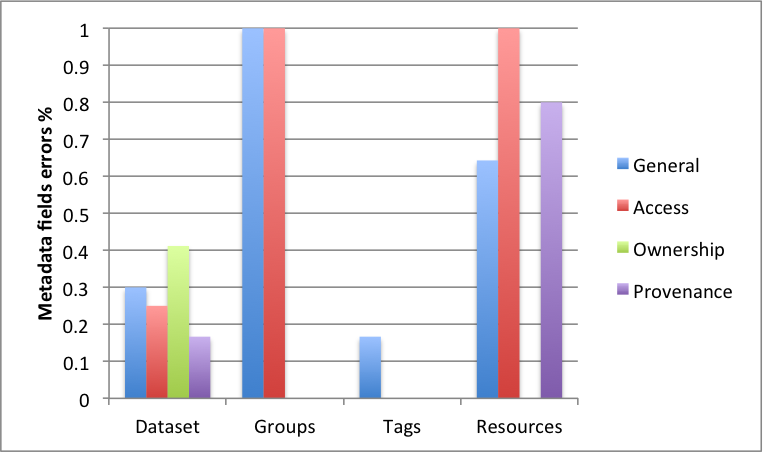
\includegraphics[width=.95\linewidth]{metadata_noise_by_section.png}
\captionsetup{textfont=small,singlelinecheck=off,justification=centering}
\caption{Error \% by section}
\label{fig:2}}
\qquad
\begin{minipage}{7cm}\hspace*{-.6in}
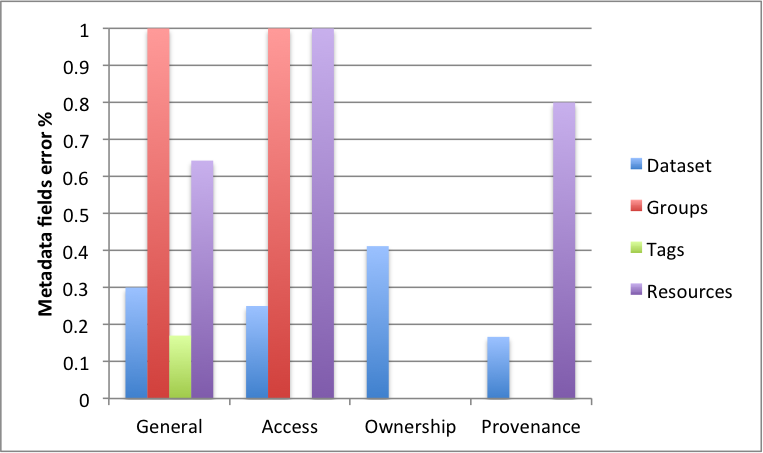
\includegraphics[width=.95\linewidth]{metadata_noise_by_metadata_type.png}
\captionsetup{textfont=small,singlelinecheck=off,justification=raggedright}
\caption{Error \% by information type}
\label{fig:3}
\end{minipage}

\end{figure}

We notice that 42.85\% of the top metadata problems can be fixed automatically. 44.44\% of these problems can be fixed by our tool while the others need tools that are plugged into the data portal. We further present and discuss the results grouped by metadata information type below.

\subsection{General information} 34 datasets (13.13\%) did not have valid \texttt{notes} values. \texttt{tags} information for the datasets were complete except for the \texttt{vocabulary\_id} as it was missing from all the datasets' metadata. All the datasets \texttt{groups} information were missing \texttt{display\_name, description, title, image\_display\_url, id, name}. After manual examination, we noticed a clear overlap between group and organization information. Many datasets like \texttt{event-media} used the organization field to show group related information (being in LOD Cloud) instead of the publishers details.\\

\subsection{Access information} 25\% of the datasets access information (being the dataset URL and any URL defined in its groups) has issues related to them (missing or unreachable URLs).
Three datasets (1.15\%) did not have a URL defined (tip, uniprot\-databases, uniprot\-citations) while 45 datasets (17.3\%) defined URLs were not accessible at the time writing this paper. One dataset did not have resources information (bio2rdf\-chebi) while the other datasets had a total of 1068 defined resources.\\
On the datasets resources level, we noticed wrong or inconsistent values in the \texttt{size} and \texttt{mimetype} fields. 20 (1.87\%) resources had incorrect \texttt{mimetype} defined, while 52 (4.82\%) had incorrect \texttt{size} values. These values have been automatically fixed based on the values defined in the HTTP response header. However, 44 datasets have valid \texttt{size} field values and 54 have valid \texttt{mimetype} field values where they were not reachable, thus providing incorrect information.\\
15 (68\%) fields of all the other access metadata are missing or have undefined values. Looking closely, we noticed that most of these problems can be easily fixed automatically by tools that can be plugged to the data portal. For example, the top six missing fields are the \texttt{cache\_last\_updated}, \texttt{cache\_url}, \texttt{url\-type}, \texttt{webstore\_last\_updated}, \texttt{mimetype\-\_inner} and \texttt{hash} which can be computed and filled automatically. However, the most important missing information which require manual entry are the dataset's \texttt{name} and \texttt{description} were missing from 817 (76.49\%) and 98 (9.17\%) resources respectively.
A total of 334 resources (31.27\%) URLs were not reachable, thus affecting highly the availability of these datasets. CKAN resources can be of various predefined types $(file, file.upload, api, visualization, code and documentation)$. The frameowork also breaks down these unreachable resources according to their types. 211 (63.17\%) resources did not have valid \texttt{resource\_type}, 112 (33.53\%) were files, 8 (2.39\%) and one (0.029\%) metadata, example and documentation types.

To have more details about the resources URL types, we created a $key:object meta-field values$ group level report on LOD cloud with \texttt{resources>format:title}. This will aggregate the resources format information for each dataset. We found out that only 161 (62.16\%) of the datasets valid URLs have SPARQL endpoints defined by \texttt{api/sparql} resource format. 92.27\% provided RDF example links and 56.3\% provided direct links to RDF down-loadable dumps.

The noisiest part of the access metadata was license information. A total of 43 datasets (16.6\%) did not have a defined \texttt{license\_title} and \texttt{license\_id} fields, where 141 (54.44\%) had missing \texttt{license\_url} field. However, we managed to normalize 123 (47.49\%) of the datasets' license information using the manual mapping file.

\subsection{Ownership information} Ownership information is divided into direct ownership (author and maintainer) and organization information. Four fields (66.66\%) of the direct ownership information were missing or undefined. The breakdown for the missing information is: 55.21\% \texttt{maintainer\_email}, 51.35\% \texttt{maintainer}, 15.06\% \texttt{author\_email}, 2.32\% \texttt{author}. Moreover, our framework performs checks to validate existing email values. 11 (0.05\%) and 6 (0.05\%) of the defined \texttt{author\_email} and \texttt{maintainer\_email} fields were not valid email addresses respectively.\\
For the organization information, two field values (16.6\%) were missing or undefined. 1.16\% of the \texttt{organization\_description} and 10.81\% of the \texttt{organization\-\_image\_url} information with two out of these URLs were unreachable.

\subsection{Provenance information} 80\% of the resources provenance information were missing or undefined. However, most of the provenance information e.g. \texttt{metadata\_created, metadata\_modified)} can be computed automatically by tools plugged into the data portal. The only field requiring manual entry is the \texttt{version} field which was found to be missing from 60.23\% of the datasets.

%%%%%%%%%%%%%%%%%%%%%%%%%%%%%%%%%%%%%%%
%%%  5. Conclusion and Future Work  %%%
%%%%%%%%%%%%%%%%%%%%%%%%%%%%%%%%%%%%%%%
\section{Conclusion and Future Work}
\label{sec:conclusion}

In this paper, we proposed a scalable automatic approach for extracting, validating, correcting and generating descriptive linked dataset profiles. This approach applies several techniques in order to check the validity of the metadata provided and to generate descriptive and statistical information for a particular dataset or for an entire data portal. Based on our experiments running the tool on the LOD cloud, we discovered that the general state of the datasets needs attention as most of them lack informative access information and their resources suffer low availability. These two metrics are of high importance for enterprises looking to integrate and use external linked data.\\
It has been noticed that the issues surrounding metadata quality affect directly dataset search as data portals rely on such information to power their search index. We noted the need for tools that are able to identify various issues in this metadata and correct them automatically. We found out that 32.25\% of all the metadata information can be automatically fixed, on which 50\%of them can be directly fixed by our framework. The rest are mainly provenance information that requires special treatment.\\
As part of our future work, we plan to introduce workflows that will be able to correct the rest of the metadata either automatically or through intuitive manually-driven interfaces. We also plan to integrate statistical and topical profilers to be able to generate full comprehensive profiles. We also intend to suggest a ranked standard metadata model that will help generate more accurate and scored metadata quality profiles. We also plan to run this tool on various CKAN based data portals, schedule periodic reports to monitor the evolvement of datasets metadata. Finally, at some stage, we plan to extend this tool for other data portal types like DKAN and Socrata.

\chapter{Hybrid Event Recommendation}    \label{ch:recommendation}
\graphicspath{{Part2/Chapter2/figures/}}

Recommendation in online services has gained momentum during the recent past years as a key factor to deliver personalized content. Reducing the information overload and assisting customers to make decision become part of primary concerns in the e-service area. To this aim, recommender systems attempt to provide efficient filters that decode the user interests, and optimize accordingly the information perceived. To help these systems predict items of interest, various clues are available ranging from a user profile, explicit ratings, to past activities and social interactions. For more details, Appendix~\ref{app:recommendation} describes two popular recommendation techniques, namely the content-based recommendation and the collaborative filtering.

Integrating a recommender system in event-based services is a key advantage to attract people attending events and to promote face-to-face social interactions. Indeed, the event recommendation can draw on different features such as the user preferences (ratings, likes, etc.), the attended events (visited places, involved artists), or even the social co-participation. Broadly speaking, the decision making upon attending events depends on some restrictions such as time, location, category, popularity and which friend will attend. However, the existing techniques (e.g. collaborative filtering and content-based methods) cannot cope at all with the complex inherent nature of such decision. In addition, a recommender system is often application-specific, that is, to be tuned according to the item context (e.g. type, reasons to select an item, etc.). Another challenge in our work is that events often involve different topics (e.g. different genres in one musical concert). As a result, the user profile constructed based on the attended events may contain a wide variety of topics. This leads to topically diverse profile that may conceal the effective user interests. 

To tackle these issues, we propose a hybrid recommender system based on Semantic Web technologies~\cite{Khrouf:RecSys2013}. Our belief is that a structured representation presents one solution to cope with the complexity of event-specific characteristics. This modeling will ensure a more straightforward way to explore and reason over the data. It makes possible to ask complex queries, for example, to retrieve events involving the same artist within a specific geographical area. In addition, the semantic model empowers the enrichment of event descriptions with additional information from Linked Data. Such enrichment can provide valuable inputs for the content-based recommender system~\cite{DiNoia:SEMANTICS12}.

In the second step of our approach, we propose to quantify the user interests based on topic modeling technique. The objective is to detect the user propensity towards specific topics. It will be integrated in the recommender system in order to control the impact caused by the diversity of a user profile. Finally, we exploit the collaborative participation assuming that the social information about ``which friend will attend an event'' plays an important role in decision making. In this work, we mainly investigate the extent to which the data enrichment, the social information and the user interests modeling can improve the system performance.


\section{Content-based Recommendation using Linked Data}
\label{sec:linkeddata-recommendation}
The principle of content-based (CB) recommendation is to suggest new items similar to those a user liked in the past. The similarity between items is computed based on the descriptive features of the item using a distance measure such as Cosine similarity, Pearson correlation and Latent Semantic Analysis~\cite{Landauer:1998}. The most common representation of the item is the keyword-based model, in which attributes are represented by weighted vectors of keywords usually computed by TF-IDF scheme (term frequency/inverse frequency). To build such a profile from unstructured data, feature extraction techniques are needed to shift the item description from the original representation to a structured form suitable for next processing (e.g. keyword vectors). This task becomes straightforward by the use of Semantic Web technologies. CB recommender systems can greatly benefit from the ease of ontology-enabled feature extraction, and the availability of Linked Data covering different domains to enrich the item profile. In the following, we explain how to compute the items similarity in Linked Data.

\subsection{Items Similarity in Linked Data}
In order to compute the similarity between items in Linked Data, we resolved to apply the approach proposed by Di Noia et al~\cite{DiNoia:SEMANTICS12}. The key idea is that semantically similar items from RDF graph are the subject of two RDF triples having the same property and the same object (where a triple=$<$subject,property,object$>$). The intuition behind is that: \textit{if two subjects are in the same relation to the same object, this is evidence that they may be similar subjects}. Technically, the approach is based on an adaptation of the classic Vector Space Model (VSM)~\cite{Salton:CACM75}, a well-known technique in Information Retrieval (IR). In this model, similarity between documents and queries is computed using their representative t-dimensional weighted vectors of discriminating terms. The application of VSM in RDF graph projects the Linked Data to 3-dimensional tensor where each slice represents an adjacency matrix corresponding to one property in the ontology. Indeed, the Linked Data network can be defined as a graph $G=(V,E)$ where $V$ is a set of resources and $E$ is the set of properties between resources in $V$. For each property $p$ in the set $E$, the related adjacency matrix presents the linkage between the subjects (on the rows) and the objects (on the columns) from $V$ via $p$. Then, a non null weight is assigned to each entry $X_{i,j,p}$ in the tensor for each existing triple $<i^{th}$ subject, $p^{th}$ property, $i^{th}$ object$>$. Figure~\ref{fig:tensor-slices} shows an example of tensor slices related to some properties, namely: \texttt{lode:atPlace}, \texttt{lode:involvedAgent} and \texttt{dc:subject}.

\begin{figure}
  \centering
  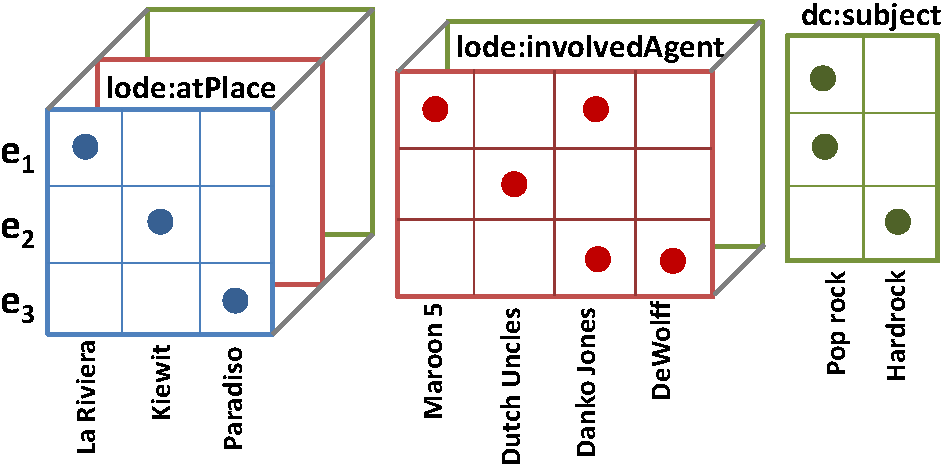
\includegraphics[scale=0.67]{tensor-slices.pdf}
  \caption{Tensor slices of some event properties (place, agent and subject)}
  \label{fig:tensor-slices}
\end{figure}

Assuming that the properties are semantically independent, we would be able to compute the similarity between events according to each property separately. The representation of an event $e_{i}$ according to the property $p$ is a t-dimensional vector indexing the terms/objects related to $e_{i}$ via $p$. The TF-IDF weight of each object $o$ is:

\begin{equation} \label{eq:weight}
w_{o,i,p}=f_{o,i,p} \ \cdot \ log \ \left(\frac {N}{m_{o,p}}\right)
\end{equation}
where $f_{o,i,p} = 1$ if a link exists between the node $e_{i}$ and the object $o$ via the property $p$, otherwise $f_{o,i,p}=0$. $N$ is the total number of events in the dataset, $m_{o,p}$ is the number of events linked to the object $o$ via the property $p$. Then, the similarity between two events $e_{i}$ and $e_{j}$ according to the property $p$ is computed using Cosine distance between their representative vectors as following:

\begin{equation}
sim^{p}(e_{i},e_{j})=\frac {\sum_{r=1}^{t} w_{r,i,p} \cdot w_{r,j,p}} {\sqrt{\sum_{r=1}^{t} w^{2}_{r,i,p}} \cdot \sqrt{\sum_{r=1}^{t} w^{2}_{r,j,p}}}
\end{equation}
This approach can be applied to detect similarity between subjects or objects of RDF triples. It has been successfully used to recommend movies and to improve the quality of content-based system~\cite{DiNoia:SEMANTICS12}. However, it is still limited when the adjacency matrix is very sparse such as the case of matrices associated with \texttt{lode:atPlace} and \texttt{lode:involvedAgent} properties. In fact, such predicates are characterized by the diversity of their object values, thus considered as discriminant properties. For instance, the t-dimensional vector related to \texttt{lode:atPlace} property has only one non-zero weight since an event is typically held at only one venue.


\subsection{Similarity-based Interpolation}

In order to mitigate the sparsity of the adjacency matrix, we propose to interpolate fictitious values based on the similarity between objects. Thus, we initially introduce a discriminability metric (i.e. discriminant power) to gain insight into the properties associated with highly sparse matrices. The metric is defined as following:

\begin{equation}
 Discriminability(p) = \frac{\mid{\{o\mid t=<s,p,o>\ \in G\}}\mid}{\mid{\ t=<s,p,o>\ \in G \mid}}
\end{equation}
where $G$ is the RDF graph, $t$ is the triple representing the link between the subject $s$ and the object $o$ via the property $p$. This formula quantifies the discriminability by the number of different object values on the target property. For instance, from a set of 1700 events (related to 10,323 agents, 627 places and 5,758 subjects), we found a discriminability score of 0.64 for the \texttt{lode:involvedAgent} and 0.45 for the \texttt{lode:atPlace}, while it is only equal to 0.10 for the \texttt{dc:subject} predicate. Furthermore, similar events are not necessary occurred at the same location or featuring the same performers. In order to reduce the discriminability impact, we interpolate fictitious weights in the adjacency matrix based on the similarity between objects as depicted in Figure~\ref{fig:interpolation}. 

\begin{figure}[htb]
  \centering
  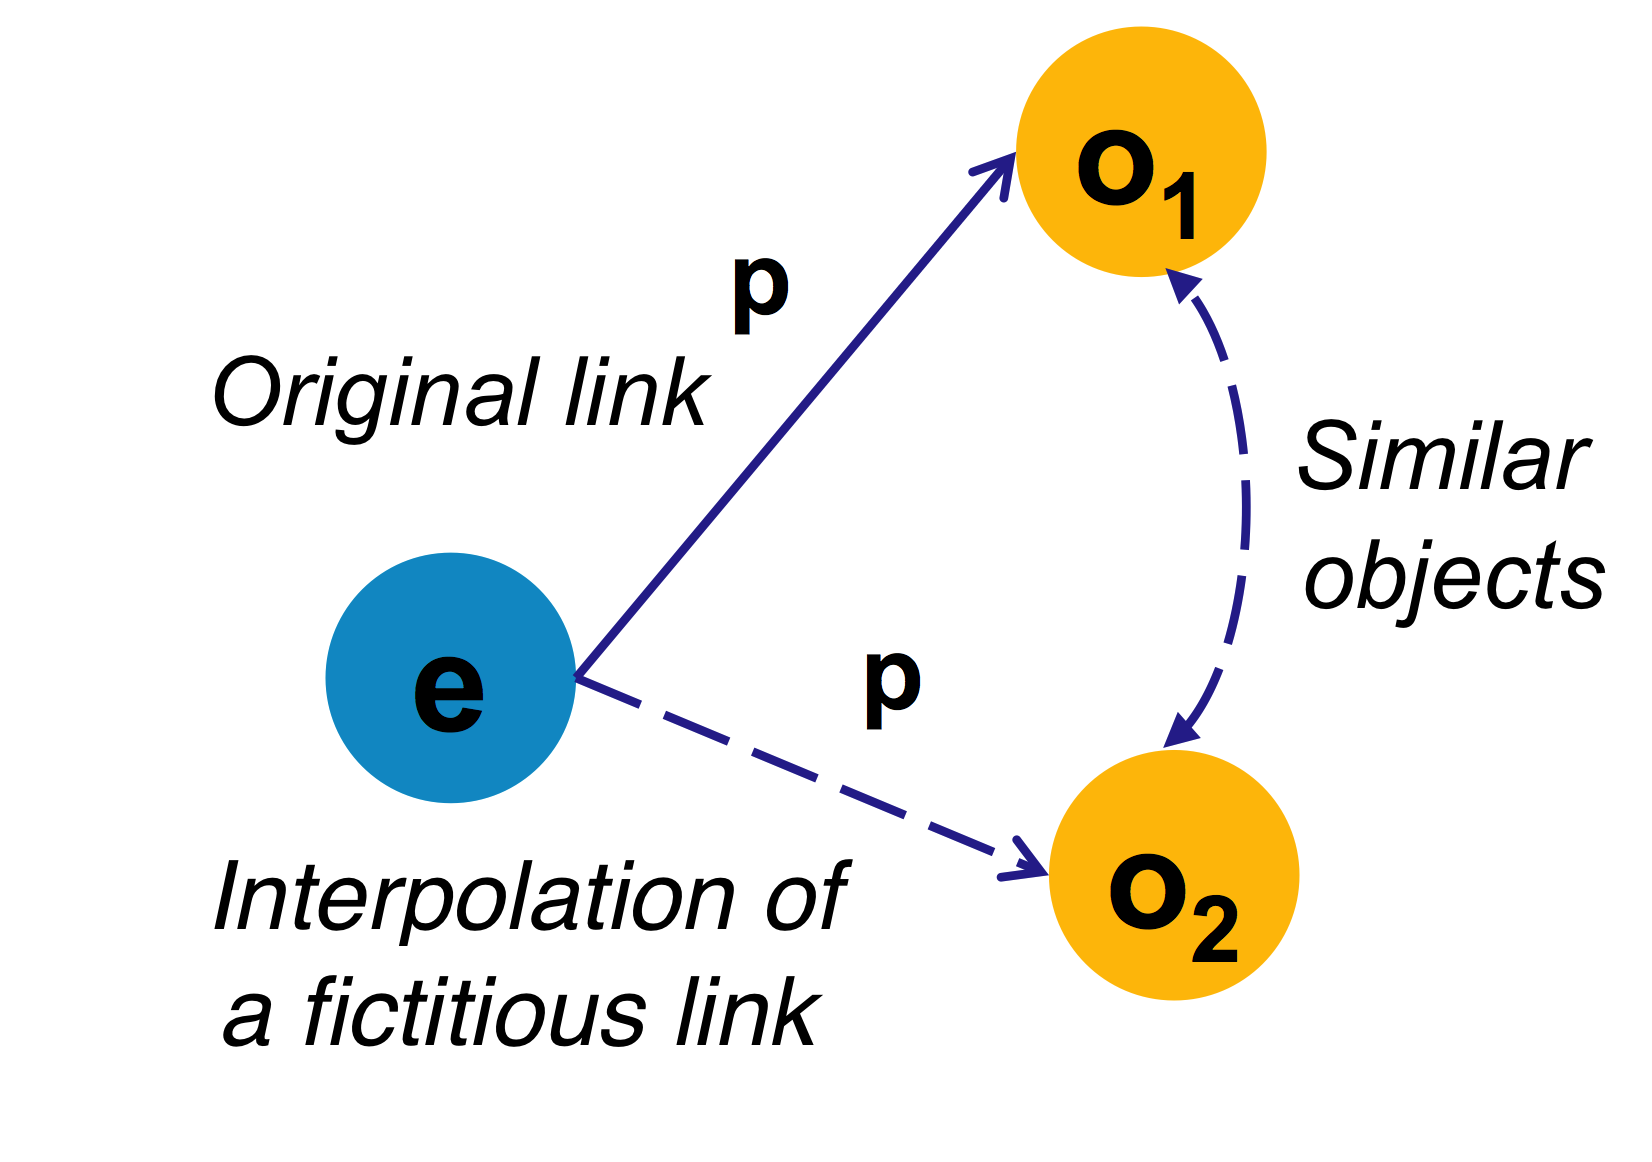
\includegraphics[scale=0.1]{sim-interpolation.png}
  \caption{Similarity-based Interpolation}
  \label{fig:interpolation}
\end{figure}

More precisely, if an object $o_{k}$ is similar to another object $o_{h}$, and if both $f_{o_{h},i,p} = 1$ and $f_{o_{k},i,p} = 0$, then $f_{o_{k},i,p} = sim(o_{k},o_{h})$. Note that $f_{o_{k},i,p}$ reflects the strength of the fictitious link which associates the event $e_{i}$ with the object $o_{k}$ via the property $p$. If the object $o_{k}$ is similar to more than one object originally linked to the event $e_{i}$, the weight $f_{o_{k},i,p}$ will be equal to the highest similarity score. Thus, for each object $o_{k}$, the equation~\ref{eq:weight} becomes:

\begin{equation}
w_{o_{k},i,p}= \max_{o_{h} \in H}sim(o_{k},o_{h}) \ \cdot \ log \ \left(\frac {N}{m_{o_{k},p}}\right)
\end{equation}
where $H$ is the set of objects originally linked to the event $e_{i}$. The intuition behind this formula is that: \textit{if two subjects are in same relations to similar objects, this is evidence that they may be similar subjects}. We do not pay attention to how similarity between objects is computed. In fact, this measure depends on the nature of the object itself and there exist several existing techniques that can be used. In our case, we exploit the similarity scores between agents (i.e. artists) provided by third party services such as Last.fm, and we compute the normalized geographical distance between venues.


%%%%%%%%%%%%%%%%%%%%%%%%%%
%%%  3. Event Recommendation %%%
%%%%%%%%%%%%%%%%%%%%%%%%%%

\section{Event Recommendation }
\label{sec:event-recommendation}
Different from a classic item, events occur at a specific place and during a period of time to become worthless for recommendation. Moreover, while a classic item (e.g. movie, book) continuously receives useful feedback, an event has few rating due to its transiency. In our dataset, these ratings are represented by the binary user-event attendance matrix which has a sparsity rate equal to 98\% (i.e. a set of users attend a very limited number of events). As a solution, one can address event recommendation using CB recommender system that exploits the matching of event attributes with the user profile. This perfectly complies with the constraints considered when it comes to decide whether or not to attend an event. Metadata such as distance, time, topics and artists are important and influential factors in such decision. Still, the CB recommendation might suggest items with a limited diversity and overlook the social information regarding the question ``which friend is going?''. To reduce this gap, we propose to enhance its performance by enriching the content using Linked Data, and by improving the detection of the user interests. Then, we incorporate the social information using Collaborative Filtering (CF) method, thus producing a hybrid recommendation.

%%%%%%%%%%%%%%%%%%%%%%%%%%%%%%%%%%%%%%%%%
%%%  3.1 Content-based Recommendation %%%
%%%%%%%%%%%%%%%%%%%%%%%%%%%%%%%%%%%%%%%%%

\subsection{Content-based Recommendation}
The CB recommender system suggests future events similar to those a user has attended in the past. We assume that there is a sufficient number of past attended events in the user profile to avoid the \textit{cold-start} problem\footnote{The problem to produce good recommendations for new users where nothing is known about their preferences}, which is out of the scope of the present work. In order to predict the participation of the user $u$ to the event $e_{i}$, we combine the similarity values between events as following: 

\begin{equation}\label{eq:rankcb}
rank_{cb}(u,e_{i})= \frac{\sum_{e_{j} \in E_{u}} \sum_{p\in P} \ \alpha_{p}\ sim^p(e_{i},e_{j})}{\mid P \mid\  \cdot \mid E_{u}\mid}
\end{equation}
where $E_{u}$ is the set of past events attended by the user $u$, $P$ is the set of properties shared between two events $e_{i}$ and $e_{j}$, and $\alpha_{p}$ is the weight that reflects the contribution of the property $p$ in the recommendation.

The properties selected to compute the similarity between events are those which are related to the location, subjects (tags) and involved agents (artists). In contrast, the temporal information is not considered in this work and left for future study. Our belief is that temporality could be harnessed to index the recent events in the user profile, thus reducing the computation. Still, there is a need to deeply investigate the impact that the reduction of the user profile has on the system performance. 

\myparagraph{Geographic Closeness}
In recent research study, it has been shown that users generally tend to attend nearby entertainment events~\cite{Quercia:ICDM10}. This fact makes the location a valuable feature in event recommendation. In our approach, we need to measure the similarity between events according to the \texttt{lode:atPlace} property. Thus, we normalize the distance between two locations using a specific threshold $\theta$ which needs to be determined. As the user home is missing in our data, we measure the distance between attended events for each user as depicted in Figure~\ref{fig:attendance-distance}. Note that the attendance rate becomes extremely low from $\theta=80$ Km. We consider that this value is the normalization threshold from which the similarity between events is equal to zero according to the \texttt{lode:atPlace} property.

\begin{figure}[H]
  \centering
  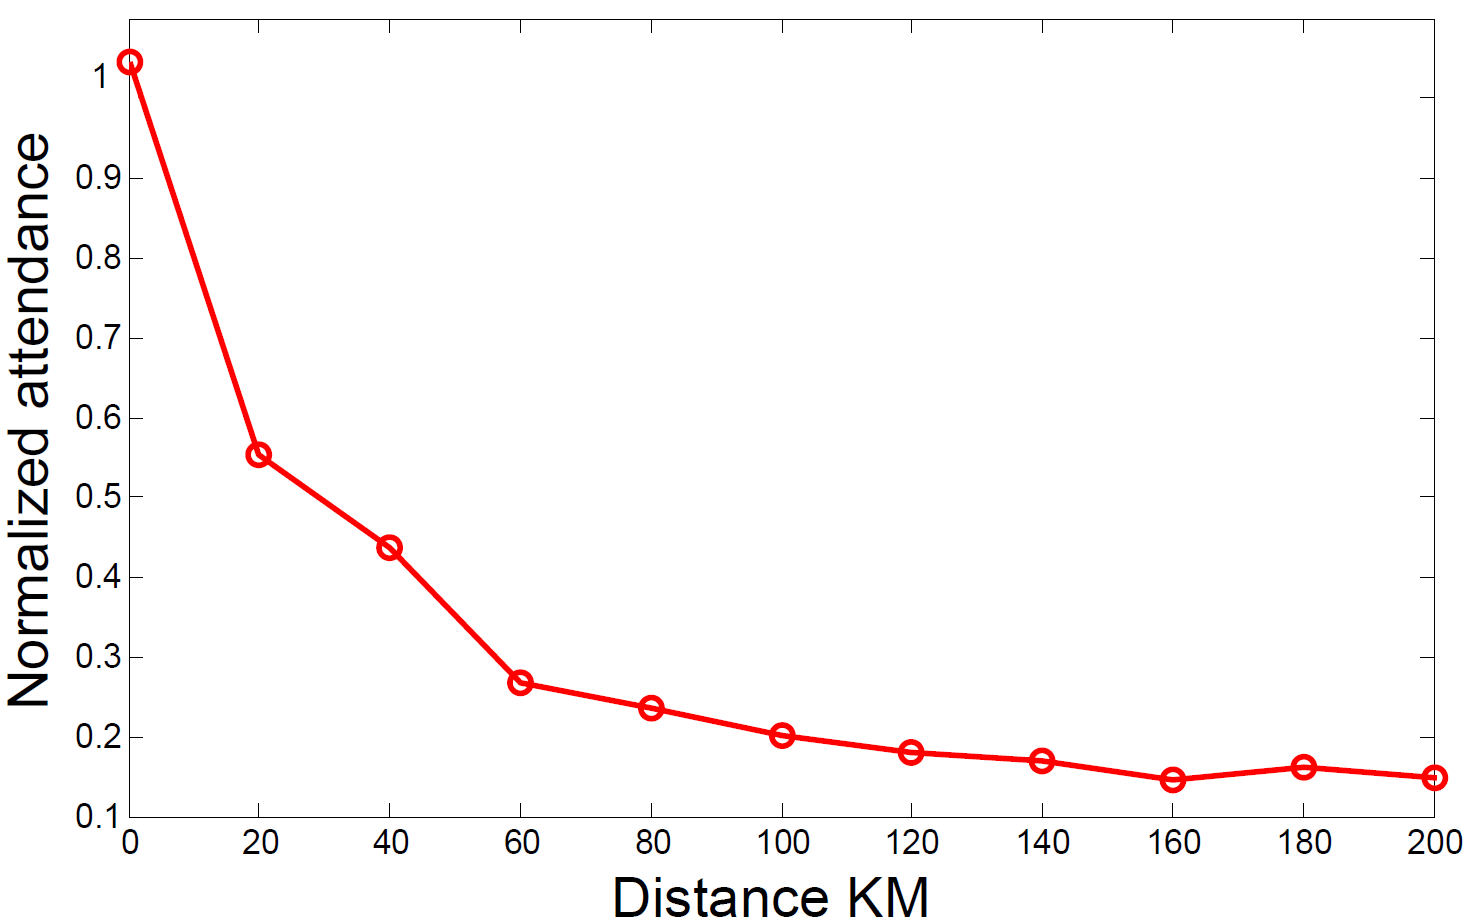
\includegraphics[scale=0.22]{attendance-distance.png}
  \caption{Normalized average attendance per distance}
  \label{fig:attendance-distance}
\end{figure}

\myparagraph{Enrichment with Linked Data} One method to enrich the item profile from Linked Data is to consume background information from DBpedia. The key advantage of DBpedia is the availability of semantically rich data in various domains. Using the mapping between EventMedia and DBpedia, we enrich the topics of an event using the DBpedia topics (e.g. genres) related to the involved artists. More precisely, we retrieve the categories associated with the property \texttt{dcterms:subject} of artists by simply querying the DBpedia SPARQL endpoint\footnote{\url{http://dbpedia.org/sparql}}. The reason behind our interest in DBpedia is that topics are accurately labeled and classified.

\subsection{User Interests Modeling}
One fundamental goal in the recommender system is to suggest new items that best fit the user interests. In our case, this is particularly difficult to achieve due to the presence of topically diverse events. In fact, the real-world social events can be classified into large set of categories ranging from large festivals and conferences to small concerts and social gatherings. When attending an event, the user might be interested in a specific show or artist or might have broad interests. In consequence, relying on event similarity according to the \texttt{dc:subject} property can be influenced by the topical diversity of tags related to events in the user profile. To alleviate this impact, we leverage the Latent Dirichlet Allocation (LDA)~\cite{Blei:MLR03} for detecting the relevant user interests as previously described in Section~\ref{sec:user-interest}.

\begin{figure}[htb]
  \centering
  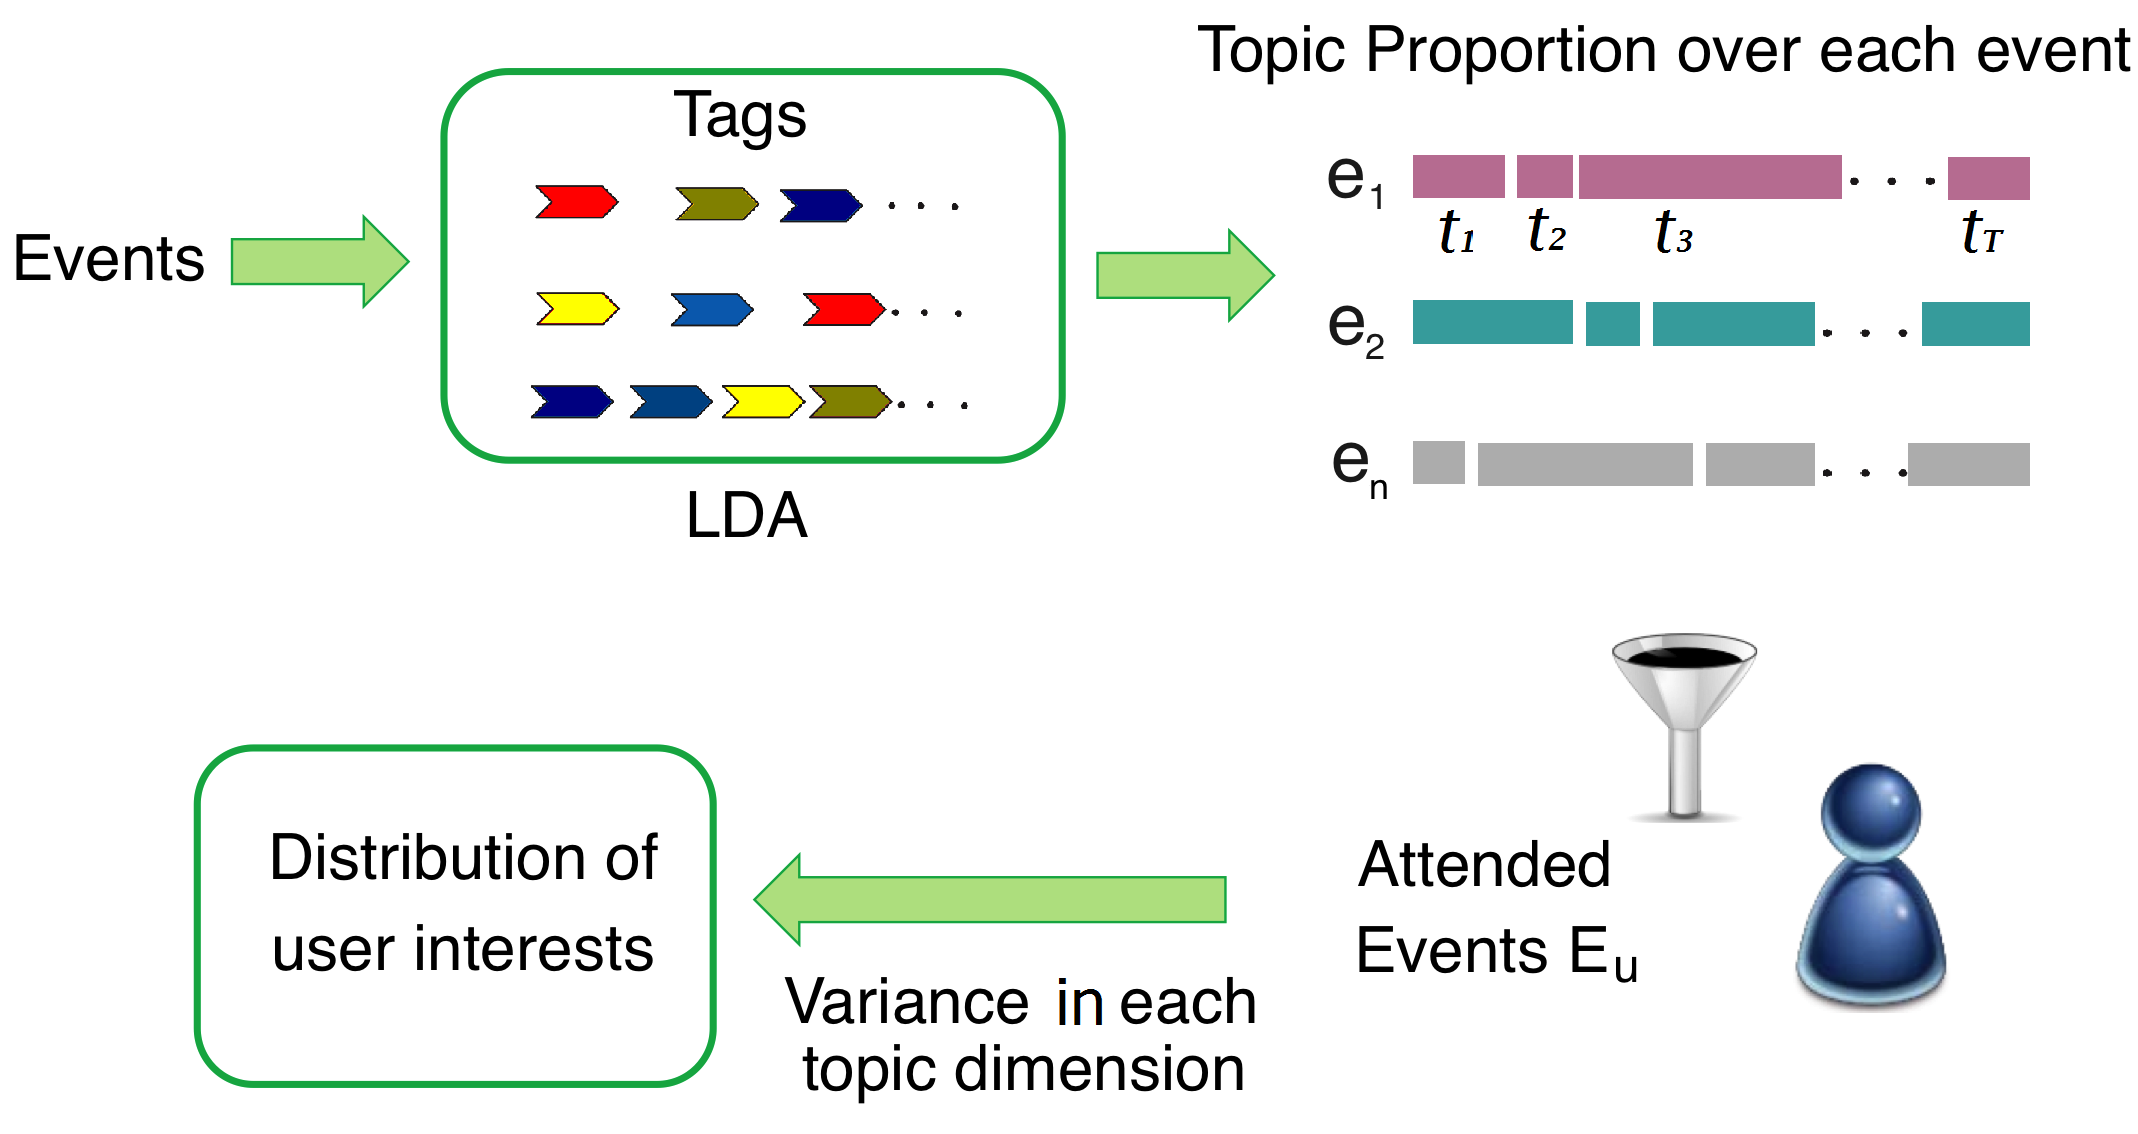
\includegraphics[scale=0.2]{user-div.png}
  \caption{The pipeline of user Interests modeling}
  \label{fig:div-approach}
\end{figure}

Figure~\ref{fig:div-approach} illustrates the pipeline of the user interests modeling. For each event $e_{i}$ having a set of tags, LDA generates a $T$-dimensional vector of topic proportions $\Theta_{i} = [\theta^{1}_{i},\theta^{2}_{i},...\theta^{T}_{i}]$, where $T$ is the number of topics and $\Theta_{i}$ reflects the semantic categories of the event. Then, we compute the variance in each topic dimension $t$ over all the events $E$ attended by a user $\Theta^{t} = [\theta^{t}_{1},\theta^{t}_{2},...\theta^{t}_{E}]$. The diversity score of each corresponding user is the mean of the variances of all the topics dimensions (mean of $\Theta^{1},\Theta^{2}...\Theta^{T})$. 

This approach as introduced by Wu et al.~\cite{Hao:AHJ12} has been originally designed to study the diverseness of individual tastes. But, we think that it is also helpful to detect user's propensity from a topically diverse profile. Indeed, events can be divided into two classes: those related to very few topics or those related to many topics. We consider that events in the first class are those which really exhibit the user interests. Using the variance, we are able to detect high proportions within topic dimension given that this dimension is likely to also contain low proportions (i.e. events are not regularly distributed over the topics).

As an example, Figure~\ref{fig:diversity-scores} shows the normalized diversity scores obtained from a sample of 1,000 Last.fm users. In Figure~\ref{fig:diversity_a}, it is shown that most of diversity scores range from $0.3$ to $0.5$ indicating that users have relatively high interests in specific topics. The diversity scores near to 1 represent users having strong interests in very few topics such as the case of the user plotted in Figure~\ref{fig:diversity_b}. This user has a strong bias specifically towards the topic $9$. Finally, the diversity scores close to zero generally represent the users associated with few attended events (i.e. the cold-start problem).

\begin{figure}[htb]
\centering
\subfigure[]{\label{fig:diversity_a}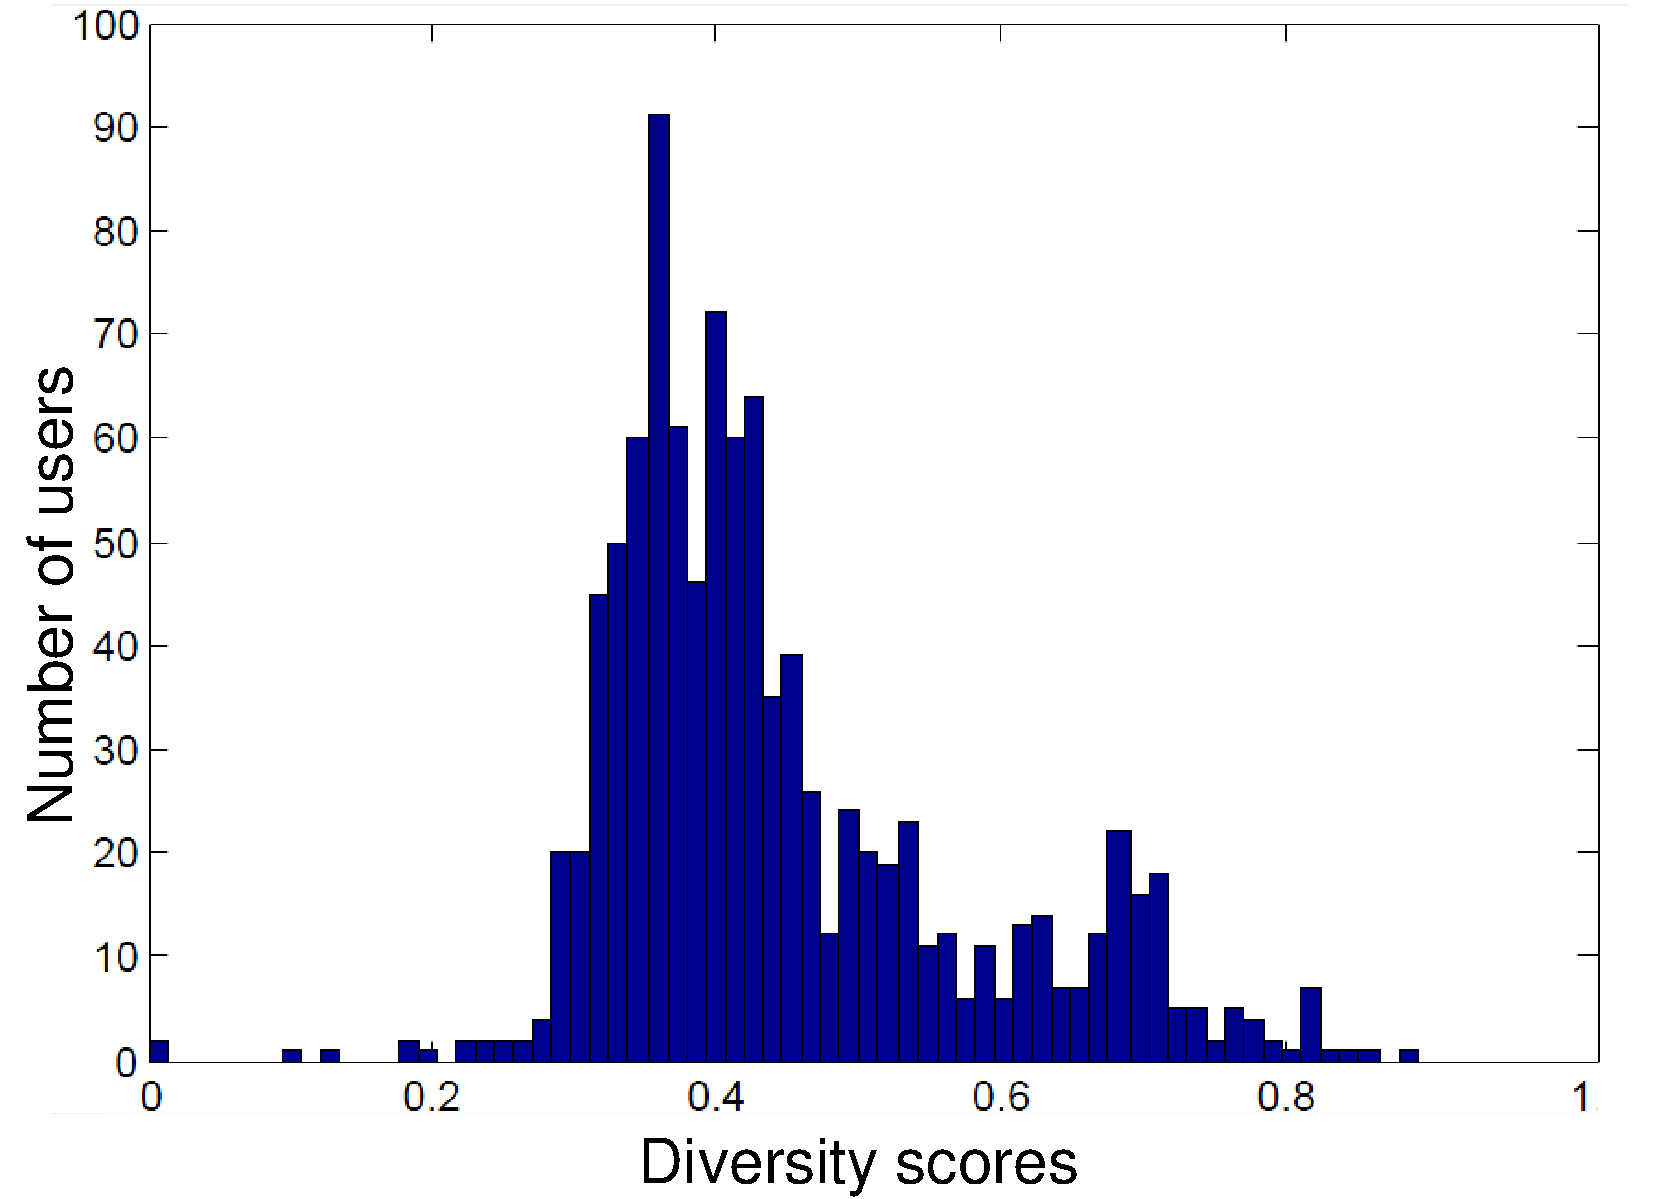
\includegraphics[height=50mm,width=.48\linewidth]{users-diversity.pdf}}
\subfigure[]{\label{fig:diversity_b}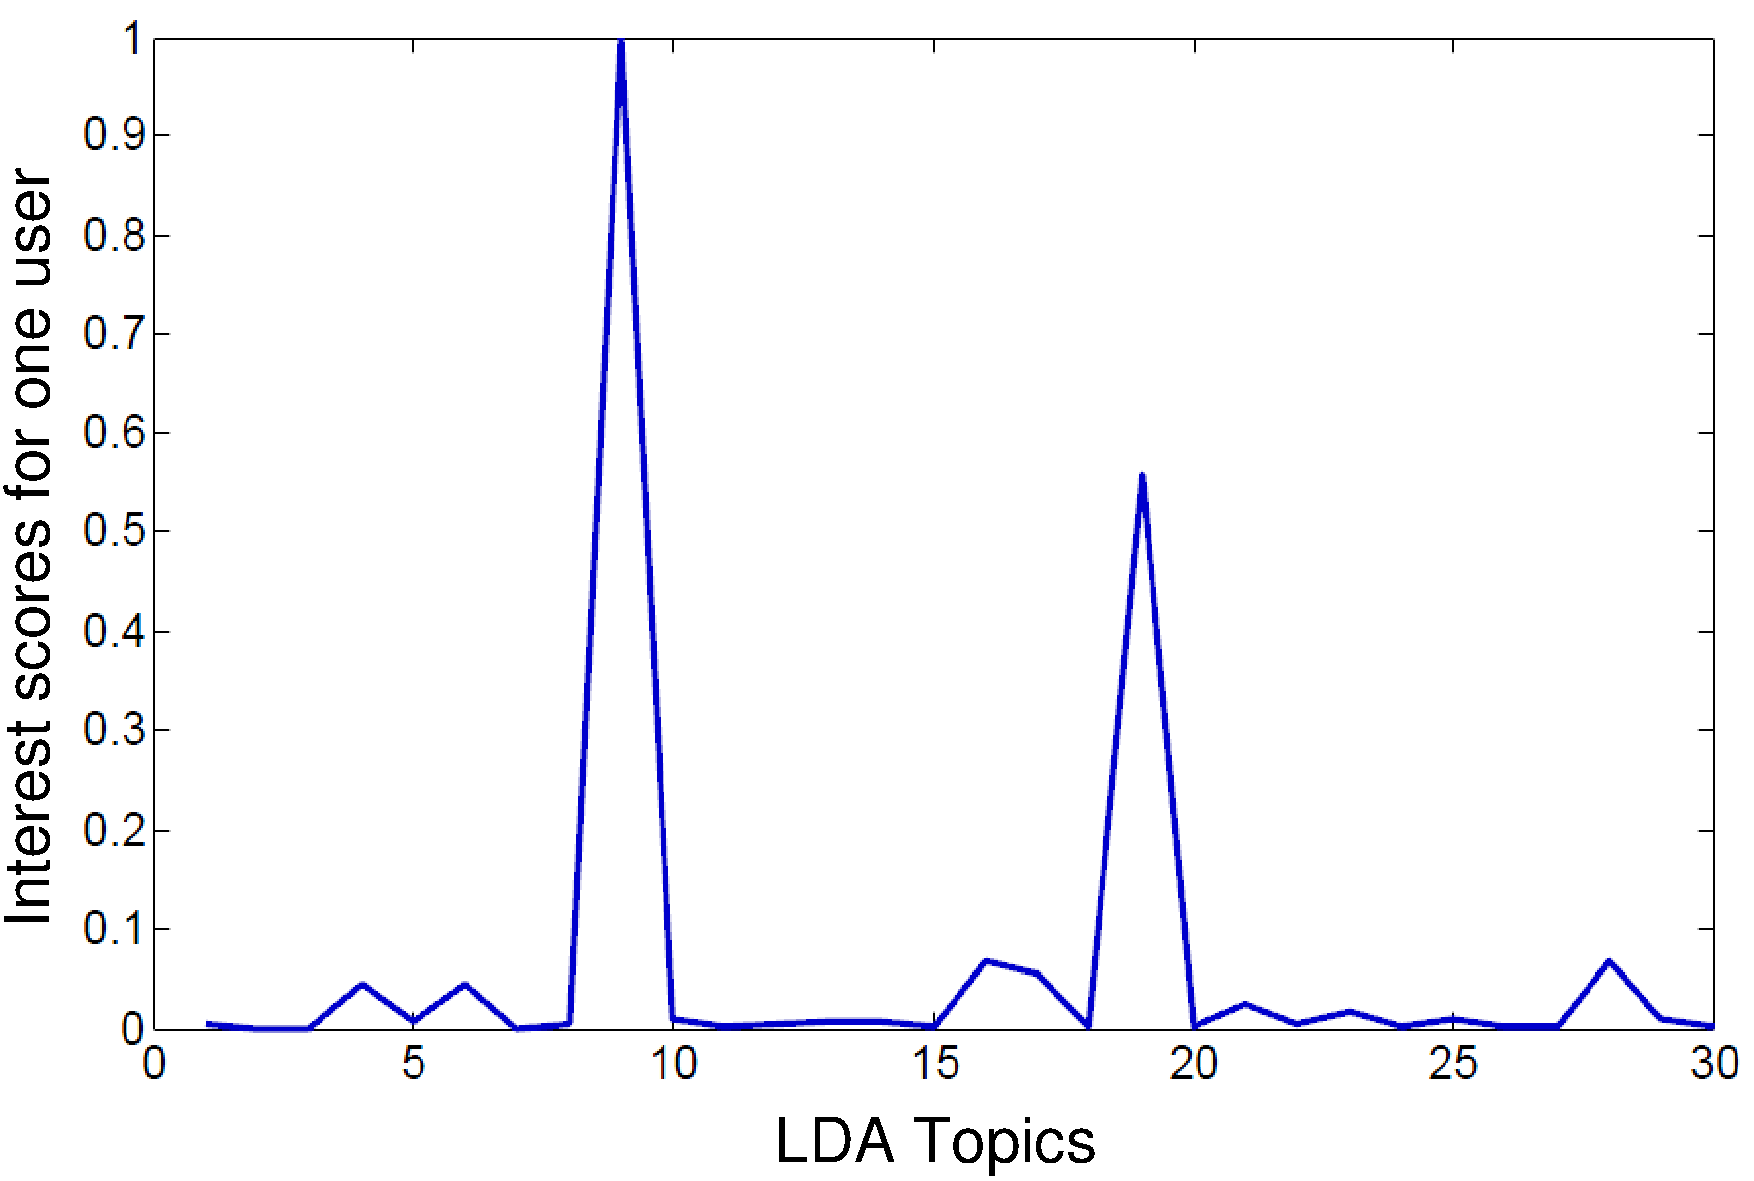
\includegraphics[height=50mm,width=.48\linewidth]{one-user-diversity.pdf}}
\caption{Distribution of topical diversity scores with T = 30: (a) for all the users; (b) for one specific user.}
\label{fig:diversity-scores}
\end{figure}

To take into account the effective user interests in a recommender system, we give emphasis to the events which are more likely to correspond to the user interests. We assign different weights $\beta$ to the events included in the peaks of interest, and to those which are out of these peaks. These weights are then estimated using training methods. The content-based recommendation is extended as following:

\begin{equation}\label{eq:rankcb++}
rank_{cb++}(u,e_{i})= \frac{\sum_{e_{j} \in E_{u}} \sum_{p\in P} \ \alpha_{p}\ \beta_{p} \  sim^p(e_{i},e_{j})}{\mid P \mid\  \cdot \mid E_{u}\mid}
\end{equation}
where $\beta_{p} = 1$ if the property $p$ is different from \texttt{dc:subject}, otherwise the $\beta_{subject}$ is an estimated value depending on whether the event $e_{j}$ corresponds to the user interests or not.


%%%%%%%%%%%%%%%%%%%%%%%%%%%%%%%%%%%%
%%%  3.3 Collaborative filtering %%%
%%%%%%%%%%%%%%%%%%%%%%%%%%%%%%%%%%%%

\subsection{Collaborative Filtering}
A form of social interactions is the collaborative participation such as co-authoring a paper or co-attending an event. In~\cite{Liu:KDD12}, Liu et al. highlight the existence of an offline social network built from the co-attendance of social events. Accordingly, we consider that two users involved in the same event can potentially have a stronger tie than other users. Our assumption is that the more events in which users involve, the stronger is their tie. Thus, the co-attendance can be a clue to provide information at first glance about which ``friends'' will attend an event. Moreover, our dataset contains the users' RSVP that express their intent to join social events, which can be exploited to predict unknown intents. However, unlike the traditional user-based collaborative filtering (CF), we decide to not only consider the similarity between users, but also the contribution of a group of friends. We define the following formula as the prediction that a user $u_{i}$ will attend an event $e$ based on the RSVP of his/her co-attendees (i.e. users who have attended past events with the user $u_{i}$):


\begin{equation}\label{eq:rankcf}
rank_{cf}(u_{i},e)= \frac{\sum_{j \in C } \ a_{i,j}}{\mid C \mid } \ \cdot \  \frac{\mid E_{i} \cap ( \cup_{j \in C } E_{j}) \mid}{\mid E_{i} \mid}
\end{equation}
where $C$ is the set of co-attendees who will attend the event $e$, $E_{i}$ is the set of attended events by the user $u_{i}$, and $a_{i,j}$ is the fraction of common events between the users $u_{i}$ and $u_{j}$ by the cardinality of $E_{j}$. Note that the weight $a_{i,j}$ reflects whether the most of events which are attended by the user $u_{j}$ are also attended by the user $u_{i}$. The rationale behind this formula is two-fold: (1) in the first part, we consider the contribution of each co-attendee individually; (2) in the second part, we consider the co-attendees as a group of friends, and we assume that the more events they attended together with the user $u_{i}$, the more strongly is their relationship.

%%%%%%%%%%%%%%%%%%%%%%%%%%%%%%%%%%
%%%  3.4 Hybrid Recommendation %%%
%%%%%%%%%%%%%%%%%%%%%%%%%%%%%%%%%%

\subsection{Hybrid Recommendation}
To combine the predictions of both CB and CF recommender systems, we propose a weighted hybridization using a linear combination of predicted rank. Taking into account the user diversity and combining the equations (\ref{eq:rankcb++}) and (\ref{eq:rankcf}), we proposed the following function:

\begin{equation}\label{eq:hybrid}
rank(u,e)= rank_{cb++}(u,e) + \ \alpha_{cf}\ rank_{cf}(u,e)
\end{equation}
where $\alpha_{cf}$ is the weight of CF method estimated in conjunction with the weights of CB features using optimization functions for training the system.


%%%%%%%%%%%%%%%%%%%%%%
%%%  5. Evaluation %%%
%%%%%%%%%%%%%%%%%%%%%%

\section{Evaluation}
\label{sec:evaluation}
In this section, we carry out a set of experiments measuring the precision and recall metrics to assess the contribution of each step in our approach, and to evaluate the performance of our system compared with existing approaches.

%%%%%%%%%%%%%%%%%%%%%%%%%%%%%%%
%%%  5.1 Real World Dataset %%%
%%%%%%%%%%%%%%%%%%%%%%%%%%%%%%%

\subsection{Real-world Dataset}
We use the EventMedia dataset and particularly the Last.fm directory which contains a large number of active users. Using SPARQL, we collected 2,436 events, 481 active users whose the attendance rates are within [15,50], generating 12,729 distinct consumption (i.e. user-event pairs). This set of events are related to 14,748 distinct artists, 897 locations and 4265 tags (music domain). For the evaluation, we use a test set containing the most recent 30\% of the consumption and a training test with the remaining 70\% consumption. Then, we measure two metrics used in top-N recommendation task: Precision is the ratio of correctly recommended items and the length of the recommendation $N$; Recall is the ratio of correctly recommended items and the total number of future consumption. Precision and Recall are computed at different $N$ values.

%%%%%%%%%%%%%%%%%%%%%%%%%%%%%%%%%
%%%  4. Learning Rank Weights %%%
%%%%%%%%%%%%%%%%%%%%%%%%%%%%%%%%%

\subsection{Learning Rank Weights}
\label{sec:learning}
To learn the weights of our prediction function, we first test the linear regression with gradient descent that minimizes the least-squares cost function. Then, we use two evolutionary computation methods, namely the Genetic Algorithm (GA) and the Particle Swarm Optimization (PSO) motivated by their success in a wide range of tasks (details in Appendix~\ref{app:optimization}).

%%% Genetic Algorithm %%%

To apply GA in our approach, a chromosome is represented by a vector of the coefficients that need to be estimated. Each chromosome is then evaluated using a fitness function. This function aims to minimize the prediction error and thus maximize the precision of results. Table~\ref{tab:ga-param} shows the GA setting parameters.

\begin{table}[H]
\centering{
\begin{tabular*}{11cm}{c @{\extracolsep{\fill}} ccc}
\hline
Population size & Iterations & crossover & mutation  \\
\hline
30 & 80 & 0.9 & 0.01  \\
\hline
\end{tabular*}
\caption{Setting of GA parameters for event recommendation}
\label{tab:ga-param}
}
\end{table}


%%% Particle Swarm Optimization %%%

As for PSO, a particle is represented by a vector of weights and the fitness function aims at maximizing the precision. Table~\ref{tab:pso-param-2} shows the PSO setting parameters.

\begin{table}[H]
\centering{
\begin{tabular*}{11cm}{c @{\extracolsep{\fill}} cccc}
\hline
Population size & Iterations & $c_{1}$ &  $c_{2}$ & inertia   \\
\hline
30 & 80 & 1.494 & 1.494 & 0.729\\
\hline
\end{tabular*}
\caption{Setting of PSO parameters for event recommendation}
\label{tab:pso-param-2}
}
\end{table}


\subsection{Experiments}
First, we show in Table~\ref{tab:sparsity-tab} the sparsity rates of similarity matrices according to each property. We can see the efficiency of our method to discover latent similarity between events especially for discriminant properties. This highlight the importance of the similarity-based interpolation and the enrichment using Linked Data. Unlike the keyword-based recommender systems, the interpolation is straightforward in our system thanks to the ontology-based data representation.

\begin{table}[H]
\centering{
\begin{tabular*}{8cm}{c @{\extracolsep{\fill}} ccccc}
\hline
Task & location & agent & subject \\
\hline
   (1) & 0.9942 & 0.9174 & 0.3175 \\
\hline
   (2) & 0.6854 & 0.7392 & 0.2843 \\
\hline
\end{tabular*}
\caption{Sparsity rates of the similarity matrices before (1) and after (2) the similarity-based interpolation (for location and agent) and data enrichment with DBpedia (for subject)}
\label{tab:sparsity-tab}
}
\end{table}

Second, we assess the performance of the training methods to learn the coefficients $\alpha$ in the hybrid recommendation algorithm. Note that for this experiment, we do not include the user interests model and we set the $\beta_{subject}$ equal to 1. This experiment aims to rather compare the performance of optimization methods. 

\begin{figure}[htb]
  \centering
  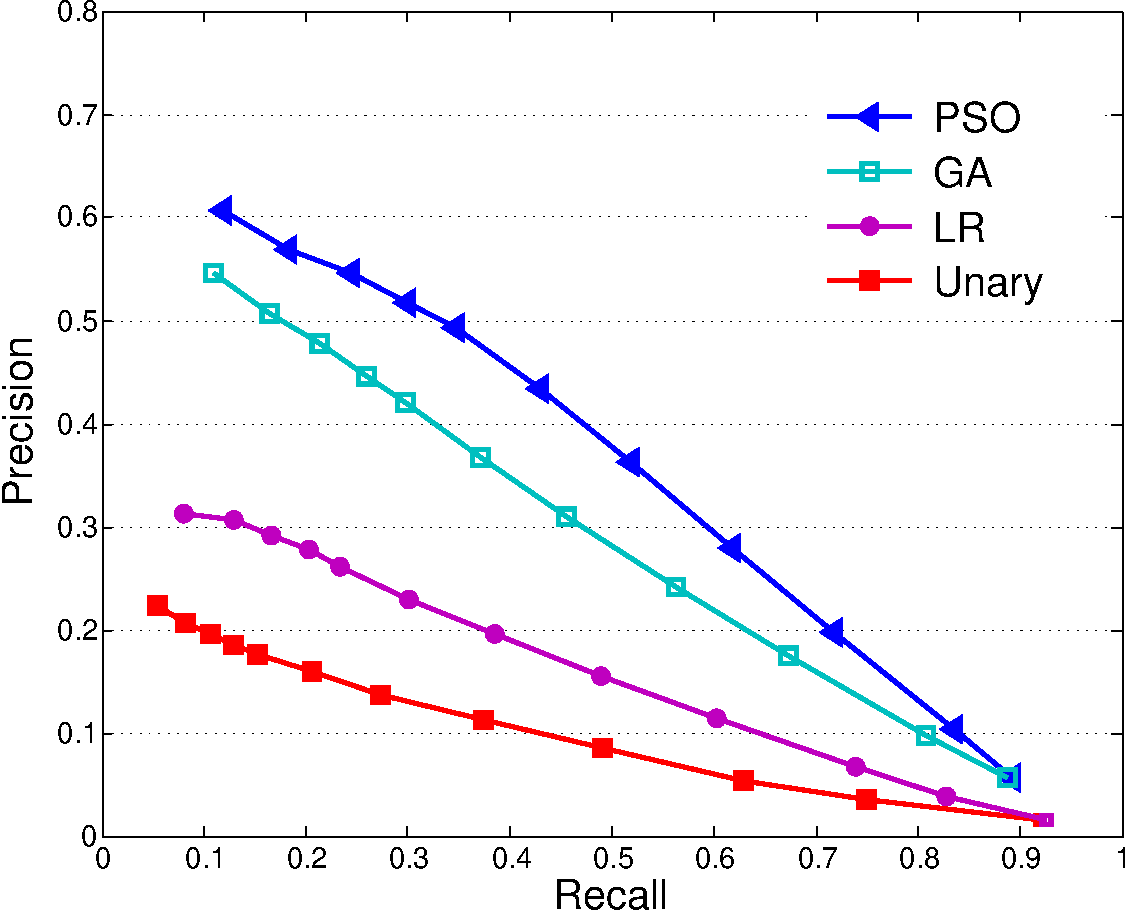
\includegraphics[height=62mm,width=80mm]{training-comparison.pdf}
  \caption{Recall and Precision using different approaches to estimate the vector $\alpha$}
  \label{fig:training-comparison}
\end{figure}

Figure~\ref{fig:training-comparison} shows the Precision and Recall curves. It is obvious that setting all the coefficients equal to 1 achieves the worst performance because there is no adaptive optimization. It is also shown that precision optimization methods (GA and PSO) yield considerably better results compared with error (RMSE) minimization method based in linear regression. This has been also proved in recent work~\cite{Cremonesi:RecSys10} showing that methodologies based on error metrics do not necessarily improve the accuracy of top-N recommendation task. One given explanation is that the RMSE-oriented methods rely only on known ratings to train the system and do not consider the unrated items. Finally, Figure~\ref{fig:training-comparison} highlights the better performance of PSO compared with GA algorithm. We observed a faster convergence to the optimal solution in PSO compared with GA which needs more iterations. This is due to the inherent behavior of PSO where the evolution is only guided by the best particle. In contrast, the GA evolution is guided by a group of solutions in which even weak candidates continue to survive after some iterations. In the following, we use the PSO algorithm to train the system.

To gain insight into the influence of the different steps in our approach, we examine the evolution of the system performance by incorporating in each experiment (by order) the enrichment with DBpedia, the user interests model and the collaborative filtering. Results are illustrated in Figure~\ref{fig:case-comparison}. We can observe that enriching data with DBpedia slightly improves both precision and recall. Indeed, introducing more coherent and qualitative data is one solution to reduce the noise that can be found in the collective knowledge of crowd tagging (e.g. Last.fm tags). Then, the user interests modeling also enhances the system performance. For this experiment, we fix the coefficients $\alpha$ obtained with PSO. Then, we train the system to compute the coefficient $\beta_{subject}$ which depends on the peaks of the user interests. As a result, we obtain $\beta_{subject}$ equal to 0.4 when the event is not included in an interest peak, and $\beta_{subject}$ equal to 1.6 (4 times more) otherwise. This proves the importance to clearly discern the user interests when the user profile contains diverse topics. Finally, combining these results with the collaborative filtering notably increases the recommendation accuracy. Our belief is such improvement is perfectly tangible with the use of a real-world dataset. According to the user centered study presented by Fialho et al.~\cite{Fialho:EVENTS10}, social information such as people and friends who are attending an event has strong priority and influence on decision making.

\begin{figure}[H]
  \centering
  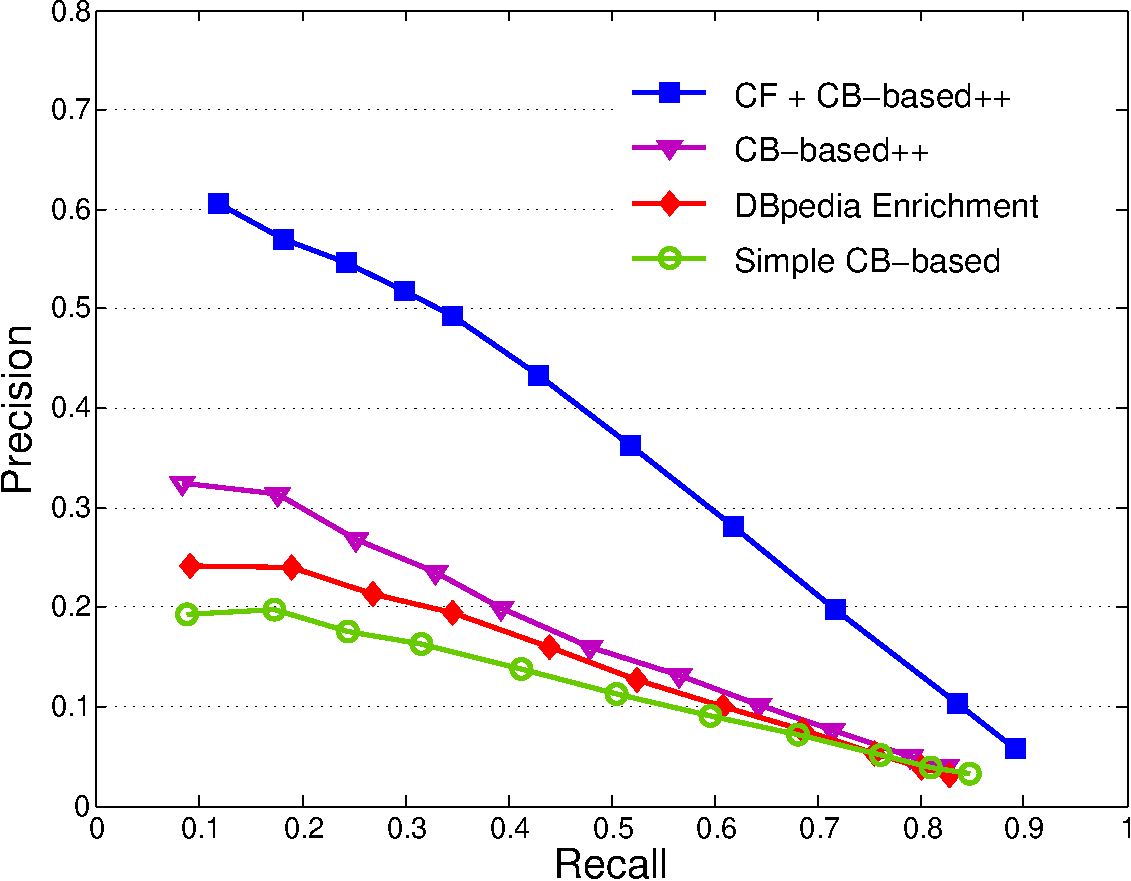
\includegraphics[height=62mm,width=80mm]{case-comparison.pdf}
  \caption{Evolution of the recommendation accuracy by incorporating the DBpedia enrichment, user diversity (CB-based++) and collaborative filtering (CF) }
  \label{fig:case-comparison}
\end{figure}

Lastly, we assess the extent to which a hybrid event recommendation outperforms the existing collaborative filtering based on matrix factorization to detect latent factors from the user-item matrix. We compare our system with the traditional user-based CF and the Probability based Extended Profile Filtering (UBExtended) proposed by Pessemier et al.~\cite{Pessemier:MTA12} to recommend events. This method employs a cascade of two user-based CF systems aiming to recommend the most consumed (i.e. popular) events. The rationale behind is that the probability to consume an event is proportional to the current popularity of the event (i.e. has attracted many users). The comparison results are depicted in Figure~\ref{fig:approaches-comparison}. It is shown that the UBExtended method outperforms the user-based CF algorithm. Still, the hybrid recommendation exhibits the best results in terms of precision and recall. This is due to the benefits of hybridization as has been highlighted in other research studies~\cite{Rojsattarat:2003}.

\begin{figure}[H]
  \centering
  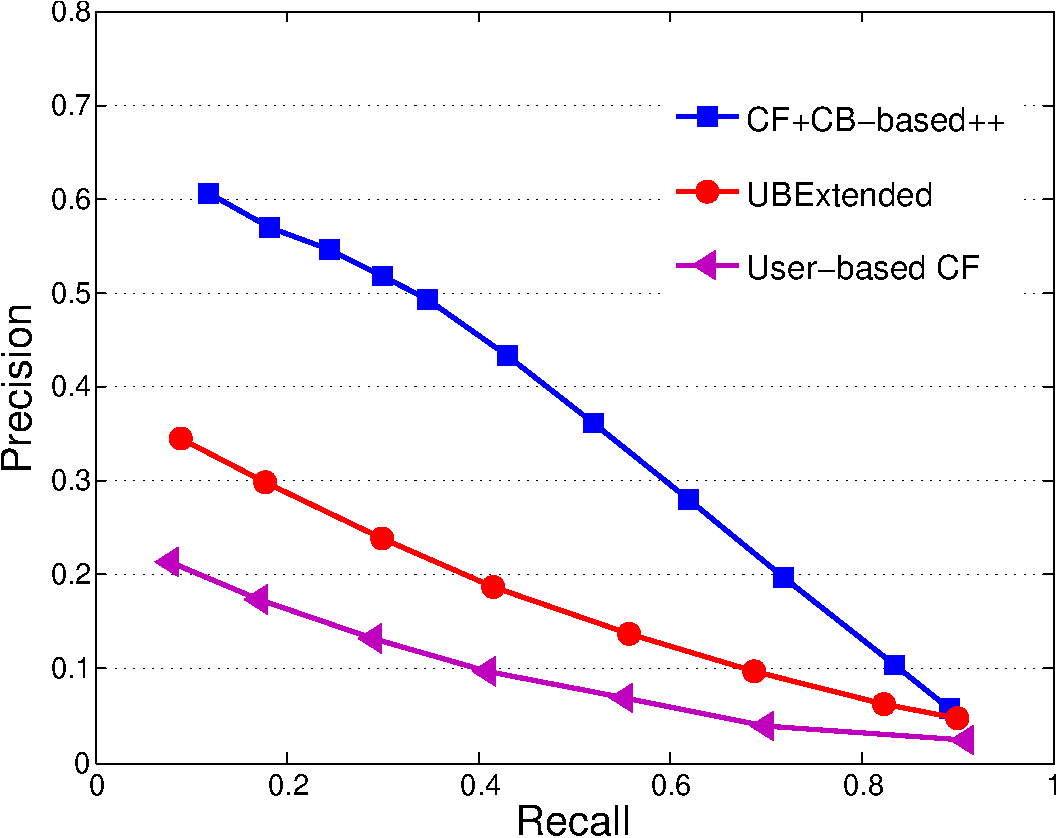
\includegraphics[height=62mm,width=80mm]{approaches-comparison.pdf}
  \caption{Comparison of hybrid event recommendation with pure CF algorithms}
  \label{fig:approaches-comparison}
\end{figure}

\section{Related Work}
\label{sec:related-work}
In the research area of recommender systems, many approaches have been proposed to recommend movies, but few are the studies that deal with event recommendation. Events are particularly hard to recommend due to their short life time and the system often suffers from high sparsity of rating data. Some works have been proposed to overcome these issues and improve the recommendation accuracy. Cornelis et al.~\cite{Cornelis:IICAI05} built a hybrid approach within a fuzzy relational framework that reflects the uncertain information in the domain. The rationale behind is to recommend future events similar to those like-minded users have liked in the past. However, this framework was not evaluated and there is no clear insight about its performance. Minkov et al.~\cite{Minkov:CIKM10} followed the same rationale and proposed a low rank collaborative method to predict the rating of future events. They highlight the performance of the collaborative filtering over the content-based system. Still, their approach was more tailored to recommend scientific talks in the same building and there is no consideration of the geographical constraint. Some other systems have been developed such as ``Pittcult''~\cite{Lee:RecSys08} and ``Eventer''~\cite{Kayaalp:ASONAM09} that position the user within a social network and leverage the trustworthiness between users. Such feature is valuable for recommendation, but it is not available in many systems. Finally, a user centered evaluation~\cite{Dooms:RecSys11} showed that the straightforward combination of CF and CB recommendations outperforms both individual algorithms on almost qualitative metrics such as accuracy, novelty, diversity, satisfaction and trust. Another interesting related works are the recent studies that harness the power of Linked Data in recommender systems. In~\cite{DiNoia:SEMANTICS12}, Di Noia et al. use the Linked Data as the only background knowledge to recommend movies. They highlight the performance of the system that exploits ontology-based data representation compared with the keyword-based representation. Still, there is no deep exploitation of the latent similarity that may exist between movie attributes (e.g. two similar actors).

\section{Conclusion}   \label{sec:conclusion}
In this chapter, we presented an approach for event recommendation combining both CB and CF advantages, and using Linked Data to enrich the event profile. In addition, we proposed an approach to model the user interests and to overcome the topical diversity in the user profile. The evaluation particularly highlights the importance of social information and the user diversity model to enhance the system performance. In the future, we plan to take into account other significant features such as event popularity and temporal indexing of recent consumption.

\chapter{Topical Community Detection in Event-based Social Network}  \label{ch:community-detection}
\graphicspath{{Part2/Chapter3/figures/}}

Websites such as   Lanyrd, Last.fm, Flickr and Twitter host an ever increasing amount of event-centric knowledge maintained by rich social interactions. In particular, there exists two types of \textit{Event-based Social Networks} (EBSN). The former is represented by the typical online activities such as sharing media and exchanging thoughts. The latter captures the face-to-face social interactions reflecting the offline co-participation in the same events. For example, in the academic conferences, researchers interact with other community members with whom they share common research background~\cite{Li:dasfa11a}. In other words, EBSN is a heterogeneous social network underlying the co-existence of both online and offline social links~\cite{Liu:KDD12}. Meanwhile, the information about these social interactions are spread over multiple websites. For example, people tend to mostly use media platforms (Flickr, Twitter) to share photos and thoughts about events, whereas they express their intent to attend events (RSVP) in online event directories (Eventful, Last.fm). Exploiting the overlap of these distributed websites is a key advantage to analyze the social networks. 

Community detection is considered as a major topic for analyzing social networks and has recently received a great attention. It aims to uncover the substructures within a network revealing which users are likely to have common interests, occupations and social properties. The information about the underlying communities can be of a great benefit for many tasks such as information diffusion and personalization. For instance, a personalization system can be based on user's community to gain more knowledge about his/her behavior~\cite{Shardanand:SIGCHI95,Paliouras:2012}. It has been also proved that the substructures within a network provide new powerful means of recommendation and collaborative filtering~\cite{Konstan:2012,Paliouras:2012}.


\section{Background} \label{sec:background}

Broadly speaking, detecting communities is dividing the vertices into groups such that there is a higher density of links within groups than between them~\cite{Clauset:PR04}. To achieve this, most of existing methods focus on network topology and structural properties. They assume that the interaction strength of users is the reflection of their proximity. However, communities detected by link-based methods often represent users having different interests since no consideration of the topical dimension was made. It is difficult to interpret the relationships of users grouped within such communities~\cite{Juan:cason11,Zhongying:12}. This problem becomes more important when users interact with objects related to diverse topics. Therefore, merging the semantic information with the linkage structure is essential in order to detect meaningful and interpretable communities. 

In EBSN, it is ideal to analyze the rich content about users and events in order to discover semantically coherent communities. Moreover, a person is naturally interested in many events which may be associated with multiple topics. It is thus more reasonable to divide users into overlapping topical groups instead of disjoint ones. Still, communities produced by topic-based methods may contain weakly connected users. They do not consider the relationships between users which results in significant loss of social information. An efficient community detection algorithm should cluster individuals who are closely connected and share common topics. 

In this chapter, we propose a novel approach to detect topical communities (i.e group of users sharing a common topic) by combining event clustering with link analysis. First, we compute the similarity of events based on the social information and the content attributes. Then, we use a hierarchical clustering to group events into different topics. Finally, a link-based function is defined to determine the effective user attachment to each community. 

%%%%%%%%%%%%%%%%%%%%%%%%%
%%%  2. Related Work  %%%
%%%%%%%%%%%%%%%%%%%%%%%%%
\section{Related Work} \label{sec:related-work-com}
Community detection has attracted attention in recent years leading to several interesting studies. Most of existing works attempt to detect disjoint communities by optimizing different link-based objectives. One popular example is the modularity optimization~\cite{Clauset:PR04,Newman:04} used to maximize the connectivity between nodes within one community and minimize the connectivity between groups. Another example is the minimization of a defined cut function in spectral methods~\cite{Scott:05}. These works mostly focused on structural properties and linkage patterns of people and they have been successfully used in some applications. However, they generally produce communities associated with different semantic topics.

To overcome the limitation of link-based methods, some studies attempt to exploit topic modeling techniques such as pLSA~\cite{Thomas:99}, LDA~\cite{Blei:MLR03} and AT (Author-Topic Model)~\cite{Steyvers:kdd04} used to detect topical communities. For example, the work in~\cite{Li:2013} made an analogy between the LDA document-topic-word and the user-topic-websites. The idea behind is that users sharing similar online access pattern tend to belong to the same topical group. This method primarily relies on the link information in a social graph, and it is only efficient when regular interaction patterns can be detected. Another technique called Community-User-Topic (CUT)~\cite{Zhou:WWW06} extends the LDA model to detect communities using the semantics of content. As a result, communities are represented as random mixtures over users who are associated with a topical distribution. This method does not consider the link information assuming that community members only share  common topics. Obviously, both methods can not be applied in real-world social networks where users' memberships are conditioned on their social relationships as well as their shared interests~\cite{Zhongying:12}.

Recently, some works start to investigate the combination of both content and link information. For example, the generative Bayesian model (Topic User Recipient Community Model) presented in~\cite{Sachan:WWW12} combines discussed topics, interaction pattern and network topology to detect topical communities. In~\cite{Zhongying:12}, Zhao et al. proposed an approach based on a modified k-means algorithm (EWKM-Entropy Weighting K-means) to partition social objects (e.g. mails, events, etc). into topical clusters. Each topical cluster contains members who interacted with the associated social objects. Then, a modularity maximization method is employed in each topical cluster to detect strongly connected communities. In our work, we made analogy between these social objects and events and we extensively compare our algorithm with this approach (called EWKM-based method in the following). 

The last concern in related work is the research on discovering communities in EBSN. Liu et al.~\cite{Liu:KDD12} addressed the problem of community detection in heterogeneous network. Their approach is based on an extended Fiedler method to consider both the online and offline social interactions. This method seems efficient to detect cohesive communities, but it is still a link-based method and no interpretation of detected communities was made. In~\cite{Li:dasfa11a}, the Event-based Community Detection (ECODE) algorithm enriched the network with virtual links based on content-based users' similarity. Virtual links aim to enhance connectivity among individuals sharing common topics (e.g. content). A hierarchical clustering is then used to group events based on their physical and virtual similarity. In the same context, Wang et al.~\cite{Wang:14}, proposed a community detection approach in location-based social network (LBSN). Their approach exploits different features such as user social similarity and venue-user similarity, and uses an edge-centric co-clustering which simultaneously discovers overlapping groups of venues and that of users. To sum up, these different studies provide important insight into detecting communities in EBSN. However, none of them aims to maximize both connectivity strength and topical purity within communities.


%%%%%%%%%%%%%%%%%%%%%%%%%%%%%%%%%%%%%%%
%%%  Event-based Social Network  %%%
%%%%%%%%%%%%%%%%%%%%%%%%%%%%%%%%%%%%%%%
\section{Event-based Social Network} \label{sec:esbn}
In this section, we describe how to construct an event-based social network using offline and online interactions (Section \ref{sec:esbn-def}) and we highlight some of their interesting properties (Sections \ref{sec:spatial-aspect} and \ref{sec:network-prop}).

\subsection{EBSN Definition}   \label{sec:esbn-def}

Based on user activities in social services, we define the following EBSNs making difference between online and offline networks. Slightly different from the definition given by Liu et al.~\cite{Liu:KDD12}, we consider that the online EBSN is constructed by solely capturing the online interactions such as sharing comments and photos about events. This online EBSN is different from the online ``friendship'' social network that may exist in some services as defined in~\cite{Liu:KDD12}. Similarly, the offline EBSN is constructed by considering the physical co-participation in social events.

\vspace{2mm}
\begin{itemize}
\item \textbf{Event Directory}
	\begin{itemize}
	\item {\textbf{Last.fm EBSN.}} In Last.fm, there are two networks: the online EBSN is built based on the online co-commenting of social events, whereas the offline 		EBSN is based on the explicit RSVP provided by users.
	\end{itemize}

\item \textbf{Media Directories}
	\begin{itemize}
	\item {\textbf{Flickr EBSN.}} Flickr is one of the most important online photo sharing websites. Thus, we exploit the activity of co-sharing photos related to the same events to build an online media EBSN.

	\item {\textbf{Twitter (Lanyrd) EBSN}} Twitter is a popular micro-blogging service, and it is by far the most used back-channel for commenting scientific conferences~\cite{Khrouf:RAMSS12}. Similarly, we exploit the co-commenting activity about the same conferences to build another online media EBSN.
	\end{itemize}
\end{itemize}


\subsection{Spatial Aspect of Social Interactions}   \label{sec:spatial-aspect}
In the following, we investigate how far from their homes people interact within the offline and online EBSNs. Therefore, we compare the geographical distance between an event location and the user's home. However, as the user's home location is not explicitly provided by Last.fm, we infer it using the average of most frequent positions of attended events. Results are depicted in Figure~\ref{fig:event-user-distance} based on a random set of events and their associated users.

We observe that 95\% of users' activities in offline network are within 100 km. This rate slightly decreases in online Last.fm EBSN indicating that people tend to also comment nearby events. This aspect has already been proved in an existing study~\cite{Liu:KDD12} showing that users' activities in EBSNs are much more location constrained compared with location-based social network. In contrast, the online interactions in media-based EBSNs seem to be less conditioned on event location. The reason behind can be two-fold: (1) the nature of sharing activity which is more present in media platforms than event directories, and the users are generally non-uniformly spread; (2) the type of events indicating that people tend to travel far from their home for business purpose (conference) rather than for entertainment activity (musical concert).  

\begin{figure}[H]
  \centering
  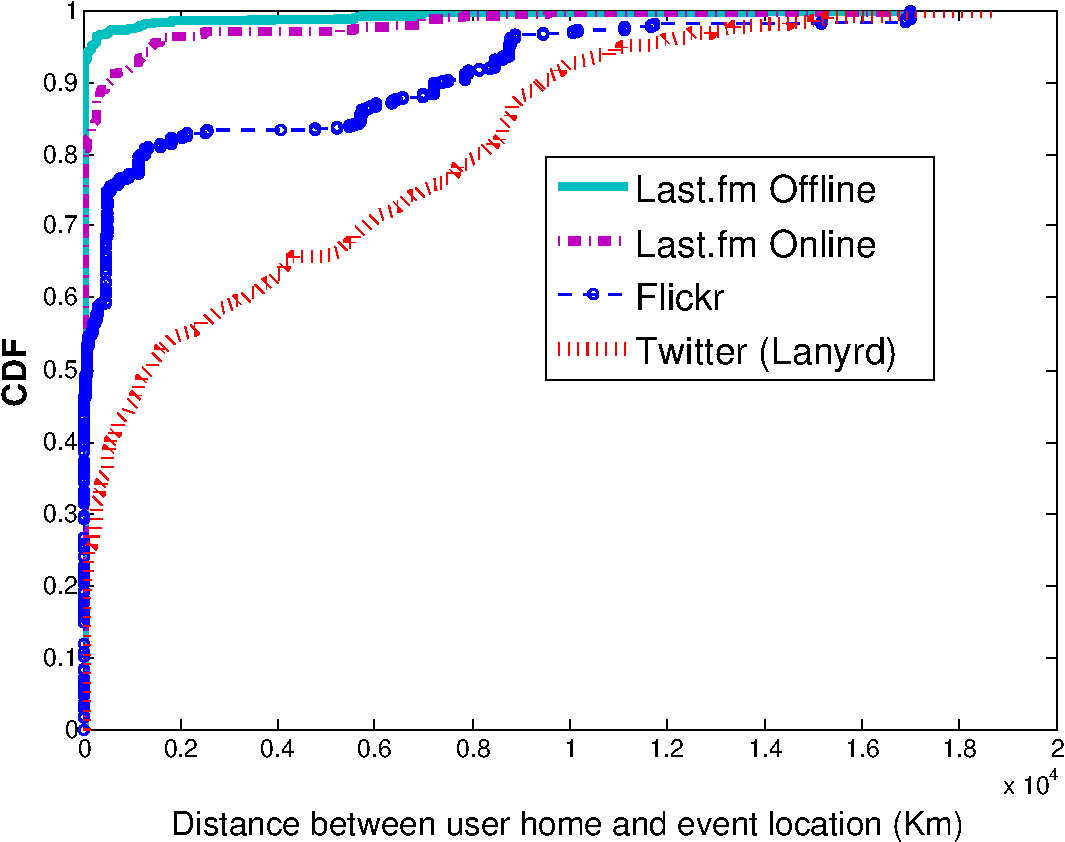
\includegraphics[scale=0.5]{location-participation.pdf}
  \caption{Locality of user activities in offline and online EBSNs}
  \label{fig:event-user-distance}
\end{figure}

Based on these findings, we decided to perform community detection using conferences from different cities in Lanyrd, whereas we only focus on a specific geographical location in Last.fm. 

\subsection{User Participation}   \label{sec:network-prop}

\begin{figure}[htb]
\centering
\subfigure[]{\label{fig:users-events_a}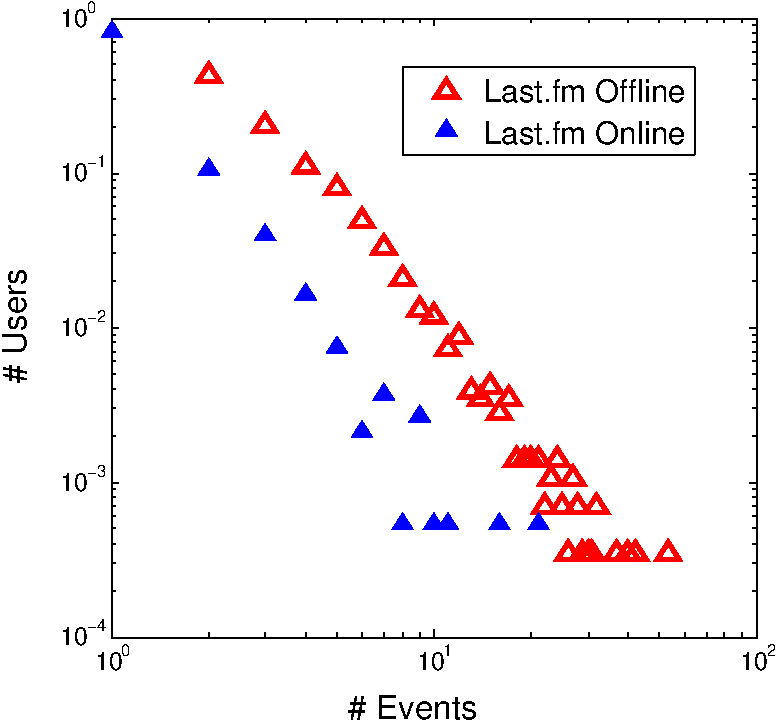
\includegraphics[height=60mm,width=67mm]{users-events-1.pdf}}
\subfigure[]{\label{fig:users-events_b}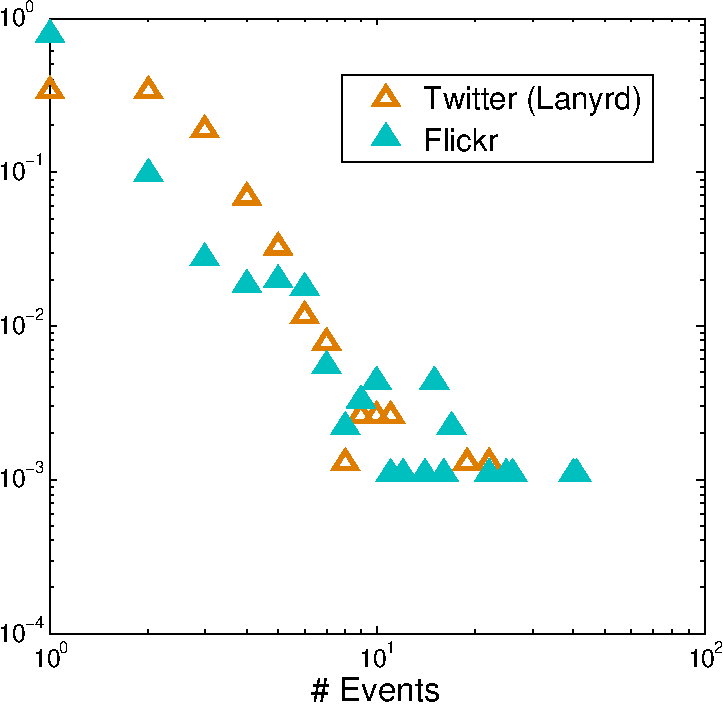
\includegraphics[height=60mm,width=63mm]{users-events-2.pdf}}
\caption{Number of participants per event in (a) Last.fm offline and online EBSN and (b) Flickr and Twitter online EBSN}
\label{fig:users-events}
\end{figure}

To gain insight into some EBSN properties, we study the user participation behavior. As shown in Figure~\ref{fig:users-events}, the results resemble a power-law distribution indicating that most of users are associated with few events. Similar results have been highlighted in other works studying the event attendance behavior~\cite{Liu:KDD12,Han:NCWTW12}. In particular, there are 81\% of users who are associated with only one event in Last.fm online EBSN, and 76\% of users sharing photos of only one event in Flickr EBSN (this can be drawn from Table~\ref{tab:dataset-stats} if we compare the number of media shared with the number of users). During the evaluation, we will show the influence of the user participation distribution on community detection.    


%%%%%%%%%%%%%%%%%%%%%%%%%%%%%%%%%%%%%%%%
%%%  4. Topical Community Detection  %%%
%%%%%%%%%%%%%%%%%%%%%%%%%%%%%%%%%%%%%%%%
\section{Topical Community Detection} \label{sec:community}
In this section, we first describe our graph model (Section~\ref{sec:modeling}). Then, we present our approach proposed to detect topical communities. 

%%%%%%%%%%%%%%%%%%%%%%%%%%
%%%  5.1 Graph Modeling %%%
%%%%%%%%%%%%%%%%%%%%%%%%%%
\subsection{Graph Modeling}  \label{sec:modeling}
Taking into account the users, the events and their related attributes, we consider the fourth-tuple graph $G=<U,S,T,E>$ for both online and offline EBSN where $U$ is the set of users, $S$ is the set of social events which are in turn associated with a set of tags, and finally $E$ is the set of undirected edges. $E$ contains two kinds of links $E=E_{US} \cup E_{UU}$:
\begin{itemize}
\item $E_{US}$ denotes the links between users and social events, formalized as $E_{US}={\lbrace(u,s)| u \in U,s \in S \rbrace}$
\item $E_{UU}$ is the set of links between users (i.e. a link represents the co-participation in same social event), formalized as $E_{UU}={\lbrace(u_{i},u_{j})| u_{i} \in U,u_{j} \in U \rbrace}$. 
\end{itemize}

In this graph, each user can be represented as a vector of events, and each event can be represented as a vector of users. Similar way is applied using the event-tag relationship. We exploit these representations to compute the similarity of events which will be used for detecting communities.

\subsection{The Proposed Approach}   \label{sec:approach}
In our approach, we follow the same rationale as the EWKM-based method proposed by Zhao et al. ~\cite{Zhongying:12}. The idea behind is to group together the social objects which share the same topic, and  . Then, users within each cluster are divided into sub groups using the modularity maximization. Instead of performing two-step clustering, we propose one step clustering taking into account both the link and content information. 

%%%%%%%%%%%%%%%%%%%%%%%%%%
%%%  5.2 Similarity Computation %%%
%%%%%%%%%%%%%%%%%%%%%%%%%%
\subsubsection{Similarity Computation}  \label{sec:similarity}
In EBSN, the overlapping communities of users who share common interests can be detected by clustering similar events together~\cite{Li:dasfa11a}. Given the large number of users, we assume that event-based clustering have a less computational time compared with user-based clustering.  Still, the event similarity should reflect both the link and content information in order to discover topical communities. To solve this, we use the notion of \emph{Homophily} which is observed in many social networks~\cite{McPherson:2001}. Homophily refers to the tendency of persons to be associated with other persons that share similar characteristics. In other words, users involved in same events have a higher likelihood to share similar interests and get connected. Similarly, tags associated with same events are more likely to be topically similar. This implies that similar events are sharing both like-minded users and semantically similar tags. Thus, we cluster events based on their similarity both in the user space and in the semantic space.

In the event-user network, events can be represented as a vector of users, and users can also be viewed as a vector of events. To reduce the dimension of the event-user matrix, we need to represent events in a latent user space using an orthogonal basis. Singular Value Decomposition (SVD) is one popular technique employed to obtain such basis.  Given a matrix $A$, the singular value decomposition is the product  $U \Sigma V^T$ where $U$ and $V$ are the left and right singular vectors and $\Sigma$ is the diagonal matrix of singular values. Event vectors in the latent user space is represented by the matrix $\tilde{A}$ as follows:

\begin{equation}  \label{eq:event-latent}
\tilde{A}=U\Sigma \Rightarrow  \tilde{A}=AV
\end{equation}
In order to detect similar events that share like-minded users, we leverage the spectral co-clustering~\cite{Dhillon:KDD01} indicating that only the top singular vectors, except of the first one, contain partition information. The algorithm first normalizes the event-user matrix as follows: 

\begin{equation}  \label{eq:event-latent}
A_n=D_1^{-1/2} A D_2^{-1/2} 
\end{equation}
where the entries of the diagonal matrices $D_{1} $ and $D_{2}$ are respectively the event degrees and the user degrees (i.e. a degree is the number of connections the node has to other nodes). Then, applying SVD on $A_n$ gives $A_n=U_n \Sigma_n V_n^T$.  Only the top-k singular vectors (except of the first one) are selected from $V_n=(v_1, v_3,...,v_n)$ to form the matrix $V'_n=(v_2, v_3,...,v_m)$ where $m \ll n$. Finally, the event representation in the user latent space is shown in Equation~\ref{eq:event-latent-1}.

\begin{equation}  \label{eq:event-latent-1}
\tilde{A}=D_1^{-1/2} A_n V'_n
\end{equation}
Similarly, we represent events in the latent semantic space applying this method on the event-tag network. Recent experiments in text corpus suggests that the dimension $m$ of $V'_n$ depends on the corpus size and it was set between 50 and 1000~\cite{Landauer:2008}. Indeed, small value of $m$ is advantageous to remove noisy information. In our case, we set $m$ equal to 200 for the user space and equal to 50 for the semantic space (there are more users than tags in our dataset). Afterwards, we use Cosine distance to compute the events similarity $S_u$ in the latent user space and $S_t$ in the latent semantic space. Finally, we combine the similarities as follows:

\begin{equation}  \label{eq:event-sim}
S_{sim} =\alpha \ S_u + (1-\alpha) \ S_t
\end{equation}
where $\alpha$ is the parameter that controls the balance between user-oriented similarity and tag-oriented similarity. In this approach, the pair-wise computation using Cosine distance can be reduced by selecting candidate solutions that only index the potentially similar events. Intuitively, these solutions are the events that share in common a minimum number of tags or users with the original event. Variants techniques can be used such as the Locality Sensitive Hashing (LSH)~\cite{Gionis:VLDB99} or its variants (e.g. MultiProbe LSH~\cite{Lv:VLDB07}) which are popular high-dimensional similarity search methods. In ECODE algorithm~\cite{Li:dasfa11a}, it has been shown that the candidate selection was efficient to save a significant amount of computational time without affecting the communities detected. Although it can be easily applied, candidate selection is not considered in the present work since we deal with small datasets.

%%%%%%%%%%%%%%%%%%%%%%%%%%
%%%  5.3 Hierarchical Clustering %%%
%%%%%%%%%%%%%%%%%%%%%%%%%%
\subsubsection{Hierarchical Clustering} \label{sec:clustering}
Inspired by the ECODE algorithm~\cite{Li:dasfa11a} described in related work (Section~\ref{sec:related-work-com}), a hierarchical agglomerative clustering is used to group similar events in terms of correlated users and tags. Agglomerative clustering begins by assigning each data item to its own individual cluster. The two most similar clusters are merged together into a single cluster.  This step is repeated until all the items are grouped into a single cluster, thus forming a hierarchy (i.e. tree).

\begin{algorithm}
\caption{Agglomerative clustering of similar events}
\label{alg:clustering}
\begin{algorithmic}
\STATE S: set of social events $s_1, s_2...s_i$
\STATE T: number of topics
\STATE $S_{sim}$: event similarity matrix
 \WHILE {Community Size$>$T \And {\  } $SemQ$ function increases}
	   \STATE Merge the most similar events $s_i$ and $s_j$ into a new event $s_{new}$
 		\FOR {each event $s_k$ $\in$ S (or candidate set)}
 			\STATE $S_{sim}(s_{new},s_k)$ =  average($S_{sim}(s_{new},s_i)$+$S_{sim}(s_{new},s_j)$)
		\ENDFOR
\STATE Compute $SemQ$		
\ENDWHILE
\end{algorithmic}
\end{algorithm}

As outlined in Algorithm~\ref{alg:clustering}, the most similar events $s_i$ and $s_j$ are clustered together forming a new event $s_{new}$. Then, we compute the similarities between $s_{new}$ and each event in the dataset or in the candidate set (if the candidate selection is considered). Finally, the clustering stops when there is no significant increase of the quality function. This approach is advantageous compared with other algorithms such as k-means since the predefined number of clusters is not required.

To produce topical clusters, the quality function of the tree follows the same rationale than Newman modularity but applied on the semantic space. Indeed, our goal is to maximize the intra-similarities and minimize the inter-similarities in the semantic space. Thus, we define a novel function called \textit{semantic modularity}. To formalize this function, we use the events similarity  $S_t$ computed in the latent semantic space in order to compute the intra-similarities (IntraSem in Equation~\ref{eq:intra}) and inter-similarities (InterSem in Equation~\ref{eq:inter}) as following:

\begin{equation} \label{eq:intra}
       {IntraSem}=\frac{1}{|C|}\sum_{C_k \in C} \frac{\sum_{i,j \in C_k, i  C_i j } S_t(i,j)}{|C_k| (|C_k|-1)} 
\end{equation}

 \begin{equation} \label{eq:inter}
      {InterSem}=  \frac{1}{|C|} \sum_{i \in C_i} \frac{\sum_{j \in C_j,  C_i \ne  C_j} S_t(i,j)^2}{M}  
\end{equation}
where C is the set of discovered clusters, and M is the number of comparisons made in inter-similarities. Finally, the semantic modularity $SemQ$ is defined as following:

 \begin{equation} \label{eq:quality}
		SemQ=IntraSem-InterSem
\end{equation}

Note that the maximal $SemQ$ provides the topical clusters of events and stop the clustering process. In meanwhile, each detected cluster keeps in mind a minimal knowledge about the link information held by the event similarity in the user space, which makes our approach different from the EWKM-based method~\cite{Zhongying:12}. 

%%%%%%%%%%%%%%%%%%%%%%%%%%
%%%  5.4 User Assignment %%%
%%%%%%%%%%%%%%%%%%%%%%%%%%
\subsubsection{User Assignment}   \label{sec:assignment}
The last step of our approach is to group together users associated with each cluster by simply using the user-event links.  As the user may participate in many events, we can generate overlapping topical communities. However, a user may be weakly involved in one topical cluster that not really reflects his/her interests. To address this problem, we propose to discover the effective user's memberships by computing his/her assignment scores. If the user $u_i$ is a member of the community $C_i$, the assignment function is defined as follows:

\begin{equation}    \label{eq:assignment}
			AS(u_i,C_i)=\frac{D_c(u_i)}{D(u_i)}				
\end{equation}
where $D_c(u_i)$ is the degree of the user $u_i$ within the community $C_i$ (i.e. number of links of the user with other community members), and $D(u_i)$ is the global $u_i$'s degree. The user's membership to one community is determined if the related assignment score is higher than the average of non-zeros scores over all communities. Note that the user assignment method based on Equation~\ref{eq:assignment} may convert a cluster to an empty one. We believe that the removal of these empty clusters is reasonable since they represent groups of very weakly connected users.

%%%%%%%%%%%%%%%%%%%%%%
%%%  5. Experiments and Evaluation %%%
%%%%%%%%%%%%%%%%%%%%%%
\section{Evaluation}   \label{sec:experiments}
This section presents the evaluation of the proposed community detection approach applied on real-world datasets. We first describe these datasets  followed by the description of the performance metrics and the obtained results.

%%%%%%%%%%%%%%%%%%%%%%%%%%%%%%%%%%
%%%  5.1 Experimental Datasets %%%
%%%%%%%%%%%%%%%%%%%%%%%%%%%%%%%%%%
\subsection{Experimental Datasets}
Based on the definition of online and offline EBSNs, we use the following datasets placed online\footnote{\url{http://www.eurecom.fr/~khrouf/esbn}} (some statistics are shown in Table~\ref{tab:stats}).

\begin{itemize}
\item \textbf{Entertainment (Last.fm and Flickr):} We previously demonstrated that a very high fraction of social interactions for entertainment purpose  exist between geographically close friends. Hence, we focus our analysis on events located in one city. The capital ``London'' has been selected since it exhibits a significant number of users and events compared with other cities in EventMedia. Operationally, we query the EventMedia SPARQL endpoint to retrieve data, and we crawl additional metadata using the REST API of Last.fm and Flickr. Then, we pre-process the dataset as follows: First, we remove the tags associated with very low frequency (less than 5) to reduce the topical noise, and we only keep the events which are associated with the frequent tags (musical genres). Second, we remove the singletons of event-user pairs where the event has only one participant, and this participant is associated with only one event. We retrieve the events happened in 2012 and 2013 (associated with media) and we obtain the following EBSNs: (1) an offline Last.fm EBSN containing 915 events, 2847 users and 272 tags; (2) The associated online Last.fm EBSN contains 470 events (among 915 events), 1729 users and 248 tags (among 272 tags); (3) The associated online Flickr EBSN contains 375 events, 868 users and 221 tags. Note that the removal of singletons event-user pairs has significantly reduced the size of the online Last.fm and Flickr EBSNs indicating that users' activities in those networks are more sporadic and mostly present individual behaviors.

\item \textbf{Conference (Lanyrd and Twitter)} Similarly, we use SPARQL queries to retrieve data from EventMedia along with the Twitter API for additional information (e.g. user's home location). Note that Lanyrd also provides details about the conference attendees, but this information was missing in EventMedia at the time of writing. Thus, we plan to further enrich our dataset and we left the analysis of offline Lanyrd EBSN for future study. Then, we pre-process the data retrieved as follows: As no tags were associated with events, we automatically process the conference description (tokenization, stop-words removal, etc.). However, this method produced very noisy tags because some conferences are vaguely described (e.g \emph{The World is Changing, Is Your Company on Board?}).  We also attempt to automatically process the tweets. Still, many tags do not really reflect what is the conference about due to the presence of several noisy tweets (e.g. personal status updates, opinions, etc.). As an alternative solution, we manually label the conferences descriptions by selecting the most representative keywords. Due to the manual effort, we only keep the interesting conferences which are related with very active users. Finally, we obtain an online EBSN which contains 275 events, 768 Twitter users and 166 tags. Note that there is a small set of events compared with Last.fm EBSN due to the high selectivity followed.
\end{itemize}
\begin{table}[H]
\centering{
\begin{tabular}{cccc}
\hline
& Edges & Density & ClustCoeff \\
\hline
Last.fm Offline & 95897 & 0.0237 & 0.1144\\
\hline
Last.fm Online & 9936 & 0.0067 & 0.398\\
\hline
Flickr Online &  7071 & 0.0188 & 0.2624 \\
\hline
Twitter Online & 14237 & 0.0483  & 0.4852 \\
\hline
\end{tabular}
\caption{Some statistics about the datasets}
\label{tab:stats}
}
\end{table}

\subsection{Topic Modeling}
In order to assess the topical purity in each cluster, we first need to detect the set of topics in each dataset. Thus, we decided to employ LDA~\cite{Blei:MLR03}, a popular topic modeling technique where we consider the events as documents. The use of LDA has led to coherent topics in Lanyrd dataset, but slightly ambiguous topics in Last.fm datasets. We explain this difference by the manual labeling in Lanyrd dataset where we carefully select qualitative tags. In contrast, Last.fm contains crowdsourced tags generated without moderator oversight and known to be less accurate. Moreover, the musical concerts may feature many artists related to different genres (i.e topics) or only one genre, making more difficult to detect co-occurrences. The conferences, on the other hand,  often target only one major topic (e.g. Semantic Web). 

To solve the topic modeling in Last.fm, we resolved to exploit the classification of musical genres that may help detect the fuzzy similarity between them (e.g. death metal and deathcore). More precisely, we leverage the existing SKOS taxonomy\footnote{\url{http://dbpedia.org/page/Category:Musical_subgenres_by_genre}} in DBpedia using the generalization relations such as \texttt{skos:broader} and \texttt{skos:narrower}. Tables \ref{tab:topics-lanyrd} and \ref{tab:topics-lfm} show few examples of topics detected respectively in Lanyrd and Last.fm. Note that we obtained 24 topics in Last.fm consisting of high-level musical genres, and 30 topics in Lanyrd where the optimal number of topics is determined based on the approach proposed by Griffiths et al.~\cite{Griffiths:04}. Finally, Figure~\ref{fig:event-topic} shows that many conferences have at most two topics, while this number slightly increases in musical events. 

\begin{table}[H]
\centering{
\begin{tabular}{c|c}
\hline
    \textbf{Topic}       &  \textbf{Example of Lanyrd Tags}  \\
\hline
   Education  &   learning, education, teaching, technology\\
\hline
   programming  &   programming, language, python, library\\
\hline
   Innovation  &   creativity, technology, business, future\\
\hline
   Application  &   mobile, application, web \\
\hline
\end{tabular}
\caption{Example of topics detected in Lanyrd}
\label{tab:topics-lanyrd}
}
\end{table}

\begin{table}[H]
\centering{
\begin{tabular}{c|c}
\hline
    \textbf{Topic}       &  \textbf{Example of Last.fm Tags}  \\
\hline
   Heavy metal  &   metal alternative, progressive metal... \\
\hline
   Pop  &   synthpop, powerpop, pop punk...\\
\hline
   Electronic  &   indietronica, synthpop, folktronica...\\
\hline
   Rock  &    hard rock, alternative rock, glam rock... \\
\hline
\end{tabular}
\caption{Example of topics detected in Last.fm}
\label{tab:topics-lfm}
}
\end{table}


\begin{figure}[H]
  \centering
  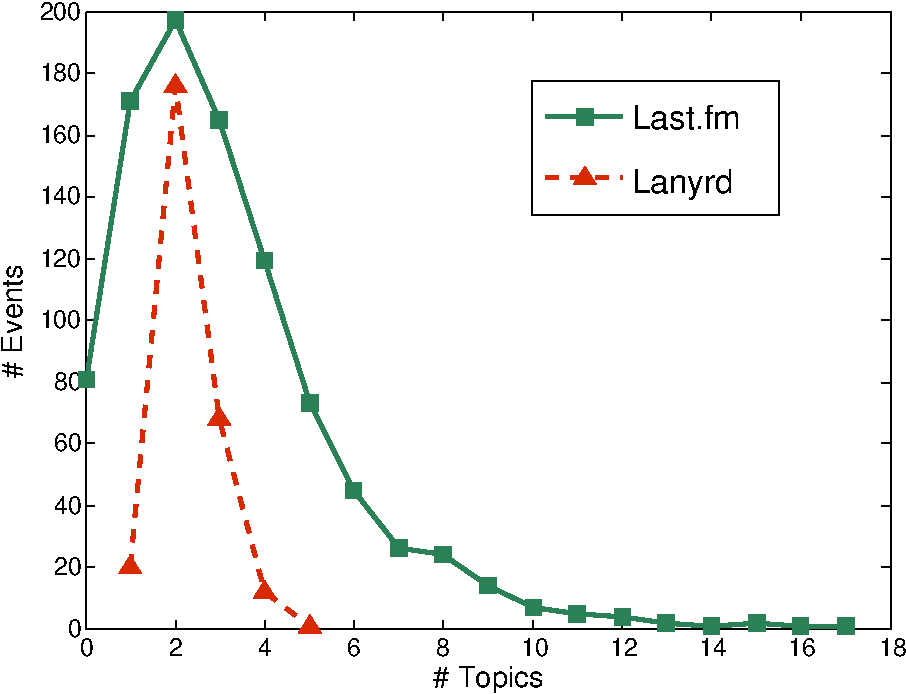
\includegraphics[scale=0.5]{topic-distrib.pdf}
  \caption{Histogram of the number of topics per event}
  \label{fig:event-topic}
\end{figure}


%%%%%%%%%%%%%%%%%%%%%%%%%%%%%%%
%%%  5.2 Performance Metrics %%%
%%%%%%%%%%%%%%%%%%%%%%%%%%%%%%%
\subsection{Evaluation Metrics}
To evaluate our approach, the performance metric should take into account the combination of both content and link information. We adopt the $PurQ_\beta$ metric introduced by Zhao et al.~\cite{Zhongying:12}. It has been inspired by the F-score measure that considers both the precision and the recall metrics. $PurQ_\beta$ considers both the topical purity and the members connectivity. First, we introduce the function that measures the topical purity in each cluster as following:

\begin{equation}    \label{eq:purity}
     Purity_i= max_j \left( \frac{n_{ij}}{n_i} \right)
\end{equation}
where $n_{ij}$ is the number of tags belonging to topic $j$ and cluster $i$, and $n_i$ is the number of tags in the cluster $i$. The final score of $Purity$ is the overall average of all the purity scores. Yet, we observed during the experiments that Purity does not effectively reflect the presence of clusters having low topical purity. Hence, we decided to also examine the $F_{purity}$ which is the faction of clusters having $Purity_i$ higher or equal than the average $Purity$. Finally, the metric $PurQ_\beta$ combining the content and link information is:


\begin{equation}    \label{eq:purq}
	PurQ_\beta= \frac{(1+\beta^2) (Purity \cdot Q )}{\beta^2 Purity + Q}			
\end{equation}
where $Q$ is the Newman modularity~\cite{Newman:04} used to evaluate the goodness of a partition, ensuring that there are many edges within communities and only a few between them. Then, the parameter $\beta$ is used to adjust the weight of $Purity$ and $Q$. $\beta=0.5$ means that $PurQ_\beta$ puts more emphasis on $Purity$ than $Q$. In contrast, $\beta=2$ puts more emphasis on $Q$. The general behavior of communities is when $Purity$ increases, $Q$ decreases, and vice versa.


%%%%%%%%%%%%%%%%%%
%%%  Results    %%%
%%%%%%%%%%%%%%%%%%

\subsection{Results} 
We first evaluate how the coefficient $\alpha$ in Equation~\ref{eq:event-sim} affects the performance of our approach. Figure~\ref{fig:alpha-impact} shows the evolution of the $Purity$ and the modularity $Q$ when $\alpha$ increases. It can be seen that the modularity increases if a high weight is assigned to event similarity in the user space. However, the purity and the modularity do not evolve at the same scale. While $Q$ slightly increases, $Purity$ drastically decreases. Thus, good values of $PurQ_\beta$ can be obtained when $\alpha \in $[0.1,0.5]. 

Then, we compare our approach with some related works: (1) Edge co-clustering (or EdgeCluster) inspired by the approach applied on the location-based social network and proposed in~\cite{Wang:14}. For this approach, we consider as features the user similarity in the event space and in the semantic space. Based on these features, Edge co-clustering uses k-means to cluster similar ``user-event'' edges. This method was evaluated only on two datasets as it requires a very large computation time; (2) ECODE algorithm which introduces the concept of content-based virtual links in the user-event graph and clusters together similar events sharing high physical and virtual links; (3) The popular Newman Modularity maximization (link-based method); (4) The EWKM-based method as detailed in related work (Section~\ref{sec:related-work-com}).

\begin{figure}[htpb]
  \centering
  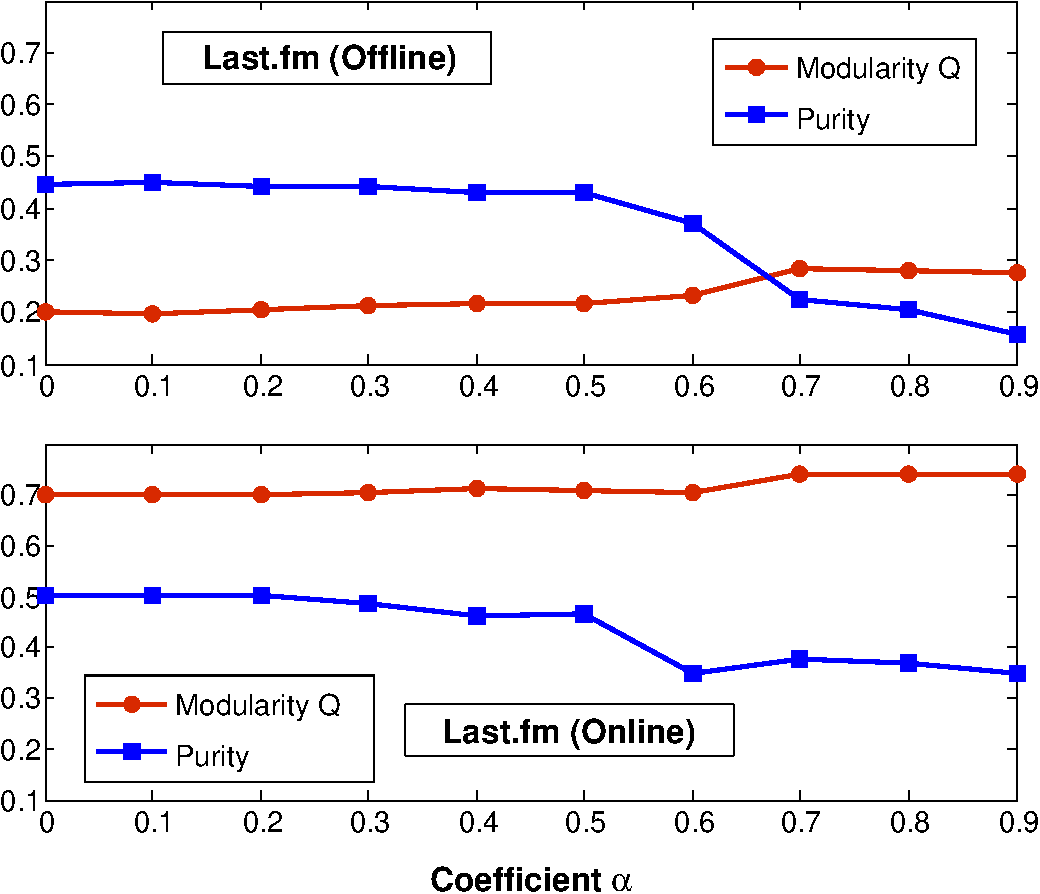
\includegraphics[scale=0.42]{alpha-performance.pdf}
  \caption{The evolution of Q and Purity with $\alpha$}
  \label{fig:alpha-impact}
\end{figure}

\begin{figure}[htbp]
  \centering
  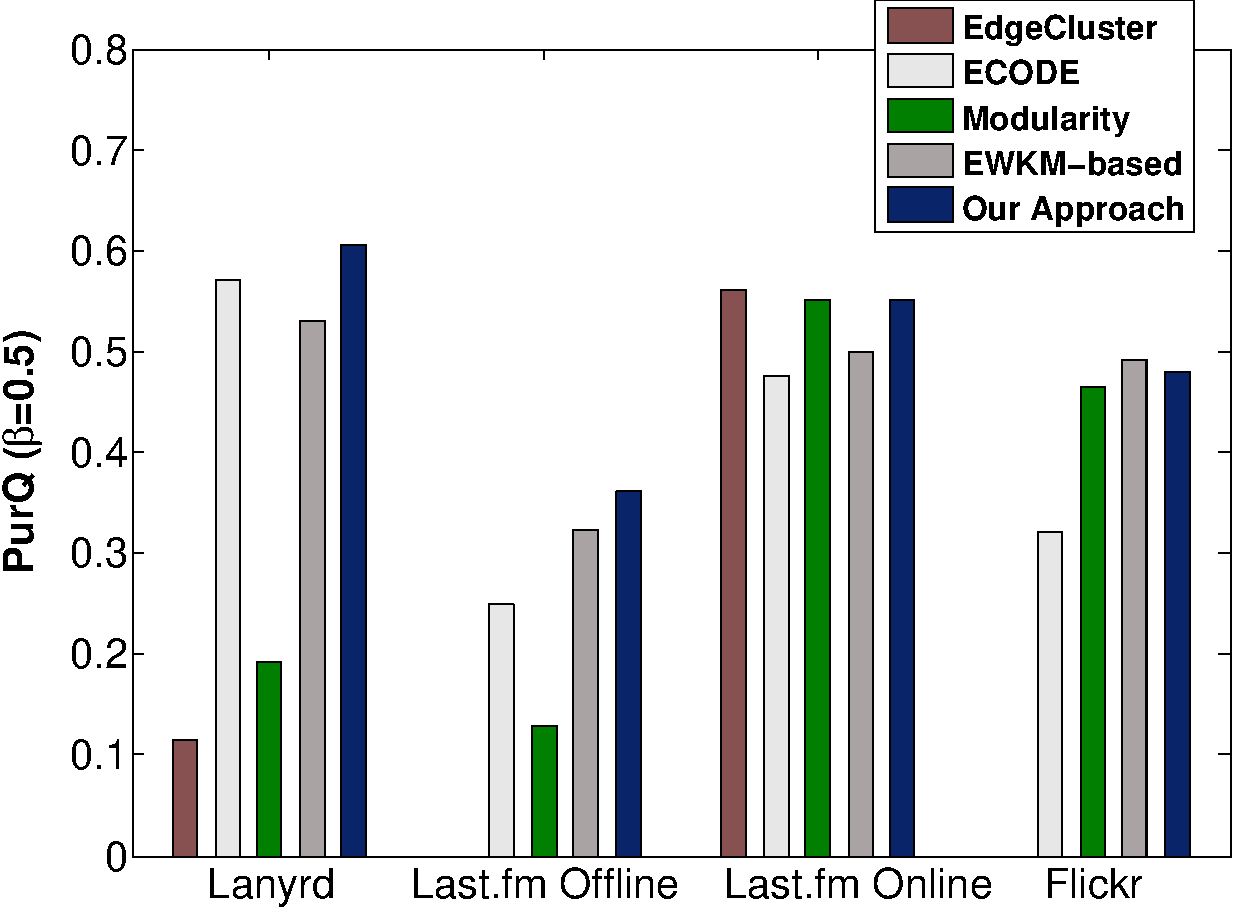
\includegraphics[scale=0.35]{PurQ-05.pdf}
   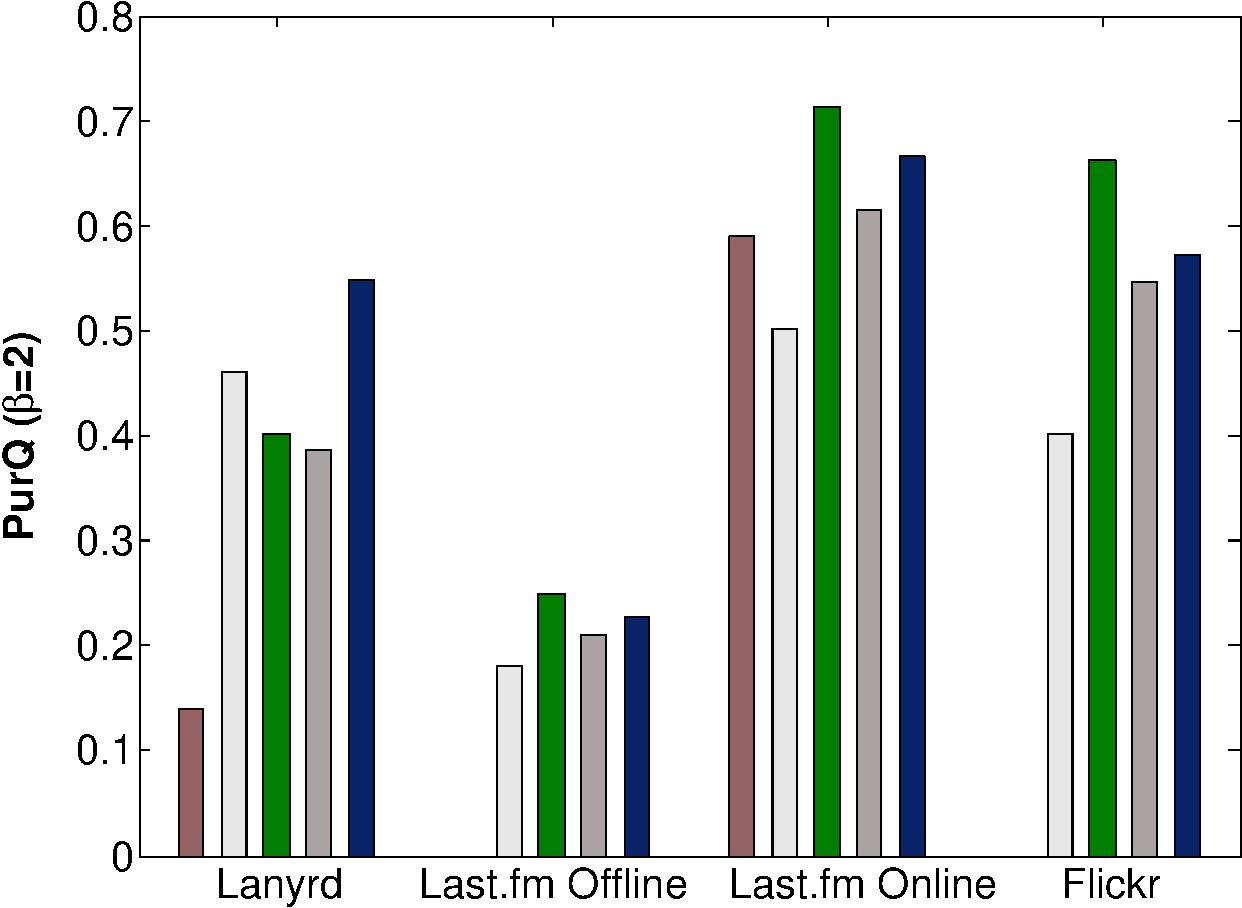
\includegraphics[scale=0.35]{PurQ-2.pdf}
  \caption{The performance comparison with $\beta=0.1$ and $\beta=2$ for different datasets}
  \label{fig:PurQ}
\end{figure}


The comparison results are depicted in Figure~\ref{fig:PurQ}. All these methods have nearly similar performance in Last.fm Online EBSN particularly when $\beta=0.5$. Indeed, the communities detected within this network have very small sizes (e.g average size equal to 15 for the Modularity method) due to the extremely sporadic interactions. This is also explained by the low density link and the user participation behavior where 92\% of users are associated at most with only two events. Hence, the link information was sufficient to obtain a good purity. This aspect slightly decreases in Flickr dataset where 78\% of users are associated with at most two events. The Modularity method apparently achieves a good purity. However, the fraction $F_{purity}$ is only equal to 0.6, a fair value compared with EWKM-based method and our approach where $F_{purity}$ are respectively equal to 0.89 and 0.91. In Last.fm Offline and Twitter EBSNs, the Modularity method has a poor performance when $\beta=0.5$. This can be explained by the network density which is high in those datasets compared with others. Moreover, the identified communities are very large. For example, we found an average size of 474.5 in the communities produced by the Modularity method in Last.fm offline EBSN. This indicates that users within this network are densely linked which can justify the low $Q$ values produced by different approaches. 


Evaluating the content-based methods, we note a better performance for ECODE in Twitter EBSN than in the other datasets. This is due to the addition of virtual links to the graph based on the content-similarity between users. However, the user profile in Last.fm is much more topically diverse than in Lanyrd which leads to ambiguous similar scores. In reality, the user may be interested in many musical concerts having different topics, whereas he has more restrictive ``scientific'' interests that mostly fit his/her expertise domain. We also observe a poor performance of the Edge co-clustering algorithm in Twitter EBSN because it is sensitive to the number of clusters that needs to be accurately determined. Finally, our approach achieves the best performance both when $\beta=0.5$ and $\beta=2$. Note that there is similar behavior between our method and the EWKM-based method. For instance, the average size of communities in Last.fm Offline EBSN is equal to 0.33 for EWKM-based, and 0.29 for our approach. However, the EWKM-based method is based on k-means clustering which is sensitive to the initial distribution of centroids, thus producing different results in each run. This problem is absent in our approach which is based on hierarchical clustering. From the computation point of view, we observe that all methods have nearly the same computational time except of the Edge co-clustering method. Finally, low purity values are observed in Last.fm Offline EBSN compared with Twitter EBSN. The reason of this lower performance is that the musical concerts are attached to much more topically diverse tags than the conferences in Lanyrd. In the following, we select the EWKM-based method to further evaluate our approach.

\paragraph{Coductance Comparison} \mbox{}\\

\begin{figure}[htb]
\centering
\subfigure[]{\label{fig:conductance_a}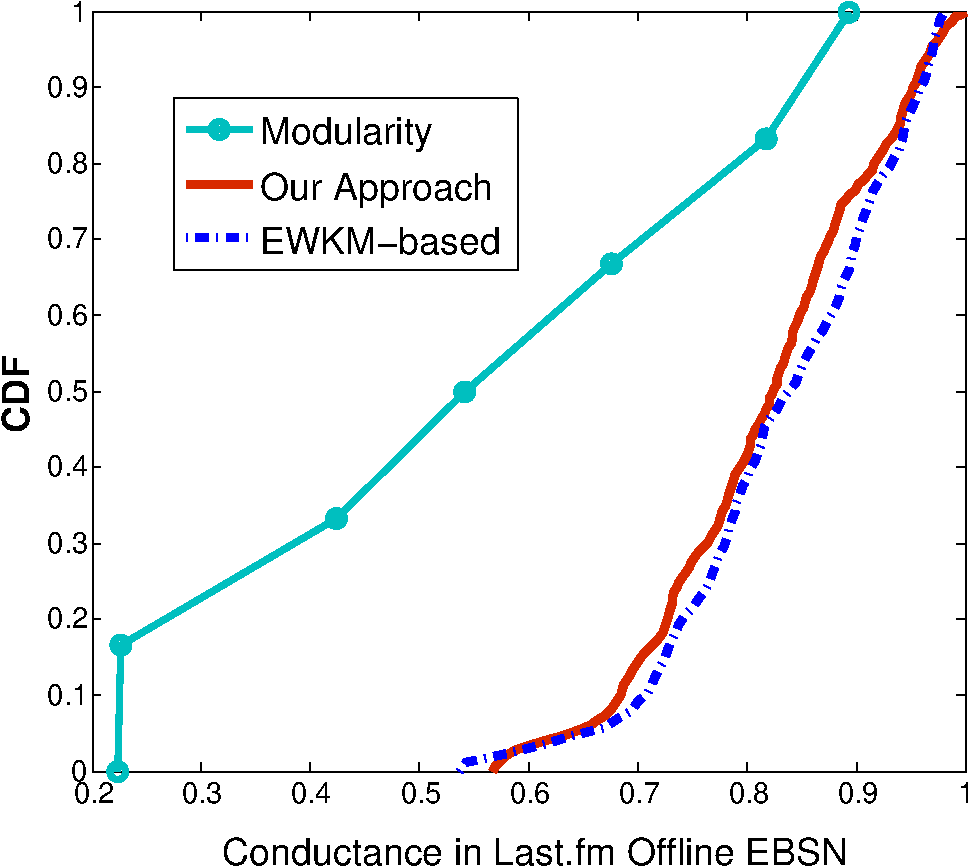
\includegraphics[height=60mm,width=67mm]{conductance-offline.pdf}}
\subfigure[]{\label{fig:conductance_b}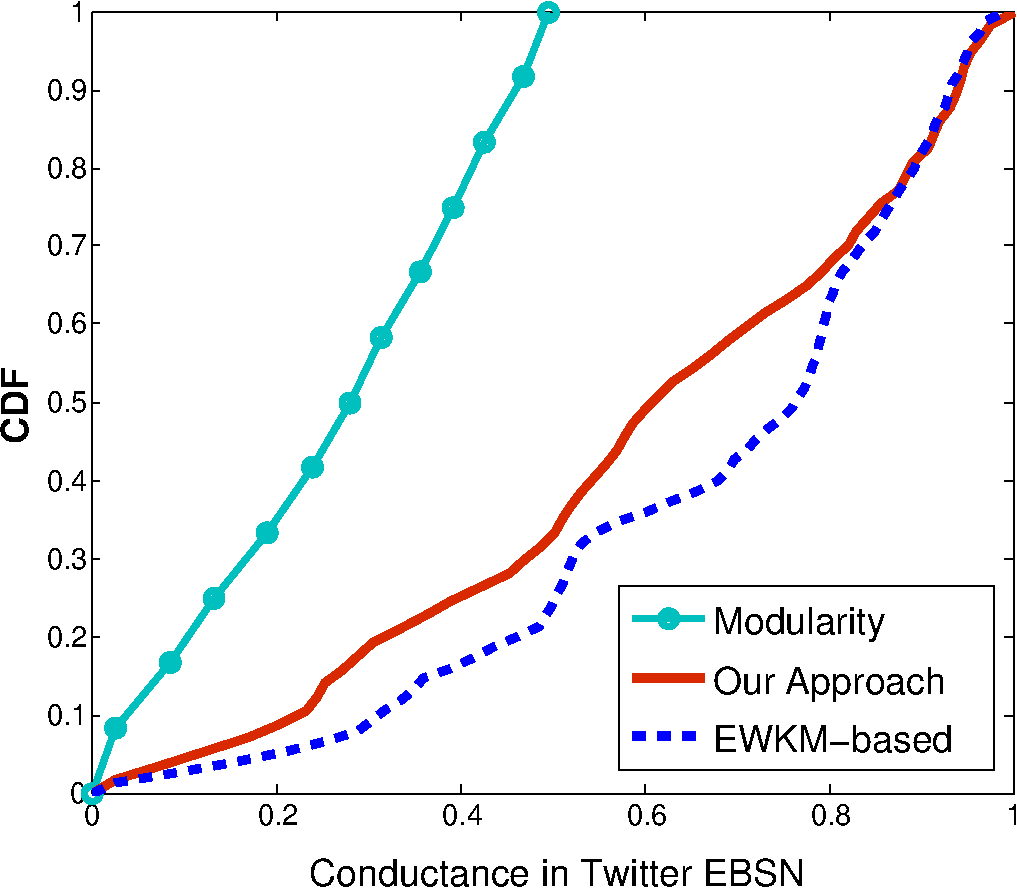
\includegraphics[height=60mm,width=63mm]{conductance-lanyrd.pdf}}
\caption{Conductance comparison in (a) Last.fm Offline EBSN and (b) Twitter EBSN}
\label{fig:conductance}
\end{figure}

It is difficult to construct a ground truth that represents the real communities within a network. Hence, we evaluate the proposed approach using the \emph{Conductance} metric~\cite{Leskovec:WWW08}. Conductance is a popular quality function assessing whether the detected communities are densely linked but weakly attached to the rest of the network. Note that this metric will evaluate our method from the link-based perspective. Lower conductance values mean better community structure. Figure~\ref{fig:conductance} shows the cumulative distribution (CDF) of the conductance respectively in Twitter EBSN and Last.fm Offline EBSN. Our approach produces slightly more communities with lower conductance values especially in Twitter EBSN. The reason behind is the strategy to determine users' memberships based on their global degrees. We believe that the better performance in Twitter EBSN is due to its clustering coefficient which is larger than that of Last.fm Offline EBSN.

\myparagraph{User Profiles Comparison} 
To evaluate our approach from the content-based perspective, one way is to compare the user profiles within one community. Hence, we retrieve the users' tags from each website and we only keep the frequent ones, thus creating a user profile. Cosine distance is then applied to compute the similarity between users' profiles. We consider that two users are similar when they have a Cosine distance above 0.3, a quite reasonable value considering the noisy tags. Figures~\ref{fig:comp-user} shows the CDF of the fraction of similar users within the same communities. It can be seen that our approach clustered more ``topically'' similar users than the EWKM-based method did. 


\begin{figure}[htb]
\centering
\subfigure[]{\label{fig:comp-user_a}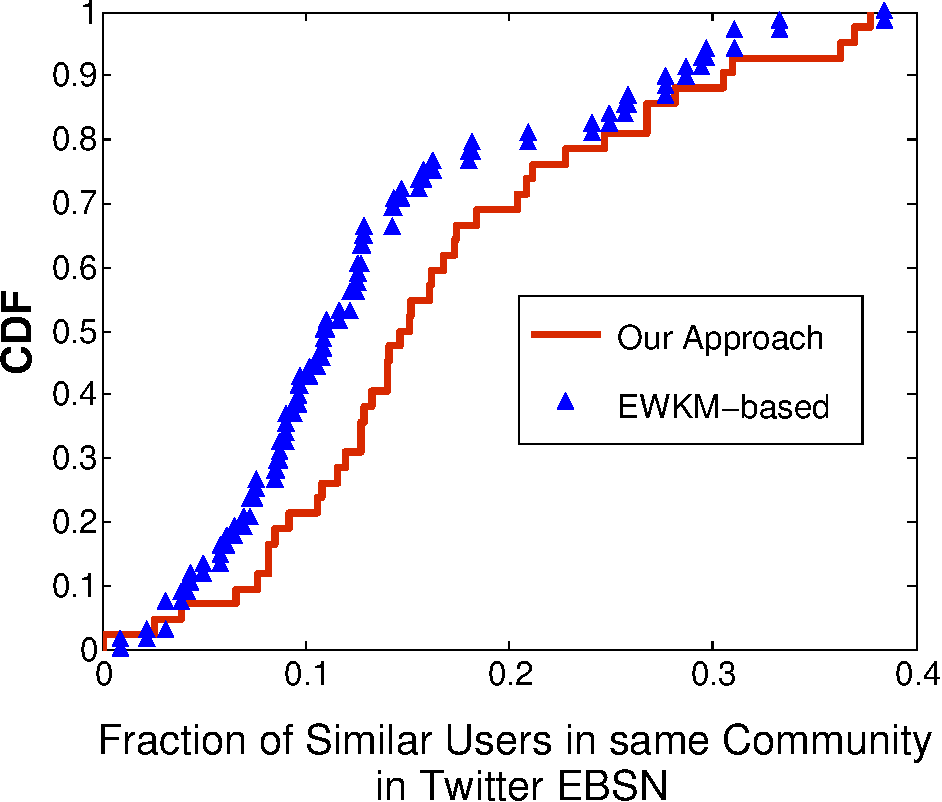
\includegraphics[height=63mm,width=68mm]{users-sim-lanyrd.pdf}}
\subfigure[]{\label{fig:comp-user_b}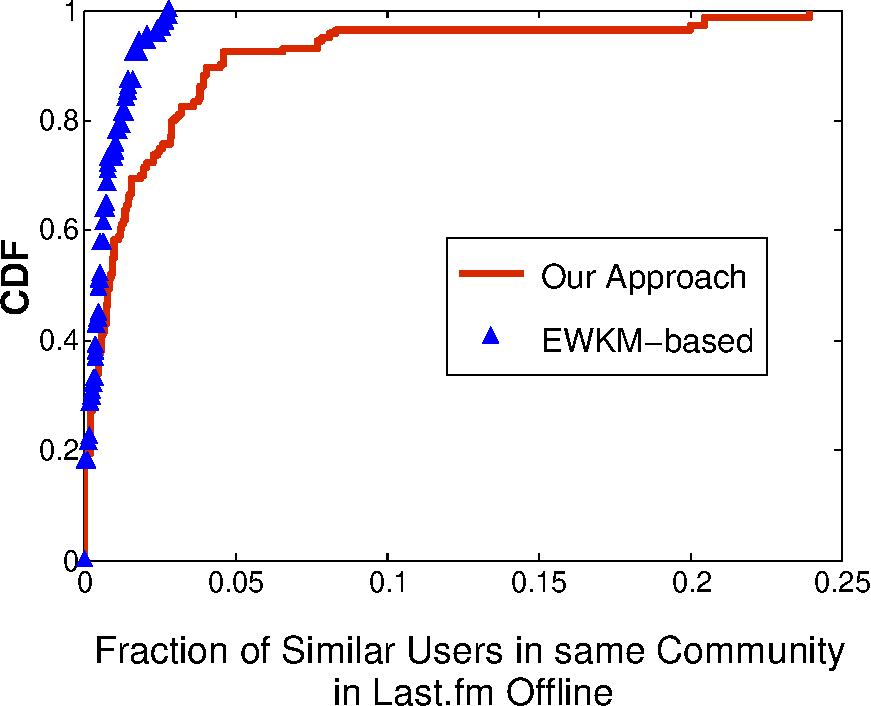
\includegraphics[height=64mm,width=68mm]{users-sim-offline.pdf}}
\caption{Comparison of user profiles in (a) Twitter EBSN and (b) Last.fm Offline EBSN}
\label{fig:comp-user}
\end{figure}

We also examine the fraction of ``friends''  within each community. The friendship information was extracted using the online social networks that exist in Last.fm and Twitter detected by our approach. Results are shown in Table~\ref{tab:friends}. We can see that a large fraction of friends were clustered in the same community by the Modularity method in Last.fm Offline EBSN compared with the other methods. This is also justified by the very high average size of communities detected which is equal to 474.5. Moreover, it is clearly shown that the conference attendees having similar topical interests are more likely to be friends than the case of concert attendees. 

\begin{table}[H]
\centering{
\begin{tabular}{ccc}
\hline
    \textbf{Method}    &   Twitter (Lanyrd) & Last.fm Offline \\
\hline
   Modularity-based  &  0.72 & 0.69\\
\hline
   EWKM-based  &   0.70 &0.23\\
\hline
   Our Approach  & 0.73   & 0.29\\
\hline
\end{tabular}
\caption{Average fraction of friends within communities}
\label{tab:friends}
}
\end{table}

\myparagraph{Communities Overlap} 

\begin{figure}[htb]
  \centering
  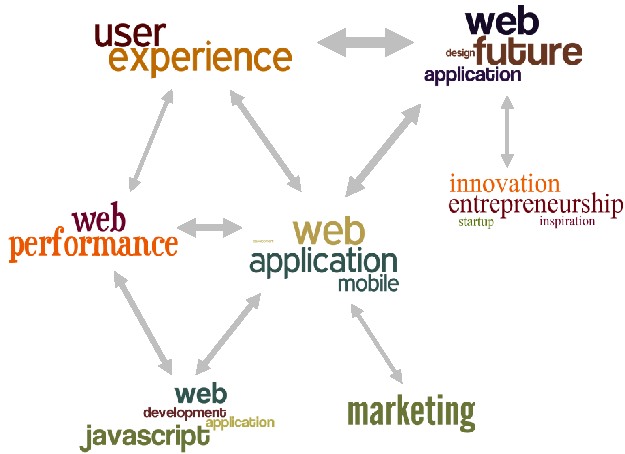
\includegraphics[scale=1]{tagCloudLanyrd.pdf}
  \caption{A sample of some overlapping communities in Twitter EBSN}
  \label{fig:tagcloud}
\end{figure}

Lastly, Figure~\ref{fig:tagcloud} shows a tag cloud representing a sample of the most overlapping communities in Twitter EBSN. The link thickness exhibits the overlapping degree. It can be drawn that the main topic of these communities is the Web domain which is the interest of many users who share different ``topical'' expertise. 

In Twitter EBSN, our approach detects 65 communities while the EWKM-based method produces 92 communities. Analyzing both community structures, it is found that our approach discovers fewer but more cohesive topical communities. We evaluate the cohesiveness using the popular Silhouette coefficient~\cite{Rousseeuw:1987}. For instance, we have detect only one community about the topic ``\emph{user experience}'' with a cohesion equal to 0.1. In contrast, 4 communities have been detected about this topic by the EWKM-based method including  2 singletons  (i.e. community having one user)  and having a cohesion equal to -0.3. This finding underlines the advantage of our approach to group together strongly linked users and to remove communities having weak connectivity.

\section{Conclusion}   \label{sec:conclusion}
Today's people use event and media websites to interact together either online by sharing comments and photos or offline by attending events. Thus, many social connections can be formed and strengthened during social events which can be considered as a basis to detect communities. In this chapter, we proposed a new approach to discover topical communities from event information. Taking into account both the content and the link information, we clustered events by maximizing a newly defined metric called \emph{Semantic Modularity}. Then, the user membership to each cluster was determined by a link-based function based on the user's degree. A comparison with existing studies shows the efficiency of our approach to detect communities optimizing both users connectivity and topical purity. Results highlighted how people interact differently in offline and online EBSN and how these interactions depend on the event category (e.g conference, concert, etc.). For future work, we plan to combine both the offline and the online worlds to solve community detection in a heterogeneous network. We wish to assess the impact of such combination on the purity and the connectivity of topical communities.
\chapter*{Conclusion of Part~\ref{pa:part2}}


This part has been devoted to put in use the Linked Data in event domain. Of a particular interest is the applications that handle better event presentation and discovery, as well as the personalization techniques.
\\
\\
Semantic Web applications have been developed to support end-users browsing and creating events. Overall, consuming Linked Data is advantageous to deliver enriched views of events, and to uncover interesting behavioral facts. Still, it was challenging to use conventional Web technologies on top of RDF data, a fact which reminds the trade-off between simplicity and expressivity.
\\
\\
Semantic Web technologies have been exploited to recommend events. Ontology-enabled feature extraction showed its ability to reduce the data sparsity, a problem from which suffers the traditional recommender systems. We highlighted that Linked Data is also beneficial to enrich data, thus improving the performance of our hybrid recommender system.
\\
\\
Finally, we proposed an approach to detect topical communities in event-based social network (EBSN) based on the content and link information. Linking events with media was particularly useful to construct EBSNs from media services. Evaluation shows how people interact differently from one service to another and depending on the event context.


\chapter{Conclusions and Future Perspectives}  \label{ch:conclusion}
\graphicspath{{conclusions/figures/}}

In this chapter, we summarize the major achievements of this thesis and we give an outlook on future perspectives.

\section{Scenario Flashback}

Going back to our scneario defined in Section~\ref{section:scenario}, we have defined two main personae. The first is a data analyst called \textbf{Dan} who works with the Ministry of Transport in France. He receives a memo from his management to create a report comparing the number of car accidents that occurred in France for this year, to its counterpart in the United Kingdom (UK). In addition, he is asked to highlight accidents related to illegal consumption of alcohol in both countries.

The second is a data portal administrator called \textbf{Paul}. He is affiliated with the British Open Data portal (\texttt{data.gov.uk}). His daily job includes acuqiring, preparing and publishing relevant datasets on the portal. He always strives to maintain a spam-free, high-quality portal.

\section{Achievements}

This thesis thouroughly describes the different steps aiming at realizing the vision of enabling self service data provisioning in the enterprise (see Figure~\ref{fig:architecutre_diagram_annotated}). The work presented is beneficial to both our personae introduced. The contributions made are:

\begin{adjustwidth}{-.4in}{-.4in}
	\begin{figure}[!ht]
	  \centering
	  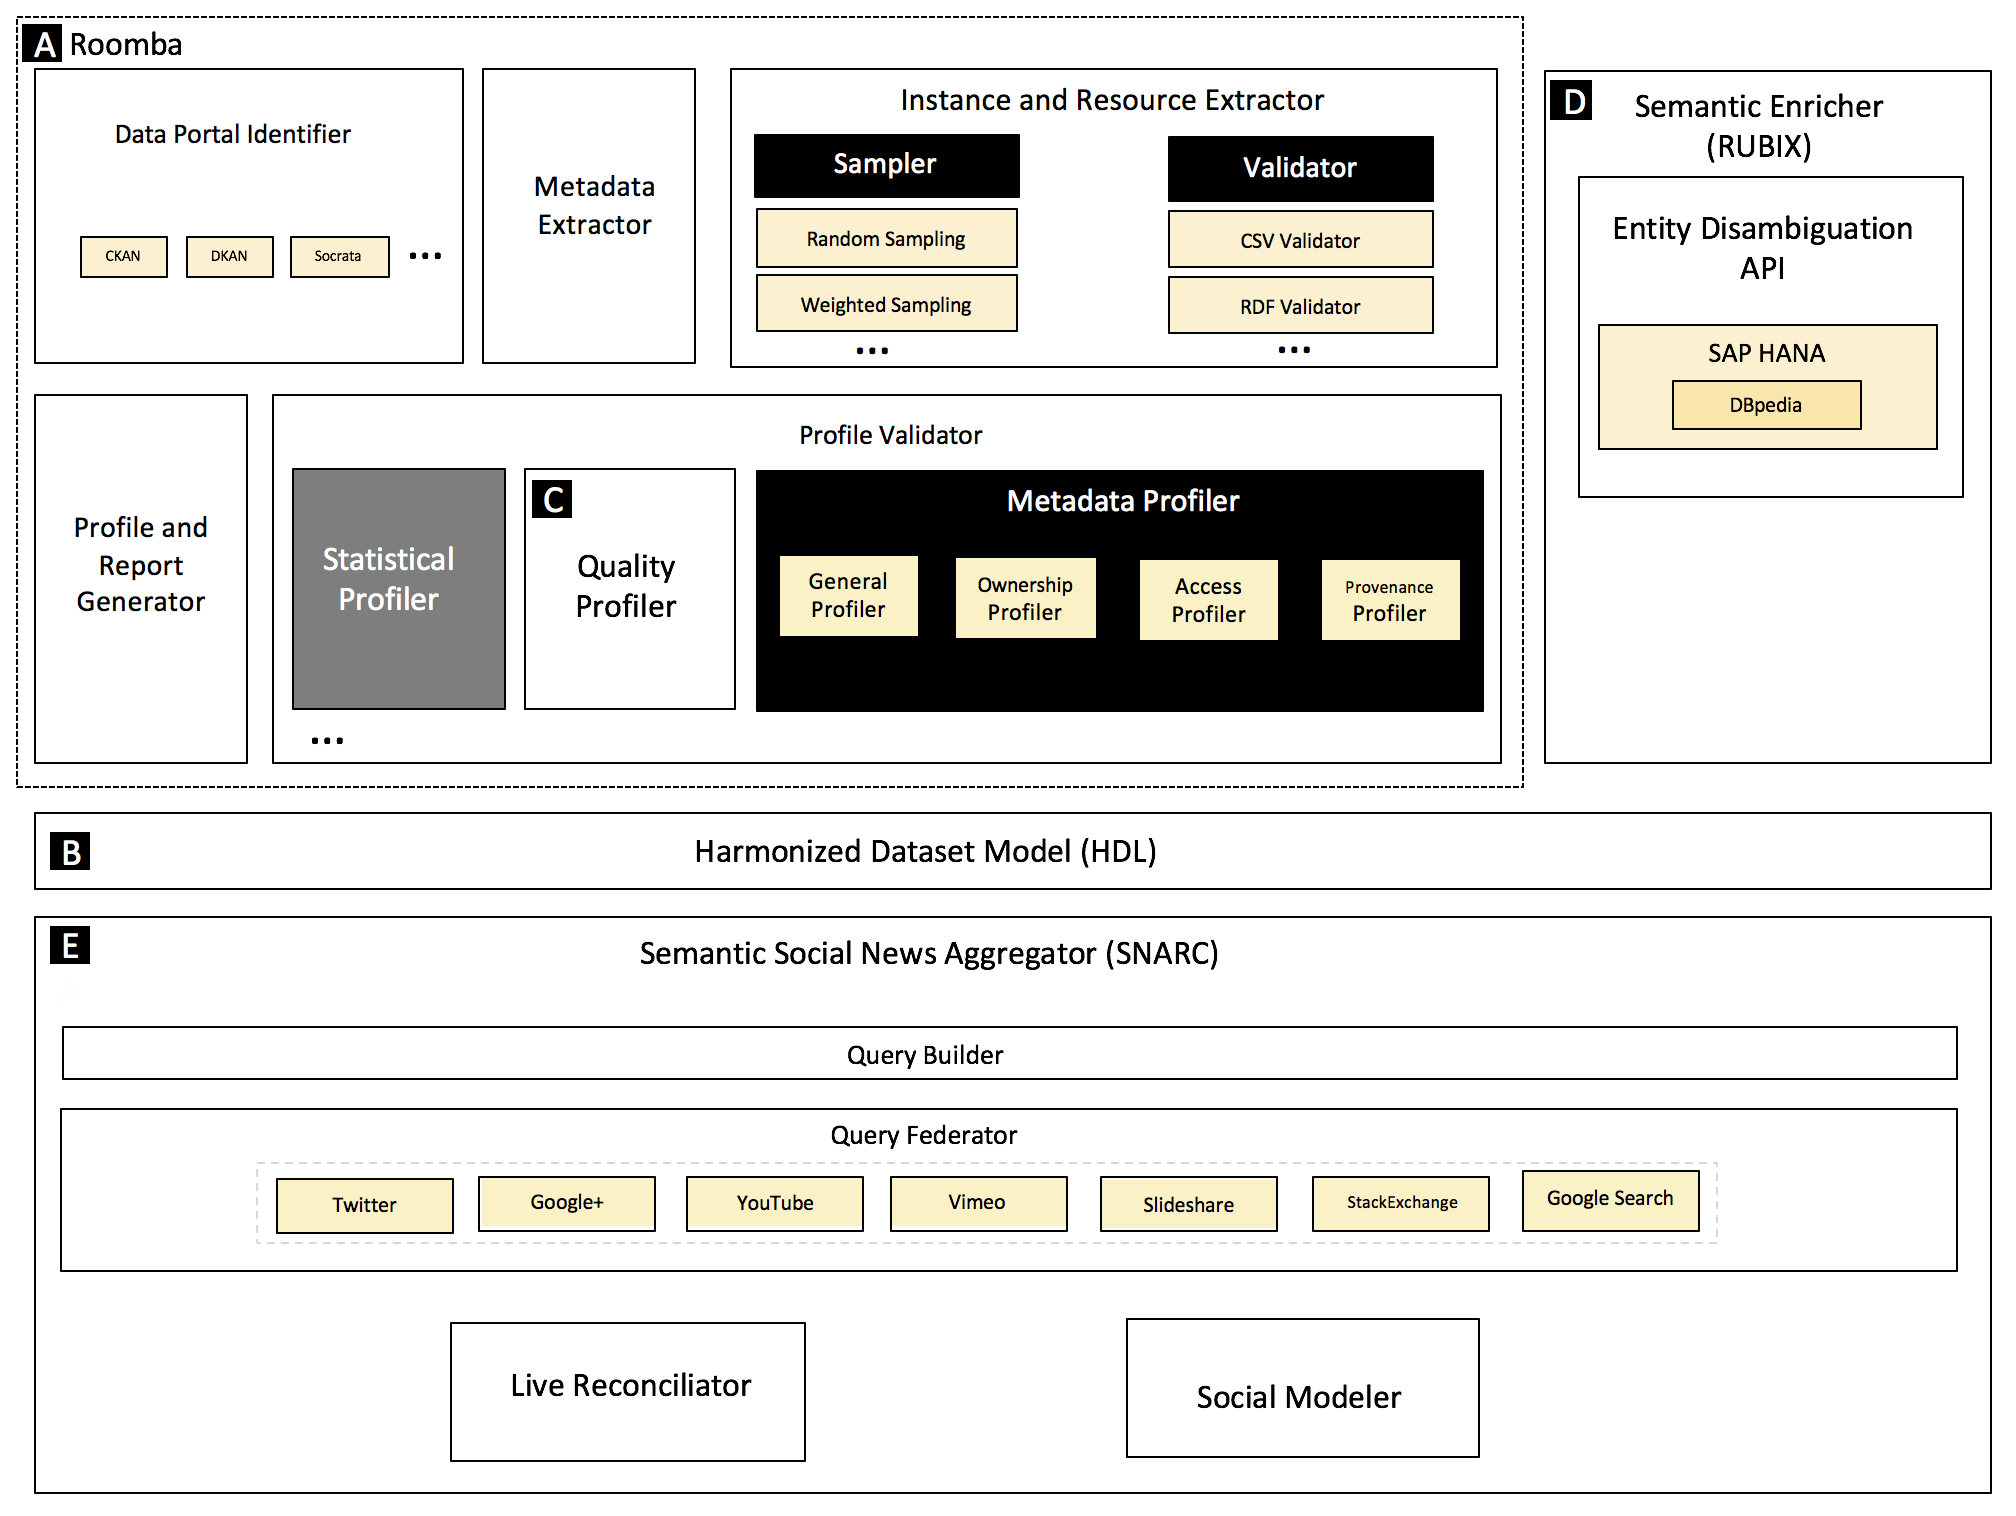
\includegraphics[scale=0.4]{architecutre_diagram_annotated.png}
	  \caption{Annoteted architecture diagram for enabling self-service data provisioning}
	  \label{fig:architecutre_diagram_annotated}
	\end{figure}
\end{adjustwidth}

\textbf{Contributions for Data Portals Administrators}
\vspace{1mm}
\\

Our data portal administrator \textbf{Paul} is always looking to expand his portals in terms of the number of datasets hosted, without compromising in their portal's data quality. In Chapter~\ref{chapter:hdl} (component \textbf{B} in Figure~\ref{fig:architecutre_diagram_annotated}), we surveyed the landscape of various models and vocabularies that described datasets on the web. We found a shortcoming when it comes to having a complete descriptive dataset model taking into account access, license and provenance information. As a result, we proposed a Harmonized Dataset Model (HDL) that \textbf{Paul} will use as a basis to extend and present the datasets he controls. \textbf{Paul} now also knows what are the major dataset models out there, and what kind of metadata data owners need to fully represent their dataset. The mappings proposed in Section~\ref{section:model_mappings} will allow him to easily integrate data from various data management systems into his own.

In Chapter~\ref{chapter:roomba} (component \textbf{A} in Figure~\ref{fig:architecutre_diagram_annotated}), we proposed Roomba, an automatic dataset profiles generation and validation tool that can be easily extended to perform various profiling tasks. Out of the box, \textbf{Paul} can use Roomba to automatically fix datasets metadata issues, and notify the datasets owners of the other issues to be manually fixed.

In Chapter~\ref{chapter:data-quality} (component \textbf{C} in Figure~\ref{fig:architecutre_diagram_annotated}), we proposed a comprehensive objective quality framework applied to the Linked Open Data. Moreover, after surveying the landscape of existing data quality tools, we identified several gaps and the need for a comprehensive evaluation and assessment framework and specifically for measuring quality on the dataset level. As a result, we presented an extension of Roomba that covers 82\% of the suggested datasets objective quality indicators. \textbf{Paul} will be able now to identify spam and low quality datasets. In addition to that, data available in his portal will now have rich semantic information attached to it. For example, temporal and spatial information extracted will be assigned into the corresponding fields in HDL. As an exemplary result, various datasets will be easily identifiable to cover various parts of the UK.\\

\textbf{Contributions for Data Analysts}
\vspace{1mm}\\

Our data analyst \textbf{Dan} believes that ``more data beats better algorithms'' and is always hunting for high quality data to produce accurate reports to the management team. By examining the rich datasets metadata presented in HDL he will be able to make fast decisions whether the dataset examined is suitable or not. He will also have vital information about the licensing and limitations for using this data internally. He will also have assurances on the dataset quality, which will help choose the best candidates out of ranked list.

\begin{wrapfigure}{r}{0.5\textwidth}
  \begin{center}
    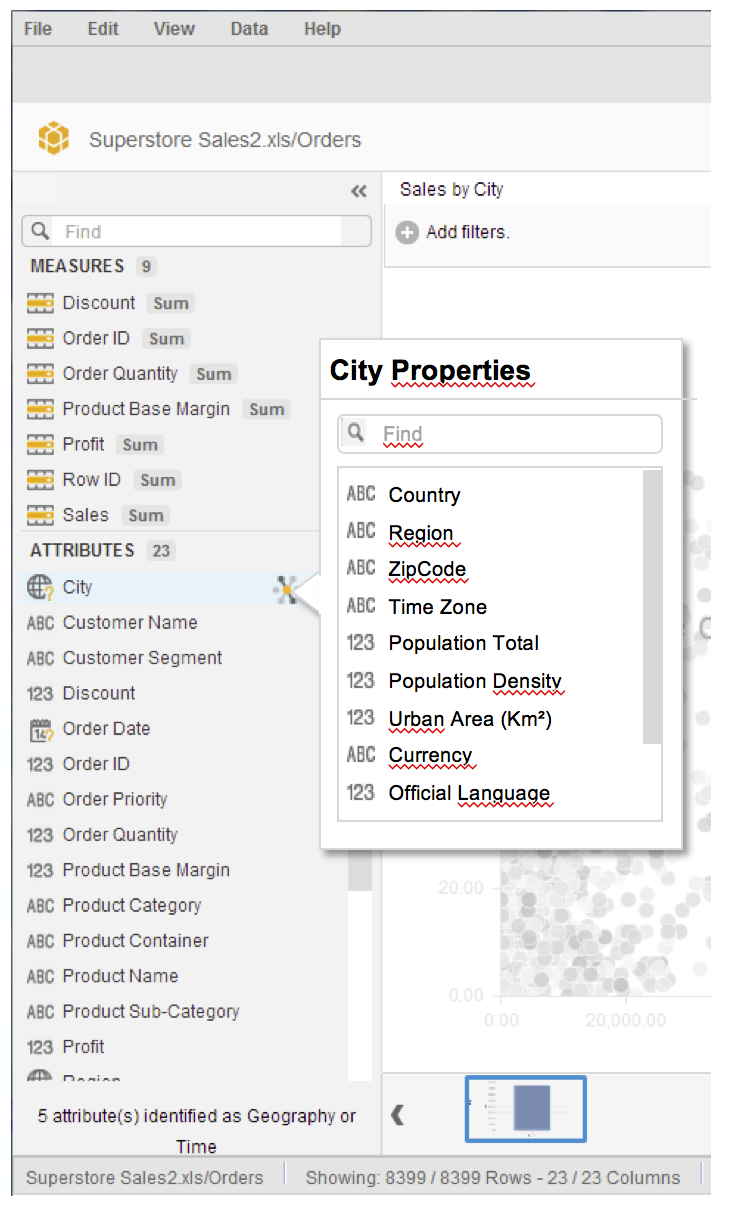
\includegraphics[width=0.48\textwidth]{lumira_sample.png}
  \end{center}
  \caption{UI Prototype of semantic data enrichment in SAP Lumira}
  \label{fig:lumira}
\end{wrapfigure}

\textbf{Dan} will be able to have direct access to rich and high-quality dataset descriptions generated by Roomba. Moreover, the topical profilers in Roomba will be able to identify occurrences of alcohol related terms like ``wine'' in various datasets. Query expansion methods can be used to relate alcohol to wine allowing him to find the datasets he wants.

In Chapter~\ref{chapter:rubix} component \textbf{D} in Figure~\ref{fig:architecutre_diagram_annotated}), we presented an entity disambiguation API built on top of SAP HANA. This API is used in RUBIX, a framework we proposed to enable mashup of potentially noisy enterprise and external data.
\textbf{Dan} now has access to various datasets that he found matching his query to the portal administered by \textbf{Paul}. He will be also able to use the schema matching services to find and merge those datasets in his reports.

Having imported those dataset into Lumira, he will be also able to use the internal knowledge base to apply various semantic enrichments on this data. Figure~\ref{fig:lumira} shows a possible integration of such service in SAP Lumira where \textbf{Dan} is presented with a ranked set of properties retrieved by the algorithm proposed in Section~\ref{Section:EKG}.

In Chapter~\ref{chapter:snarc} component \textbf{E} in Figure~\ref{fig:architecutre_diagram_annotated}), we proposed SNARC, a semantic social news aggregation service that allows the user to explore relevant news from internal or external sources. \textbf{Dan} is also a modern person, who is always trying to fresh information and believes in the wisdom of the crowd. Having SNARC services integrated with Lumira, he is also able to see a feed of relevant social media items that can be of interest to him. He actually follows a link in some tweet that he saw and was able to find relevant pieces of pointers that he would like to investigate further.

In summary, the contributions above pave the way to build a set of smart services to enable analysts easily find relevant pieces of information and administrators fight spam and be able to maintain high quality data portals. The work presented in this thesis goes beyond the fact that attaching metadata to datasets is vital, but propose a set of services that can automatically achieve that in seamless manner.

\section{Perspectives}

This thesis could be extended in the following directions:

\begin{itemize}

\item \textbf{Data Profile Representation}
\vspace{1mm}
\\
The proposed Harmonized Dataset Model (HDL) is currently available as a hierarchical JSON file. An enhancement would be to refine HDL and present it as a fully fledged OWL ontology. In addition, HDL can be extended to propose also a set of enumerations as values to ensure a unified fine-grained representation of a dataset. Moreover, while we presented the mappings between various models in a table structure, presenting those mappings in a machine readable format will allow various tools like Roomba to use it.

\item \textbf{Automatic Dataset Profiling}
\vspace{1mm}
\\
It has been noticed that the issues surrounding metadata quality affect directly dataset search as data portals rely on such information to power their search index. There are various extensions to our tool Roomba that can help in automatically building and enhancing dataset profiles. An example of these extension would be the integration of statistical and topical profilers allowing the generation of full comprehensive profiles. We would also like to extend Roomba to be able to run over other data portal types like DKAN or Socrata. This extension can be done by leveraging the data models mappings we proposed. In addition to all that, a possible enhancement will be ability to correct the rest of the metadata either automatically or through intuitive manually-driven interfaces.

\item \textbf{Objective Linked Data Quality}
\vspace{1mm}
\\
Ensuring data quality in Linked Open Data is a complex process as it consists of structured information supported by models, ontologies and vocabularies and contains queryable endpoints and links. In this thesis, we managed to narrow down the set of quality issues surrounding Linked Data to those who can be objectively measured and assessed by automatic tools. Our proposed tool covers 85\% of the quality indicators proposed. A possible extension would be to integrate tools assessing models quality in addition to syntactic checkers with Roomba. This will provide a complete coverage of the proposed quality indicators. Moreover, there are currently no weights assigned to the quality indicators. A valid contribution would be to suggest weights to those indicators which will result in a more objective quality calculation process.

\item \textbf{Enterprise Data Integration}
\vspace{1mm}
\\
A vital component to Data Integration in the enterprise is the existence of enterprise knowledge bases. Integrating additional linked open data sources of semantic types such as YAGO and evaluate our matching results against instance-based ontology alignment benchmarks such as OAEI\footnote{http://oaei.ontologymatching.org/2011/instance/index.html} or ISLab\footnote{http://islab.dico.unimi.it/iimb/} are possible future directions. Moreover, our work can be generalized to data classification. The same way the AMC helps identifying the best matches for two datasets, we plan to use it for identifying the best statistical classifiers for a sole dataset, based on normalized scores.
\end{itemize}

\appendix
\chapter*{List of Publications}

\section*{Journal}\label{sec:journals}

\begin{enumerate}
 \item \underline{\textbf{Ahmad Assaf}}, {R}apha{\"e}l {T}roncy and {A}line {S}enart: \textbf{Towards An Objective Assessment Framework for Linked Data Quality}. International Journal On Semantic Web and Information Systems, \emph{under review}, 2015.
\end{enumerate}

\section*{Conferences}\label{sec:conferences}

\begin{enumerate}
\item \underline{\textbf{Ahmad Assaf}}, {R}apha{\"e}l {T}roncy and {A}line {S}enart: \textbf{{A}utomatic Validation, Correction and Generation of Dataset Metadata - {E}nhancing Dataset Search and Spam Detection}. In 24th {I}nternational {W}orld {W}ide {W}eb {C}onference, Demo Track, May 2015, {F}lorence, {I}taly.
\item \underline{\textbf{Ahmad Assaf}}, {G}hislain {A}temezing, {R}apha{\"e}l {T}roncy and {E}lena {C}abrio: \textbf{{W}hat are the important properties of an entity? {C}omparing users and knowledge graph point of view}. In 11th {E}xtended {S}emantic {W}eb {C}onference (ESWC 2014), Demo Track, May 2014, {H}eraklion, {C}rete.
\item \underline{\textbf{Ahmad Assaf}}, {A}line {S}enart and {R}apha{\"e}l {T}roncy: \textbf{{SNARC} - An Approach for Aggregating and Recommending Contextualized Social Content}. In 10th {E}xtended {S}emantic {W}eb {C}onference (ESWC 2013), Sattelite Events, May 2013, {M}ontpellier, {F}rance. \textbf{1$^{st}$ Prize Winner of the AI Mashup Challenge}
\end{enumerate}

\section*{Workshops}\label{sec:workshops}

\begin{enumerate}
\item \underline{\textbf{Ahmad Assaf}}, {R}apha{\"e}l {T}roncy and {A}line {S}enart: \textbf{{W}hat's up {LOD} Cloud - Observing The State of Linked Open Data Cloud Metadata}. In 2nd Workshop on Linked Data Quality (LDQ), May 2015, {P}ortoroz, {S}lovenia. \textbf{Best paper award}
\item \underline{\textbf{Ahmad Assaf}}, {R}apha{\"e}l {T}roncy and {A}line {S}enart: \textbf{{HDL} - Towards A Harmonized Dataset Model for Open Data Portals}. In 2nd {I}nternational {W}orkshop on {D}ataset {PROFI}ling \& f{E}derated {S}earch for {L}inked {D}ata (PROFILES), May 2015, {P}ortoroz, {S}lovenia.
\item \underline{\textbf{Ahmad Assaf}}, {R}apha{\"e}l {T}roncy and {A}line {S}enart: \textbf{{A}n Extensible Framework to Validate and Build Dataset Profiles}. In 2nd {I}nternational {W}orkshop on {D}ataset {PROFI}ling \& f{E}derated {S}earch for {L}inked {D}ata (PROFILES), May 2015, {P}ortoroz, {S}lovenia. \textbf{Best paper award}
\item \underline{\textbf{Ahmad Assaf}}, {A}line {S}enart and {R}apha{\"e}l {T}roncy: \textbf{{D}ata Quality Principles in the Semantic Web}. International Workshop on Data Quality Management and Semantic Technologies, July 2012, {P}alermo, {I}taly.
\item \underline{\textbf{Ahmad Assaf}}, {E}ldad {L}ouw, {A}line {S}enart, {C}orentin {F}ollenfant {R}apha{\"e}l {T}roncy and {D}avid {T}rastour: \textbf{{RUBIX}: a Framework for Improving Data Integration with Linked Data}. In 1st International Workshop on Open Data (WOD), June 2012, {N}antes, {F}rance.
\end{enumerate}
\chapter{Optimization Techniques} \label{app:optimization}
In this appendix, we overview some technical aspects used in this thesis. More precisely, we describe two artificial intelligence techniques namely the Genetic Algorithms and the Particle Swarm Optimization widely used in optimization problems.

\section{Genetic Algorithms (GAs)}
Genetic Algorithms are stochastic methods inspired by the mechanism of natural evolution and genetic inheritance~\cite{Yeh:LRIR07}. GAs are are one of the most popular evolutionary algorithms widely used for solving optimization problems in many areas such as machine learning and image processing.  The idea behind is that the best solution can be found by combining the ``good'' parts of other solutions.

In GAs, a population is a set of \emph{chromosomes} (candidate solutions) and each chromosome denotes a set of \emph{genes}. The content of each gene is called \emph{allele}. A key component in GAs is the setting of a fitness criterion which accurately evaluates the quality of candidate solutions. First, a population of chromosomes are randomly generated and evaluated using the fitness function. The chromosomes having higher fitness values than others are stochastically selected, recombined and mutated to produce a new population for the next generation. To achieve this, GA has a set of key operators, namely \emph{selection}, \emph{crossover} and \emph{mutation}. The selection operator is used to select chromosomes called \emph{parents} to create the descendants of the next generation. The selection usually favored fitter patents, and there are approaches proposed in the literature. One example is the \emph{Stochastic Universal Sampling (SUS)} developed by Baker~\cite{Baker:1987}, which is used in this thesis. Consider a line where each chromosome occupies a segment proportional to the chromosome's fitness. \emph{SUS} uses $N$ equally spaced pointers placed over the line, where $N$ is the number of selections required.

Once parents for new population are chosen, genetic operators are applied such as crossover and mutation. Crossover refers to the recombination of parents to form a child. In particular, we used the scattered crossover which creates a random binary mask, then selecting the genes where the mask is 1 from one parent, and the rest from other parent. In order to force the algorithm exploring new areas in the search space, mutation is performed which alters at least one gene in a chromosome according to a predefined probability. Mutation rarely occurs in nature, which can justify the typical value 0.01 generally used as a mutation probability. Finally, the algorithm stops iterating when the optimal solution is produced or a maximal number of iterations is reached.

\section{Particle Swarm Optimization (PSO)}
It is a population-based stochastic optimization technique inspired by the social behavior of bird flocking or fish schooling~\cite{Kennedy:ICNN95}. PSO is similar to evolutionary algorithms and it was introduced in 1995 by Kennedy and Eberhat. Compared with GA, PSO is easy to implement with few parameters to adjust, and each individual  benefits from its history whereas no such mechanism exists in GA. PSO has been successfully applied to solving a wide range of optimization problems in different fields such as robotics, image, neural network, and information retrieval.

PSO simulates a group of birds searching for food in a bounded area, where the best position is the one containing the highest density of food. At the beginning, all the birds start searching for food randomly. Each bird knows two positions: its own position (i.e. history) found with the most of food and the best position from the whole swarm. The birds will be guided by these two positions in the search process until optimal convergence.

The PSO algorithm initializes a population of random solutions called \emph{swarms} or \emph{particles}, and searches for the optimal solution of a fitness function by updating generations. In each generation, each particle accelerates in the direction of its own personal best solution found so far, as well as in the direction of the global best position discovered so far by any of the particles in the swarm. This means that if a particle discovers a promising new solution, all the other particles will move closer to it, exploring the region more thoroughly in the search process. Each particle $i$ in the swarm has the following attributes: a current position $x_{i}$, a current velocity $v_{i}$, and a personal best position $p_{i}$ in the search space, and the global best position $p_{gbest}$ among all the $p_{i}$. In each iteration, the velocity and the position of each particle is updated as following:

\begin{gather*}
  v_{i}(t+1)= w . v_{i}(t) + c_{1} r_{1} (p_{i} - x_{i}(t)) + c_{2} r_{2} (p_{gbest} - x_{i}(t)) \\
  x_{i}(t+1)=x_{i}(t)+v_{i}(t+1) \\
\end{gather*}
where $c_{1}$ is the acceleration coefficient for each particle to move to its personal best position, $c_{2}$ is the acceleration coefficient to move to the global best position, $r_{1}$ and $r_{2}$ are random numbers uniformly distributed within [0,1], and $w$ is the inertia weight which controls the contribution of a particle's previous velocity to its current velocity. The velocity and acceleration are responsible for changing the position of the particle to explore the space of all possible solutions, instead of using existing solutions to reproduce. The personal and the global best positions are the optima of a predefined fitness function, respectively in each iteration and for all past iterations. In this thesis, to adjust some PSO parameters, we followed the setting recommended by Eberhart and Shi~\cite{Eberhart:CEC01}.
\chapter{String Similarity} \label{app:similarity}
There are different classes of string similarity functions. In this appendix, we focus on the main classes surveyed in the literature and we overview the most popular functions in each class. The similarity formulas described in this appendix compare two strings $s$ and $t$ which are associated with two token sets $S=s_1,s_2,...,s_n$ and $T=t_1,t_2,...,t_m$, respectively. For the computation, we used the Similarity Metric Library available online\footnote{\url{http://sourceforge.net/projects/simmetrics}}.

\section{Token-based Functions} 

The first family of the string similarity is the token-based functions which consider a string as a set of tokens. Intuitively, tokens also called ``bag of words'' are substrings generated by a tokenization function  (e.g. typically by a whitespace) applied on the original string. Making use of token-based functions is advantageous to overcome the word swaps. For example, the similarity between \emph{Mahatma Gandhi} and \emph{Gandhi Mahatma} will be maximal as both strings share the same tokens. However, the main drawback of such functions is to penalize approximate tokens having few spelling variations. That is, the comparison of \emph{brother} and \emph{brothers} will be zero.

One popular function is the Jaccard similarity~\cite{Jaccard:BVSN1901} which is the ratio of the intersection size and the union size of two token sets:

\begin{equation*}
 Jaccard(S,T)=\frac{|S \cap T|}{|S \cup T|}
\end{equation*}

Q-gram is another function which splits a string into small overlapping (i.e. common characters) units of size $q$. To obtain such units with the first and last characters of a string, we introduce a padding character (e.g. \Hash). For example, the 3-grams of \emph{Gandhi} is the set \textit{(\Hash \Hash G,\Hash Ga,Gan,and,ndh,dhi,hi\Hash ,i\Hash \Hash)}. Then, Jaccard function is typically used based on these tokens to compute the similarity score. 

The drawbacks of Jaccard is that it is very sensitive to spelling errors and it significantly penalizes  the unmatched tokens. In contrast, q-gram is less sensitive to spelling errors or to unmatched tokens. This comparison is illustrated in Table~\ref{tab:stringcomp}.

\begin{table}[H]
\footnotesize{
 \begin{center}
  \begin{tabular}{cccc}
  \hline
  String s & String t & Jaccard  & 3-gram \\
  \hline
  Johnny Depp & Johny Dep & 0 & 0.75\\
  \hline 
  sir Johnny Depp & Mr Johnny Depp & 0.5 & 0.78 \\
  \hline 
  \end{tabular}
  \caption{Comparison between Jaccard and 3-gram}
  \label{tab:stringcomp}
 \end{center}}
\end{table}

Cosine distance is another typical token-based function used in Information Retrieval for high dimensional data. Given two n-dimensional vectors X and Y containing the weights of tokens, the Cosine distance is defined as the cosine angle between these two vectors:

\begin{equation*}
 Cosine(X,Y)=\frac{|X \cdot Y|}{\norm{X} \cdot \norm{Y}} = \frac {\sum_{i=1}^{n} x_i \cdot y_i} {\sqrt{\sum_{i=1}^{n} x^{2}_i} \cdot \sqrt{\sum_{i=1}^{n} y^{2}_i}}
\end{equation*}
In particular, the TF-IDF Cosine is commonly used where each token has a weight according to Term Frequency-Inverse Document Frequency scheme. This scheme is composed of two measures: term frequency ($tf$) and  inverse document frequency ($idf$). The intuition behind the term frequency is that the more often a token occurs in a given string, the higher is its contribution to the similarity. In contrast, the inverse document frequency assigns higher weights to rare tokens in all the corpus (all the strings or documents). For each token $s_i$ from the string $s$, the IF-IDF score is:

\begin{equation*}
 tf\textrm{-}idf_{i,s}= tf_{i,s} \cdot log \left(\frac{D}{D(t_i)}\right)
\end{equation*}
where $tf_{i,s}$ is the term frequency of $s_i$ in the string $s$, $D$ is the number of the strings in the corpus, $D(i)$ is the number of strings that contain the token $s_i$ in the corpus. The computation of Cosine distance can be enhanced by hashing functions due to the high sparsity of most vectors. The advantage to use Cosine distance is to take into account the relative importance of different tokens in long strings and text documents.

\section{Character-based Functions}

The second family of string similarity is the character-based function also called edit-based similarity. Unlike the token-based functions, a string is considered as an ordered sequence of characters instead of a set of tokens. They allow different ``edit operations'' necessary to transform one string to another such as deletion, insertion, substitution, and transposition of characters. The use of these functions is mainly performed on short strings to overcome spelling errors. However, the performance of these functions drastically decreases when changing the order of the tokens.

One popular function is the Levenshtein distance~\cite{Levenshtein:SPD66} that allows three edit operations which are the deletion, insertion, and substitution. The score is equal to the minimum number of operations required to transform $s$ to $t$. For example, to transform \textit{Maria} to \textit{Mario}, we need the replace $a$ by $o$, which gives a similarity score equal to 1. The normalized score is equal to 0.8. One drawback of Levenshtein is that it is not adapted for some variations such as abbreviations (e.g. \emph{Gandhi Mahatma} and \emph{Gandhi M}) or extra prefix (e.g. \emph{Sir Gandhi} and \emph{Gandhi}).

A similar metric is the Jaro distance~\cite{Jaro:JASA89} which allows character transpositions and based on the number and the order of common characters. Two characters are considered to be common if they are equal and if the distance between their positions $i$ and $j$ within the two strings does not exceed $H$, where $H=0.5 \times min(|s|,|t|)$. Given a set of common characters $\sigma$, a transposition occurs if the $i^{th}$ common character of $s$ is different from the $i^{th}$ common character of $t$. Let $\theta$ is half the number of transpositions, Jaro is computed as:

\begin{equation*}
		Jaro (s,t) =  \frac{1}{3} \times  \left(  \frac{|\sigma|}{|s|} +\frac{|\sigma|}{|t|} + \frac{|\sigma|-\theta}{|\sigma|} \right) 
\end{equation*}
Jaro distance performs well when there is few spelling variations. However, as common characters have to occur in a specific distance, variations such as a long prefix in one string (e.g. $s=\textit{Doctor John Smith}$ and $t=\textit{John Smith}$) yields a low similarity of 0.46. A variant of Jaro distance, called Jaro-Winkler similarity~\cite{Winkler:1999} uses the length of the longest common prefix to emphasize matches in the first $p$ characters of the two strings. For example the Jaro similarity between \textit{John S} and \textit{John Smith} is 0.86, while the Jaro-Winkler score is 0.94.

\section{Hybrid Functions} 
To overcome the limitations of character and token based functions, the metrics in the third family combines both of them, also referred as hybrid functions.

Extended Jaccard similarity is a hybrid function proposed to also include not only the equals tokens, but also the similar ones in the the original Jaccard function~\cite{Weis:SIGMOD05,Ananthakrishna:VLDB02}. Consider \textit{TokenSim} be a string similarity metric that compares two tokens $s_i$ and $t_j$, and $\theta$ is the related threshold, the set of shared similar tokens between $s$ and $t$ is defined as:

\begin{equation*}
	Shared (s,t)=\lbrace (s_i,t_j) | s_i \in S \wedge t_j \in T: TokenSim(s_i,t_j)\geqslant \theta \rbrace
\end{equation*}
The set of unique or unmatched tokens in $s$ is defined as:

\begin{equation*}
	Unique(s)=\lbrace s_i | s_i \in S \wedge t_j \in T \wedge (s_i,t_j) \notin Shared \rbrace
\end{equation*}
Similarly, we define the set $Unique(t)$ for the string $t$. This has been extended by a function that gives weights $w$ to matched and unmatched tokens, which are combined using an aggregation function $Ag$. The hybrid Jaccard is defined as:
\vspace{-2mm}
\begin{gather*}
	matched=Ag_{(s_i,t_j) \in Shared (s,t)} {\ } w(s_i,t_j) \\[1mm]
	unmatched=Ag_{(s_i) \in Unique(s)}  {\ } w(s_i)  + Ag_{(t_j) \in Unique(t)} {\ }  w(t_j)  \\[1mm]
	HybridJaccard(s,t)= \frac{matched}{matched+unmatched}
\end{gather*}
Note that different weights could be given for the tokens in $Shared (s,t)$, $Unique(s)$, and $Unique(t$). For instance, let s= \textit{Mindy Smith} and t=\textit{Minndy Smith Festival}, the hybrid Jaccard generates the following sets: 
\begin{gather*}
Shared(s,t)= \lbrace (Mindy,Minndy),(Smith,Smith) \rbrace \\[1mm]
 Unique(s)= \varnothing  \\[1mm]
 Unique(t)=  \lbrace Festival \rbrace
\end{gather*}
Assuming that the weights of matched tokens is their normalized Levenshtein similarity, and the weights of unmatched tokens is equal to 1. If the aggregate function $Ag$ simply sums the weights, the hybrid Jaccard is:  

\begin{equation*}
	HybridJaccard(s,t)=\frac{0.83+1}{0.83+1+0+1}=0.64
\end{equation*}
Note that the score remains low due to the influence of unmatched tokens. The Token-Wise metric proposed in Section~\ref{sec:metric-similarity} follows the same rationale, but gives more importance to similar tokens. Moreover, the weight of unmatched tokens takes into account the fact that the two token sets have different sizes. In this example, the weight for unmatched tokens is equal to $\frac{2}{3}=0.66$. We obtain higher score than hybrid Jaccard when using Token-wise:

\begin{equation*}
	Token\textrm{-}Wise(s,t)=\frac{2 \times (0.83+1)}{2 \times (0.83+1)+ 0.66 \times (0+1)}=0.84
\end{equation*}
Another hybrid function is the Monge-Elkan similarity~\cite{Monge:KDD96} that matches every token $s_i$ from $s$ with the token $t_j$ in $t$ having the maximum similarity using \textit{TokenSim} metric. Monge-Elkan is defined as:

\begin {equation*}
MongeElkan(s,t) = \frac{1}{|S|} {\ } \sum_{i=1}^{|S|}  \max_{j=1}^{|T|} {\ } TokenSim(s_i,t_j)
\end {equation*}
Given the strings $s=$ \textit{Mindy Smith} and $t=$ \textit{Minndy Smith Festival}, and using Levenshtein as \textit{TokenSim}, the Monge-Elkan score is:

\begin{equation*}
	MongeElkan(s,t)=\frac{0.83+1}{2}=0.91
\end{equation*}
Monge-Elkan is sensitive to the size of the first string. For instance, if $t$ is the first string which is of length 3, the Monge-Elkan score decreases to 0.61.
\\
\\
The last hybrid function is called SoftTFIDF~\cite{Cohen:IIWeb03} which extends the Cosine similarity, following the same rationale as hybrid Jaccard. Let $CLOSE(\theta, S, T)$ be the set of words $s_i \in S$ such that there is $t_j \in T$ where $TokenSim(s_i,t_j) > \theta$, and $maxsim(s_i,t_j)=max(\lbrace TokenSim(s_i,t_j) | t_j\in T \rbrace)$. The SoftTFIDF is defined as:

\begin {equation*}
SoftTFIDF(s,t) = \sum_{s_i \in CLOSE(\theta, S, T)} \left( \frac{tf\textrm{-}idf_{s_i}}{\norm{X}} \cdot \frac{tf\textrm{-}idf_{t_j}}{\norm{Y}} \times maxsim(s_i,t_j) \right) 
\end {equation*}
where $X$ and $Y$ are the vector representations of $s$ and $t$ containing the $tf\textrm{-}idf$ scores of related tokens, respectively. Given the strings $s=$ \textit{Mindy Smith} and $t=$\textit{Minndy Smith Festival} and unit weights for all the tokens (no corpus considered), the SoftTFIDF gives:

\begin{equation*}
	SoftTFIDF(s,t)=\frac{1}{\sqrt{2}} \times \frac{1}{\sqrt{3}} \times 0.83 + \frac{1}{\sqrt{2}} \times \frac{1}{\sqrt{3}} \times 1 =0.75
\end{equation*}

\chapter{Recommender Systems} \label{app:recommendation}
\graphicspath{{appendix/}}
Broadly speaking, the recommender systems are based on two popular strategies: the content-based filtering and the collaborative filtering. In the following, we overview the basic concepts about those techniques. 

\section{Content-based Recommendation}               \label{sec:content-recommendation}
The content-based systems exploit the attributes characterizing an item or a user. They analyze the content information collected explicitly or implicitly to construct a user or an item profile. The matching between both profiles can be quantified using a variety of similarity distances such as Cosine similarity, Pearson correlation and Latent Semantic Analysis~\cite{Deerwester:ASIS90}. This kind of matching is also applied to discover people sharing similar interests. It is closely related to detecting documents of similar content in information retrieval field. A known successful realization of content-based filtering is the Music Genome Project which is used for the Internet radio service Pandora.com. In this project, a trained music system ranks each song  based on hundreds of distinct musical characteristics. These attributes or genes capture not only a song's musical identity but also many significant qualities which are relevant to understanding listeners' musical preferences~\cite{Koren:ICS2009}. Another interesting study proposed by Chen at al.~\cite{Chen:ICHF2009} compare different recommender algorithms in the IBM's enterprise social networking service called ``Beehive''. The authors underline that the pure content matching is the most effective to recommend unknown friends and in general diverse items. However, the  content-based recommendation has the drawback to not take into account the information in preference similarity across individuals.

\section{Collaborative Filtering Recommendation}               \label{sec:collaborative-filtering}
The second strategy of recommender system is based on collaborative filtering(CF), a technique that does not need an explicit content profiling and purely rely on past user behavior~\cite{Herlocker:CSCW00}. It has been widely applied in many well-known services such as Amazon, Faceboook, LinkedIn, MySpace and Last.fm. The basis is to analyze the relationships between users and inter-dependencies among items to identify new user-item associations. In other words, the system makes automatic predictions (filtering) about the user interests based on the preferences of like-minded and similar users (collaborating). The intuition behind is that if a person A has the same preference as a person B on an item, A is more likely to have B's preference on another item, as illustrated in Figure~\ref{fig:user-cf}.

\begin{figure}[H]
  \centering
  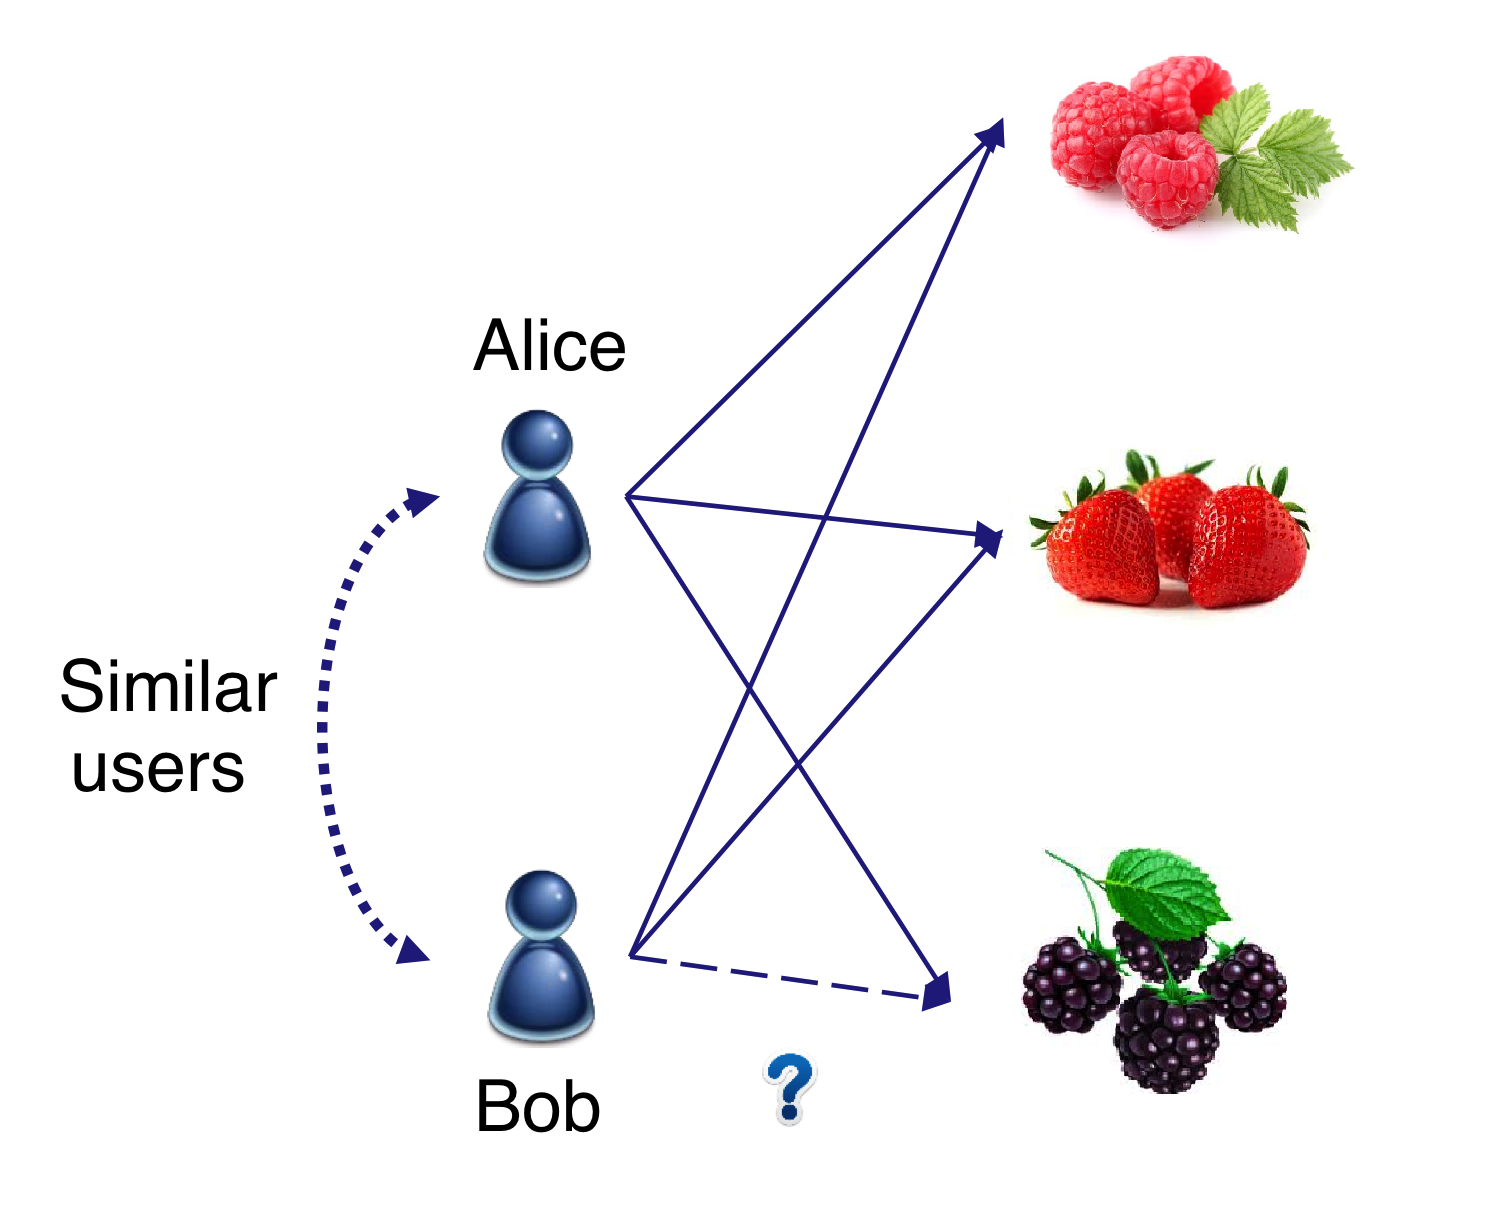
\includegraphics[scale=0.15]{user-cf.png}
  \caption{user-based collaborative filtering: Alice has a crush on berry fruits, Bob also likes two of them. The recommender system understands that Alice and Bob have similar tastes, and Bob is recommended the Blackberry}
  \label{fig:user-cf}
\end{figure}

There exists two primary categories of collaborative filtering which are memory-based and model-based approaches. The memory-based systems compute the similarity between users or, alternatively, between items based on users preferences data, thus detecting the neighbors of a given user or item. Indeed, the unknown rating value of the active user \emph{u} for an item \emph{m} is an aggregation of the ratings of users similar to \emph{u} for the same item \emph{m}, or an aggregation of the ratings of the user \emph{u} to similar items of \emph{m}. The model-based systems, on the other hand, use data mining and machine learning algorithms to estimate or learn a model from observed ratings to make predictions. A typical example is the latent factor model that discovers unobserved factors from ratings patterns. The underlying assumption is that there is a set of common hidden factors which explain a set of observations in co-occurrence data. More precisely, the similarity between users and items is simultaneously induced by some hidden lower-dimensional structure in the data. Recently, several matrix factorization methods~\cite{Koren:ICS2009} have been proposed as a successful realization of latent factor model. The users and items are simultaneously represented as unknown feature vectors within a user-item matrix. These feature vectors are learnt using low-rank approximations, so that they approximate the known preference ratings with respect to some loss measure. Despite the important success of collaborative filtering, it still suffers from three serious limitations: the sparsity problem where there are few ratings about items, the cold-start problem where items have no ratings, and the scalability where a large amount of users and items have to be analyzed.



\bibliographystyle{plain}
\bibliography{thesis}

\chapter*{}
\chaptermark{}
%\section*{}
%\sectionmark{}
\vspace{-15ex}
%\appendix
\end{document}
